% !TEX root = ./article.tex
\appendix
\section{Derivative Equation Generated Data Example}
\begin{figure}[H]
  \centering
  \begin{subfigure}{\linewidth}
    \begin{adjustbox}{width=\linewidth}
      \begingroup%
\makeatletter%
\begin{pgfpicture}%
\pgfpathrectangle{\pgfpointorigin}{\pgfqpoint{8.000000in}{2.000000in}}%
\pgfusepath{use as bounding box, clip}%
\begin{pgfscope}%
\pgfsetbuttcap%
\pgfsetmiterjoin%
\pgfsetlinewidth{0.000000pt}%
\definecolor{currentstroke}{rgb}{0.000000,0.000000,0.000000}%
\pgfsetstrokecolor{currentstroke}%
\pgfsetstrokeopacity{0.000000}%
\pgfsetdash{}{0pt}%
\pgfpathmoveto{\pgfqpoint{0.000000in}{0.000000in}}%
\pgfpathlineto{\pgfqpoint{8.000000in}{0.000000in}}%
\pgfpathlineto{\pgfqpoint{8.000000in}{2.000000in}}%
\pgfpathlineto{\pgfqpoint{0.000000in}{2.000000in}}%
\pgfpathlineto{\pgfqpoint{0.000000in}{0.000000in}}%
\pgfpathclose%
\pgfusepath{}%
\end{pgfscope}%
\begin{pgfscope}%
\pgfsetbuttcap%
\pgfsetmiterjoin%
\pgfsetlinewidth{0.000000pt}%
\definecolor{currentstroke}{rgb}{0.000000,0.000000,0.000000}%
\pgfsetstrokecolor{currentstroke}%
\pgfsetstrokeopacity{0.000000}%
\pgfsetdash{}{0pt}%
\pgfpathmoveto{\pgfqpoint{0.593772in}{0.517039in}}%
\pgfpathlineto{\pgfqpoint{7.958330in}{0.517039in}}%
\pgfpathlineto{\pgfqpoint{7.958330in}{1.958330in}}%
\pgfpathlineto{\pgfqpoint{0.593772in}{1.958330in}}%
\pgfpathlineto{\pgfqpoint{0.593772in}{0.517039in}}%
\pgfpathclose%
\pgfusepath{}%
\end{pgfscope}%
\begin{pgfscope}%
\pgfsetbuttcap%
\pgfsetroundjoin%
\definecolor{currentfill}{rgb}{0.000000,0.000000,0.000000}%
\pgfsetfillcolor{currentfill}%
\pgfsetlinewidth{0.803000pt}%
\definecolor{currentstroke}{rgb}{0.000000,0.000000,0.000000}%
\pgfsetstrokecolor{currentstroke}%
\pgfsetdash{}{0pt}%
\pgfsys@defobject{currentmarker}{\pgfqpoint{0.000000in}{-0.048611in}}{\pgfqpoint{0.000000in}{0.000000in}}{%
\pgfpathmoveto{\pgfqpoint{0.000000in}{0.000000in}}%
\pgfpathlineto{\pgfqpoint{0.000000in}{-0.048611in}}%
\pgfusepath{stroke,fill}%
}%
\begin{pgfscope}%
\pgfsys@transformshift{0.928524in}{0.517039in}%
\pgfsys@useobject{currentmarker}{}%
\end{pgfscope}%
\end{pgfscope}%
\begin{pgfscope}%
\definecolor{textcolor}{rgb}{0.000000,0.000000,0.000000}%
\pgfsetstrokecolor{textcolor}%
\pgfsetfillcolor{textcolor}%
\pgftext[x=0.928524in,y=0.419816in,,top]{\color{textcolor}{\rmfamily\fontsize{12.000000}{14.400000}\selectfont\catcode`\^=\active\def^{\ifmmode\sp\else\^{}\fi}\catcode`\%=\active\def%{\%}0.00}}%
\end{pgfscope}%
\begin{pgfscope}%
\pgfsetbuttcap%
\pgfsetroundjoin%
\definecolor{currentfill}{rgb}{0.000000,0.000000,0.000000}%
\pgfsetfillcolor{currentfill}%
\pgfsetlinewidth{0.803000pt}%
\definecolor{currentstroke}{rgb}{0.000000,0.000000,0.000000}%
\pgfsetstrokecolor{currentstroke}%
\pgfsetdash{}{0pt}%
\pgfsys@defobject{currentmarker}{\pgfqpoint{0.000000in}{-0.048611in}}{\pgfqpoint{0.000000in}{0.000000in}}{%
\pgfpathmoveto{\pgfqpoint{0.000000in}{0.000000in}}%
\pgfpathlineto{\pgfqpoint{0.000000in}{-0.048611in}}%
\pgfusepath{stroke,fill}%
}%
\begin{pgfscope}%
\pgfsys@transformshift{1.765406in}{0.517039in}%
\pgfsys@useobject{currentmarker}{}%
\end{pgfscope}%
\end{pgfscope}%
\begin{pgfscope}%
\definecolor{textcolor}{rgb}{0.000000,0.000000,0.000000}%
\pgfsetstrokecolor{textcolor}%
\pgfsetfillcolor{textcolor}%
\pgftext[x=1.765406in,y=0.419816in,,top]{\color{textcolor}{\rmfamily\fontsize{12.000000}{14.400000}\selectfont\catcode`\^=\active\def^{\ifmmode\sp\else\^{}\fi}\catcode`\%=\active\def%{\%}0.25}}%
\end{pgfscope}%
\begin{pgfscope}%
\pgfsetbuttcap%
\pgfsetroundjoin%
\definecolor{currentfill}{rgb}{0.000000,0.000000,0.000000}%
\pgfsetfillcolor{currentfill}%
\pgfsetlinewidth{0.803000pt}%
\definecolor{currentstroke}{rgb}{0.000000,0.000000,0.000000}%
\pgfsetstrokecolor{currentstroke}%
\pgfsetdash{}{0pt}%
\pgfsys@defobject{currentmarker}{\pgfqpoint{0.000000in}{-0.048611in}}{\pgfqpoint{0.000000in}{0.000000in}}{%
\pgfpathmoveto{\pgfqpoint{0.000000in}{0.000000in}}%
\pgfpathlineto{\pgfqpoint{0.000000in}{-0.048611in}}%
\pgfusepath{stroke,fill}%
}%
\begin{pgfscope}%
\pgfsys@transformshift{2.602287in}{0.517039in}%
\pgfsys@useobject{currentmarker}{}%
\end{pgfscope}%
\end{pgfscope}%
\begin{pgfscope}%
\definecolor{textcolor}{rgb}{0.000000,0.000000,0.000000}%
\pgfsetstrokecolor{textcolor}%
\pgfsetfillcolor{textcolor}%
\pgftext[x=2.602287in,y=0.419816in,,top]{\color{textcolor}{\rmfamily\fontsize{12.000000}{14.400000}\selectfont\catcode`\^=\active\def^{\ifmmode\sp\else\^{}\fi}\catcode`\%=\active\def%{\%}0.50}}%
\end{pgfscope}%
\begin{pgfscope}%
\pgfsetbuttcap%
\pgfsetroundjoin%
\definecolor{currentfill}{rgb}{0.000000,0.000000,0.000000}%
\pgfsetfillcolor{currentfill}%
\pgfsetlinewidth{0.803000pt}%
\definecolor{currentstroke}{rgb}{0.000000,0.000000,0.000000}%
\pgfsetstrokecolor{currentstroke}%
\pgfsetdash{}{0pt}%
\pgfsys@defobject{currentmarker}{\pgfqpoint{0.000000in}{-0.048611in}}{\pgfqpoint{0.000000in}{0.000000in}}{%
\pgfpathmoveto{\pgfqpoint{0.000000in}{0.000000in}}%
\pgfpathlineto{\pgfqpoint{0.000000in}{-0.048611in}}%
\pgfusepath{stroke,fill}%
}%
\begin{pgfscope}%
\pgfsys@transformshift{3.439169in}{0.517039in}%
\pgfsys@useobject{currentmarker}{}%
\end{pgfscope}%
\end{pgfscope}%
\begin{pgfscope}%
\definecolor{textcolor}{rgb}{0.000000,0.000000,0.000000}%
\pgfsetstrokecolor{textcolor}%
\pgfsetfillcolor{textcolor}%
\pgftext[x=3.439169in,y=0.419816in,,top]{\color{textcolor}{\rmfamily\fontsize{12.000000}{14.400000}\selectfont\catcode`\^=\active\def^{\ifmmode\sp\else\^{}\fi}\catcode`\%=\active\def%{\%}0.75}}%
\end{pgfscope}%
\begin{pgfscope}%
\pgfsetbuttcap%
\pgfsetroundjoin%
\definecolor{currentfill}{rgb}{0.000000,0.000000,0.000000}%
\pgfsetfillcolor{currentfill}%
\pgfsetlinewidth{0.803000pt}%
\definecolor{currentstroke}{rgb}{0.000000,0.000000,0.000000}%
\pgfsetstrokecolor{currentstroke}%
\pgfsetdash{}{0pt}%
\pgfsys@defobject{currentmarker}{\pgfqpoint{0.000000in}{-0.048611in}}{\pgfqpoint{0.000000in}{0.000000in}}{%
\pgfpathmoveto{\pgfqpoint{0.000000in}{0.000000in}}%
\pgfpathlineto{\pgfqpoint{0.000000in}{-0.048611in}}%
\pgfusepath{stroke,fill}%
}%
\begin{pgfscope}%
\pgfsys@transformshift{4.276051in}{0.517039in}%
\pgfsys@useobject{currentmarker}{}%
\end{pgfscope}%
\end{pgfscope}%
\begin{pgfscope}%
\definecolor{textcolor}{rgb}{0.000000,0.000000,0.000000}%
\pgfsetstrokecolor{textcolor}%
\pgfsetfillcolor{textcolor}%
\pgftext[x=4.276051in,y=0.419816in,,top]{\color{textcolor}{\rmfamily\fontsize{12.000000}{14.400000}\selectfont\catcode`\^=\active\def^{\ifmmode\sp\else\^{}\fi}\catcode`\%=\active\def%{\%}1.00}}%
\end{pgfscope}%
\begin{pgfscope}%
\pgfsetbuttcap%
\pgfsetroundjoin%
\definecolor{currentfill}{rgb}{0.000000,0.000000,0.000000}%
\pgfsetfillcolor{currentfill}%
\pgfsetlinewidth{0.803000pt}%
\definecolor{currentstroke}{rgb}{0.000000,0.000000,0.000000}%
\pgfsetstrokecolor{currentstroke}%
\pgfsetdash{}{0pt}%
\pgfsys@defobject{currentmarker}{\pgfqpoint{0.000000in}{-0.048611in}}{\pgfqpoint{0.000000in}{0.000000in}}{%
\pgfpathmoveto{\pgfqpoint{0.000000in}{0.000000in}}%
\pgfpathlineto{\pgfqpoint{0.000000in}{-0.048611in}}%
\pgfusepath{stroke,fill}%
}%
\begin{pgfscope}%
\pgfsys@transformshift{5.112932in}{0.517039in}%
\pgfsys@useobject{currentmarker}{}%
\end{pgfscope}%
\end{pgfscope}%
\begin{pgfscope}%
\definecolor{textcolor}{rgb}{0.000000,0.000000,0.000000}%
\pgfsetstrokecolor{textcolor}%
\pgfsetfillcolor{textcolor}%
\pgftext[x=5.112932in,y=0.419816in,,top]{\color{textcolor}{\rmfamily\fontsize{12.000000}{14.400000}\selectfont\catcode`\^=\active\def^{\ifmmode\sp\else\^{}\fi}\catcode`\%=\active\def%{\%}1.25}}%
\end{pgfscope}%
\begin{pgfscope}%
\pgfsetbuttcap%
\pgfsetroundjoin%
\definecolor{currentfill}{rgb}{0.000000,0.000000,0.000000}%
\pgfsetfillcolor{currentfill}%
\pgfsetlinewidth{0.803000pt}%
\definecolor{currentstroke}{rgb}{0.000000,0.000000,0.000000}%
\pgfsetstrokecolor{currentstroke}%
\pgfsetdash{}{0pt}%
\pgfsys@defobject{currentmarker}{\pgfqpoint{0.000000in}{-0.048611in}}{\pgfqpoint{0.000000in}{0.000000in}}{%
\pgfpathmoveto{\pgfqpoint{0.000000in}{0.000000in}}%
\pgfpathlineto{\pgfqpoint{0.000000in}{-0.048611in}}%
\pgfusepath{stroke,fill}%
}%
\begin{pgfscope}%
\pgfsys@transformshift{5.949814in}{0.517039in}%
\pgfsys@useobject{currentmarker}{}%
\end{pgfscope}%
\end{pgfscope}%
\begin{pgfscope}%
\definecolor{textcolor}{rgb}{0.000000,0.000000,0.000000}%
\pgfsetstrokecolor{textcolor}%
\pgfsetfillcolor{textcolor}%
\pgftext[x=5.949814in,y=0.419816in,,top]{\color{textcolor}{\rmfamily\fontsize{12.000000}{14.400000}\selectfont\catcode`\^=\active\def^{\ifmmode\sp\else\^{}\fi}\catcode`\%=\active\def%{\%}1.50}}%
\end{pgfscope}%
\begin{pgfscope}%
\pgfsetbuttcap%
\pgfsetroundjoin%
\definecolor{currentfill}{rgb}{0.000000,0.000000,0.000000}%
\pgfsetfillcolor{currentfill}%
\pgfsetlinewidth{0.803000pt}%
\definecolor{currentstroke}{rgb}{0.000000,0.000000,0.000000}%
\pgfsetstrokecolor{currentstroke}%
\pgfsetdash{}{0pt}%
\pgfsys@defobject{currentmarker}{\pgfqpoint{0.000000in}{-0.048611in}}{\pgfqpoint{0.000000in}{0.000000in}}{%
\pgfpathmoveto{\pgfqpoint{0.000000in}{0.000000in}}%
\pgfpathlineto{\pgfqpoint{0.000000in}{-0.048611in}}%
\pgfusepath{stroke,fill}%
}%
\begin{pgfscope}%
\pgfsys@transformshift{6.786696in}{0.517039in}%
\pgfsys@useobject{currentmarker}{}%
\end{pgfscope}%
\end{pgfscope}%
\begin{pgfscope}%
\definecolor{textcolor}{rgb}{0.000000,0.000000,0.000000}%
\pgfsetstrokecolor{textcolor}%
\pgfsetfillcolor{textcolor}%
\pgftext[x=6.786696in,y=0.419816in,,top]{\color{textcolor}{\rmfamily\fontsize{12.000000}{14.400000}\selectfont\catcode`\^=\active\def^{\ifmmode\sp\else\^{}\fi}\catcode`\%=\active\def%{\%}1.75}}%
\end{pgfscope}%
\begin{pgfscope}%
\pgfsetbuttcap%
\pgfsetroundjoin%
\definecolor{currentfill}{rgb}{0.000000,0.000000,0.000000}%
\pgfsetfillcolor{currentfill}%
\pgfsetlinewidth{0.803000pt}%
\definecolor{currentstroke}{rgb}{0.000000,0.000000,0.000000}%
\pgfsetstrokecolor{currentstroke}%
\pgfsetdash{}{0pt}%
\pgfsys@defobject{currentmarker}{\pgfqpoint{0.000000in}{-0.048611in}}{\pgfqpoint{0.000000in}{0.000000in}}{%
\pgfpathmoveto{\pgfqpoint{0.000000in}{0.000000in}}%
\pgfpathlineto{\pgfqpoint{0.000000in}{-0.048611in}}%
\pgfusepath{stroke,fill}%
}%
\begin{pgfscope}%
\pgfsys@transformshift{7.623577in}{0.517039in}%
\pgfsys@useobject{currentmarker}{}%
\end{pgfscope}%
\end{pgfscope}%
\begin{pgfscope}%
\definecolor{textcolor}{rgb}{0.000000,0.000000,0.000000}%
\pgfsetstrokecolor{textcolor}%
\pgfsetfillcolor{textcolor}%
\pgftext[x=7.623577in,y=0.419816in,,top]{\color{textcolor}{\rmfamily\fontsize{12.000000}{14.400000}\selectfont\catcode`\^=\active\def^{\ifmmode\sp\else\^{}\fi}\catcode`\%=\active\def%{\%}2.00}}%
\end{pgfscope}%
\begin{pgfscope}%
\definecolor{textcolor}{rgb}{0.000000,0.000000,0.000000}%
\pgfsetstrokecolor{textcolor}%
\pgfsetfillcolor{textcolor}%
\pgftext[x=4.276051in,y=0.202965in,,top]{\color{textcolor}{\rmfamily\fontsize{12.000000}{14.400000}\selectfont\catcode`\^=\active\def^{\ifmmode\sp\else\^{}\fi}\catcode`\%=\active\def%{\%}Time (hours)}}%
\end{pgfscope}%
\begin{pgfscope}%
\pgfsetbuttcap%
\pgfsetroundjoin%
\definecolor{currentfill}{rgb}{0.000000,0.000000,0.000000}%
\pgfsetfillcolor{currentfill}%
\pgfsetlinewidth{0.803000pt}%
\definecolor{currentstroke}{rgb}{0.000000,0.000000,0.000000}%
\pgfsetstrokecolor{currentstroke}%
\pgfsetdash{}{0pt}%
\pgfsys@defobject{currentmarker}{\pgfqpoint{-0.048611in}{0.000000in}}{\pgfqpoint{-0.000000in}{0.000000in}}{%
\pgfpathmoveto{\pgfqpoint{-0.000000in}{0.000000in}}%
\pgfpathlineto{\pgfqpoint{-0.048611in}{0.000000in}}%
\pgfusepath{stroke,fill}%
}%
\begin{pgfscope}%
\pgfsys@transformshift{0.593772in}{0.714824in}%
\pgfsys@useobject{currentmarker}{}%
\end{pgfscope}%
\end{pgfscope}%
\begin{pgfscope}%
\definecolor{textcolor}{rgb}{0.000000,0.000000,0.000000}%
\pgfsetstrokecolor{textcolor}%
\pgfsetfillcolor{textcolor}%
\pgftext[x=0.260881in, y=0.651510in, left, base]{\color{textcolor}{\rmfamily\fontsize{12.000000}{14.400000}\selectfont\catcode`\^=\active\def^{\ifmmode\sp\else\^{}\fi}\catcode`\%=\active\def%{\%}\ensuremath{-}2}}%
\end{pgfscope}%
\begin{pgfscope}%
\pgfsetbuttcap%
\pgfsetroundjoin%
\definecolor{currentfill}{rgb}{0.000000,0.000000,0.000000}%
\pgfsetfillcolor{currentfill}%
\pgfsetlinewidth{0.803000pt}%
\definecolor{currentstroke}{rgb}{0.000000,0.000000,0.000000}%
\pgfsetstrokecolor{currentstroke}%
\pgfsetdash{}{0pt}%
\pgfsys@defobject{currentmarker}{\pgfqpoint{-0.048611in}{0.000000in}}{\pgfqpoint{-0.000000in}{0.000000in}}{%
\pgfpathmoveto{\pgfqpoint{-0.000000in}{0.000000in}}%
\pgfpathlineto{\pgfqpoint{-0.048611in}{0.000000in}}%
\pgfusepath{stroke,fill}%
}%
\begin{pgfscope}%
\pgfsys@transformshift{0.593772in}{1.174158in}%
\pgfsys@useobject{currentmarker}{}%
\end{pgfscope}%
\end{pgfscope}%
\begin{pgfscope}%
\definecolor{textcolor}{rgb}{0.000000,0.000000,0.000000}%
\pgfsetstrokecolor{textcolor}%
\pgfsetfillcolor{textcolor}%
\pgftext[x=0.390511in, y=1.110844in, left, base]{\color{textcolor}{\rmfamily\fontsize{12.000000}{14.400000}\selectfont\catcode`\^=\active\def^{\ifmmode\sp\else\^{}\fi}\catcode`\%=\active\def%{\%}0}}%
\end{pgfscope}%
\begin{pgfscope}%
\pgfsetbuttcap%
\pgfsetroundjoin%
\definecolor{currentfill}{rgb}{0.000000,0.000000,0.000000}%
\pgfsetfillcolor{currentfill}%
\pgfsetlinewidth{0.803000pt}%
\definecolor{currentstroke}{rgb}{0.000000,0.000000,0.000000}%
\pgfsetstrokecolor{currentstroke}%
\pgfsetdash{}{0pt}%
\pgfsys@defobject{currentmarker}{\pgfqpoint{-0.048611in}{0.000000in}}{\pgfqpoint{-0.000000in}{0.000000in}}{%
\pgfpathmoveto{\pgfqpoint{-0.000000in}{0.000000in}}%
\pgfpathlineto{\pgfqpoint{-0.048611in}{0.000000in}}%
\pgfusepath{stroke,fill}%
}%
\begin{pgfscope}%
\pgfsys@transformshift{0.593772in}{1.633492in}%
\pgfsys@useobject{currentmarker}{}%
\end{pgfscope}%
\end{pgfscope}%
\begin{pgfscope}%
\definecolor{textcolor}{rgb}{0.000000,0.000000,0.000000}%
\pgfsetstrokecolor{textcolor}%
\pgfsetfillcolor{textcolor}%
\pgftext[x=0.390511in, y=1.570178in, left, base]{\color{textcolor}{\rmfamily\fontsize{12.000000}{14.400000}\selectfont\catcode`\^=\active\def^{\ifmmode\sp\else\^{}\fi}\catcode`\%=\active\def%{\%}2}}%
\end{pgfscope}%
\begin{pgfscope}%
\definecolor{textcolor}{rgb}{0.000000,0.000000,0.000000}%
\pgfsetstrokecolor{textcolor}%
\pgfsetfillcolor{textcolor}%
\pgftext[x=0.205325in,y=1.237684in,,bottom,rotate=90.000000]{\color{textcolor}{\rmfamily\fontsize{12.000000}{14.400000}\selectfont\catcode`\^=\active\def^{\ifmmode\sp\else\^{}\fi}\catcode`\%=\active\def%{\%}Velocity}}%
\end{pgfscope}%
\begin{pgfscope}%
\pgfpathrectangle{\pgfqpoint{0.593772in}{0.517039in}}{\pgfqpoint{7.364558in}{1.441291in}}%
\pgfusepath{clip}%
\pgfsetrectcap%
\pgfsetroundjoin%
\pgfsetlinewidth{1.505625pt}%
\definecolor{currentstroke}{rgb}{0.121569,0.466667,0.705882}%
\pgfsetstrokecolor{currentstroke}%
\pgfsetdash{}{0pt}%
\pgfpathmoveto{\pgfqpoint{0.928524in}{0.843191in}}%
\pgfpathlineto{\pgfqpoint{0.941941in}{0.865997in}}%
\pgfpathlineto{\pgfqpoint{0.955358in}{0.906286in}}%
\pgfpathlineto{\pgfqpoint{0.968775in}{0.959976in}}%
\pgfpathlineto{\pgfqpoint{1.009026in}{1.147828in}}%
\pgfpathlineto{\pgfqpoint{1.022443in}{1.200354in}}%
\pgfpathlineto{\pgfqpoint{1.035860in}{1.239395in}}%
\pgfpathlineto{\pgfqpoint{1.049277in}{1.261427in}}%
\pgfpathlineto{\pgfqpoint{1.062694in}{1.264405in}}%
\pgfpathlineto{\pgfqpoint{1.076111in}{1.247946in}}%
\pgfpathlineto{\pgfqpoint{1.089527in}{1.213370in}}%
\pgfpathlineto{\pgfqpoint{1.102944in}{1.163613in}}%
\pgfpathlineto{\pgfqpoint{1.116361in}{1.103010in}}%
\pgfpathlineto{\pgfqpoint{1.143195in}{0.971508in}}%
\pgfpathlineto{\pgfqpoint{1.156612in}{0.912884in}}%
\pgfpathlineto{\pgfqpoint{1.170029in}{0.867009in}}%
\pgfpathlineto{\pgfqpoint{1.183446in}{0.839030in}}%
\pgfpathlineto{\pgfqpoint{1.196863in}{0.832911in}}%
\pgfpathlineto{\pgfqpoint{1.210280in}{0.851116in}}%
\pgfpathlineto{\pgfqpoint{1.223697in}{0.894394in}}%
\pgfpathlineto{\pgfqpoint{1.237114in}{0.961703in}}%
\pgfpathlineto{\pgfqpoint{1.250531in}{1.050260in}}%
\pgfpathlineto{\pgfqpoint{1.263948in}{1.155723in}}%
\pgfpathlineto{\pgfqpoint{1.317615in}{1.624147in}}%
\pgfpathlineto{\pgfqpoint{1.331032in}{1.719454in}}%
\pgfpathlineto{\pgfqpoint{1.344449in}{1.794130in}}%
\pgfpathlineto{\pgfqpoint{1.357866in}{1.844122in}}%
\pgfpathlineto{\pgfqpoint{1.371283in}{1.866952in}}%
\pgfpathlineto{\pgfqpoint{1.384700in}{1.861870in}}%
\pgfpathlineto{\pgfqpoint{1.398117in}{1.829878in}}%
\pgfpathlineto{\pgfqpoint{1.411534in}{1.773634in}}%
\pgfpathlineto{\pgfqpoint{1.424951in}{1.697244in}}%
\pgfpathlineto{\pgfqpoint{1.438368in}{1.605959in}}%
\pgfpathlineto{\pgfqpoint{1.478619in}{1.304250in}}%
\pgfpathlineto{\pgfqpoint{1.492036in}{1.214953in}}%
\pgfpathlineto{\pgfqpoint{1.505453in}{1.140181in}}%
\pgfpathlineto{\pgfqpoint{1.518870in}{1.083720in}}%
\pgfpathlineto{\pgfqpoint{1.532286in}{1.047995in}}%
\pgfpathlineto{\pgfqpoint{1.545703in}{1.033964in}}%
\pgfpathlineto{\pgfqpoint{1.559120in}{1.041113in}}%
\pgfpathlineto{\pgfqpoint{1.572537in}{1.067552in}}%
\pgfpathlineto{\pgfqpoint{1.585954in}{1.110205in}}%
\pgfpathlineto{\pgfqpoint{1.599371in}{1.165065in}}%
\pgfpathlineto{\pgfqpoint{1.653039in}{1.412093in}}%
\pgfpathlineto{\pgfqpoint{1.666456in}{1.458232in}}%
\pgfpathlineto{\pgfqpoint{1.679873in}{1.491241in}}%
\pgfpathlineto{\pgfqpoint{1.693290in}{1.509362in}}%
\pgfpathlineto{\pgfqpoint{1.706707in}{1.511991in}}%
\pgfpathlineto{\pgfqpoint{1.720124in}{1.499674in}}%
\pgfpathlineto{\pgfqpoint{1.733541in}{1.474038in}}%
\pgfpathlineto{\pgfqpoint{1.746958in}{1.437637in}}%
\pgfpathlineto{\pgfqpoint{1.773791in}{1.346204in}}%
\pgfpathlineto{\pgfqpoint{1.787208in}{1.298977in}}%
\pgfpathlineto{\pgfqpoint{1.800625in}{1.256066in}}%
\pgfpathlineto{\pgfqpoint{1.814042in}{1.221157in}}%
\pgfpathlineto{\pgfqpoint{1.827459in}{1.197414in}}%
\pgfpathlineto{\pgfqpoint{1.840876in}{1.187278in}}%
\pgfpathlineto{\pgfqpoint{1.854293in}{1.192327in}}%
\pgfpathlineto{\pgfqpoint{1.867710in}{1.213182in}}%
\pgfpathlineto{\pgfqpoint{1.881127in}{1.249477in}}%
\pgfpathlineto{\pgfqpoint{1.894544in}{1.299881in}}%
\pgfpathlineto{\pgfqpoint{1.907961in}{1.362174in}}%
\pgfpathlineto{\pgfqpoint{1.934795in}{1.509914in}}%
\pgfpathlineto{\pgfqpoint{1.961629in}{1.662843in}}%
\pgfpathlineto{\pgfqpoint{1.975046in}{1.730907in}}%
\pgfpathlineto{\pgfqpoint{1.988463in}{1.788072in}}%
\pgfpathlineto{\pgfqpoint{2.001879in}{1.830870in}}%
\pgfpathlineto{\pgfqpoint{2.015296in}{1.856453in}}%
\pgfpathlineto{\pgfqpoint{2.028713in}{1.862741in}}%
\pgfpathlineto{\pgfqpoint{2.042130in}{1.848531in}}%
\pgfpathlineto{\pgfqpoint{2.055547in}{1.813567in}}%
\pgfpathlineto{\pgfqpoint{2.068964in}{1.758556in}}%
\pgfpathlineto{\pgfqpoint{2.082381in}{1.685148in}}%
\pgfpathlineto{\pgfqpoint{2.095798in}{1.595861in}}%
\pgfpathlineto{\pgfqpoint{2.109215in}{1.493972in}}%
\pgfpathlineto{\pgfqpoint{2.176300in}{0.942036in}}%
\pgfpathlineto{\pgfqpoint{2.189717in}{0.853764in}}%
\pgfpathlineto{\pgfqpoint{2.203134in}{0.781748in}}%
\pgfpathlineto{\pgfqpoint{2.216551in}{0.728553in}}%
\pgfpathlineto{\pgfqpoint{2.229967in}{0.695862in}}%
\pgfpathlineto{\pgfqpoint{2.243384in}{0.684406in}}%
\pgfpathlineto{\pgfqpoint{2.256801in}{0.693935in}}%
\pgfpathlineto{\pgfqpoint{2.270218in}{0.723253in}}%
\pgfpathlineto{\pgfqpoint{2.283635in}{0.770285in}}%
\pgfpathlineto{\pgfqpoint{2.297052in}{0.832213in}}%
\pgfpathlineto{\pgfqpoint{2.310469in}{0.905624in}}%
\pgfpathlineto{\pgfqpoint{2.337303in}{1.071507in}}%
\pgfpathlineto{\pgfqpoint{2.364137in}{1.236600in}}%
\pgfpathlineto{\pgfqpoint{2.377554in}{1.309913in}}%
\pgfpathlineto{\pgfqpoint{2.390971in}{1.373286in}}%
\pgfpathlineto{\pgfqpoint{2.404388in}{1.424734in}}%
\pgfpathlineto{\pgfqpoint{2.417805in}{1.463047in}}%
\pgfpathlineto{\pgfqpoint{2.431222in}{1.487809in}}%
\pgfpathlineto{\pgfqpoint{2.444638in}{1.499369in}}%
\pgfpathlineto{\pgfqpoint{2.458055in}{1.498762in}}%
\pgfpathlineto{\pgfqpoint{2.471472in}{1.487592in}}%
\pgfpathlineto{\pgfqpoint{2.484889in}{1.467886in}}%
\pgfpathlineto{\pgfqpoint{2.498306in}{1.441932in}}%
\pgfpathlineto{\pgfqpoint{2.551974in}{1.321142in}}%
\pgfpathlineto{\pgfqpoint{2.565391in}{1.296047in}}%
\pgfpathlineto{\pgfqpoint{2.578808in}{1.275376in}}%
\pgfpathlineto{\pgfqpoint{2.592225in}{1.259520in}}%
\pgfpathlineto{\pgfqpoint{2.605642in}{1.248447in}}%
\pgfpathlineto{\pgfqpoint{2.619059in}{1.241760in}}%
\pgfpathlineto{\pgfqpoint{2.632476in}{1.238794in}}%
\pgfpathlineto{\pgfqpoint{2.645893in}{1.238715in}}%
\pgfpathlineto{\pgfqpoint{2.659309in}{1.240630in}}%
\pgfpathlineto{\pgfqpoint{2.726394in}{1.255633in}}%
\pgfpathlineto{\pgfqpoint{2.780062in}{1.261482in}}%
\pgfpathlineto{\pgfqpoint{2.847147in}{1.269132in}}%
\pgfpathlineto{\pgfqpoint{2.860564in}{1.267734in}}%
\pgfpathlineto{\pgfqpoint{2.873981in}{1.263549in}}%
\pgfpathlineto{\pgfqpoint{2.887397in}{1.255681in}}%
\pgfpathlineto{\pgfqpoint{2.900814in}{1.243340in}}%
\pgfpathlineto{\pgfqpoint{2.914231in}{1.225965in}}%
\pgfpathlineto{\pgfqpoint{2.927648in}{1.203323in}}%
\pgfpathlineto{\pgfqpoint{2.941065in}{1.175590in}}%
\pgfpathlineto{\pgfqpoint{2.954482in}{1.143404in}}%
\pgfpathlineto{\pgfqpoint{2.981316in}{1.070561in}}%
\pgfpathlineto{\pgfqpoint{3.008150in}{0.998532in}}%
\pgfpathlineto{\pgfqpoint{3.021567in}{0.968274in}}%
\pgfpathlineto{\pgfqpoint{3.034984in}{0.944823in}}%
\pgfpathlineto{\pgfqpoint{3.048401in}{0.930134in}}%
\pgfpathlineto{\pgfqpoint{3.061818in}{0.925729in}}%
\pgfpathlineto{\pgfqpoint{3.075235in}{0.932542in}}%
\pgfpathlineto{\pgfqpoint{3.088652in}{0.950800in}}%
\pgfpathlineto{\pgfqpoint{3.102069in}{0.979950in}}%
\pgfpathlineto{\pgfqpoint{3.115485in}{1.018650in}}%
\pgfpathlineto{\pgfqpoint{3.128902in}{1.064816in}}%
\pgfpathlineto{\pgfqpoint{3.182570in}{1.264181in}}%
\pgfpathlineto{\pgfqpoint{3.195987in}{1.301026in}}%
\pgfpathlineto{\pgfqpoint{3.209404in}{1.326689in}}%
\pgfpathlineto{\pgfqpoint{3.222821in}{1.339186in}}%
\pgfpathlineto{\pgfqpoint{3.236238in}{1.337428in}}%
\pgfpathlineto{\pgfqpoint{3.249655in}{1.321327in}}%
\pgfpathlineto{\pgfqpoint{3.263072in}{1.291841in}}%
\pgfpathlineto{\pgfqpoint{3.276489in}{1.250935in}}%
\pgfpathlineto{\pgfqpoint{3.289906in}{1.201472in}}%
\pgfpathlineto{\pgfqpoint{3.330157in}{1.039526in}}%
\pgfpathlineto{\pgfqpoint{3.343573in}{0.994822in}}%
\pgfpathlineto{\pgfqpoint{3.356990in}{0.961215in}}%
\pgfpathlineto{\pgfqpoint{3.370407in}{0.941714in}}%
\pgfpathlineto{\pgfqpoint{3.383824in}{0.938406in}}%
\pgfpathlineto{\pgfqpoint{3.397241in}{0.952303in}}%
\pgfpathlineto{\pgfqpoint{3.410658in}{0.983246in}}%
\pgfpathlineto{\pgfqpoint{3.424075in}{1.029914in}}%
\pgfpathlineto{\pgfqpoint{3.437492in}{1.089911in}}%
\pgfpathlineto{\pgfqpoint{3.450909in}{1.159919in}}%
\pgfpathlineto{\pgfqpoint{3.491160in}{1.388395in}}%
\pgfpathlineto{\pgfqpoint{3.504577in}{1.456077in}}%
\pgfpathlineto{\pgfqpoint{3.517994in}{1.512909in}}%
\pgfpathlineto{\pgfqpoint{3.531411in}{1.555934in}}%
\pgfpathlineto{\pgfqpoint{3.544828in}{1.583157in}}%
\pgfpathlineto{\pgfqpoint{3.558245in}{1.593676in}}%
\pgfpathlineto{\pgfqpoint{3.571661in}{1.587708in}}%
\pgfpathlineto{\pgfqpoint{3.585078in}{1.566546in}}%
\pgfpathlineto{\pgfqpoint{3.598495in}{1.532430in}}%
\pgfpathlineto{\pgfqpoint{3.611912in}{1.488351in}}%
\pgfpathlineto{\pgfqpoint{3.638746in}{1.384508in}}%
\pgfpathlineto{\pgfqpoint{3.665580in}{1.283983in}}%
\pgfpathlineto{\pgfqpoint{3.678997in}{1.242828in}}%
\pgfpathlineto{\pgfqpoint{3.692414in}{1.210653in}}%
\pgfpathlineto{\pgfqpoint{3.705831in}{1.188574in}}%
\pgfpathlineto{\pgfqpoint{3.719248in}{1.176780in}}%
\pgfpathlineto{\pgfqpoint{3.732665in}{1.174568in}}%
\pgfpathlineto{\pgfqpoint{3.746082in}{1.180442in}}%
\pgfpathlineto{\pgfqpoint{3.759499in}{1.192275in}}%
\pgfpathlineto{\pgfqpoint{3.799749in}{1.237300in}}%
\pgfpathlineto{\pgfqpoint{3.813166in}{1.246755in}}%
\pgfpathlineto{\pgfqpoint{3.826583in}{1.249858in}}%
\pgfpathlineto{\pgfqpoint{3.840000in}{1.245315in}}%
\pgfpathlineto{\pgfqpoint{3.853417in}{1.232556in}}%
\pgfpathlineto{\pgfqpoint{3.866834in}{1.211768in}}%
\pgfpathlineto{\pgfqpoint{3.880251in}{1.183856in}}%
\pgfpathlineto{\pgfqpoint{3.893668in}{1.150353in}}%
\pgfpathlineto{\pgfqpoint{3.947336in}{1.004047in}}%
\pgfpathlineto{\pgfqpoint{3.960753in}{0.975856in}}%
\pgfpathlineto{\pgfqpoint{3.974170in}{0.954768in}}%
\pgfpathlineto{\pgfqpoint{3.987587in}{0.941816in}}%
\pgfpathlineto{\pgfqpoint{4.001004in}{0.937409in}}%
\pgfpathlineto{\pgfqpoint{4.014420in}{0.941325in}}%
\pgfpathlineto{\pgfqpoint{4.027837in}{0.952751in}}%
\pgfpathlineto{\pgfqpoint{4.041254in}{0.970373in}}%
\pgfpathlineto{\pgfqpoint{4.054671in}{0.992506in}}%
\pgfpathlineto{\pgfqpoint{4.094922in}{1.066844in}}%
\pgfpathlineto{\pgfqpoint{4.108339in}{1.088258in}}%
\pgfpathlineto{\pgfqpoint{4.121756in}{1.105663in}}%
\pgfpathlineto{\pgfqpoint{4.135173in}{1.118285in}}%
\pgfpathlineto{\pgfqpoint{4.148590in}{1.125832in}}%
\pgfpathlineto{\pgfqpoint{4.162007in}{1.128489in}}%
\pgfpathlineto{\pgfqpoint{4.175424in}{1.126862in}}%
\pgfpathlineto{\pgfqpoint{4.188841in}{1.121898in}}%
\pgfpathlineto{\pgfqpoint{4.215675in}{1.106757in}}%
\pgfpathlineto{\pgfqpoint{4.229091in}{1.099095in}}%
\pgfpathlineto{\pgfqpoint{4.242508in}{1.092877in}}%
\pgfpathlineto{\pgfqpoint{4.255925in}{1.088939in}}%
\pgfpathlineto{\pgfqpoint{4.269342in}{1.087785in}}%
\pgfpathlineto{\pgfqpoint{4.282759in}{1.089548in}}%
\pgfpathlineto{\pgfqpoint{4.296176in}{1.093976in}}%
\pgfpathlineto{\pgfqpoint{4.323010in}{1.108114in}}%
\pgfpathlineto{\pgfqpoint{4.349844in}{1.122301in}}%
\pgfpathlineto{\pgfqpoint{4.363261in}{1.126355in}}%
\pgfpathlineto{\pgfqpoint{4.376678in}{1.126804in}}%
\pgfpathlineto{\pgfqpoint{4.390095in}{1.122670in}}%
\pgfpathlineto{\pgfqpoint{4.403512in}{1.113221in}}%
\pgfpathlineto{\pgfqpoint{4.416929in}{1.098036in}}%
\pgfpathlineto{\pgfqpoint{4.430345in}{1.077016in}}%
\pgfpathlineto{\pgfqpoint{4.443763in}{1.050393in}}%
\pgfpathlineto{\pgfqpoint{4.457179in}{1.018702in}}%
\pgfpathlineto{\pgfqpoint{4.470596in}{0.982738in}}%
\pgfpathlineto{\pgfqpoint{4.497430in}{0.902127in}}%
\pgfpathlineto{\pgfqpoint{4.537681in}{0.777301in}}%
\pgfpathlineto{\pgfqpoint{4.551098in}{0.739339in}}%
\pgfpathlineto{\pgfqpoint{4.564515in}{0.704925in}}%
\pgfpathlineto{\pgfqpoint{4.577932in}{0.674911in}}%
\pgfpathlineto{\pgfqpoint{4.591349in}{0.650010in}}%
\pgfpathlineto{\pgfqpoint{4.604766in}{0.630801in}}%
\pgfpathlineto{\pgfqpoint{4.618182in}{0.617736in}}%
\pgfpathlineto{\pgfqpoint{4.631600in}{0.611137in}}%
\pgfpathlineto{\pgfqpoint{4.645017in}{0.611205in}}%
\pgfpathlineto{\pgfqpoint{4.658434in}{0.618012in}}%
\pgfpathlineto{\pgfqpoint{4.671851in}{0.631495in}}%
\pgfpathlineto{\pgfqpoint{4.685267in}{0.651435in}}%
\pgfpathlineto{\pgfqpoint{4.698684in}{0.677447in}}%
\pgfpathlineto{\pgfqpoint{4.712101in}{0.708954in}}%
\pgfpathlineto{\pgfqpoint{4.725518in}{0.745181in}}%
\pgfpathlineto{\pgfqpoint{4.752352in}{0.827663in}}%
\pgfpathlineto{\pgfqpoint{4.792603in}{0.956509in}}%
\pgfpathlineto{\pgfqpoint{4.806020in}{0.994851in}}%
\pgfpathlineto{\pgfqpoint{4.819437in}{1.028464in}}%
\pgfpathlineto{\pgfqpoint{4.832854in}{1.056148in}}%
\pgfpathlineto{\pgfqpoint{4.846271in}{1.077000in}}%
\pgfpathlineto{\pgfqpoint{4.859688in}{1.090500in}}%
\pgfpathlineto{\pgfqpoint{4.873104in}{1.096576in}}%
\pgfpathlineto{\pgfqpoint{4.886521in}{1.095637in}}%
\pgfpathlineto{\pgfqpoint{4.899939in}{1.088575in}}%
\pgfpathlineto{\pgfqpoint{4.913356in}{1.076738in}}%
\pgfpathlineto{\pgfqpoint{4.953606in}{1.031015in}}%
\pgfpathlineto{\pgfqpoint{4.967023in}{1.019329in}}%
\pgfpathlineto{\pgfqpoint{4.980440in}{1.012779in}}%
\pgfpathlineto{\pgfqpoint{4.993857in}{1.012974in}}%
\pgfpathlineto{\pgfqpoint{5.007274in}{1.021057in}}%
\pgfpathlineto{\pgfqpoint{5.020691in}{1.037594in}}%
\pgfpathlineto{\pgfqpoint{5.034108in}{1.062514in}}%
\pgfpathlineto{\pgfqpoint{5.047525in}{1.095091in}}%
\pgfpathlineto{\pgfqpoint{5.060942in}{1.133980in}}%
\pgfpathlineto{\pgfqpoint{5.087776in}{1.222807in}}%
\pgfpathlineto{\pgfqpoint{5.114609in}{1.310313in}}%
\pgfpathlineto{\pgfqpoint{5.128026in}{1.347453in}}%
\pgfpathlineto{\pgfqpoint{5.141443in}{1.377418in}}%
\pgfpathlineto{\pgfqpoint{5.154860in}{1.398763in}}%
\pgfpathlineto{\pgfqpoint{5.168278in}{1.410701in}}%
\pgfpathlineto{\pgfqpoint{5.181694in}{1.413183in}}%
\pgfpathlineto{\pgfqpoint{5.195111in}{1.406908in}}%
\pgfpathlineto{\pgfqpoint{5.208528in}{1.393269in}}%
\pgfpathlineto{\pgfqpoint{5.221945in}{1.374250in}}%
\pgfpathlineto{\pgfqpoint{5.262196in}{1.309836in}}%
\pgfpathlineto{\pgfqpoint{5.275612in}{1.294407in}}%
\pgfpathlineto{\pgfqpoint{5.289030in}{1.285557in}}%
\pgfpathlineto{\pgfqpoint{5.302447in}{1.284581in}}%
\pgfpathlineto{\pgfqpoint{5.315864in}{1.292024in}}%
\pgfpathlineto{\pgfqpoint{5.329281in}{1.307612in}}%
\pgfpathlineto{\pgfqpoint{5.342697in}{1.330258in}}%
\pgfpathlineto{\pgfqpoint{5.356115in}{1.358150in}}%
\pgfpathlineto{\pgfqpoint{5.396365in}{1.447758in}}%
\pgfpathlineto{\pgfqpoint{5.409782in}{1.470189in}}%
\pgfpathlineto{\pgfqpoint{5.423199in}{1.484636in}}%
\pgfpathlineto{\pgfqpoint{5.436616in}{1.489312in}}%
\pgfpathlineto{\pgfqpoint{5.450033in}{1.483216in}}%
\pgfpathlineto{\pgfqpoint{5.463450in}{1.466252in}}%
\pgfpathlineto{\pgfqpoint{5.476867in}{1.439263in}}%
\pgfpathlineto{\pgfqpoint{5.490284in}{1.403982in}}%
\pgfpathlineto{\pgfqpoint{5.517118in}{1.319115in}}%
\pgfpathlineto{\pgfqpoint{5.530534in}{1.275983in}}%
\pgfpathlineto{\pgfqpoint{5.543951in}{1.236920in}}%
\pgfpathlineto{\pgfqpoint{5.557369in}{1.205063in}}%
\pgfpathlineto{\pgfqpoint{5.570786in}{1.182992in}}%
\pgfpathlineto{\pgfqpoint{5.584203in}{1.172488in}}%
\pgfpathlineto{\pgfqpoint{5.597619in}{1.174352in}}%
\pgfpathlineto{\pgfqpoint{5.611036in}{1.188307in}}%
\pgfpathlineto{\pgfqpoint{5.624453in}{1.212996in}}%
\pgfpathlineto{\pgfqpoint{5.637870in}{1.246064in}}%
\pgfpathlineto{\pgfqpoint{5.678121in}{1.361252in}}%
\pgfpathlineto{\pgfqpoint{5.691538in}{1.391982in}}%
\pgfpathlineto{\pgfqpoint{5.704955in}{1.412763in}}%
\pgfpathlineto{\pgfqpoint{5.718372in}{1.420840in}}%
\pgfpathlineto{\pgfqpoint{5.731789in}{1.414464in}}%
\pgfpathlineto{\pgfqpoint{5.745206in}{1.393066in}}%
\pgfpathlineto{\pgfqpoint{5.758623in}{1.357347in}}%
\pgfpathlineto{\pgfqpoint{5.772039in}{1.309259in}}%
\pgfpathlineto{\pgfqpoint{5.785456in}{1.251873in}}%
\pgfpathlineto{\pgfqpoint{5.825708in}{1.066217in}}%
\pgfpathlineto{\pgfqpoint{5.839124in}{1.015404in}}%
\pgfpathlineto{\pgfqpoint{5.852541in}{0.977306in}}%
\pgfpathlineto{\pgfqpoint{5.865958in}{0.955089in}}%
\pgfpathlineto{\pgfqpoint{5.879375in}{0.950729in}}%
\pgfpathlineto{\pgfqpoint{5.892792in}{0.964820in}}%
\pgfpathlineto{\pgfqpoint{5.906209in}{0.996491in}}%
\pgfpathlineto{\pgfqpoint{5.919626in}{1.043438in}}%
\pgfpathlineto{\pgfqpoint{5.933043in}{1.102079in}}%
\pgfpathlineto{\pgfqpoint{5.973294in}{1.299137in}}%
\pgfpathlineto{\pgfqpoint{5.986711in}{1.353781in}}%
\pgfpathlineto{\pgfqpoint{6.000127in}{1.394464in}}%
\pgfpathlineto{\pgfqpoint{6.013545in}{1.417340in}}%
\pgfpathlineto{\pgfqpoint{6.026961in}{1.419832in}}%
\pgfpathlineto{\pgfqpoint{6.040378in}{1.400847in}}%
\pgfpathlineto{\pgfqpoint{6.053795in}{1.360870in}}%
\pgfpathlineto{\pgfqpoint{6.067212in}{1.301927in}}%
\pgfpathlineto{\pgfqpoint{6.080629in}{1.227441in}}%
\pgfpathlineto{\pgfqpoint{6.107463in}{1.050794in}}%
\pgfpathlineto{\pgfqpoint{6.134297in}{0.874139in}}%
\pgfpathlineto{\pgfqpoint{6.147714in}{0.799385in}}%
\pgfpathlineto{\pgfqpoint{6.161131in}{0.739626in}}%
\pgfpathlineto{\pgfqpoint{6.174548in}{0.697917in}}%
\pgfpathlineto{\pgfqpoint{6.187965in}{0.675910in}}%
\pgfpathlineto{\pgfqpoint{6.201382in}{0.673775in}}%
\pgfpathlineto{\pgfqpoint{6.214799in}{0.690229in}}%
\pgfpathlineto{\pgfqpoint{6.228216in}{0.722676in}}%
\pgfpathlineto{\pgfqpoint{6.241633in}{0.767464in}}%
\pgfpathlineto{\pgfqpoint{6.268466in}{0.876232in}}%
\pgfpathlineto{\pgfqpoint{6.281883in}{0.930864in}}%
\pgfpathlineto{\pgfqpoint{6.295300in}{0.979933in}}%
\pgfpathlineto{\pgfqpoint{6.308717in}{1.020048in}}%
\pgfpathlineto{\pgfqpoint{6.322134in}{1.048877in}}%
\pgfpathlineto{\pgfqpoint{6.335551in}{1.065308in}}%
\pgfpathlineto{\pgfqpoint{6.348968in}{1.069498in}}%
\pgfpathlineto{\pgfqpoint{6.362385in}{1.062814in}}%
\pgfpathlineto{\pgfqpoint{6.375802in}{1.047660in}}%
\pgfpathlineto{\pgfqpoint{6.416053in}{0.985069in}}%
\pgfpathlineto{\pgfqpoint{6.429470in}{0.970524in}}%
\pgfpathlineto{\pgfqpoint{6.442886in}{0.964310in}}%
\pgfpathlineto{\pgfqpoint{6.456303in}{0.968366in}}%
\pgfpathlineto{\pgfqpoint{6.469721in}{0.983559in}}%
\pgfpathlineto{\pgfqpoint{6.483138in}{1.009592in}}%
\pgfpathlineto{\pgfqpoint{6.496554in}{1.045018in}}%
\pgfpathlineto{\pgfqpoint{6.509971in}{1.087395in}}%
\pgfpathlineto{\pgfqpoint{6.550222in}{1.221796in}}%
\pgfpathlineto{\pgfqpoint{6.563639in}{1.256557in}}%
\pgfpathlineto{\pgfqpoint{6.577056in}{1.280815in}}%
\pgfpathlineto{\pgfqpoint{6.590473in}{1.292431in}}%
\pgfpathlineto{\pgfqpoint{6.603890in}{1.290362in}}%
\pgfpathlineto{\pgfqpoint{6.617307in}{1.274810in}}%
\pgfpathlineto{\pgfqpoint{6.630724in}{1.247220in}}%
\pgfpathlineto{\pgfqpoint{6.644141in}{1.210199in}}%
\pgfpathlineto{\pgfqpoint{6.684392in}{1.080989in}}%
\pgfpathlineto{\pgfqpoint{6.697808in}{1.046502in}}%
\pgfpathlineto{\pgfqpoint{6.711225in}{1.023200in}}%
\pgfpathlineto{\pgfqpoint{6.724642in}{1.014168in}}%
\pgfpathlineto{\pgfqpoint{6.738060in}{1.021364in}}%
\pgfpathlineto{\pgfqpoint{6.751476in}{1.045408in}}%
\pgfpathlineto{\pgfqpoint{6.764893in}{1.085503in}}%
\pgfpathlineto{\pgfqpoint{6.778310in}{1.139458in}}%
\pgfpathlineto{\pgfqpoint{6.791727in}{1.203838in}}%
\pgfpathlineto{\pgfqpoint{6.831978in}{1.412515in}}%
\pgfpathlineto{\pgfqpoint{6.845395in}{1.469977in}}%
\pgfpathlineto{\pgfqpoint{6.858812in}{1.513397in}}%
\pgfpathlineto{\pgfqpoint{6.872229in}{1.539213in}}%
\pgfpathlineto{\pgfqpoint{6.885646in}{1.545091in}}%
\pgfpathlineto{\pgfqpoint{6.899063in}{1.530158in}}%
\pgfpathlineto{\pgfqpoint{6.912479in}{1.495051in}}%
\pgfpathlineto{\pgfqpoint{6.925896in}{1.441866in}}%
\pgfpathlineto{\pgfqpoint{6.939313in}{1.373996in}}%
\pgfpathlineto{\pgfqpoint{6.966147in}{1.212495in}}%
\pgfpathlineto{\pgfqpoint{6.992981in}{1.051264in}}%
\pgfpathlineto{\pgfqpoint{7.006398in}{0.983088in}}%
\pgfpathlineto{\pgfqpoint{7.019815in}{0.928356in}}%
\pgfpathlineto{\pgfqpoint{7.033232in}{0.889495in}}%
\pgfpathlineto{\pgfqpoint{7.046649in}{0.867556in}}%
\pgfpathlineto{\pgfqpoint{7.060066in}{0.862184in}}%
\pgfpathlineto{\pgfqpoint{7.073483in}{0.871685in}}%
\pgfpathlineto{\pgfqpoint{7.086900in}{0.893214in}}%
\pgfpathlineto{\pgfqpoint{7.100317in}{0.923068in}}%
\pgfpathlineto{\pgfqpoint{7.127151in}{0.990805in}}%
\pgfpathlineto{\pgfqpoint{7.140568in}{1.020355in}}%
\pgfpathlineto{\pgfqpoint{7.153984in}{1.042334in}}%
\pgfpathlineto{\pgfqpoint{7.167401in}{1.054363in}}%
\pgfpathlineto{\pgfqpoint{7.180818in}{1.055251in}}%
\pgfpathlineto{\pgfqpoint{7.194235in}{1.045108in}}%
\pgfpathlineto{\pgfqpoint{7.207652in}{1.025327in}}%
\pgfpathlineto{\pgfqpoint{7.221069in}{0.998454in}}%
\pgfpathlineto{\pgfqpoint{7.247903in}{0.937882in}}%
\pgfpathlineto{\pgfqpoint{7.261320in}{0.912507in}}%
\pgfpathlineto{\pgfqpoint{7.274737in}{0.895897in}}%
\pgfpathlineto{\pgfqpoint{7.288154in}{0.891530in}}%
\pgfpathlineto{\pgfqpoint{7.301571in}{0.901938in}}%
\pgfpathlineto{\pgfqpoint{7.314988in}{0.928446in}}%
\pgfpathlineto{\pgfqpoint{7.328405in}{0.970987in}}%
\pgfpathlineto{\pgfqpoint{7.341822in}{1.028070in}}%
\pgfpathlineto{\pgfqpoint{7.355238in}{1.096828in}}%
\pgfpathlineto{\pgfqpoint{7.408906in}{1.397413in}}%
\pgfpathlineto{\pgfqpoint{7.422323in}{1.452746in}}%
\pgfpathlineto{\pgfqpoint{7.435740in}{1.490685in}}%
\pgfpathlineto{\pgfqpoint{7.449157in}{1.508143in}}%
\pgfpathlineto{\pgfqpoint{7.462574in}{1.503471in}}%
\pgfpathlineto{\pgfqpoint{7.475991in}{1.476616in}}%
\pgfpathlineto{\pgfqpoint{7.489408in}{1.429160in}}%
\pgfpathlineto{\pgfqpoint{7.502825in}{1.364212in}}%
\pgfpathlineto{\pgfqpoint{7.516242in}{1.286192in}}%
\pgfpathlineto{\pgfqpoint{7.556493in}{1.030023in}}%
\pgfpathlineto{\pgfqpoint{7.569909in}{0.956990in}}%
\pgfpathlineto{\pgfqpoint{7.583327in}{0.898867in}}%
\pgfpathlineto{\pgfqpoint{7.596744in}{0.859333in}}%
\pgfpathlineto{\pgfqpoint{7.610160in}{0.840592in}}%
\pgfpathlineto{\pgfqpoint{7.623577in}{0.843190in}}%
\pgfpathlineto{\pgfqpoint{7.623577in}{0.843190in}}%
\pgfusepath{stroke}%
\end{pgfscope}%
\begin{pgfscope}%
\pgfpathrectangle{\pgfqpoint{0.593772in}{0.517039in}}{\pgfqpoint{7.364558in}{1.441291in}}%
\pgfusepath{clip}%
\pgfsetbuttcap%
\pgfsetroundjoin%
\pgfsetlinewidth{1.505625pt}%
\definecolor{currentstroke}{rgb}{1.000000,0.498039,0.054902}%
\pgfsetstrokecolor{currentstroke}%
\pgfsetdash{{5.550000pt}{2.400000pt}}{0.000000pt}%
\pgfpathmoveto{\pgfqpoint{0.928524in}{0.842399in}}%
\pgfpathlineto{\pgfqpoint{0.941941in}{0.867131in}}%
\pgfpathlineto{\pgfqpoint{0.955358in}{0.909063in}}%
\pgfpathlineto{\pgfqpoint{0.968775in}{0.963979in}}%
\pgfpathlineto{\pgfqpoint{1.009026in}{1.152368in}}%
\pgfpathlineto{\pgfqpoint{1.022443in}{1.204085in}}%
\pgfpathlineto{\pgfqpoint{1.035860in}{1.241978in}}%
\pgfpathlineto{\pgfqpoint{1.049277in}{1.262672in}}%
\pgfpathlineto{\pgfqpoint{1.062694in}{1.264294in}}%
\pgfpathlineto{\pgfqpoint{1.076111in}{1.246635in}}%
\pgfpathlineto{\pgfqpoint{1.089527in}{1.211180in}}%
\pgfpathlineto{\pgfqpoint{1.102944in}{1.161004in}}%
\pgfpathlineto{\pgfqpoint{1.129778in}{1.035227in}}%
\pgfpathlineto{\pgfqpoint{1.143195in}{0.971120in}}%
\pgfpathlineto{\pgfqpoint{1.156612in}{0.914383in}}%
\pgfpathlineto{\pgfqpoint{1.170029in}{0.870828in}}%
\pgfpathlineto{\pgfqpoint{1.183446in}{0.845451in}}%
\pgfpathlineto{\pgfqpoint{1.196863in}{0.842037in}}%
\pgfpathlineto{\pgfqpoint{1.210280in}{0.862850in}}%
\pgfpathlineto{\pgfqpoint{1.223697in}{0.908444in}}%
\pgfpathlineto{\pgfqpoint{1.237114in}{0.977595in}}%
\pgfpathlineto{\pgfqpoint{1.250531in}{1.067369in}}%
\pgfpathlineto{\pgfqpoint{1.263948in}{1.173315in}}%
\pgfpathlineto{\pgfqpoint{1.317615in}{1.636053in}}%
\pgfpathlineto{\pgfqpoint{1.331032in}{1.728436in}}%
\pgfpathlineto{\pgfqpoint{1.344449in}{1.799904in}}%
\pgfpathlineto{\pgfqpoint{1.357866in}{1.846610in}}%
\pgfpathlineto{\pgfqpoint{1.371283in}{1.866286in}}%
\pgfpathlineto{\pgfqpoint{1.384700in}{1.858379in}}%
\pgfpathlineto{\pgfqpoint{1.398117in}{1.824063in}}%
\pgfpathlineto{\pgfqpoint{1.411534in}{1.766130in}}%
\pgfpathlineto{\pgfqpoint{1.424951in}{1.688770in}}%
\pgfpathlineto{\pgfqpoint{1.438368in}{1.597266in}}%
\pgfpathlineto{\pgfqpoint{1.478619in}{1.298920in}}%
\pgfpathlineto{\pgfqpoint{1.492036in}{1.211691in}}%
\pgfpathlineto{\pgfqpoint{1.505453in}{1.139182in}}%
\pgfpathlineto{\pgfqpoint{1.518870in}{1.084990in}}%
\pgfpathlineto{\pgfqpoint{1.532286in}{1.051356in}}%
\pgfpathlineto{\pgfqpoint{1.545703in}{1.039071in}}%
\pgfpathlineto{\pgfqpoint{1.559120in}{1.047485in}}%
\pgfpathlineto{\pgfqpoint{1.572537in}{1.074614in}}%
\pgfpathlineto{\pgfqpoint{1.585954in}{1.117332in}}%
\pgfpathlineto{\pgfqpoint{1.599371in}{1.171633in}}%
\pgfpathlineto{\pgfqpoint{1.653039in}{1.411779in}}%
\pgfpathlineto{\pgfqpoint{1.666456in}{1.455726in}}%
\pgfpathlineto{\pgfqpoint{1.679873in}{1.486685in}}%
\pgfpathlineto{\pgfqpoint{1.693290in}{1.503060in}}%
\pgfpathlineto{\pgfqpoint{1.706707in}{1.504384in}}%
\pgfpathlineto{\pgfqpoint{1.720124in}{1.491307in}}%
\pgfpathlineto{\pgfqpoint{1.733541in}{1.465520in}}%
\pgfpathlineto{\pgfqpoint{1.746958in}{1.429600in}}%
\pgfpathlineto{\pgfqpoint{1.773791in}{1.340886in}}%
\pgfpathlineto{\pgfqpoint{1.787208in}{1.295729in}}%
\pgfpathlineto{\pgfqpoint{1.800625in}{1.255194in}}%
\pgfpathlineto{\pgfqpoint{1.814042in}{1.222817in}}%
\pgfpathlineto{\pgfqpoint{1.827459in}{1.201602in}}%
\pgfpathlineto{\pgfqpoint{1.840876in}{1.193835in}}%
\pgfpathlineto{\pgfqpoint{1.854293in}{1.200951in}}%
\pgfpathlineto{\pgfqpoint{1.867710in}{1.223455in}}%
\pgfpathlineto{\pgfqpoint{1.881127in}{1.260895in}}%
\pgfpathlineto{\pgfqpoint{1.894544in}{1.311893in}}%
\pgfpathlineto{\pgfqpoint{1.907961in}{1.374222in}}%
\pgfpathlineto{\pgfqpoint{1.934795in}{1.520524in}}%
\pgfpathlineto{\pgfqpoint{1.961629in}{1.670626in}}%
\pgfpathlineto{\pgfqpoint{1.975046in}{1.737073in}}%
\pgfpathlineto{\pgfqpoint{1.988463in}{1.792679in}}%
\pgfpathlineto{\pgfqpoint{2.001879in}{1.834112in}}%
\pgfpathlineto{\pgfqpoint{2.015296in}{1.858646in}}%
\pgfpathlineto{\pgfqpoint{2.028713in}{1.864301in}}%
\pgfpathlineto{\pgfqpoint{2.042130in}{1.849943in}}%
\pgfpathlineto{\pgfqpoint{2.055547in}{1.815343in}}%
\pgfpathlineto{\pgfqpoint{2.068964in}{1.761208in}}%
\pgfpathlineto{\pgfqpoint{2.082381in}{1.689146in}}%
\pgfpathlineto{\pgfqpoint{2.095798in}{1.601600in}}%
\pgfpathlineto{\pgfqpoint{2.109215in}{1.501747in}}%
\pgfpathlineto{\pgfqpoint{2.176300in}{0.959995in}}%
\pgfpathlineto{\pgfqpoint{2.189717in}{0.872925in}}%
\pgfpathlineto{\pgfqpoint{2.203134in}{0.801641in}}%
\pgfpathlineto{\pgfqpoint{2.216551in}{0.748680in}}%
\pgfpathlineto{\pgfqpoint{2.229967in}{0.715732in}}%
\pgfpathlineto{\pgfqpoint{2.243384in}{0.703567in}}%
\pgfpathlineto{\pgfqpoint{2.256801in}{0.712002in}}%
\pgfpathlineto{\pgfqpoint{2.270218in}{0.739930in}}%
\pgfpathlineto{\pgfqpoint{2.283635in}{0.785384in}}%
\pgfpathlineto{\pgfqpoint{2.297052in}{0.845655in}}%
\pgfpathlineto{\pgfqpoint{2.310469in}{0.917448in}}%
\pgfpathlineto{\pgfqpoint{2.337303in}{1.080618in}}%
\pgfpathlineto{\pgfqpoint{2.364137in}{1.244201in}}%
\pgfpathlineto{\pgfqpoint{2.377554in}{1.317311in}}%
\pgfpathlineto{\pgfqpoint{2.390971in}{1.380850in}}%
\pgfpathlineto{\pgfqpoint{2.404388in}{1.432802in}}%
\pgfpathlineto{\pgfqpoint{2.417805in}{1.471906in}}%
\pgfpathlineto{\pgfqpoint{2.431222in}{1.497676in}}%
\pgfpathlineto{\pgfqpoint{2.444638in}{1.510382in}}%
\pgfpathlineto{\pgfqpoint{2.458055in}{1.510974in}}%
\pgfpathlineto{\pgfqpoint{2.471472in}{1.500973in}}%
\pgfpathlineto{\pgfqpoint{2.484889in}{1.482329in}}%
\pgfpathlineto{\pgfqpoint{2.498306in}{1.457264in}}%
\pgfpathlineto{\pgfqpoint{2.525140in}{1.397107in}}%
\pgfpathlineto{\pgfqpoint{2.551974in}{1.337548in}}%
\pgfpathlineto{\pgfqpoint{2.565391in}{1.312059in}}%
\pgfpathlineto{\pgfqpoint{2.578808in}{1.290764in}}%
\pgfpathlineto{\pgfqpoint{2.592225in}{1.274092in}}%
\pgfpathlineto{\pgfqpoint{2.605642in}{1.262051in}}%
\pgfpathlineto{\pgfqpoint{2.619059in}{1.254287in}}%
\pgfpathlineto{\pgfqpoint{2.632476in}{1.250172in}}%
\pgfpathlineto{\pgfqpoint{2.645893in}{1.248909in}}%
\pgfpathlineto{\pgfqpoint{2.659309in}{1.249633in}}%
\pgfpathlineto{\pgfqpoint{2.726394in}{1.259011in}}%
\pgfpathlineto{\pgfqpoint{2.780062in}{1.260661in}}%
\pgfpathlineto{\pgfqpoint{2.847147in}{1.263050in}}%
\pgfpathlineto{\pgfqpoint{2.860564in}{1.260632in}}%
\pgfpathlineto{\pgfqpoint{2.873981in}{1.255454in}}%
\pgfpathlineto{\pgfqpoint{2.887397in}{1.246621in}}%
\pgfpathlineto{\pgfqpoint{2.900814in}{1.233351in}}%
\pgfpathlineto{\pgfqpoint{2.914231in}{1.215085in}}%
\pgfpathlineto{\pgfqpoint{2.927648in}{1.191593in}}%
\pgfpathlineto{\pgfqpoint{2.941065in}{1.163055in}}%
\pgfpathlineto{\pgfqpoint{2.954482in}{1.130115in}}%
\pgfpathlineto{\pgfqpoint{3.008150in}{0.983016in}}%
\pgfpathlineto{\pgfqpoint{3.021567in}{0.952507in}}%
\pgfpathlineto{\pgfqpoint{3.034984in}{0.928986in}}%
\pgfpathlineto{\pgfqpoint{3.048401in}{0.914436in}}%
\pgfpathlineto{\pgfqpoint{3.061818in}{0.910407in}}%
\pgfpathlineto{\pgfqpoint{3.075235in}{0.917855in}}%
\pgfpathlineto{\pgfqpoint{3.088652in}{0.937018in}}%
\pgfpathlineto{\pgfqpoint{3.102069in}{0.967344in}}%
\pgfpathlineto{\pgfqpoint{3.115485in}{1.007474in}}%
\pgfpathlineto{\pgfqpoint{3.128902in}{1.055296in}}%
\pgfpathlineto{\pgfqpoint{3.182570in}{1.262455in}}%
\pgfpathlineto{\pgfqpoint{3.195987in}{1.301189in}}%
\pgfpathlineto{\pgfqpoint{3.209404in}{1.328570in}}%
\pgfpathlineto{\pgfqpoint{3.222821in}{1.342552in}}%
\pgfpathlineto{\pgfqpoint{3.236238in}{1.342003in}}%
\pgfpathlineto{\pgfqpoint{3.249655in}{1.326807in}}%
\pgfpathlineto{\pgfqpoint{3.263072in}{1.297920in}}%
\pgfpathlineto{\pgfqpoint{3.276489in}{1.257331in}}%
\pgfpathlineto{\pgfqpoint{3.289906in}{1.207948in}}%
\pgfpathlineto{\pgfqpoint{3.330157in}{1.045549in}}%
\pgfpathlineto{\pgfqpoint{3.343573in}{1.000751in}}%
\pgfpathlineto{\pgfqpoint{3.356990in}{0.967220in}}%
\pgfpathlineto{\pgfqpoint{3.370407in}{0.948029in}}%
\pgfpathlineto{\pgfqpoint{3.383824in}{0.945307in}}%
\pgfpathlineto{\pgfqpoint{3.397241in}{0.960077in}}%
\pgfpathlineto{\pgfqpoint{3.410658in}{0.992161in}}%
\pgfpathlineto{\pgfqpoint{3.424075in}{1.040184in}}%
\pgfpathlineto{\pgfqpoint{3.437492in}{1.101668in}}%
\pgfpathlineto{\pgfqpoint{3.464326in}{1.250629in}}%
\pgfpathlineto{\pgfqpoint{3.491160in}{1.405090in}}%
\pgfpathlineto{\pgfqpoint{3.504577in}{1.473135in}}%
\pgfpathlineto{\pgfqpoint{3.517994in}{1.529783in}}%
\pgfpathlineto{\pgfqpoint{3.531411in}{1.572027in}}%
\pgfpathlineto{\pgfqpoint{3.544828in}{1.597871in}}%
\pgfpathlineto{\pgfqpoint{3.558245in}{1.606450in}}%
\pgfpathlineto{\pgfqpoint{3.571661in}{1.598069in}}%
\pgfpathlineto{\pgfqpoint{3.585078in}{1.574145in}}%
\pgfpathlineto{\pgfqpoint{3.598495in}{1.537079in}}%
\pgfpathlineto{\pgfqpoint{3.611912in}{1.490039in}}%
\pgfpathlineto{\pgfqpoint{3.665580in}{1.277296in}}%
\pgfpathlineto{\pgfqpoint{3.678997in}{1.235603in}}%
\pgfpathlineto{\pgfqpoint{3.692414in}{1.203641in}}%
\pgfpathlineto{\pgfqpoint{3.705831in}{1.182496in}}%
\pgfpathlineto{\pgfqpoint{3.719248in}{1.172272in}}%
\pgfpathlineto{\pgfqpoint{3.732665in}{1.172132in}}%
\pgfpathlineto{\pgfqpoint{3.746082in}{1.180406in}}%
\pgfpathlineto{\pgfqpoint{3.759499in}{1.194768in}}%
\pgfpathlineto{\pgfqpoint{3.799749in}{1.246108in}}%
\pgfpathlineto{\pgfqpoint{3.813166in}{1.256663in}}%
\pgfpathlineto{\pgfqpoint{3.826583in}{1.260173in}}%
\pgfpathlineto{\pgfqpoint{3.840000in}{1.255312in}}%
\pgfpathlineto{\pgfqpoint{3.853417in}{1.241539in}}%
\pgfpathlineto{\pgfqpoint{3.866834in}{1.219129in}}%
\pgfpathlineto{\pgfqpoint{3.880251in}{1.189123in}}%
\pgfpathlineto{\pgfqpoint{3.893668in}{1.153231in}}%
\pgfpathlineto{\pgfqpoint{3.947336in}{0.998384in}}%
\pgfpathlineto{\pgfqpoint{3.960753in}{0.969164in}}%
\pgfpathlineto{\pgfqpoint{3.974170in}{0.947686in}}%
\pgfpathlineto{\pgfqpoint{3.987587in}{0.934979in}}%
\pgfpathlineto{\pgfqpoint{4.001004in}{0.931385in}}%
\pgfpathlineto{\pgfqpoint{4.014420in}{0.936557in}}%
\pgfpathlineto{\pgfqpoint{4.027837in}{0.949505in}}%
\pgfpathlineto{\pgfqpoint{4.041254in}{0.968712in}}%
\pgfpathlineto{\pgfqpoint{4.068088in}{1.018059in}}%
\pgfpathlineto{\pgfqpoint{4.094922in}{1.067902in}}%
\pgfpathlineto{\pgfqpoint{4.108339in}{1.088281in}}%
\pgfpathlineto{\pgfqpoint{4.121756in}{1.103831in}}%
\pgfpathlineto{\pgfqpoint{4.135173in}{1.113833in}}%
\pgfpathlineto{\pgfqpoint{4.148590in}{1.118123in}}%
\pgfpathlineto{\pgfqpoint{4.162007in}{1.117074in}}%
\pgfpathlineto{\pgfqpoint{4.175424in}{1.111535in}}%
\pgfpathlineto{\pgfqpoint{4.188841in}{1.102722in}}%
\pgfpathlineto{\pgfqpoint{4.229091in}{1.071469in}}%
\pgfpathlineto{\pgfqpoint{4.242508in}{1.064218in}}%
\pgfpathlineto{\pgfqpoint{4.255925in}{1.060371in}}%
\pgfpathlineto{\pgfqpoint{4.269342in}{1.060455in}}%
\pgfpathlineto{\pgfqpoint{4.282759in}{1.064541in}}%
\pgfpathlineto{\pgfqpoint{4.296176in}{1.072239in}}%
\pgfpathlineto{\pgfqpoint{4.309593in}{1.082734in}}%
\pgfpathlineto{\pgfqpoint{4.349844in}{1.118216in}}%
\pgfpathlineto{\pgfqpoint{4.363261in}{1.126369in}}%
\pgfpathlineto{\pgfqpoint{4.376678in}{1.130248in}}%
\pgfpathlineto{\pgfqpoint{4.390095in}{1.128684in}}%
\pgfpathlineto{\pgfqpoint{4.403512in}{1.120832in}}%
\pgfpathlineto{\pgfqpoint{4.416929in}{1.106242in}}%
\pgfpathlineto{\pgfqpoint{4.430345in}{1.084874in}}%
\pgfpathlineto{\pgfqpoint{4.443763in}{1.057100in}}%
\pgfpathlineto{\pgfqpoint{4.457179in}{1.023665in}}%
\pgfpathlineto{\pgfqpoint{4.484013in}{0.944268in}}%
\pgfpathlineto{\pgfqpoint{4.537681in}{0.774573in}}%
\pgfpathlineto{\pgfqpoint{4.551098in}{0.737905in}}%
\pgfpathlineto{\pgfqpoint{4.564515in}{0.705757in}}%
\pgfpathlineto{\pgfqpoint{4.577932in}{0.678877in}}%
\pgfpathlineto{\pgfqpoint{4.591349in}{0.657793in}}%
\pgfpathlineto{\pgfqpoint{4.604766in}{0.642831in}}%
\pgfpathlineto{\pgfqpoint{4.618182in}{0.634137in}}%
\pgfpathlineto{\pgfqpoint{4.631600in}{0.631706in}}%
\pgfpathlineto{\pgfqpoint{4.645017in}{0.635410in}}%
\pgfpathlineto{\pgfqpoint{4.658434in}{0.645025in}}%
\pgfpathlineto{\pgfqpoint{4.671851in}{0.660240in}}%
\pgfpathlineto{\pgfqpoint{4.685267in}{0.680667in}}%
\pgfpathlineto{\pgfqpoint{4.698684in}{0.705837in}}%
\pgfpathlineto{\pgfqpoint{4.712101in}{0.735189in}}%
\pgfpathlineto{\pgfqpoint{4.738935in}{0.803661in}}%
\pgfpathlineto{\pgfqpoint{4.806020in}{0.987675in}}%
\pgfpathlineto{\pgfqpoint{4.819437in}{1.017791in}}%
\pgfpathlineto{\pgfqpoint{4.832854in}{1.043184in}}%
\pgfpathlineto{\pgfqpoint{4.846271in}{1.063090in}}%
\pgfpathlineto{\pgfqpoint{4.859688in}{1.077035in}}%
\pgfpathlineto{\pgfqpoint{4.873104in}{1.084897in}}%
\pgfpathlineto{\pgfqpoint{4.886521in}{1.086941in}}%
\pgfpathlineto{\pgfqpoint{4.899939in}{1.083838in}}%
\pgfpathlineto{\pgfqpoint{4.913356in}{1.076650in}}%
\pgfpathlineto{\pgfqpoint{4.967023in}{1.038195in}}%
\pgfpathlineto{\pgfqpoint{4.980440in}{1.034950in}}%
\pgfpathlineto{\pgfqpoint{4.993857in}{1.037432in}}%
\pgfpathlineto{\pgfqpoint{5.007274in}{1.046687in}}%
\pgfpathlineto{\pgfqpoint{5.020691in}{1.063269in}}%
\pgfpathlineto{\pgfqpoint{5.034108in}{1.087169in}}%
\pgfpathlineto{\pgfqpoint{5.047525in}{1.117798in}}%
\pgfpathlineto{\pgfqpoint{5.060942in}{1.154004in}}%
\pgfpathlineto{\pgfqpoint{5.087776in}{1.236214in}}%
\pgfpathlineto{\pgfqpoint{5.114609in}{1.317111in}}%
\pgfpathlineto{\pgfqpoint{5.128026in}{1.351509in}}%
\pgfpathlineto{\pgfqpoint{5.141443in}{1.379327in}}%
\pgfpathlineto{\pgfqpoint{5.154860in}{1.399211in}}%
\pgfpathlineto{\pgfqpoint{5.168278in}{1.410405in}}%
\pgfpathlineto{\pgfqpoint{5.181694in}{1.412831in}}%
\pgfpathlineto{\pgfqpoint{5.195111in}{1.407103in}}%
\pgfpathlineto{\pgfqpoint{5.208528in}{1.394483in}}%
\pgfpathlineto{\pgfqpoint{5.221945in}{1.376790in}}%
\pgfpathlineto{\pgfqpoint{5.262196in}{1.316366in}}%
\pgfpathlineto{\pgfqpoint{5.275612in}{1.301697in}}%
\pgfpathlineto{\pgfqpoint{5.289030in}{1.293097in}}%
\pgfpathlineto{\pgfqpoint{5.302447in}{1.291785in}}%
\pgfpathlineto{\pgfqpoint{5.315864in}{1.298275in}}%
\pgfpathlineto{\pgfqpoint{5.329281in}{1.312305in}}%
\pgfpathlineto{\pgfqpoint{5.342697in}{1.332846in}}%
\pgfpathlineto{\pgfqpoint{5.356115in}{1.358180in}}%
\pgfpathlineto{\pgfqpoint{5.382948in}{1.413792in}}%
\pgfpathlineto{\pgfqpoint{5.396365in}{1.438696in}}%
\pgfpathlineto{\pgfqpoint{5.409782in}{1.458119in}}%
\pgfpathlineto{\pgfqpoint{5.423199in}{1.469812in}}%
\pgfpathlineto{\pgfqpoint{5.436616in}{1.472110in}}%
\pgfpathlineto{\pgfqpoint{5.450033in}{1.464116in}}%
\pgfpathlineto{\pgfqpoint{5.463450in}{1.445808in}}%
\pgfpathlineto{\pgfqpoint{5.476867in}{1.418073in}}%
\pgfpathlineto{\pgfqpoint{5.490284in}{1.382664in}}%
\pgfpathlineto{\pgfqpoint{5.543951in}{1.220730in}}%
\pgfpathlineto{\pgfqpoint{5.557369in}{1.191266in}}%
\pgfpathlineto{\pgfqpoint{5.570786in}{1.171868in}}%
\pgfpathlineto{\pgfqpoint{5.584203in}{1.164224in}}%
\pgfpathlineto{\pgfqpoint{5.597619in}{1.169041in}}%
\pgfpathlineto{\pgfqpoint{5.611036in}{1.185951in}}%
\pgfpathlineto{\pgfqpoint{5.624453in}{1.213510in}}%
\pgfpathlineto{\pgfqpoint{5.637870in}{1.249279in}}%
\pgfpathlineto{\pgfqpoint{5.678121in}{1.370851in}}%
\pgfpathlineto{\pgfqpoint{5.691538in}{1.402942in}}%
\pgfpathlineto{\pgfqpoint{5.704955in}{1.424629in}}%
\pgfpathlineto{\pgfqpoint{5.718372in}{1.433134in}}%
\pgfpathlineto{\pgfqpoint{5.731789in}{1.426697in}}%
\pgfpathlineto{\pgfqpoint{5.745206in}{1.404752in}}%
\pgfpathlineto{\pgfqpoint{5.758623in}{1.368022in}}%
\pgfpathlineto{\pgfqpoint{5.772039in}{1.318493in}}%
\pgfpathlineto{\pgfqpoint{5.785456in}{1.259288in}}%
\pgfpathlineto{\pgfqpoint{5.825708in}{1.066630in}}%
\pgfpathlineto{\pgfqpoint{5.839124in}{1.013262in}}%
\pgfpathlineto{\pgfqpoint{5.852541in}{0.972661in}}%
\pgfpathlineto{\pgfqpoint{5.865958in}{0.948091in}}%
\pgfpathlineto{\pgfqpoint{5.879375in}{0.941620in}}%
\pgfpathlineto{\pgfqpoint{5.892792in}{0.953927in}}%
\pgfpathlineto{\pgfqpoint{5.906209in}{0.984209in}}%
\pgfpathlineto{\pgfqpoint{5.919626in}{1.030213in}}%
\pgfpathlineto{\pgfqpoint{5.933043in}{1.088392in}}%
\pgfpathlineto{\pgfqpoint{5.973294in}{1.286935in}}%
\pgfpathlineto{\pgfqpoint{5.986711in}{1.342925in}}%
\pgfpathlineto{\pgfqpoint{6.000127in}{1.385277in}}%
\pgfpathlineto{\pgfqpoint{6.013545in}{1.410065in}}%
\pgfpathlineto{\pgfqpoint{6.026961in}{1.414617in}}%
\pgfpathlineto{\pgfqpoint{6.040378in}{1.397741in}}%
\pgfpathlineto{\pgfqpoint{6.053795in}{1.359827in}}%
\pgfpathlineto{\pgfqpoint{6.067212in}{1.302804in}}%
\pgfpathlineto{\pgfqpoint{6.080629in}{1.230014in}}%
\pgfpathlineto{\pgfqpoint{6.107463in}{1.055815in}}%
\pgfpathlineto{\pgfqpoint{6.134297in}{0.880090in}}%
\pgfpathlineto{\pgfqpoint{6.147714in}{0.805211in}}%
\pgfpathlineto{\pgfqpoint{6.161131in}{0.744968in}}%
\pgfpathlineto{\pgfqpoint{6.174548in}{0.702467in}}%
\pgfpathlineto{\pgfqpoint{6.187965in}{0.679429in}}%
\pgfpathlineto{\pgfqpoint{6.201382in}{0.676109in}}%
\pgfpathlineto{\pgfqpoint{6.214799in}{0.691316in}}%
\pgfpathlineto{\pgfqpoint{6.228216in}{0.722555in}}%
\pgfpathlineto{\pgfqpoint{6.241633in}{0.766271in}}%
\pgfpathlineto{\pgfqpoint{6.268466in}{0.873663in}}%
\pgfpathlineto{\pgfqpoint{6.281883in}{0.928130in}}%
\pgfpathlineto{\pgfqpoint{6.295300in}{0.977436in}}%
\pgfpathlineto{\pgfqpoint{6.308717in}{1.018204in}}%
\pgfpathlineto{\pgfqpoint{6.322134in}{1.048081in}}%
\pgfpathlineto{\pgfqpoint{6.335551in}{1.065900in}}%
\pgfpathlineto{\pgfqpoint{6.348968in}{1.071741in}}%
\pgfpathlineto{\pgfqpoint{6.362385in}{1.066861in}}%
\pgfpathlineto{\pgfqpoint{6.375802in}{1.053537in}}%
\pgfpathlineto{\pgfqpoint{6.389219in}{1.034809in}}%
\pgfpathlineto{\pgfqpoint{6.416053in}{0.995166in}}%
\pgfpathlineto{\pgfqpoint{6.429470in}{0.981144in}}%
\pgfpathlineto{\pgfqpoint{6.442886in}{0.974824in}}%
\pgfpathlineto{\pgfqpoint{6.456303in}{0.978081in}}%
\pgfpathlineto{\pgfqpoint{6.469721in}{0.991760in}}%
\pgfpathlineto{\pgfqpoint{6.483138in}{1.015589in}}%
\pgfpathlineto{\pgfqpoint{6.496554in}{1.048199in}}%
\pgfpathlineto{\pgfqpoint{6.523388in}{1.129731in}}%
\pgfpathlineto{\pgfqpoint{6.536805in}{1.172072in}}%
\pgfpathlineto{\pgfqpoint{6.550222in}{1.210671in}}%
\pgfpathlineto{\pgfqpoint{6.563639in}{1.242151in}}%
\pgfpathlineto{\pgfqpoint{6.577056in}{1.263713in}}%
\pgfpathlineto{\pgfqpoint{6.590473in}{1.273428in}}%
\pgfpathlineto{\pgfqpoint{6.603890in}{1.270429in}}%
\pgfpathlineto{\pgfqpoint{6.617307in}{1.255042in}}%
\pgfpathlineto{\pgfqpoint{6.630724in}{1.228770in}}%
\pgfpathlineto{\pgfqpoint{6.644141in}{1.194211in}}%
\pgfpathlineto{\pgfqpoint{6.684392in}{1.078079in}}%
\pgfpathlineto{\pgfqpoint{6.697808in}{1.049137in}}%
\pgfpathlineto{\pgfqpoint{6.711225in}{1.031496in}}%
\pgfpathlineto{\pgfqpoint{6.724642in}{1.027921in}}%
\pgfpathlineto{\pgfqpoint{6.738060in}{1.040054in}}%
\pgfpathlineto{\pgfqpoint{6.751476in}{1.068224in}}%
\pgfpathlineto{\pgfqpoint{6.764893in}{1.111392in}}%
\pgfpathlineto{\pgfqpoint{6.778310in}{1.167185in}}%
\pgfpathlineto{\pgfqpoint{6.805144in}{1.301600in}}%
\pgfpathlineto{\pgfqpoint{6.831978in}{1.434472in}}%
\pgfpathlineto{\pgfqpoint{6.845395in}{1.487752in}}%
\pgfpathlineto{\pgfqpoint{6.858812in}{1.526365in}}%
\pgfpathlineto{\pgfqpoint{6.872229in}{1.547070in}}%
\pgfpathlineto{\pgfqpoint{6.885646in}{1.547870in}}%
\pgfpathlineto{\pgfqpoint{6.899063in}{1.528221in}}%
\pgfpathlineto{\pgfqpoint{6.912479in}{1.489053in}}%
\pgfpathlineto{\pgfqpoint{6.925896in}{1.432707in}}%
\pgfpathlineto{\pgfqpoint{6.939313in}{1.362747in}}%
\pgfpathlineto{\pgfqpoint{6.966147in}{1.200551in}}%
\pgfpathlineto{\pgfqpoint{6.992981in}{1.042859in}}%
\pgfpathlineto{\pgfqpoint{7.006398in}{0.977596in}}%
\pgfpathlineto{\pgfqpoint{7.019815in}{0.926185in}}%
\pgfpathlineto{\pgfqpoint{7.033232in}{0.890752in}}%
\pgfpathlineto{\pgfqpoint{7.046649in}{0.872045in}}%
\pgfpathlineto{\pgfqpoint{7.060066in}{0.869431in}}%
\pgfpathlineto{\pgfqpoint{7.073483in}{0.880977in}}%
\pgfpathlineto{\pgfqpoint{7.086900in}{0.903667in}}%
\pgfpathlineto{\pgfqpoint{7.100317in}{0.933699in}}%
\pgfpathlineto{\pgfqpoint{7.127151in}{0.998865in}}%
\pgfpathlineto{\pgfqpoint{7.140568in}{1.025878in}}%
\pgfpathlineto{\pgfqpoint{7.153984in}{1.044741in}}%
\pgfpathlineto{\pgfqpoint{7.167401in}{1.053332in}}%
\pgfpathlineto{\pgfqpoint{7.180818in}{1.050738in}}%
\pgfpathlineto{\pgfqpoint{7.194235in}{1.037354in}}%
\pgfpathlineto{\pgfqpoint{7.207652in}{1.014836in}}%
\pgfpathlineto{\pgfqpoint{7.221069in}{0.985953in}}%
\pgfpathlineto{\pgfqpoint{7.247903in}{0.924129in}}%
\pgfpathlineto{\pgfqpoint{7.261320in}{0.899619in}}%
\pgfpathlineto{\pgfqpoint{7.274737in}{0.884810in}}%
\pgfpathlineto{\pgfqpoint{7.288154in}{0.883041in}}%
\pgfpathlineto{\pgfqpoint{7.301571in}{0.896648in}}%
\pgfpathlineto{\pgfqpoint{7.314988in}{0.926713in}}%
\pgfpathlineto{\pgfqpoint{7.328405in}{0.972903in}}%
\pgfpathlineto{\pgfqpoint{7.341822in}{1.033453in}}%
\pgfpathlineto{\pgfqpoint{7.355238in}{1.105246in}}%
\pgfpathlineto{\pgfqpoint{7.395490in}{1.342010in}}%
\pgfpathlineto{\pgfqpoint{7.408906in}{1.410223in}}%
\pgfpathlineto{\pgfqpoint{7.422323in}{1.464427in}}%
\pgfpathlineto{\pgfqpoint{7.435740in}{1.500476in}}%
\pgfpathlineto{\pgfqpoint{7.449157in}{1.515454in}}%
\pgfpathlineto{\pgfqpoint{7.462574in}{1.507922in}}%
\pgfpathlineto{\pgfqpoint{7.475991in}{1.478062in}}%
\pgfpathlineto{\pgfqpoint{7.489408in}{1.427692in}}%
\pgfpathlineto{\pgfqpoint{7.502825in}{1.360142in}}%
\pgfpathlineto{\pgfqpoint{7.516242in}{1.280018in}}%
\pgfpathlineto{\pgfqpoint{7.556493in}{1.021605in}}%
\pgfpathlineto{\pgfqpoint{7.569909in}{0.949239in}}%
\pgfpathlineto{\pgfqpoint{7.583327in}{0.892372in}}%
\pgfpathlineto{\pgfqpoint{7.596744in}{0.854536in}}%
\pgfpathlineto{\pgfqpoint{7.610160in}{0.837761in}}%
\pgfpathlineto{\pgfqpoint{7.623577in}{0.842398in}}%
\pgfpathlineto{\pgfqpoint{7.623577in}{0.842398in}}%
\pgfusepath{stroke}%
\end{pgfscope}%
\begin{pgfscope}%
\pgfpathrectangle{\pgfqpoint{0.593772in}{0.517039in}}{\pgfqpoint{7.364558in}{1.441291in}}%
\pgfusepath{clip}%
\pgfsetbuttcap%
\pgfsetroundjoin%
\pgfsetlinewidth{1.505625pt}%
\definecolor{currentstroke}{rgb}{0.172549,0.627451,0.172549}%
\pgfsetstrokecolor{currentstroke}%
\pgfsetdash{{9.600000pt}{2.400000pt}{1.500000pt}{2.400000pt}}{0.000000pt}%
\pgfpathmoveto{\pgfqpoint{0.928524in}{0.872725in}}%
\pgfpathlineto{\pgfqpoint{0.941941in}{0.892273in}}%
\pgfpathlineto{\pgfqpoint{0.955358in}{0.928298in}}%
\pgfpathlineto{\pgfqpoint{0.968775in}{0.976831in}}%
\pgfpathlineto{\pgfqpoint{1.009026in}{1.145856in}}%
\pgfpathlineto{\pgfqpoint{1.022443in}{1.191842in}}%
\pgfpathlineto{\pgfqpoint{1.035860in}{1.224671in}}%
\pgfpathlineto{\pgfqpoint{1.049277in}{1.241073in}}%
\pgfpathlineto{\pgfqpoint{1.062694in}{1.239220in}}%
\pgfpathlineto{\pgfqpoint{1.076111in}{1.218893in}}%
\pgfpathlineto{\pgfqpoint{1.089527in}{1.181514in}}%
\pgfpathlineto{\pgfqpoint{1.102944in}{1.130057in}}%
\pgfpathlineto{\pgfqpoint{1.129778in}{1.003117in}}%
\pgfpathlineto{\pgfqpoint{1.143195in}{0.938845in}}%
\pgfpathlineto{\pgfqpoint{1.156612in}{0.882052in}}%
\pgfpathlineto{\pgfqpoint{1.170029in}{0.838455in}}%
\pgfpathlineto{\pgfqpoint{1.183446in}{0.812990in}}%
\pgfpathlineto{\pgfqpoint{1.196863in}{0.809423in}}%
\pgfpathlineto{\pgfqpoint{1.210280in}{0.830037in}}%
\pgfpathlineto{\pgfqpoint{1.223697in}{0.875443in}}%
\pgfpathlineto{\pgfqpoint{1.237114in}{0.944500in}}%
\pgfpathlineto{\pgfqpoint{1.250531in}{1.034374in}}%
\pgfpathlineto{\pgfqpoint{1.263948in}{1.140717in}}%
\pgfpathlineto{\pgfqpoint{1.317615in}{1.609520in}}%
\pgfpathlineto{\pgfqpoint{1.331032in}{1.704638in}}%
\pgfpathlineto{\pgfqpoint{1.344449in}{1.779231in}}%
\pgfpathlineto{\pgfqpoint{1.357866in}{1.829336in}}%
\pgfpathlineto{\pgfqpoint{1.371283in}{1.852547in}}%
\pgfpathlineto{\pgfqpoint{1.384700in}{1.848156in}}%
\pgfpathlineto{\pgfqpoint{1.398117in}{1.817183in}}%
\pgfpathlineto{\pgfqpoint{1.411534in}{1.762282in}}%
\pgfpathlineto{\pgfqpoint{1.424951in}{1.687534in}}%
\pgfpathlineto{\pgfqpoint{1.438368in}{1.598151in}}%
\pgfpathlineto{\pgfqpoint{1.478619in}{1.303289in}}%
\pgfpathlineto{\pgfqpoint{1.492036in}{1.216537in}}%
\pgfpathlineto{\pgfqpoint{1.505453in}{1.144408in}}%
\pgfpathlineto{\pgfqpoint{1.518870in}{1.090689in}}%
\pgfpathlineto{\pgfqpoint{1.532286in}{1.057814in}}%
\pgfpathlineto{\pgfqpoint{1.545703in}{1.046755in}}%
\pgfpathlineto{\pgfqpoint{1.559120in}{1.057015in}}%
\pgfpathlineto{\pgfqpoint{1.572537in}{1.086713in}}%
\pgfpathlineto{\pgfqpoint{1.585954in}{1.132768in}}%
\pgfpathlineto{\pgfqpoint{1.599371in}{1.191153in}}%
\pgfpathlineto{\pgfqpoint{1.653039in}{1.452232in}}%
\pgfpathlineto{\pgfqpoint{1.666456in}{1.501364in}}%
\pgfpathlineto{\pgfqpoint{1.679873in}{1.536901in}}%
\pgfpathlineto{\pgfqpoint{1.693290in}{1.556952in}}%
\pgfpathlineto{\pgfqpoint{1.706707in}{1.560791in}}%
\pgfpathlineto{\pgfqpoint{1.720124in}{1.548866in}}%
\pgfpathlineto{\pgfqpoint{1.733541in}{1.522734in}}%
\pgfpathlineto{\pgfqpoint{1.746958in}{1.484920in}}%
\pgfpathlineto{\pgfqpoint{1.760374in}{1.438729in}}%
\pgfpathlineto{\pgfqpoint{1.800625in}{1.289434in}}%
\pgfpathlineto{\pgfqpoint{1.814042in}{1.249568in}}%
\pgfpathlineto{\pgfqpoint{1.827459in}{1.220624in}}%
\pgfpathlineto{\pgfqpoint{1.840876in}{1.205251in}}%
\pgfpathlineto{\pgfqpoint{1.854293in}{1.205234in}}%
\pgfpathlineto{\pgfqpoint{1.867710in}{1.221390in}}%
\pgfpathlineto{\pgfqpoint{1.881127in}{1.253532in}}%
\pgfpathlineto{\pgfqpoint{1.894544in}{1.300477in}}%
\pgfpathlineto{\pgfqpoint{1.907961in}{1.360119in}}%
\pgfpathlineto{\pgfqpoint{1.921378in}{1.429557in}}%
\pgfpathlineto{\pgfqpoint{1.975046in}{1.728986in}}%
\pgfpathlineto{\pgfqpoint{1.988463in}{1.788594in}}%
\pgfpathlineto{\pgfqpoint{2.001879in}{1.834414in}}%
\pgfpathlineto{\pgfqpoint{2.015296in}{1.863459in}}%
\pgfpathlineto{\pgfqpoint{2.028713in}{1.873502in}}%
\pgfpathlineto{\pgfqpoint{2.042130in}{1.863186in}}%
\pgfpathlineto{\pgfqpoint{2.055547in}{1.832095in}}%
\pgfpathlineto{\pgfqpoint{2.068964in}{1.780784in}}%
\pgfpathlineto{\pgfqpoint{2.082381in}{1.710750in}}%
\pgfpathlineto{\pgfqpoint{2.095798in}{1.624364in}}%
\pgfpathlineto{\pgfqpoint{2.109215in}{1.524768in}}%
\pgfpathlineto{\pgfqpoint{2.136049in}{1.301429in}}%
\pgfpathlineto{\pgfqpoint{2.162883in}{1.074941in}}%
\pgfpathlineto{\pgfqpoint{2.176300in}{0.971551in}}%
\pgfpathlineto{\pgfqpoint{2.189717in}{0.880106in}}%
\pgfpathlineto{\pgfqpoint{2.203134in}{0.803992in}}%
\pgfpathlineto{\pgfqpoint{2.216551in}{0.745880in}}%
\pgfpathlineto{\pgfqpoint{2.229967in}{0.707613in}}%
\pgfpathlineto{\pgfqpoint{2.243384in}{0.690129in}}%
\pgfpathlineto{\pgfqpoint{2.256801in}{0.693431in}}%
\pgfpathlineto{\pgfqpoint{2.270218in}{0.716607in}}%
\pgfpathlineto{\pgfqpoint{2.283635in}{0.757892in}}%
\pgfpathlineto{\pgfqpoint{2.297052in}{0.814782in}}%
\pgfpathlineto{\pgfqpoint{2.310469in}{0.884170in}}%
\pgfpathlineto{\pgfqpoint{2.337303in}{1.046085in}}%
\pgfpathlineto{\pgfqpoint{2.364137in}{1.213754in}}%
\pgfpathlineto{\pgfqpoint{2.377554in}{1.290907in}}%
\pgfpathlineto{\pgfqpoint{2.390971in}{1.359673in}}%
\pgfpathlineto{\pgfqpoint{2.404388in}{1.417830in}}%
\pgfpathlineto{\pgfqpoint{2.417805in}{1.463841in}}%
\pgfpathlineto{\pgfqpoint{2.431222in}{1.496883in}}%
\pgfpathlineto{\pgfqpoint{2.444638in}{1.516843in}}%
\pgfpathlineto{\pgfqpoint{2.458055in}{1.524270in}}%
\pgfpathlineto{\pgfqpoint{2.471472in}{1.520287in}}%
\pgfpathlineto{\pgfqpoint{2.484889in}{1.506481in}}%
\pgfpathlineto{\pgfqpoint{2.498306in}{1.484766in}}%
\pgfpathlineto{\pgfqpoint{2.511723in}{1.457248in}}%
\pgfpathlineto{\pgfqpoint{2.538557in}{1.393327in}}%
\pgfpathlineto{\pgfqpoint{2.565391in}{1.330313in}}%
\pgfpathlineto{\pgfqpoint{2.578808in}{1.302911in}}%
\pgfpathlineto{\pgfqpoint{2.592225in}{1.279564in}}%
\pgfpathlineto{\pgfqpoint{2.605642in}{1.260812in}}%
\pgfpathlineto{\pgfqpoint{2.619059in}{1.246860in}}%
\pgfpathlineto{\pgfqpoint{2.632476in}{1.237625in}}%
\pgfpathlineto{\pgfqpoint{2.645893in}{1.232802in}}%
\pgfpathlineto{\pgfqpoint{2.659309in}{1.231926in}}%
\pgfpathlineto{\pgfqpoint{2.672726in}{1.234439in}}%
\pgfpathlineto{\pgfqpoint{2.686143in}{1.239747in}}%
\pgfpathlineto{\pgfqpoint{2.699560in}{1.247260in}}%
\pgfpathlineto{\pgfqpoint{2.726394in}{1.266741in}}%
\pgfpathlineto{\pgfqpoint{2.780062in}{1.310232in}}%
\pgfpathlineto{\pgfqpoint{2.793479in}{1.319256in}}%
\pgfpathlineto{\pgfqpoint{2.806896in}{1.326396in}}%
\pgfpathlineto{\pgfqpoint{2.820313in}{1.330955in}}%
\pgfpathlineto{\pgfqpoint{2.833730in}{1.332179in}}%
\pgfpathlineto{\pgfqpoint{2.847147in}{1.329295in}}%
\pgfpathlineto{\pgfqpoint{2.860564in}{1.321566in}}%
\pgfpathlineto{\pgfqpoint{2.873981in}{1.308363in}}%
\pgfpathlineto{\pgfqpoint{2.887397in}{1.289239in}}%
\pgfpathlineto{\pgfqpoint{2.900814in}{1.264008in}}%
\pgfpathlineto{\pgfqpoint{2.914231in}{1.232816in}}%
\pgfpathlineto{\pgfqpoint{2.927648in}{1.196199in}}%
\pgfpathlineto{\pgfqpoint{2.954482in}{1.110914in}}%
\pgfpathlineto{\pgfqpoint{2.981316in}{1.020488in}}%
\pgfpathlineto{\pgfqpoint{2.994733in}{0.978564in}}%
\pgfpathlineto{\pgfqpoint{3.008150in}{0.941899in}}%
\pgfpathlineto{\pgfqpoint{3.021567in}{0.912721in}}%
\pgfpathlineto{\pgfqpoint{3.034984in}{0.892997in}}%
\pgfpathlineto{\pgfqpoint{3.048401in}{0.884283in}}%
\pgfpathlineto{\pgfqpoint{3.061818in}{0.887569in}}%
\pgfpathlineto{\pgfqpoint{3.075235in}{0.903174in}}%
\pgfpathlineto{\pgfqpoint{3.088652in}{0.930665in}}%
\pgfpathlineto{\pgfqpoint{3.102069in}{0.968844in}}%
\pgfpathlineto{\pgfqpoint{3.115485in}{1.015774in}}%
\pgfpathlineto{\pgfqpoint{3.142319in}{1.125055in}}%
\pgfpathlineto{\pgfqpoint{3.169153in}{1.232982in}}%
\pgfpathlineto{\pgfqpoint{3.182570in}{1.277886in}}%
\pgfpathlineto{\pgfqpoint{3.195987in}{1.312670in}}%
\pgfpathlineto{\pgfqpoint{3.209404in}{1.334982in}}%
\pgfpathlineto{\pgfqpoint{3.222821in}{1.343260in}}%
\pgfpathlineto{\pgfqpoint{3.236238in}{1.336872in}}%
\pgfpathlineto{\pgfqpoint{3.249655in}{1.316191in}}%
\pgfpathlineto{\pgfqpoint{3.263072in}{1.282597in}}%
\pgfpathlineto{\pgfqpoint{3.276489in}{1.238405in}}%
\pgfpathlineto{\pgfqpoint{3.303323in}{1.131282in}}%
\pgfpathlineto{\pgfqpoint{3.330157in}{1.025376in}}%
\pgfpathlineto{\pgfqpoint{3.343573in}{0.982962in}}%
\pgfpathlineto{\pgfqpoint{3.356990in}{0.952293in}}%
\pgfpathlineto{\pgfqpoint{3.370407in}{0.936045in}}%
\pgfpathlineto{\pgfqpoint{3.383824in}{0.935955in}}%
\pgfpathlineto{\pgfqpoint{3.397241in}{0.952697in}}%
\pgfpathlineto{\pgfqpoint{3.410658in}{0.985819in}}%
\pgfpathlineto{\pgfqpoint{3.424075in}{1.033776in}}%
\pgfpathlineto{\pgfqpoint{3.437492in}{1.094035in}}%
\pgfpathlineto{\pgfqpoint{3.464326in}{1.237469in}}%
\pgfpathlineto{\pgfqpoint{3.491160in}{1.384008in}}%
\pgfpathlineto{\pgfqpoint{3.504577in}{1.448097in}}%
\pgfpathlineto{\pgfqpoint{3.517994in}{1.501320in}}%
\pgfpathlineto{\pgfqpoint{3.531411in}{1.541029in}}%
\pgfpathlineto{\pgfqpoint{3.544828in}{1.565516in}}%
\pgfpathlineto{\pgfqpoint{3.558245in}{1.574108in}}%
\pgfpathlineto{\pgfqpoint{3.571661in}{1.567182in}}%
\pgfpathlineto{\pgfqpoint{3.585078in}{1.546105in}}%
\pgfpathlineto{\pgfqpoint{3.598495in}{1.513103in}}%
\pgfpathlineto{\pgfqpoint{3.611912in}{1.471063in}}%
\pgfpathlineto{\pgfqpoint{3.665580in}{1.279821in}}%
\pgfpathlineto{\pgfqpoint{3.678997in}{1.241846in}}%
\pgfpathlineto{\pgfqpoint{3.692414in}{1.212300in}}%
\pgfpathlineto{\pgfqpoint{3.705831in}{1.192120in}}%
\pgfpathlineto{\pgfqpoint{3.719248in}{1.181386in}}%
\pgfpathlineto{\pgfqpoint{3.732665in}{1.179365in}}%
\pgfpathlineto{\pgfqpoint{3.746082in}{1.184605in}}%
\pgfpathlineto{\pgfqpoint{3.759499in}{1.195101in}}%
\pgfpathlineto{\pgfqpoint{3.799749in}{1.233850in}}%
\pgfpathlineto{\pgfqpoint{3.813166in}{1.241231in}}%
\pgfpathlineto{\pgfqpoint{3.826583in}{1.242639in}}%
\pgfpathlineto{\pgfqpoint{3.840000in}{1.236950in}}%
\pgfpathlineto{\pgfqpoint{3.853417in}{1.223707in}}%
\pgfpathlineto{\pgfqpoint{3.866834in}{1.203142in}}%
\pgfpathlineto{\pgfqpoint{3.880251in}{1.176136in}}%
\pgfpathlineto{\pgfqpoint{3.893668in}{1.144134in}}%
\pgfpathlineto{\pgfqpoint{3.947336in}{1.006322in}}%
\pgfpathlineto{\pgfqpoint{3.960753in}{0.979842in}}%
\pgfpathlineto{\pgfqpoint{3.974170in}{0.959922in}}%
\pgfpathlineto{\pgfqpoint{3.987587in}{0.947471in}}%
\pgfpathlineto{\pgfqpoint{4.001004in}{0.942836in}}%
\pgfpathlineto{\pgfqpoint{4.014420in}{0.945787in}}%
\pgfpathlineto{\pgfqpoint{4.027837in}{0.955568in}}%
\pgfpathlineto{\pgfqpoint{4.041254in}{0.970979in}}%
\pgfpathlineto{\pgfqpoint{4.054671in}{0.990484in}}%
\pgfpathlineto{\pgfqpoint{4.094922in}{1.056289in}}%
\pgfpathlineto{\pgfqpoint{4.108339in}{1.075242in}}%
\pgfpathlineto{\pgfqpoint{4.121756in}{1.090617in}}%
\pgfpathlineto{\pgfqpoint{4.135173in}{1.101716in}}%
\pgfpathlineto{\pgfqpoint{4.148590in}{1.108279in}}%
\pgfpathlineto{\pgfqpoint{4.162007in}{1.110465in}}%
\pgfpathlineto{\pgfqpoint{4.175424in}{1.108813in}}%
\pgfpathlineto{\pgfqpoint{4.188841in}{1.104164in}}%
\pgfpathlineto{\pgfqpoint{4.215675in}{1.090135in}}%
\pgfpathlineto{\pgfqpoint{4.229091in}{1.082994in}}%
\pgfpathlineto{\pgfqpoint{4.242508in}{1.077113in}}%
\pgfpathlineto{\pgfqpoint{4.255925in}{1.073242in}}%
\pgfpathlineto{\pgfqpoint{4.269342in}{1.071839in}}%
\pgfpathlineto{\pgfqpoint{4.282759in}{1.073036in}}%
\pgfpathlineto{\pgfqpoint{4.296176in}{1.076623in}}%
\pgfpathlineto{\pgfqpoint{4.323010in}{1.088612in}}%
\pgfpathlineto{\pgfqpoint{4.349844in}{1.100843in}}%
\pgfpathlineto{\pgfqpoint{4.363261in}{1.104314in}}%
\pgfpathlineto{\pgfqpoint{4.376678in}{1.104587in}}%
\pgfpathlineto{\pgfqpoint{4.390095in}{1.100747in}}%
\pgfpathlineto{\pgfqpoint{4.403512in}{1.092087in}}%
\pgfpathlineto{\pgfqpoint{4.416929in}{1.078163in}}%
\pgfpathlineto{\pgfqpoint{4.430345in}{1.058811in}}%
\pgfpathlineto{\pgfqpoint{4.443763in}{1.034157in}}%
\pgfpathlineto{\pgfqpoint{4.457179in}{1.004601in}}%
\pgfpathlineto{\pgfqpoint{4.470596in}{0.970786in}}%
\pgfpathlineto{\pgfqpoint{4.497430in}{0.893913in}}%
\pgfpathlineto{\pgfqpoint{4.551098in}{0.733591in}}%
\pgfpathlineto{\pgfqpoint{4.564515in}{0.698677in}}%
\pgfpathlineto{\pgfqpoint{4.577932in}{0.667887in}}%
\pgfpathlineto{\pgfqpoint{4.591349in}{0.642089in}}%
\pgfpathlineto{\pgfqpoint{4.604766in}{0.622041in}}%
\pgfpathlineto{\pgfqpoint{4.618182in}{0.608378in}}%
\pgfpathlineto{\pgfqpoint{4.631600in}{0.601597in}}%
\pgfpathlineto{\pgfqpoint{4.645017in}{0.602045in}}%
\pgfpathlineto{\pgfqpoint{4.658434in}{0.609905in}}%
\pgfpathlineto{\pgfqpoint{4.671851in}{0.625169in}}%
\pgfpathlineto{\pgfqpoint{4.685267in}{0.647619in}}%
\pgfpathlineto{\pgfqpoint{4.698684in}{0.676813in}}%
\pgfpathlineto{\pgfqpoint{4.712101in}{0.712063in}}%
\pgfpathlineto{\pgfqpoint{4.725518in}{0.752434in}}%
\pgfpathlineto{\pgfqpoint{4.752352in}{0.843629in}}%
\pgfpathlineto{\pgfqpoint{4.792603in}{0.983521in}}%
\pgfpathlineto{\pgfqpoint{4.806020in}{1.024324in}}%
\pgfpathlineto{\pgfqpoint{4.819437in}{1.059624in}}%
\pgfpathlineto{\pgfqpoint{4.832854in}{1.088199in}}%
\pgfpathlineto{\pgfqpoint{4.846271in}{1.109177in}}%
\pgfpathlineto{\pgfqpoint{4.859688in}{1.122118in}}%
\pgfpathlineto{\pgfqpoint{4.873104in}{1.127069in}}%
\pgfpathlineto{\pgfqpoint{4.886521in}{1.124578in}}%
\pgfpathlineto{\pgfqpoint{4.899939in}{1.115692in}}%
\pgfpathlineto{\pgfqpoint{4.913356in}{1.101905in}}%
\pgfpathlineto{\pgfqpoint{4.953606in}{1.050746in}}%
\pgfpathlineto{\pgfqpoint{4.967023in}{1.037604in}}%
\pgfpathlineto{\pgfqpoint{4.980440in}{1.029793in}}%
\pgfpathlineto{\pgfqpoint{4.993857in}{1.028878in}}%
\pgfpathlineto{\pgfqpoint{5.007274in}{1.035939in}}%
\pgfpathlineto{\pgfqpoint{5.020691in}{1.051468in}}%
\pgfpathlineto{\pgfqpoint{5.034108in}{1.075318in}}%
\pgfpathlineto{\pgfqpoint{5.047525in}{1.106708in}}%
\pgfpathlineto{\pgfqpoint{5.060942in}{1.144261in}}%
\pgfpathlineto{\pgfqpoint{5.087776in}{1.230013in}}%
\pgfpathlineto{\pgfqpoint{5.114609in}{1.314371in}}%
\pgfpathlineto{\pgfqpoint{5.128026in}{1.350200in}}%
\pgfpathlineto{\pgfqpoint{5.141443in}{1.379220in}}%
\pgfpathlineto{\pgfqpoint{5.154860in}{1.400124in}}%
\pgfpathlineto{\pgfqpoint{5.168278in}{1.412241in}}%
\pgfpathlineto{\pgfqpoint{5.181694in}{1.415598in}}%
\pgfpathlineto{\pgfqpoint{5.195111in}{1.410918in}}%
\pgfpathlineto{\pgfqpoint{5.208528in}{1.399557in}}%
\pgfpathlineto{\pgfqpoint{5.221945in}{1.383396in}}%
\pgfpathlineto{\pgfqpoint{5.262196in}{1.329110in}}%
\pgfpathlineto{\pgfqpoint{5.275612in}{1.316724in}}%
\pgfpathlineto{\pgfqpoint{5.289030in}{1.310284in}}%
\pgfpathlineto{\pgfqpoint{5.302447in}{1.310834in}}%
\pgfpathlineto{\pgfqpoint{5.315864in}{1.318714in}}%
\pgfpathlineto{\pgfqpoint{5.329281in}{1.333518in}}%
\pgfpathlineto{\pgfqpoint{5.342697in}{1.354116in}}%
\pgfpathlineto{\pgfqpoint{5.369531in}{1.405186in}}%
\pgfpathlineto{\pgfqpoint{5.382948in}{1.430900in}}%
\pgfpathlineto{\pgfqpoint{5.396365in}{1.453318in}}%
\pgfpathlineto{\pgfqpoint{5.409782in}{1.470041in}}%
\pgfpathlineto{\pgfqpoint{5.423199in}{1.479088in}}%
\pgfpathlineto{\pgfqpoint{5.436616in}{1.479076in}}%
\pgfpathlineto{\pgfqpoint{5.450033in}{1.469376in}}%
\pgfpathlineto{\pgfqpoint{5.463450in}{1.450191in}}%
\pgfpathlineto{\pgfqpoint{5.476867in}{1.422571in}}%
\pgfpathlineto{\pgfqpoint{5.490284in}{1.388341in}}%
\pgfpathlineto{\pgfqpoint{5.530534in}{1.272584in}}%
\pgfpathlineto{\pgfqpoint{5.543951in}{1.239705in}}%
\pgfpathlineto{\pgfqpoint{5.557369in}{1.214388in}}%
\pgfpathlineto{\pgfqpoint{5.570786in}{1.198717in}}%
\pgfpathlineto{\pgfqpoint{5.584203in}{1.193980in}}%
\pgfpathlineto{\pgfqpoint{5.597619in}{1.200524in}}%
\pgfpathlineto{\pgfqpoint{5.611036in}{1.217700in}}%
\pgfpathlineto{\pgfqpoint{5.624453in}{1.243887in}}%
\pgfpathlineto{\pgfqpoint{5.637870in}{1.276601in}}%
\pgfpathlineto{\pgfqpoint{5.664704in}{1.348571in}}%
\pgfpathlineto{\pgfqpoint{5.678121in}{1.380562in}}%
\pgfpathlineto{\pgfqpoint{5.691538in}{1.405172in}}%
\pgfpathlineto{\pgfqpoint{5.704955in}{1.419419in}}%
\pgfpathlineto{\pgfqpoint{5.718372in}{1.421108in}}%
\pgfpathlineto{\pgfqpoint{5.731789in}{1.409045in}}%
\pgfpathlineto{\pgfqpoint{5.745206in}{1.383173in}}%
\pgfpathlineto{\pgfqpoint{5.758623in}{1.344617in}}%
\pgfpathlineto{\pgfqpoint{5.772039in}{1.295626in}}%
\pgfpathlineto{\pgfqpoint{5.798873in}{1.179935in}}%
\pgfpathlineto{\pgfqpoint{5.812290in}{1.121551in}}%
\pgfpathlineto{\pgfqpoint{5.825708in}{1.068704in}}%
\pgfpathlineto{\pgfqpoint{5.839124in}{1.025532in}}%
\pgfpathlineto{\pgfqpoint{5.852541in}{0.995517in}}%
\pgfpathlineto{\pgfqpoint{5.865958in}{0.981189in}}%
\pgfpathlineto{\pgfqpoint{5.879375in}{0.983879in}}%
\pgfpathlineto{\pgfqpoint{5.892792in}{1.003584in}}%
\pgfpathlineto{\pgfqpoint{5.906209in}{1.038927in}}%
\pgfpathlineto{\pgfqpoint{5.919626in}{1.087233in}}%
\pgfpathlineto{\pgfqpoint{5.946460in}{1.206752in}}%
\pgfpathlineto{\pgfqpoint{5.959877in}{1.268223in}}%
\pgfpathlineto{\pgfqpoint{5.973294in}{1.323919in}}%
\pgfpathlineto{\pgfqpoint{5.986711in}{1.368945in}}%
\pgfpathlineto{\pgfqpoint{6.000127in}{1.399100in}}%
\pgfpathlineto{\pgfqpoint{6.013545in}{1.411230in}}%
\pgfpathlineto{\pgfqpoint{6.026961in}{1.403467in}}%
\pgfpathlineto{\pgfqpoint{6.040378in}{1.375396in}}%
\pgfpathlineto{\pgfqpoint{6.053795in}{1.328098in}}%
\pgfpathlineto{\pgfqpoint{6.067212in}{1.264066in}}%
\pgfpathlineto{\pgfqpoint{6.080629in}{1.187033in}}%
\pgfpathlineto{\pgfqpoint{6.134297in}{0.848642in}}%
\pgfpathlineto{\pgfqpoint{6.147714in}{0.782289in}}%
\pgfpathlineto{\pgfqpoint{6.161131in}{0.731698in}}%
\pgfpathlineto{\pgfqpoint{6.174548in}{0.699256in}}%
\pgfpathlineto{\pgfqpoint{6.187965in}{0.685962in}}%
\pgfpathlineto{\pgfqpoint{6.201382in}{0.691391in}}%
\pgfpathlineto{\pgfqpoint{6.214799in}{0.713769in}}%
\pgfpathlineto{\pgfqpoint{6.228216in}{0.750151in}}%
\pgfpathlineto{\pgfqpoint{6.241633in}{0.796690in}}%
\pgfpathlineto{\pgfqpoint{6.281883in}{0.952824in}}%
\pgfpathlineto{\pgfqpoint{6.295300in}{0.996227in}}%
\pgfpathlineto{\pgfqpoint{6.308717in}{1.029792in}}%
\pgfpathlineto{\pgfqpoint{6.322134in}{1.051711in}}%
\pgfpathlineto{\pgfqpoint{6.335551in}{1.061389in}}%
\pgfpathlineto{\pgfqpoint{6.348968in}{1.059451in}}%
\pgfpathlineto{\pgfqpoint{6.362385in}{1.047646in}}%
\pgfpathlineto{\pgfqpoint{6.375802in}{1.028647in}}%
\pgfpathlineto{\pgfqpoint{6.402636in}{0.982642in}}%
\pgfpathlineto{\pgfqpoint{6.416053in}{0.962849in}}%
\pgfpathlineto{\pgfqpoint{6.429470in}{0.949586in}}%
\pgfpathlineto{\pgfqpoint{6.442886in}{0.945349in}}%
\pgfpathlineto{\pgfqpoint{6.456303in}{0.951691in}}%
\pgfpathlineto{\pgfqpoint{6.469721in}{0.969080in}}%
\pgfpathlineto{\pgfqpoint{6.483138in}{0.996842in}}%
\pgfpathlineto{\pgfqpoint{6.496554in}{1.033215in}}%
\pgfpathlineto{\pgfqpoint{6.523388in}{1.120427in}}%
\pgfpathlineto{\pgfqpoint{6.536805in}{1.164203in}}%
\pgfpathlineto{\pgfqpoint{6.550222in}{1.203133in}}%
\pgfpathlineto{\pgfqpoint{6.563639in}{1.233841in}}%
\pgfpathlineto{\pgfqpoint{6.577056in}{1.253622in}}%
\pgfpathlineto{\pgfqpoint{6.590473in}{1.260725in}}%
\pgfpathlineto{\pgfqpoint{6.603890in}{1.254525in}}%
\pgfpathlineto{\pgfqpoint{6.617307in}{1.235633in}}%
\pgfpathlineto{\pgfqpoint{6.630724in}{1.205853in}}%
\pgfpathlineto{\pgfqpoint{6.644141in}{1.168076in}}%
\pgfpathlineto{\pgfqpoint{6.670975in}{1.084003in}}%
\pgfpathlineto{\pgfqpoint{6.684392in}{1.046420in}}%
\pgfpathlineto{\pgfqpoint{6.697808in}{1.017513in}}%
\pgfpathlineto{\pgfqpoint{6.711225in}{1.000921in}}%
\pgfpathlineto{\pgfqpoint{6.724642in}{0.999345in}}%
\pgfpathlineto{\pgfqpoint{6.738060in}{1.014306in}}%
\pgfpathlineto{\pgfqpoint{6.751476in}{1.045961in}}%
\pgfpathlineto{\pgfqpoint{6.764893in}{1.093064in}}%
\pgfpathlineto{\pgfqpoint{6.778310in}{1.153020in}}%
\pgfpathlineto{\pgfqpoint{6.805144in}{1.295570in}}%
\pgfpathlineto{\pgfqpoint{6.831978in}{1.435075in}}%
\pgfpathlineto{\pgfqpoint{6.845395in}{1.490777in}}%
\pgfpathlineto{\pgfqpoint{6.858812in}{1.531127in}}%
\pgfpathlineto{\pgfqpoint{6.872229in}{1.552871in}}%
\pgfpathlineto{\pgfqpoint{6.885646in}{1.554045in}}%
\pgfpathlineto{\pgfqpoint{6.899063in}{1.534167in}}%
\pgfpathlineto{\pgfqpoint{6.912479in}{1.494261in}}%
\pgfpathlineto{\pgfqpoint{6.925896in}{1.436778in}}%
\pgfpathlineto{\pgfqpoint{6.939313in}{1.365407in}}%
\pgfpathlineto{\pgfqpoint{6.966147in}{1.200065in}}%
\pgfpathlineto{\pgfqpoint{6.992981in}{1.039587in}}%
\pgfpathlineto{\pgfqpoint{7.006398in}{0.973319in}}%
\pgfpathlineto{\pgfqpoint{7.019815in}{0.921272in}}%
\pgfpathlineto{\pgfqpoint{7.033232in}{0.885630in}}%
\pgfpathlineto{\pgfqpoint{7.046649in}{0.867187in}}%
\pgfpathlineto{\pgfqpoint{7.060066in}{0.865334in}}%
\pgfpathlineto{\pgfqpoint{7.073483in}{0.878151in}}%
\pgfpathlineto{\pgfqpoint{7.086900in}{0.902610in}}%
\pgfpathlineto{\pgfqpoint{7.100317in}{0.934882in}}%
\pgfpathlineto{\pgfqpoint{7.127151in}{1.005732in}}%
\pgfpathlineto{\pgfqpoint{7.140568in}{1.036032in}}%
\pgfpathlineto{\pgfqpoint{7.153984in}{1.058343in}}%
\pgfpathlineto{\pgfqpoint{7.167401in}{1.070419in}}%
\pgfpathlineto{\pgfqpoint{7.180818in}{1.071215in}}%
\pgfpathlineto{\pgfqpoint{7.194235in}{1.060987in}}%
\pgfpathlineto{\pgfqpoint{7.207652in}{1.041252in}}%
\pgfpathlineto{\pgfqpoint{7.221069in}{1.014651in}}%
\pgfpathlineto{\pgfqpoint{7.247903in}{0.955475in}}%
\pgfpathlineto{\pgfqpoint{7.261320in}{0.931200in}}%
\pgfpathlineto{\pgfqpoint{7.274737in}{0.915877in}}%
\pgfpathlineto{\pgfqpoint{7.288154in}{0.912884in}}%
\pgfpathlineto{\pgfqpoint{7.301571in}{0.924639in}}%
\pgfpathlineto{\pgfqpoint{7.314988in}{0.952353in}}%
\pgfpathlineto{\pgfqpoint{7.328405in}{0.995856in}}%
\pgfpathlineto{\pgfqpoint{7.341822in}{1.053580in}}%
\pgfpathlineto{\pgfqpoint{7.355238in}{1.122615in}}%
\pgfpathlineto{\pgfqpoint{7.395490in}{1.353591in}}%
\pgfpathlineto{\pgfqpoint{7.408906in}{1.421273in}}%
\pgfpathlineto{\pgfqpoint{7.422323in}{1.475823in}}%
\pgfpathlineto{\pgfqpoint{7.435740in}{1.513115in}}%
\pgfpathlineto{\pgfqpoint{7.449157in}{1.530189in}}%
\pgfpathlineto{\pgfqpoint{7.462574in}{1.525498in}}%
\pgfpathlineto{\pgfqpoint{7.475991in}{1.499054in}}%
\pgfpathlineto{\pgfqpoint{7.489408in}{1.452459in}}%
\pgfpathlineto{\pgfqpoint{7.502825in}{1.388786in}}%
\pgfpathlineto{\pgfqpoint{7.516242in}{1.312367in}}%
\pgfpathlineto{\pgfqpoint{7.556493in}{1.061392in}}%
\pgfpathlineto{\pgfqpoint{7.569909in}{0.989553in}}%
\pgfpathlineto{\pgfqpoint{7.583327in}{0.932005in}}%
\pgfpathlineto{\pgfqpoint{7.596744in}{0.892243in}}%
\pgfpathlineto{\pgfqpoint{7.610160in}{0.872331in}}%
\pgfpathlineto{\pgfqpoint{7.623577in}{0.872725in}}%
\pgfpathlineto{\pgfqpoint{7.623577in}{0.872725in}}%
\pgfusepath{stroke}%
\end{pgfscope}%
\begin{pgfscope}%
\pgfpathrectangle{\pgfqpoint{0.593772in}{0.517039in}}{\pgfqpoint{7.364558in}{1.441291in}}%
\pgfusepath{clip}%
\pgfsetbuttcap%
\pgfsetroundjoin%
\pgfsetlinewidth{1.505625pt}%
\definecolor{currentstroke}{rgb}{0.839216,0.152941,0.156863}%
\pgfsetstrokecolor{currentstroke}%
\pgfsetdash{{1.500000pt}{2.475000pt}}{0.000000pt}%
\pgfpathmoveto{\pgfqpoint{0.928524in}{0.936047in}}%
\pgfpathlineto{\pgfqpoint{0.941941in}{0.941502in}}%
\pgfpathlineto{\pgfqpoint{0.955358in}{0.955942in}}%
\pgfpathlineto{\pgfqpoint{0.968775in}{0.977727in}}%
\pgfpathlineto{\pgfqpoint{0.995609in}{1.033631in}}%
\pgfpathlineto{\pgfqpoint{1.009026in}{1.061960in}}%
\pgfpathlineto{\pgfqpoint{1.022443in}{1.086552in}}%
\pgfpathlineto{\pgfqpoint{1.035860in}{1.104723in}}%
\pgfpathlineto{\pgfqpoint{1.049277in}{1.114337in}}%
\pgfpathlineto{\pgfqpoint{1.062694in}{1.114025in}}%
\pgfpathlineto{\pgfqpoint{1.076111in}{1.103336in}}%
\pgfpathlineto{\pgfqpoint{1.089527in}{1.082821in}}%
\pgfpathlineto{\pgfqpoint{1.102944in}{1.054039in}}%
\pgfpathlineto{\pgfqpoint{1.129778in}{0.982376in}}%
\pgfpathlineto{\pgfqpoint{1.143195in}{0.946525in}}%
\pgfpathlineto{\pgfqpoint{1.156612in}{0.915950in}}%
\pgfpathlineto{\pgfqpoint{1.170029in}{0.894613in}}%
\pgfpathlineto{\pgfqpoint{1.183446in}{0.886078in}}%
\pgfpathlineto{\pgfqpoint{1.196863in}{0.893206in}}%
\pgfpathlineto{\pgfqpoint{1.210280in}{0.917883in}}%
\pgfpathlineto{\pgfqpoint{1.223697in}{0.960817in}}%
\pgfpathlineto{\pgfqpoint{1.237114in}{1.021416in}}%
\pgfpathlineto{\pgfqpoint{1.250531in}{1.097756in}}%
\pgfpathlineto{\pgfqpoint{1.263948in}{1.186650in}}%
\pgfpathlineto{\pgfqpoint{1.317615in}{1.571603in}}%
\pgfpathlineto{\pgfqpoint{1.331032in}{1.647440in}}%
\pgfpathlineto{\pgfqpoint{1.344449in}{1.704649in}}%
\pgfpathlineto{\pgfqpoint{1.357866in}{1.739375in}}%
\pgfpathlineto{\pgfqpoint{1.371283in}{1.749068in}}%
\pgfpathlineto{\pgfqpoint{1.384700in}{1.732699in}}%
\pgfpathlineto{\pgfqpoint{1.398117in}{1.690869in}}%
\pgfpathlineto{\pgfqpoint{1.411534in}{1.625811in}}%
\pgfpathlineto{\pgfqpoint{1.424951in}{1.541279in}}%
\pgfpathlineto{\pgfqpoint{1.438368in}{1.442327in}}%
\pgfpathlineto{\pgfqpoint{1.478619in}{1.121927in}}%
\pgfpathlineto{\pgfqpoint{1.492036in}{1.029535in}}%
\pgfpathlineto{\pgfqpoint{1.505453in}{0.954564in}}%
\pgfpathlineto{\pgfqpoint{1.518870in}{0.901727in}}%
\pgfpathlineto{\pgfqpoint{1.532286in}{0.874317in}}%
\pgfpathlineto{\pgfqpoint{1.545703in}{0.873982in}}%
\pgfpathlineto{\pgfqpoint{1.559120in}{0.900620in}}%
\pgfpathlineto{\pgfqpoint{1.572537in}{0.952387in}}%
\pgfpathlineto{\pgfqpoint{1.585954in}{1.025822in}}%
\pgfpathlineto{\pgfqpoint{1.599371in}{1.116087in}}%
\pgfpathlineto{\pgfqpoint{1.653039in}{1.520881in}}%
\pgfpathlineto{\pgfqpoint{1.666456in}{1.600956in}}%
\pgfpathlineto{\pgfqpoint{1.679873in}{1.661832in}}%
\pgfpathlineto{\pgfqpoint{1.693290in}{1.700221in}}%
\pgfpathlineto{\pgfqpoint{1.706707in}{1.714433in}}%
\pgfpathlineto{\pgfqpoint{1.720124in}{1.704481in}}%
\pgfpathlineto{\pgfqpoint{1.733541in}{1.672057in}}%
\pgfpathlineto{\pgfqpoint{1.746958in}{1.620399in}}%
\pgfpathlineto{\pgfqpoint{1.760374in}{1.554049in}}%
\pgfpathlineto{\pgfqpoint{1.814042in}{1.258244in}}%
\pgfpathlineto{\pgfqpoint{1.827459in}{1.206411in}}%
\pgfpathlineto{\pgfqpoint{1.840876in}{1.173232in}}%
\pgfpathlineto{\pgfqpoint{1.854293in}{1.161593in}}%
\pgfpathlineto{\pgfqpoint{1.867710in}{1.172848in}}%
\pgfpathlineto{\pgfqpoint{1.881127in}{1.206735in}}%
\pgfpathlineto{\pgfqpoint{1.894544in}{1.261402in}}%
\pgfpathlineto{\pgfqpoint{1.907961in}{1.333537in}}%
\pgfpathlineto{\pgfqpoint{1.921378in}{1.418592in}}%
\pgfpathlineto{\pgfqpoint{1.961629in}{1.694047in}}%
\pgfpathlineto{\pgfqpoint{1.975046in}{1.772282in}}%
\pgfpathlineto{\pgfqpoint{1.988463in}{1.834279in}}%
\pgfpathlineto{\pgfqpoint{2.001879in}{1.875555in}}%
\pgfpathlineto{\pgfqpoint{2.015296in}{1.892817in}}%
\pgfpathlineto{\pgfqpoint{2.028713in}{1.884139in}}%
\pgfpathlineto{\pgfqpoint{2.042130in}{1.849063in}}%
\pgfpathlineto{\pgfqpoint{2.055547in}{1.788588in}}%
\pgfpathlineto{\pgfqpoint{2.068964in}{1.705086in}}%
\pgfpathlineto{\pgfqpoint{2.082381in}{1.602130in}}%
\pgfpathlineto{\pgfqpoint{2.109215in}{1.356658in}}%
\pgfpathlineto{\pgfqpoint{2.149466in}{0.971254in}}%
\pgfpathlineto{\pgfqpoint{2.162883in}{0.859477in}}%
\pgfpathlineto{\pgfqpoint{2.176300in}{0.763396in}}%
\pgfpathlineto{\pgfqpoint{2.189717in}{0.686123in}}%
\pgfpathlineto{\pgfqpoint{2.203134in}{0.629734in}}%
\pgfpathlineto{\pgfqpoint{2.216551in}{0.595228in}}%
\pgfpathlineto{\pgfqpoint{2.229967in}{0.582552in}}%
\pgfpathlineto{\pgfqpoint{2.243384in}{0.590688in}}%
\pgfpathlineto{\pgfqpoint{2.256801in}{0.617783in}}%
\pgfpathlineto{\pgfqpoint{2.270218in}{0.661312in}}%
\pgfpathlineto{\pgfqpoint{2.283635in}{0.718272in}}%
\pgfpathlineto{\pgfqpoint{2.297052in}{0.785373in}}%
\pgfpathlineto{\pgfqpoint{2.323886in}{0.936526in}}%
\pgfpathlineto{\pgfqpoint{2.350720in}{1.089484in}}%
\pgfpathlineto{\pgfqpoint{2.364137in}{1.160096in}}%
\pgfpathlineto{\pgfqpoint{2.377554in}{1.224190in}}%
\pgfpathlineto{\pgfqpoint{2.390971in}{1.280421in}}%
\pgfpathlineto{\pgfqpoint{2.404388in}{1.327913in}}%
\pgfpathlineto{\pgfqpoint{2.417805in}{1.366232in}}%
\pgfpathlineto{\pgfqpoint{2.431222in}{1.395327in}}%
\pgfpathlineto{\pgfqpoint{2.444638in}{1.415465in}}%
\pgfpathlineto{\pgfqpoint{2.458055in}{1.427173in}}%
\pgfpathlineto{\pgfqpoint{2.471472in}{1.431167in}}%
\pgfpathlineto{\pgfqpoint{2.484889in}{1.428300in}}%
\pgfpathlineto{\pgfqpoint{2.498306in}{1.419514in}}%
\pgfpathlineto{\pgfqpoint{2.511723in}{1.405799in}}%
\pgfpathlineto{\pgfqpoint{2.525140in}{1.388173in}}%
\pgfpathlineto{\pgfqpoint{2.551974in}{1.345260in}}%
\pgfpathlineto{\pgfqpoint{2.592225in}{1.276589in}}%
\pgfpathlineto{\pgfqpoint{2.605642in}{1.256274in}}%
\pgfpathlineto{\pgfqpoint{2.619059in}{1.238624in}}%
\pgfpathlineto{\pgfqpoint{2.632476in}{1.224322in}}%
\pgfpathlineto{\pgfqpoint{2.645893in}{1.213920in}}%
\pgfpathlineto{\pgfqpoint{2.659309in}{1.207800in}}%
\pgfpathlineto{\pgfqpoint{2.672726in}{1.206149in}}%
\pgfpathlineto{\pgfqpoint{2.686143in}{1.208936in}}%
\pgfpathlineto{\pgfqpoint{2.699560in}{1.215890in}}%
\pgfpathlineto{\pgfqpoint{2.712977in}{1.226504in}}%
\pgfpathlineto{\pgfqpoint{2.726394in}{1.240036in}}%
\pgfpathlineto{\pgfqpoint{2.780062in}{1.302230in}}%
\pgfpathlineto{\pgfqpoint{2.793479in}{1.313681in}}%
\pgfpathlineto{\pgfqpoint{2.806896in}{1.321097in}}%
\pgfpathlineto{\pgfqpoint{2.820313in}{1.323518in}}%
\pgfpathlineto{\pgfqpoint{2.833730in}{1.320235in}}%
\pgfpathlineto{\pgfqpoint{2.847147in}{1.310851in}}%
\pgfpathlineto{\pgfqpoint{2.860564in}{1.295317in}}%
\pgfpathlineto{\pgfqpoint{2.873981in}{1.273962in}}%
\pgfpathlineto{\pgfqpoint{2.887397in}{1.247481in}}%
\pgfpathlineto{\pgfqpoint{2.914231in}{1.183616in}}%
\pgfpathlineto{\pgfqpoint{2.941065in}{1.115221in}}%
\pgfpathlineto{\pgfqpoint{2.954482in}{1.083606in}}%
\pgfpathlineto{\pgfqpoint{2.967899in}{1.055998in}}%
\pgfpathlineto{\pgfqpoint{2.981316in}{1.033937in}}%
\pgfpathlineto{\pgfqpoint{2.994733in}{1.018700in}}%
\pgfpathlineto{\pgfqpoint{3.008150in}{1.011217in}}%
\pgfpathlineto{\pgfqpoint{3.021567in}{1.012009in}}%
\pgfpathlineto{\pgfqpoint{3.034984in}{1.021143in}}%
\pgfpathlineto{\pgfqpoint{3.048401in}{1.038218in}}%
\pgfpathlineto{\pgfqpoint{3.061818in}{1.062377in}}%
\pgfpathlineto{\pgfqpoint{3.075235in}{1.092346in}}%
\pgfpathlineto{\pgfqpoint{3.102069in}{1.162974in}}%
\pgfpathlineto{\pgfqpoint{3.128902in}{1.234680in}}%
\pgfpathlineto{\pgfqpoint{3.142319in}{1.265877in}}%
\pgfpathlineto{\pgfqpoint{3.155736in}{1.291546in}}%
\pgfpathlineto{\pgfqpoint{3.169153in}{1.310240in}}%
\pgfpathlineto{\pgfqpoint{3.182570in}{1.320927in}}%
\pgfpathlineto{\pgfqpoint{3.195987in}{1.323052in}}%
\pgfpathlineto{\pgfqpoint{3.209404in}{1.316587in}}%
\pgfpathlineto{\pgfqpoint{3.222821in}{1.302037in}}%
\pgfpathlineto{\pgfqpoint{3.236238in}{1.280419in}}%
\pgfpathlineto{\pgfqpoint{3.249655in}{1.253209in}}%
\pgfpathlineto{\pgfqpoint{3.303323in}{1.128869in}}%
\pgfpathlineto{\pgfqpoint{3.316740in}{1.105020in}}%
\pgfpathlineto{\pgfqpoint{3.330157in}{1.088158in}}%
\pgfpathlineto{\pgfqpoint{3.343573in}{1.079788in}}%
\pgfpathlineto{\pgfqpoint{3.356990in}{1.080927in}}%
\pgfpathlineto{\pgfqpoint{3.370407in}{1.092039in}}%
\pgfpathlineto{\pgfqpoint{3.383824in}{1.112993in}}%
\pgfpathlineto{\pgfqpoint{3.397241in}{1.143062in}}%
\pgfpathlineto{\pgfqpoint{3.410658in}{1.180955in}}%
\pgfpathlineto{\pgfqpoint{3.424075in}{1.224891in}}%
\pgfpathlineto{\pgfqpoint{3.477743in}{1.414643in}}%
\pgfpathlineto{\pgfqpoint{3.491160in}{1.453273in}}%
\pgfpathlineto{\pgfqpoint{3.504577in}{1.484034in}}%
\pgfpathlineto{\pgfqpoint{3.517994in}{1.505430in}}%
\pgfpathlineto{\pgfqpoint{3.531411in}{1.516536in}}%
\pgfpathlineto{\pgfqpoint{3.544828in}{1.517048in}}%
\pgfpathlineto{\pgfqpoint{3.558245in}{1.507313in}}%
\pgfpathlineto{\pgfqpoint{3.571661in}{1.488298in}}%
\pgfpathlineto{\pgfqpoint{3.585078in}{1.461531in}}%
\pgfpathlineto{\pgfqpoint{3.598495in}{1.429002in}}%
\pgfpathlineto{\pgfqpoint{3.638746in}{1.320642in}}%
\pgfpathlineto{\pgfqpoint{3.652163in}{1.289033in}}%
\pgfpathlineto{\pgfqpoint{3.665580in}{1.263220in}}%
\pgfpathlineto{\pgfqpoint{3.678997in}{1.244708in}}%
\pgfpathlineto{\pgfqpoint{3.692414in}{1.234417in}}%
\pgfpathlineto{\pgfqpoint{3.705831in}{1.232624in}}%
\pgfpathlineto{\pgfqpoint{3.719248in}{1.238927in}}%
\pgfpathlineto{\pgfqpoint{3.732665in}{1.252285in}}%
\pgfpathlineto{\pgfqpoint{3.746082in}{1.271076in}}%
\pgfpathlineto{\pgfqpoint{3.786333in}{1.337865in}}%
\pgfpathlineto{\pgfqpoint{3.799749in}{1.355355in}}%
\pgfpathlineto{\pgfqpoint{3.813166in}{1.366552in}}%
\pgfpathlineto{\pgfqpoint{3.826583in}{1.369624in}}%
\pgfpathlineto{\pgfqpoint{3.840000in}{1.363295in}}%
\pgfpathlineto{\pgfqpoint{3.853417in}{1.346955in}}%
\pgfpathlineto{\pgfqpoint{3.866834in}{1.320727in}}%
\pgfpathlineto{\pgfqpoint{3.880251in}{1.285475in}}%
\pgfpathlineto{\pgfqpoint{3.893668in}{1.242764in}}%
\pgfpathlineto{\pgfqpoint{3.920502in}{1.144126in}}%
\pgfpathlineto{\pgfqpoint{3.947336in}{1.046716in}}%
\pgfpathlineto{\pgfqpoint{3.960753in}{1.005867in}}%
\pgfpathlineto{\pgfqpoint{3.974170in}{0.973782in}}%
\pgfpathlineto{\pgfqpoint{3.987587in}{0.952501in}}%
\pgfpathlineto{\pgfqpoint{4.001004in}{0.943380in}}%
\pgfpathlineto{\pgfqpoint{4.014420in}{0.946983in}}%
\pgfpathlineto{\pgfqpoint{4.027837in}{0.963014in}}%
\pgfpathlineto{\pgfqpoint{4.041254in}{0.990324in}}%
\pgfpathlineto{\pgfqpoint{4.054671in}{1.026964in}}%
\pgfpathlineto{\pgfqpoint{4.081505in}{1.117209in}}%
\pgfpathlineto{\pgfqpoint{4.108339in}{1.207780in}}%
\pgfpathlineto{\pgfqpoint{4.121756in}{1.244538in}}%
\pgfpathlineto{\pgfqpoint{4.135173in}{1.271500in}}%
\pgfpathlineto{\pgfqpoint{4.148590in}{1.286289in}}%
\pgfpathlineto{\pgfqpoint{4.162007in}{1.287300in}}%
\pgfpathlineto{\pgfqpoint{4.175424in}{1.273828in}}%
\pgfpathlineto{\pgfqpoint{4.188841in}{1.246128in}}%
\pgfpathlineto{\pgfqpoint{4.202258in}{1.205415in}}%
\pgfpathlineto{\pgfqpoint{4.215675in}{1.153793in}}%
\pgfpathlineto{\pgfqpoint{4.242508in}{1.029863in}}%
\pgfpathlineto{\pgfqpoint{4.269342in}{0.902829in}}%
\pgfpathlineto{\pgfqpoint{4.282759in}{0.847706in}}%
\pgfpathlineto{\pgfqpoint{4.296176in}{0.802748in}}%
\pgfpathlineto{\pgfqpoint{4.309593in}{0.770650in}}%
\pgfpathlineto{\pgfqpoint{4.323010in}{0.753271in}}%
\pgfpathlineto{\pgfqpoint{4.336427in}{0.751509in}}%
\pgfpathlineto{\pgfqpoint{4.349844in}{0.765230in}}%
\pgfpathlineto{\pgfqpoint{4.363261in}{0.793268in}}%
\pgfpathlineto{\pgfqpoint{4.376678in}{0.833487in}}%
\pgfpathlineto{\pgfqpoint{4.390095in}{0.882930in}}%
\pgfpathlineto{\pgfqpoint{4.430345in}{1.048757in}}%
\pgfpathlineto{\pgfqpoint{4.443763in}{1.096310in}}%
\pgfpathlineto{\pgfqpoint{4.457179in}{1.133689in}}%
\pgfpathlineto{\pgfqpoint{4.470596in}{1.157939in}}%
\pgfpathlineto{\pgfqpoint{4.484013in}{1.166956in}}%
\pgfpathlineto{\pgfqpoint{4.497430in}{1.159638in}}%
\pgfpathlineto{\pgfqpoint{4.510847in}{1.135972in}}%
\pgfpathlineto{\pgfqpoint{4.524264in}{1.097043in}}%
\pgfpathlineto{\pgfqpoint{4.537681in}{1.044976in}}%
\pgfpathlineto{\pgfqpoint{4.551098in}{0.982798in}}%
\pgfpathlineto{\pgfqpoint{4.604766in}{0.713526in}}%
\pgfpathlineto{\pgfqpoint{4.618182in}{0.662472in}}%
\pgfpathlineto{\pgfqpoint{4.631600in}{0.625433in}}%
\pgfpathlineto{\pgfqpoint{4.645017in}{0.604926in}}%
\pgfpathlineto{\pgfqpoint{4.658434in}{0.602460in}}%
\pgfpathlineto{\pgfqpoint{4.671851in}{0.618424in}}%
\pgfpathlineto{\pgfqpoint{4.685267in}{0.652067in}}%
\pgfpathlineto{\pgfqpoint{4.698684in}{0.701544in}}%
\pgfpathlineto{\pgfqpoint{4.712101in}{0.764030in}}%
\pgfpathlineto{\pgfqpoint{4.738935in}{0.913000in}}%
\pgfpathlineto{\pgfqpoint{4.765769in}{1.064956in}}%
\pgfpathlineto{\pgfqpoint{4.779186in}{1.131188in}}%
\pgfpathlineto{\pgfqpoint{4.792603in}{1.185927in}}%
\pgfpathlineto{\pgfqpoint{4.806020in}{1.226358in}}%
\pgfpathlineto{\pgfqpoint{4.819437in}{1.250642in}}%
\pgfpathlineto{\pgfqpoint{4.832854in}{1.258033in}}%
\pgfpathlineto{\pgfqpoint{4.846271in}{1.248909in}}%
\pgfpathlineto{\pgfqpoint{4.859688in}{1.224743in}}%
\pgfpathlineto{\pgfqpoint{4.873104in}{1.188000in}}%
\pgfpathlineto{\pgfqpoint{4.886521in}{1.141949in}}%
\pgfpathlineto{\pgfqpoint{4.926772in}{0.987894in}}%
\pgfpathlineto{\pgfqpoint{4.940189in}{0.945014in}}%
\pgfpathlineto{\pgfqpoint{4.953606in}{0.912510in}}%
\pgfpathlineto{\pgfqpoint{4.967023in}{0.893087in}}%
\pgfpathlineto{\pgfqpoint{4.980440in}{0.888534in}}%
\pgfpathlineto{\pgfqpoint{4.993857in}{0.899606in}}%
\pgfpathlineto{\pgfqpoint{5.007274in}{0.925990in}}%
\pgfpathlineto{\pgfqpoint{5.020691in}{0.966340in}}%
\pgfpathlineto{\pgfqpoint{5.034108in}{1.018382in}}%
\pgfpathlineto{\pgfqpoint{5.060942in}{1.144911in}}%
\pgfpathlineto{\pgfqpoint{5.087776in}{1.276523in}}%
\pgfpathlineto{\pgfqpoint{5.101193in}{1.334900in}}%
\pgfpathlineto{\pgfqpoint{5.114609in}{1.384075in}}%
\pgfpathlineto{\pgfqpoint{5.128026in}{1.421699in}}%
\pgfpathlineto{\pgfqpoint{5.141443in}{1.446294in}}%
\pgfpathlineto{\pgfqpoint{5.154860in}{1.457333in}}%
\pgfpathlineto{\pgfqpoint{5.168278in}{1.455254in}}%
\pgfpathlineto{\pgfqpoint{5.181694in}{1.441408in}}%
\pgfpathlineto{\pgfqpoint{5.195111in}{1.417928in}}%
\pgfpathlineto{\pgfqpoint{5.208528in}{1.387549in}}%
\pgfpathlineto{\pgfqpoint{5.248779in}{1.286676in}}%
\pgfpathlineto{\pgfqpoint{5.262196in}{1.260037in}}%
\pgfpathlineto{\pgfqpoint{5.275612in}{1.241031in}}%
\pgfpathlineto{\pgfqpoint{5.289030in}{1.231154in}}%
\pgfpathlineto{\pgfqpoint{5.302447in}{1.231078in}}%
\pgfpathlineto{\pgfqpoint{5.315864in}{1.240620in}}%
\pgfpathlineto{\pgfqpoint{5.329281in}{1.258768in}}%
\pgfpathlineto{\pgfqpoint{5.342697in}{1.283782in}}%
\pgfpathlineto{\pgfqpoint{5.369531in}{1.344824in}}%
\pgfpathlineto{\pgfqpoint{5.382948in}{1.375355in}}%
\pgfpathlineto{\pgfqpoint{5.396365in}{1.402234in}}%
\pgfpathlineto{\pgfqpoint{5.409782in}{1.423054in}}%
\pgfpathlineto{\pgfqpoint{5.423199in}{1.435933in}}%
\pgfpathlineto{\pgfqpoint{5.436616in}{1.439662in}}%
\pgfpathlineto{\pgfqpoint{5.450033in}{1.433797in}}%
\pgfpathlineto{\pgfqpoint{5.463450in}{1.418702in}}%
\pgfpathlineto{\pgfqpoint{5.476867in}{1.395503in}}%
\pgfpathlineto{\pgfqpoint{5.490284in}{1.365998in}}%
\pgfpathlineto{\pgfqpoint{5.543951in}{1.234532in}}%
\pgfpathlineto{\pgfqpoint{5.557369in}{1.211108in}}%
\pgfpathlineto{\pgfqpoint{5.570786in}{1.195513in}}%
\pgfpathlineto{\pgfqpoint{5.584203in}{1.188722in}}%
\pgfpathlineto{\pgfqpoint{5.597619in}{1.190927in}}%
\pgfpathlineto{\pgfqpoint{5.611036in}{1.201520in}}%
\pgfpathlineto{\pgfqpoint{5.624453in}{1.219137in}}%
\pgfpathlineto{\pgfqpoint{5.637870in}{1.241773in}}%
\pgfpathlineto{\pgfqpoint{5.664704in}{1.291918in}}%
\pgfpathlineto{\pgfqpoint{5.678121in}{1.313917in}}%
\pgfpathlineto{\pgfqpoint{5.691538in}{1.330393in}}%
\pgfpathlineto{\pgfqpoint{5.704955in}{1.339239in}}%
\pgfpathlineto{\pgfqpoint{5.718372in}{1.338981in}}%
\pgfpathlineto{\pgfqpoint{5.731789in}{1.328930in}}%
\pgfpathlineto{\pgfqpoint{5.745206in}{1.309257in}}%
\pgfpathlineto{\pgfqpoint{5.758623in}{1.281004in}}%
\pgfpathlineto{\pgfqpoint{5.772039in}{1.246021in}}%
\pgfpathlineto{\pgfqpoint{5.812290in}{1.128135in}}%
\pgfpathlineto{\pgfqpoint{5.825708in}{1.095133in}}%
\pgfpathlineto{\pgfqpoint{5.839124in}{1.070414in}}%
\pgfpathlineto{\pgfqpoint{5.852541in}{1.056415in}}%
\pgfpathlineto{\pgfqpoint{5.865958in}{1.054827in}}%
\pgfpathlineto{\pgfqpoint{5.879375in}{1.066436in}}%
\pgfpathlineto{\pgfqpoint{5.892792in}{1.091030in}}%
\pgfpathlineto{\pgfqpoint{5.906209in}{1.127382in}}%
\pgfpathlineto{\pgfqpoint{5.919626in}{1.173309in}}%
\pgfpathlineto{\pgfqpoint{5.946460in}{1.281305in}}%
\pgfpathlineto{\pgfqpoint{5.959877in}{1.335791in}}%
\pgfpathlineto{\pgfqpoint{5.973294in}{1.385229in}}%
\pgfpathlineto{\pgfqpoint{5.986711in}{1.425777in}}%
\pgfpathlineto{\pgfqpoint{6.000127in}{1.454092in}}%
\pgfpathlineto{\pgfqpoint{6.013545in}{1.467569in}}%
\pgfpathlineto{\pgfqpoint{6.026961in}{1.464530in}}%
\pgfpathlineto{\pgfqpoint{6.040378in}{1.444351in}}%
\pgfpathlineto{\pgfqpoint{6.053795in}{1.407519in}}%
\pgfpathlineto{\pgfqpoint{6.067212in}{1.355580in}}%
\pgfpathlineto{\pgfqpoint{6.080629in}{1.291054in}}%
\pgfpathlineto{\pgfqpoint{6.107463in}{1.137940in}}%
\pgfpathlineto{\pgfqpoint{6.134297in}{0.979449in}}%
\pgfpathlineto{\pgfqpoint{6.147714in}{0.908168in}}%
\pgfpathlineto{\pgfqpoint{6.161131in}{0.846749in}}%
\pgfpathlineto{\pgfqpoint{6.174548in}{0.797717in}}%
\pgfpathlineto{\pgfqpoint{6.187965in}{0.762707in}}%
\pgfpathlineto{\pgfqpoint{6.201382in}{0.742379in}}%
\pgfpathlineto{\pgfqpoint{6.214799in}{0.736427in}}%
\pgfpathlineto{\pgfqpoint{6.228216in}{0.743641in}}%
\pgfpathlineto{\pgfqpoint{6.241633in}{0.762048in}}%
\pgfpathlineto{\pgfqpoint{6.255049in}{0.789093in}}%
\pgfpathlineto{\pgfqpoint{6.281883in}{0.857398in}}%
\pgfpathlineto{\pgfqpoint{6.308717in}{0.925458in}}%
\pgfpathlineto{\pgfqpoint{6.322134in}{0.953467in}}%
\pgfpathlineto{\pgfqpoint{6.335551in}{0.975446in}}%
\pgfpathlineto{\pgfqpoint{6.348968in}{0.990770in}}%
\pgfpathlineto{\pgfqpoint{6.362385in}{0.999541in}}%
\pgfpathlineto{\pgfqpoint{6.375802in}{1.002529in}}%
\pgfpathlineto{\pgfqpoint{6.389219in}{1.001066in}}%
\pgfpathlineto{\pgfqpoint{6.429470in}{0.988142in}}%
\pgfpathlineto{\pgfqpoint{6.442886in}{0.987380in}}%
\pgfpathlineto{\pgfqpoint{6.456303in}{0.991103in}}%
\pgfpathlineto{\pgfqpoint{6.469721in}{1.000334in}}%
\pgfpathlineto{\pgfqpoint{6.483138in}{1.015553in}}%
\pgfpathlineto{\pgfqpoint{6.496554in}{1.036665in}}%
\pgfpathlineto{\pgfqpoint{6.509971in}{1.063037in}}%
\pgfpathlineto{\pgfqpoint{6.536805in}{1.126763in}}%
\pgfpathlineto{\pgfqpoint{6.563639in}{1.194505in}}%
\pgfpathlineto{\pgfqpoint{6.577056in}{1.225738in}}%
\pgfpathlineto{\pgfqpoint{6.590473in}{1.253371in}}%
\pgfpathlineto{\pgfqpoint{6.603890in}{1.276476in}}%
\pgfpathlineto{\pgfqpoint{6.617307in}{1.294609in}}%
\pgfpathlineto{\pgfqpoint{6.630724in}{1.307831in}}%
\pgfpathlineto{\pgfqpoint{6.644141in}{1.316703in}}%
\pgfpathlineto{\pgfqpoint{6.657557in}{1.322207in}}%
\pgfpathlineto{\pgfqpoint{6.697808in}{1.332283in}}%
\pgfpathlineto{\pgfqpoint{6.711225in}{1.338326in}}%
\pgfpathlineto{\pgfqpoint{6.724642in}{1.347679in}}%
\pgfpathlineto{\pgfqpoint{6.738060in}{1.360950in}}%
\pgfpathlineto{\pgfqpoint{6.751476in}{1.378220in}}%
\pgfpathlineto{\pgfqpoint{6.764893in}{1.398996in}}%
\pgfpathlineto{\pgfqpoint{6.805144in}{1.469377in}}%
\pgfpathlineto{\pgfqpoint{6.818561in}{1.489155in}}%
\pgfpathlineto{\pgfqpoint{6.831978in}{1.503408in}}%
\pgfpathlineto{\pgfqpoint{6.845395in}{1.510003in}}%
\pgfpathlineto{\pgfqpoint{6.858812in}{1.507121in}}%
\pgfpathlineto{\pgfqpoint{6.872229in}{1.493453in}}%
\pgfpathlineto{\pgfqpoint{6.885646in}{1.468294in}}%
\pgfpathlineto{\pgfqpoint{6.899063in}{1.431678in}}%
\pgfpathlineto{\pgfqpoint{6.912479in}{1.384388in}}%
\pgfpathlineto{\pgfqpoint{6.925896in}{1.327931in}}%
\pgfpathlineto{\pgfqpoint{6.952730in}{1.196677in}}%
\pgfpathlineto{\pgfqpoint{6.979564in}{1.060266in}}%
\pgfpathlineto{\pgfqpoint{6.992981in}{0.997826in}}%
\pgfpathlineto{\pgfqpoint{7.006398in}{0.942972in}}%
\pgfpathlineto{\pgfqpoint{7.019815in}{0.897938in}}%
\pgfpathlineto{\pgfqpoint{7.033232in}{0.864292in}}%
\pgfpathlineto{\pgfqpoint{7.046649in}{0.842833in}}%
\pgfpathlineto{\pgfqpoint{7.060066in}{0.833550in}}%
\pgfpathlineto{\pgfqpoint{7.073483in}{0.835634in}}%
\pgfpathlineto{\pgfqpoint{7.086900in}{0.847550in}}%
\pgfpathlineto{\pgfqpoint{7.100317in}{0.867179in}}%
\pgfpathlineto{\pgfqpoint{7.113733in}{0.891984in}}%
\pgfpathlineto{\pgfqpoint{7.140568in}{0.946201in}}%
\pgfpathlineto{\pgfqpoint{7.153984in}{0.970413in}}%
\pgfpathlineto{\pgfqpoint{7.167401in}{0.989815in}}%
\pgfpathlineto{\pgfqpoint{7.180818in}{1.002937in}}%
\pgfpathlineto{\pgfqpoint{7.194235in}{1.009012in}}%
\pgfpathlineto{\pgfqpoint{7.207652in}{1.008005in}}%
\pgfpathlineto{\pgfqpoint{7.221069in}{1.000611in}}%
\pgfpathlineto{\pgfqpoint{7.234486in}{0.988173in}}%
\pgfpathlineto{\pgfqpoint{7.274737in}{0.940669in}}%
\pgfpathlineto{\pgfqpoint{7.288154in}{0.929015in}}%
\pgfpathlineto{\pgfqpoint{7.301571in}{0.922938in}}%
\pgfpathlineto{\pgfqpoint{7.314988in}{0.923946in}}%
\pgfpathlineto{\pgfqpoint{7.328405in}{0.932919in}}%
\pgfpathlineto{\pgfqpoint{7.341822in}{0.950041in}}%
\pgfpathlineto{\pgfqpoint{7.355238in}{0.974746in}}%
\pgfpathlineto{\pgfqpoint{7.368655in}{1.005771in}}%
\pgfpathlineto{\pgfqpoint{7.395490in}{1.078799in}}%
\pgfpathlineto{\pgfqpoint{7.422323in}{1.149673in}}%
\pgfpathlineto{\pgfqpoint{7.435740in}{1.177791in}}%
\pgfpathlineto{\pgfqpoint{7.449157in}{1.198053in}}%
\pgfpathlineto{\pgfqpoint{7.462574in}{1.208888in}}%
\pgfpathlineto{\pgfqpoint{7.475991in}{1.209421in}}%
\pgfpathlineto{\pgfqpoint{7.489408in}{1.199570in}}%
\pgfpathlineto{\pgfqpoint{7.502825in}{1.180053in}}%
\pgfpathlineto{\pgfqpoint{7.516242in}{1.152354in}}%
\pgfpathlineto{\pgfqpoint{7.529659in}{1.118599in}}%
\pgfpathlineto{\pgfqpoint{7.569909in}{1.008150in}}%
\pgfpathlineto{\pgfqpoint{7.583327in}{0.977727in}}%
\pgfpathlineto{\pgfqpoint{7.596744in}{0.954602in}}%
\pgfpathlineto{\pgfqpoint{7.610160in}{0.940420in}}%
\pgfpathlineto{\pgfqpoint{7.623577in}{0.936046in}}%
\pgfpathlineto{\pgfqpoint{7.623577in}{0.936046in}}%
\pgfusepath{stroke}%
\end{pgfscope}%
\begin{pgfscope}%
\pgfsetrectcap%
\pgfsetmiterjoin%
\pgfsetlinewidth{0.803000pt}%
\definecolor{currentstroke}{rgb}{0.000000,0.000000,0.000000}%
\pgfsetstrokecolor{currentstroke}%
\pgfsetdash{}{0pt}%
\pgfpathmoveto{\pgfqpoint{0.593772in}{0.517039in}}%
\pgfpathlineto{\pgfqpoint{0.593772in}{1.958330in}}%
\pgfusepath{stroke}%
\end{pgfscope}%
\begin{pgfscope}%
\pgfsetrectcap%
\pgfsetmiterjoin%
\pgfsetlinewidth{0.803000pt}%
\definecolor{currentstroke}{rgb}{0.000000,0.000000,0.000000}%
\pgfsetstrokecolor{currentstroke}%
\pgfsetdash{}{0pt}%
\pgfpathmoveto{\pgfqpoint{7.958330in}{0.517039in}}%
\pgfpathlineto{\pgfqpoint{7.958330in}{1.958330in}}%
\pgfusepath{stroke}%
\end{pgfscope}%
\begin{pgfscope}%
\pgfsetrectcap%
\pgfsetmiterjoin%
\pgfsetlinewidth{0.803000pt}%
\definecolor{currentstroke}{rgb}{0.000000,0.000000,0.000000}%
\pgfsetstrokecolor{currentstroke}%
\pgfsetdash{}{0pt}%
\pgfpathmoveto{\pgfqpoint{0.593772in}{0.517039in}}%
\pgfpathlineto{\pgfqpoint{7.958330in}{0.517039in}}%
\pgfusepath{stroke}%
\end{pgfscope}%
\begin{pgfscope}%
\pgfsetrectcap%
\pgfsetmiterjoin%
\pgfsetlinewidth{0.803000pt}%
\definecolor{currentstroke}{rgb}{0.000000,0.000000,0.000000}%
\pgfsetstrokecolor{currentstroke}%
\pgfsetdash{}{0pt}%
\pgfpathmoveto{\pgfqpoint{0.593772in}{1.958330in}}%
\pgfpathlineto{\pgfqpoint{7.958330in}{1.958330in}}%
\pgfusepath{stroke}%
\end{pgfscope}%
\begin{pgfscope}%
\pgfsetbuttcap%
\pgfsetmiterjoin%
\definecolor{currentfill}{rgb}{1.000000,1.000000,1.000000}%
\pgfsetfillcolor{currentfill}%
\pgfsetfillopacity{0.800000}%
\pgfsetlinewidth{1.003750pt}%
\definecolor{currentstroke}{rgb}{0.800000,0.800000,0.800000}%
\pgfsetstrokecolor{currentstroke}%
\pgfsetstrokeopacity{0.800000}%
\pgfsetdash{}{0pt}%
\pgfpathmoveto{\pgfqpoint{6.625713in}{0.846482in}}%
\pgfpathlineto{\pgfqpoint{7.841663in}{0.846482in}}%
\pgfpathquadraticcurveto{\pgfqpoint{7.874997in}{0.846482in}}{\pgfqpoint{7.874997in}{0.879815in}}%
\pgfpathlineto{\pgfqpoint{7.874997in}{1.841663in}}%
\pgfpathquadraticcurveto{\pgfqpoint{7.874997in}{1.874997in}}{\pgfqpoint{7.841663in}{1.874997in}}%
\pgfpathlineto{\pgfqpoint{6.625713in}{1.874997in}}%
\pgfpathquadraticcurveto{\pgfqpoint{6.592379in}{1.874997in}}{\pgfqpoint{6.592379in}{1.841663in}}%
\pgfpathlineto{\pgfqpoint{6.592379in}{0.879815in}}%
\pgfpathquadraticcurveto{\pgfqpoint{6.592379in}{0.846482in}}{\pgfqpoint{6.625713in}{0.846482in}}%
\pgfpathlineto{\pgfqpoint{6.625713in}{0.846482in}}%
\pgfpathclose%
\pgfusepath{stroke,fill}%
\end{pgfscope}%
\begin{pgfscope}%
\pgfsetrectcap%
\pgfsetroundjoin%
\pgfsetlinewidth{1.505625pt}%
\definecolor{currentstroke}{rgb}{0.121569,0.466667,0.705882}%
\pgfsetstrokecolor{currentstroke}%
\pgfsetdash{}{0pt}%
\pgfpathmoveto{\pgfqpoint{6.659046in}{1.740036in}}%
\pgfpathlineto{\pgfqpoint{6.825713in}{1.740036in}}%
\pgfpathlineto{\pgfqpoint{6.992379in}{1.740036in}}%
\pgfusepath{stroke}%
\end{pgfscope}%
\begin{pgfscope}%
\definecolor{textcolor}{rgb}{0.000000,0.000000,0.000000}%
\pgfsetstrokecolor{textcolor}%
\pgfsetfillcolor{textcolor}%
\pgftext[x=7.125713in,y=1.681702in,left,base]{\color{textcolor}{\rmfamily\fontsize{12.000000}{14.400000}\selectfont\catcode`\^=\active\def^{\ifmmode\sp\else\^{}\fi}\catcode`\%=\active\def%{\%}clean}}%
\end{pgfscope}%
\begin{pgfscope}%
\pgfsetbuttcap%
\pgfsetroundjoin%
\pgfsetlinewidth{1.505625pt}%
\definecolor{currentstroke}{rgb}{1.000000,0.498039,0.054902}%
\pgfsetstrokecolor{currentstroke}%
\pgfsetdash{{5.550000pt}{2.400000pt}}{0.000000pt}%
\pgfpathmoveto{\pgfqpoint{6.659046in}{1.495407in}}%
\pgfpathlineto{\pgfqpoint{6.825713in}{1.495407in}}%
\pgfpathlineto{\pgfqpoint{6.992379in}{1.495407in}}%
\pgfusepath{stroke}%
\end{pgfscope}%
\begin{pgfscope}%
\definecolor{textcolor}{rgb}{0.000000,0.000000,0.000000}%
\pgfsetstrokecolor{textcolor}%
\pgfsetfillcolor{textcolor}%
\pgftext[x=7.125713in,y=1.437074in,left,base]{\color{textcolor}{\rmfamily\fontsize{12.000000}{14.400000}\selectfont\catcode`\^=\active\def^{\ifmmode\sp\else\^{}\fi}\catcode`\%=\active\def%{\%}5% std}}%
\end{pgfscope}%
\begin{pgfscope}%
\pgfsetbuttcap%
\pgfsetroundjoin%
\pgfsetlinewidth{1.505625pt}%
\definecolor{currentstroke}{rgb}{0.172549,0.627451,0.172549}%
\pgfsetstrokecolor{currentstroke}%
\pgfsetdash{{9.600000pt}{2.400000pt}{1.500000pt}{2.400000pt}}{0.000000pt}%
\pgfpathmoveto{\pgfqpoint{6.659046in}{1.250778in}}%
\pgfpathlineto{\pgfqpoint{6.825713in}{1.250778in}}%
\pgfpathlineto{\pgfqpoint{6.992379in}{1.250778in}}%
\pgfusepath{stroke}%
\end{pgfscope}%
\begin{pgfscope}%
\definecolor{textcolor}{rgb}{0.000000,0.000000,0.000000}%
\pgfsetstrokecolor{textcolor}%
\pgfsetfillcolor{textcolor}%
\pgftext[x=7.125713in,y=1.192445in,left,base]{\color{textcolor}{\rmfamily\fontsize{12.000000}{14.400000}\selectfont\catcode`\^=\active\def^{\ifmmode\sp\else\^{}\fi}\catcode`\%=\active\def%{\%}10% std}}%
\end{pgfscope}%
\begin{pgfscope}%
\pgfsetbuttcap%
\pgfsetroundjoin%
\pgfsetlinewidth{1.505625pt}%
\definecolor{currentstroke}{rgb}{0.839216,0.152941,0.156863}%
\pgfsetstrokecolor{currentstroke}%
\pgfsetdash{{1.500000pt}{2.475000pt}}{0.000000pt}%
\pgfpathmoveto{\pgfqpoint{6.659046in}{1.006149in}}%
\pgfpathlineto{\pgfqpoint{6.825713in}{1.006149in}}%
\pgfpathlineto{\pgfqpoint{6.992379in}{1.006149in}}%
\pgfusepath{stroke}%
\end{pgfscope}%
\begin{pgfscope}%
\definecolor{textcolor}{rgb}{0.000000,0.000000,0.000000}%
\pgfsetstrokecolor{textcolor}%
\pgfsetfillcolor{textcolor}%
\pgftext[x=7.125713in,y=0.947816in,left,base]{\color{textcolor}{\rmfamily\fontsize{12.000000}{14.400000}\selectfont\catcode`\^=\active\def^{\ifmmode\sp\else\^{}\fi}\catcode`\%=\active\def%{\%}50% std}}%
\end{pgfscope}%
\end{pgfpicture}%
\makeatother%
\endgroup%

    \end{adjustbox}
    \caption{}\label{fig:antiderivative_noise_levels}
  \end{subfigure}
  \begin{subfigure}{\linewidth}
    \begin{adjustbox}{width=\linewidth}
      \begingroup%
\makeatletter%
\begin{pgfpicture}%
\pgfpathrectangle{\pgfpointorigin}{\pgfqpoint{8.000000in}{2.000000in}}%
\pgfusepath{use as bounding box, clip}%
\begin{pgfscope}%
\pgfsetbuttcap%
\pgfsetmiterjoin%
\pgfsetlinewidth{0.000000pt}%
\definecolor{currentstroke}{rgb}{0.000000,0.000000,0.000000}%
\pgfsetstrokecolor{currentstroke}%
\pgfsetstrokeopacity{0.000000}%
\pgfsetdash{}{0pt}%
\pgfpathmoveto{\pgfqpoint{0.000000in}{0.000000in}}%
\pgfpathlineto{\pgfqpoint{8.000000in}{0.000000in}}%
\pgfpathlineto{\pgfqpoint{8.000000in}{2.000000in}}%
\pgfpathlineto{\pgfqpoint{0.000000in}{2.000000in}}%
\pgfpathlineto{\pgfqpoint{0.000000in}{0.000000in}}%
\pgfpathclose%
\pgfusepath{}%
\end{pgfscope}%
\begin{pgfscope}%
\pgfsetbuttcap%
\pgfsetmiterjoin%
\pgfsetlinewidth{0.000000pt}%
\definecolor{currentstroke}{rgb}{0.000000,0.000000,0.000000}%
\pgfsetstrokecolor{currentstroke}%
\pgfsetstrokeopacity{0.000000}%
\pgfsetdash{}{0pt}%
\pgfpathmoveto{\pgfqpoint{0.593772in}{0.517039in}}%
\pgfpathlineto{\pgfqpoint{7.958330in}{0.517039in}}%
\pgfpathlineto{\pgfqpoint{7.958330in}{1.958330in}}%
\pgfpathlineto{\pgfqpoint{0.593772in}{1.958330in}}%
\pgfpathlineto{\pgfqpoint{0.593772in}{0.517039in}}%
\pgfpathclose%
\pgfusepath{}%
\end{pgfscope}%
\begin{pgfscope}%
\pgfsetbuttcap%
\pgfsetroundjoin%
\definecolor{currentfill}{rgb}{0.000000,0.000000,0.000000}%
\pgfsetfillcolor{currentfill}%
\pgfsetlinewidth{0.803000pt}%
\definecolor{currentstroke}{rgb}{0.000000,0.000000,0.000000}%
\pgfsetstrokecolor{currentstroke}%
\pgfsetdash{}{0pt}%
\pgfsys@defobject{currentmarker}{\pgfqpoint{0.000000in}{-0.048611in}}{\pgfqpoint{0.000000in}{0.000000in}}{%
\pgfpathmoveto{\pgfqpoint{0.000000in}{0.000000in}}%
\pgfpathlineto{\pgfqpoint{0.000000in}{-0.048611in}}%
\pgfusepath{stroke,fill}%
}%
\begin{pgfscope}%
\pgfsys@transformshift{0.928524in}{0.517039in}%
\pgfsys@useobject{currentmarker}{}%
\end{pgfscope}%
\end{pgfscope}%
\begin{pgfscope}%
\definecolor{textcolor}{rgb}{0.000000,0.000000,0.000000}%
\pgfsetstrokecolor{textcolor}%
\pgfsetfillcolor{textcolor}%
\pgftext[x=0.928524in,y=0.419816in,,top]{\color{textcolor}{\rmfamily\fontsize{12.000000}{14.400000}\selectfont\catcode`\^=\active\def^{\ifmmode\sp\else\^{}\fi}\catcode`\%=\active\def%{\%}0.00}}%
\end{pgfscope}%
\begin{pgfscope}%
\pgfsetbuttcap%
\pgfsetroundjoin%
\definecolor{currentfill}{rgb}{0.000000,0.000000,0.000000}%
\pgfsetfillcolor{currentfill}%
\pgfsetlinewidth{0.803000pt}%
\definecolor{currentstroke}{rgb}{0.000000,0.000000,0.000000}%
\pgfsetstrokecolor{currentstroke}%
\pgfsetdash{}{0pt}%
\pgfsys@defobject{currentmarker}{\pgfqpoint{0.000000in}{-0.048611in}}{\pgfqpoint{0.000000in}{0.000000in}}{%
\pgfpathmoveto{\pgfqpoint{0.000000in}{0.000000in}}%
\pgfpathlineto{\pgfqpoint{0.000000in}{-0.048611in}}%
\pgfusepath{stroke,fill}%
}%
\begin{pgfscope}%
\pgfsys@transformshift{1.765406in}{0.517039in}%
\pgfsys@useobject{currentmarker}{}%
\end{pgfscope}%
\end{pgfscope}%
\begin{pgfscope}%
\definecolor{textcolor}{rgb}{0.000000,0.000000,0.000000}%
\pgfsetstrokecolor{textcolor}%
\pgfsetfillcolor{textcolor}%
\pgftext[x=1.765406in,y=0.419816in,,top]{\color{textcolor}{\rmfamily\fontsize{12.000000}{14.400000}\selectfont\catcode`\^=\active\def^{\ifmmode\sp\else\^{}\fi}\catcode`\%=\active\def%{\%}0.25}}%
\end{pgfscope}%
\begin{pgfscope}%
\pgfsetbuttcap%
\pgfsetroundjoin%
\definecolor{currentfill}{rgb}{0.000000,0.000000,0.000000}%
\pgfsetfillcolor{currentfill}%
\pgfsetlinewidth{0.803000pt}%
\definecolor{currentstroke}{rgb}{0.000000,0.000000,0.000000}%
\pgfsetstrokecolor{currentstroke}%
\pgfsetdash{}{0pt}%
\pgfsys@defobject{currentmarker}{\pgfqpoint{0.000000in}{-0.048611in}}{\pgfqpoint{0.000000in}{0.000000in}}{%
\pgfpathmoveto{\pgfqpoint{0.000000in}{0.000000in}}%
\pgfpathlineto{\pgfqpoint{0.000000in}{-0.048611in}}%
\pgfusepath{stroke,fill}%
}%
\begin{pgfscope}%
\pgfsys@transformshift{2.602287in}{0.517039in}%
\pgfsys@useobject{currentmarker}{}%
\end{pgfscope}%
\end{pgfscope}%
\begin{pgfscope}%
\definecolor{textcolor}{rgb}{0.000000,0.000000,0.000000}%
\pgfsetstrokecolor{textcolor}%
\pgfsetfillcolor{textcolor}%
\pgftext[x=2.602287in,y=0.419816in,,top]{\color{textcolor}{\rmfamily\fontsize{12.000000}{14.400000}\selectfont\catcode`\^=\active\def^{\ifmmode\sp\else\^{}\fi}\catcode`\%=\active\def%{\%}0.50}}%
\end{pgfscope}%
\begin{pgfscope}%
\pgfsetbuttcap%
\pgfsetroundjoin%
\definecolor{currentfill}{rgb}{0.000000,0.000000,0.000000}%
\pgfsetfillcolor{currentfill}%
\pgfsetlinewidth{0.803000pt}%
\definecolor{currentstroke}{rgb}{0.000000,0.000000,0.000000}%
\pgfsetstrokecolor{currentstroke}%
\pgfsetdash{}{0pt}%
\pgfsys@defobject{currentmarker}{\pgfqpoint{0.000000in}{-0.048611in}}{\pgfqpoint{0.000000in}{0.000000in}}{%
\pgfpathmoveto{\pgfqpoint{0.000000in}{0.000000in}}%
\pgfpathlineto{\pgfqpoint{0.000000in}{-0.048611in}}%
\pgfusepath{stroke,fill}%
}%
\begin{pgfscope}%
\pgfsys@transformshift{3.439169in}{0.517039in}%
\pgfsys@useobject{currentmarker}{}%
\end{pgfscope}%
\end{pgfscope}%
\begin{pgfscope}%
\definecolor{textcolor}{rgb}{0.000000,0.000000,0.000000}%
\pgfsetstrokecolor{textcolor}%
\pgfsetfillcolor{textcolor}%
\pgftext[x=3.439169in,y=0.419816in,,top]{\color{textcolor}{\rmfamily\fontsize{12.000000}{14.400000}\selectfont\catcode`\^=\active\def^{\ifmmode\sp\else\^{}\fi}\catcode`\%=\active\def%{\%}0.75}}%
\end{pgfscope}%
\begin{pgfscope}%
\pgfsetbuttcap%
\pgfsetroundjoin%
\definecolor{currentfill}{rgb}{0.000000,0.000000,0.000000}%
\pgfsetfillcolor{currentfill}%
\pgfsetlinewidth{0.803000pt}%
\definecolor{currentstroke}{rgb}{0.000000,0.000000,0.000000}%
\pgfsetstrokecolor{currentstroke}%
\pgfsetdash{}{0pt}%
\pgfsys@defobject{currentmarker}{\pgfqpoint{0.000000in}{-0.048611in}}{\pgfqpoint{0.000000in}{0.000000in}}{%
\pgfpathmoveto{\pgfqpoint{0.000000in}{0.000000in}}%
\pgfpathlineto{\pgfqpoint{0.000000in}{-0.048611in}}%
\pgfusepath{stroke,fill}%
}%
\begin{pgfscope}%
\pgfsys@transformshift{4.276051in}{0.517039in}%
\pgfsys@useobject{currentmarker}{}%
\end{pgfscope}%
\end{pgfscope}%
\begin{pgfscope}%
\definecolor{textcolor}{rgb}{0.000000,0.000000,0.000000}%
\pgfsetstrokecolor{textcolor}%
\pgfsetfillcolor{textcolor}%
\pgftext[x=4.276051in,y=0.419816in,,top]{\color{textcolor}{\rmfamily\fontsize{12.000000}{14.400000}\selectfont\catcode`\^=\active\def^{\ifmmode\sp\else\^{}\fi}\catcode`\%=\active\def%{\%}1.00}}%
\end{pgfscope}%
\begin{pgfscope}%
\pgfsetbuttcap%
\pgfsetroundjoin%
\definecolor{currentfill}{rgb}{0.000000,0.000000,0.000000}%
\pgfsetfillcolor{currentfill}%
\pgfsetlinewidth{0.803000pt}%
\definecolor{currentstroke}{rgb}{0.000000,0.000000,0.000000}%
\pgfsetstrokecolor{currentstroke}%
\pgfsetdash{}{0pt}%
\pgfsys@defobject{currentmarker}{\pgfqpoint{0.000000in}{-0.048611in}}{\pgfqpoint{0.000000in}{0.000000in}}{%
\pgfpathmoveto{\pgfqpoint{0.000000in}{0.000000in}}%
\pgfpathlineto{\pgfqpoint{0.000000in}{-0.048611in}}%
\pgfusepath{stroke,fill}%
}%
\begin{pgfscope}%
\pgfsys@transformshift{5.112932in}{0.517039in}%
\pgfsys@useobject{currentmarker}{}%
\end{pgfscope}%
\end{pgfscope}%
\begin{pgfscope}%
\definecolor{textcolor}{rgb}{0.000000,0.000000,0.000000}%
\pgfsetstrokecolor{textcolor}%
\pgfsetfillcolor{textcolor}%
\pgftext[x=5.112932in,y=0.419816in,,top]{\color{textcolor}{\rmfamily\fontsize{12.000000}{14.400000}\selectfont\catcode`\^=\active\def^{\ifmmode\sp\else\^{}\fi}\catcode`\%=\active\def%{\%}1.25}}%
\end{pgfscope}%
\begin{pgfscope}%
\pgfsetbuttcap%
\pgfsetroundjoin%
\definecolor{currentfill}{rgb}{0.000000,0.000000,0.000000}%
\pgfsetfillcolor{currentfill}%
\pgfsetlinewidth{0.803000pt}%
\definecolor{currentstroke}{rgb}{0.000000,0.000000,0.000000}%
\pgfsetstrokecolor{currentstroke}%
\pgfsetdash{}{0pt}%
\pgfsys@defobject{currentmarker}{\pgfqpoint{0.000000in}{-0.048611in}}{\pgfqpoint{0.000000in}{0.000000in}}{%
\pgfpathmoveto{\pgfqpoint{0.000000in}{0.000000in}}%
\pgfpathlineto{\pgfqpoint{0.000000in}{-0.048611in}}%
\pgfusepath{stroke,fill}%
}%
\begin{pgfscope}%
\pgfsys@transformshift{5.949814in}{0.517039in}%
\pgfsys@useobject{currentmarker}{}%
\end{pgfscope}%
\end{pgfscope}%
\begin{pgfscope}%
\definecolor{textcolor}{rgb}{0.000000,0.000000,0.000000}%
\pgfsetstrokecolor{textcolor}%
\pgfsetfillcolor{textcolor}%
\pgftext[x=5.949814in,y=0.419816in,,top]{\color{textcolor}{\rmfamily\fontsize{12.000000}{14.400000}\selectfont\catcode`\^=\active\def^{\ifmmode\sp\else\^{}\fi}\catcode`\%=\active\def%{\%}1.50}}%
\end{pgfscope}%
\begin{pgfscope}%
\pgfsetbuttcap%
\pgfsetroundjoin%
\definecolor{currentfill}{rgb}{0.000000,0.000000,0.000000}%
\pgfsetfillcolor{currentfill}%
\pgfsetlinewidth{0.803000pt}%
\definecolor{currentstroke}{rgb}{0.000000,0.000000,0.000000}%
\pgfsetstrokecolor{currentstroke}%
\pgfsetdash{}{0pt}%
\pgfsys@defobject{currentmarker}{\pgfqpoint{0.000000in}{-0.048611in}}{\pgfqpoint{0.000000in}{0.000000in}}{%
\pgfpathmoveto{\pgfqpoint{0.000000in}{0.000000in}}%
\pgfpathlineto{\pgfqpoint{0.000000in}{-0.048611in}}%
\pgfusepath{stroke,fill}%
}%
\begin{pgfscope}%
\pgfsys@transformshift{6.786696in}{0.517039in}%
\pgfsys@useobject{currentmarker}{}%
\end{pgfscope}%
\end{pgfscope}%
\begin{pgfscope}%
\definecolor{textcolor}{rgb}{0.000000,0.000000,0.000000}%
\pgfsetstrokecolor{textcolor}%
\pgfsetfillcolor{textcolor}%
\pgftext[x=6.786696in,y=0.419816in,,top]{\color{textcolor}{\rmfamily\fontsize{12.000000}{14.400000}\selectfont\catcode`\^=\active\def^{\ifmmode\sp\else\^{}\fi}\catcode`\%=\active\def%{\%}1.75}}%
\end{pgfscope}%
\begin{pgfscope}%
\pgfsetbuttcap%
\pgfsetroundjoin%
\definecolor{currentfill}{rgb}{0.000000,0.000000,0.000000}%
\pgfsetfillcolor{currentfill}%
\pgfsetlinewidth{0.803000pt}%
\definecolor{currentstroke}{rgb}{0.000000,0.000000,0.000000}%
\pgfsetstrokecolor{currentstroke}%
\pgfsetdash{}{0pt}%
\pgfsys@defobject{currentmarker}{\pgfqpoint{0.000000in}{-0.048611in}}{\pgfqpoint{0.000000in}{0.000000in}}{%
\pgfpathmoveto{\pgfqpoint{0.000000in}{0.000000in}}%
\pgfpathlineto{\pgfqpoint{0.000000in}{-0.048611in}}%
\pgfusepath{stroke,fill}%
}%
\begin{pgfscope}%
\pgfsys@transformshift{7.623577in}{0.517039in}%
\pgfsys@useobject{currentmarker}{}%
\end{pgfscope}%
\end{pgfscope}%
\begin{pgfscope}%
\definecolor{textcolor}{rgb}{0.000000,0.000000,0.000000}%
\pgfsetstrokecolor{textcolor}%
\pgfsetfillcolor{textcolor}%
\pgftext[x=7.623577in,y=0.419816in,,top]{\color{textcolor}{\rmfamily\fontsize{12.000000}{14.400000}\selectfont\catcode`\^=\active\def^{\ifmmode\sp\else\^{}\fi}\catcode`\%=\active\def%{\%}2.00}}%
\end{pgfscope}%
\begin{pgfscope}%
\definecolor{textcolor}{rgb}{0.000000,0.000000,0.000000}%
\pgfsetstrokecolor{textcolor}%
\pgfsetfillcolor{textcolor}%
\pgftext[x=4.276051in,y=0.202965in,,top]{\color{textcolor}{\rmfamily\fontsize{12.000000}{14.400000}\selectfont\catcode`\^=\active\def^{\ifmmode\sp\else\^{}\fi}\catcode`\%=\active\def%{\%}Time (hours)}}%
\end{pgfscope}%
\begin{pgfscope}%
\pgfsetbuttcap%
\pgfsetroundjoin%
\definecolor{currentfill}{rgb}{0.000000,0.000000,0.000000}%
\pgfsetfillcolor{currentfill}%
\pgfsetlinewidth{0.803000pt}%
\definecolor{currentstroke}{rgb}{0.000000,0.000000,0.000000}%
\pgfsetstrokecolor{currentstroke}%
\pgfsetdash{}{0pt}%
\pgfsys@defobject{currentmarker}{\pgfqpoint{-0.048611in}{0.000000in}}{\pgfqpoint{-0.000000in}{0.000000in}}{%
\pgfpathmoveto{\pgfqpoint{-0.000000in}{0.000000in}}%
\pgfpathlineto{\pgfqpoint{-0.048611in}{0.000000in}}%
\pgfusepath{stroke,fill}%
}%
\begin{pgfscope}%
\pgfsys@transformshift{0.593772in}{0.690734in}%
\pgfsys@useobject{currentmarker}{}%
\end{pgfscope}%
\end{pgfscope}%
\begin{pgfscope}%
\definecolor{textcolor}{rgb}{0.000000,0.000000,0.000000}%
\pgfsetstrokecolor{textcolor}%
\pgfsetfillcolor{textcolor}%
\pgftext[x=0.260881in, y=0.627420in, left, base]{\color{textcolor}{\rmfamily\fontsize{12.000000}{14.400000}\selectfont\catcode`\^=\active\def^{\ifmmode\sp\else\^{}\fi}\catcode`\%=\active\def%{\%}\ensuremath{-}2}}%
\end{pgfscope}%
\begin{pgfscope}%
\pgfsetbuttcap%
\pgfsetroundjoin%
\definecolor{currentfill}{rgb}{0.000000,0.000000,0.000000}%
\pgfsetfillcolor{currentfill}%
\pgfsetlinewidth{0.803000pt}%
\definecolor{currentstroke}{rgb}{0.000000,0.000000,0.000000}%
\pgfsetstrokecolor{currentstroke}%
\pgfsetdash{}{0pt}%
\pgfsys@defobject{currentmarker}{\pgfqpoint{-0.048611in}{0.000000in}}{\pgfqpoint{-0.000000in}{0.000000in}}{%
\pgfpathmoveto{\pgfqpoint{-0.000000in}{0.000000in}}%
\pgfpathlineto{\pgfqpoint{-0.048611in}{0.000000in}}%
\pgfusepath{stroke,fill}%
}%
\begin{pgfscope}%
\pgfsys@transformshift{0.593772in}{1.169984in}%
\pgfsys@useobject{currentmarker}{}%
\end{pgfscope}%
\end{pgfscope}%
\begin{pgfscope}%
\definecolor{textcolor}{rgb}{0.000000,0.000000,0.000000}%
\pgfsetstrokecolor{textcolor}%
\pgfsetfillcolor{textcolor}%
\pgftext[x=0.390511in, y=1.106670in, left, base]{\color{textcolor}{\rmfamily\fontsize{12.000000}{14.400000}\selectfont\catcode`\^=\active\def^{\ifmmode\sp\else\^{}\fi}\catcode`\%=\active\def%{\%}0}}%
\end{pgfscope}%
\begin{pgfscope}%
\pgfsetbuttcap%
\pgfsetroundjoin%
\definecolor{currentfill}{rgb}{0.000000,0.000000,0.000000}%
\pgfsetfillcolor{currentfill}%
\pgfsetlinewidth{0.803000pt}%
\definecolor{currentstroke}{rgb}{0.000000,0.000000,0.000000}%
\pgfsetstrokecolor{currentstroke}%
\pgfsetdash{}{0pt}%
\pgfsys@defobject{currentmarker}{\pgfqpoint{-0.048611in}{0.000000in}}{\pgfqpoint{-0.000000in}{0.000000in}}{%
\pgfpathmoveto{\pgfqpoint{-0.000000in}{0.000000in}}%
\pgfpathlineto{\pgfqpoint{-0.048611in}{0.000000in}}%
\pgfusepath{stroke,fill}%
}%
\begin{pgfscope}%
\pgfsys@transformshift{0.593772in}{1.649234in}%
\pgfsys@useobject{currentmarker}{}%
\end{pgfscope}%
\end{pgfscope}%
\begin{pgfscope}%
\definecolor{textcolor}{rgb}{0.000000,0.000000,0.000000}%
\pgfsetstrokecolor{textcolor}%
\pgfsetfillcolor{textcolor}%
\pgftext[x=0.390511in, y=1.585920in, left, base]{\color{textcolor}{\rmfamily\fontsize{12.000000}{14.400000}\selectfont\catcode`\^=\active\def^{\ifmmode\sp\else\^{}\fi}\catcode`\%=\active\def%{\%}2}}%
\end{pgfscope}%
\begin{pgfscope}%
\definecolor{textcolor}{rgb}{0.000000,0.000000,0.000000}%
\pgfsetstrokecolor{textcolor}%
\pgfsetfillcolor{textcolor}%
\pgftext[x=0.205325in,y=1.237684in,,bottom,rotate=90.000000]{\color{textcolor}{\rmfamily\fontsize{12.000000}{14.400000}\selectfont\catcode`\^=\active\def^{\ifmmode\sp\else\^{}\fi}\catcode`\%=\active\def%{\%}Velocity}}%
\end{pgfscope}%
\begin{pgfscope}%
\pgfpathrectangle{\pgfqpoint{0.593772in}{0.517039in}}{\pgfqpoint{7.364558in}{1.441291in}}%
\pgfusepath{clip}%
\pgfsetrectcap%
\pgfsetroundjoin%
\pgfsetlinewidth{1.505625pt}%
\definecolor{currentstroke}{rgb}{0.121569,0.466667,0.705882}%
\pgfsetstrokecolor{currentstroke}%
\pgfsetdash{}{0pt}%
\pgfpathmoveto{\pgfqpoint{0.928524in}{0.824667in}}%
\pgfpathlineto{\pgfqpoint{0.941941in}{0.848461in}}%
\pgfpathlineto{\pgfqpoint{0.955358in}{0.890498in}}%
\pgfpathlineto{\pgfqpoint{0.968775in}{0.946516in}}%
\pgfpathlineto{\pgfqpoint{1.009026in}{1.142512in}}%
\pgfpathlineto{\pgfqpoint{1.022443in}{1.197316in}}%
\pgfpathlineto{\pgfqpoint{1.035860in}{1.238050in}}%
\pgfpathlineto{\pgfqpoint{1.049277in}{1.261037in}}%
\pgfpathlineto{\pgfqpoint{1.062694in}{1.264145in}}%
\pgfpathlineto{\pgfqpoint{1.076111in}{1.246971in}}%
\pgfpathlineto{\pgfqpoint{1.089527in}{1.210896in}}%
\pgfpathlineto{\pgfqpoint{1.102944in}{1.158982in}}%
\pgfpathlineto{\pgfqpoint{1.116361in}{1.095752in}}%
\pgfpathlineto{\pgfqpoint{1.143195in}{0.958547in}}%
\pgfpathlineto{\pgfqpoint{1.156612in}{0.897382in}}%
\pgfpathlineto{\pgfqpoint{1.170029in}{0.849518in}}%
\pgfpathlineto{\pgfqpoint{1.183446in}{0.820325in}}%
\pgfpathlineto{\pgfqpoint{1.196863in}{0.813941in}}%
\pgfpathlineto{\pgfqpoint{1.210280in}{0.832935in}}%
\pgfpathlineto{\pgfqpoint{1.223697in}{0.878090in}}%
\pgfpathlineto{\pgfqpoint{1.237114in}{0.948317in}}%
\pgfpathlineto{\pgfqpoint{1.250531in}{1.040714in}}%
\pgfpathlineto{\pgfqpoint{1.263948in}{1.150750in}}%
\pgfpathlineto{\pgfqpoint{1.317615in}{1.639484in}}%
\pgfpathlineto{\pgfqpoint{1.331032in}{1.738923in}}%
\pgfpathlineto{\pgfqpoint{1.344449in}{1.816838in}}%
\pgfpathlineto{\pgfqpoint{1.357866in}{1.868997in}}%
\pgfpathlineto{\pgfqpoint{1.371283in}{1.892817in}}%
\pgfpathlineto{\pgfqpoint{1.384700in}{1.887514in}}%
\pgfpathlineto{\pgfqpoint{1.398117in}{1.854135in}}%
\pgfpathlineto{\pgfqpoint{1.411534in}{1.795452in}}%
\pgfpathlineto{\pgfqpoint{1.424951in}{1.715750in}}%
\pgfpathlineto{\pgfqpoint{1.438368in}{1.620508in}}%
\pgfpathlineto{\pgfqpoint{1.478619in}{1.305717in}}%
\pgfpathlineto{\pgfqpoint{1.492036in}{1.212549in}}%
\pgfpathlineto{\pgfqpoint{1.505453in}{1.134534in}}%
\pgfpathlineto{\pgfqpoint{1.518870in}{1.075625in}}%
\pgfpathlineto{\pgfqpoint{1.532286in}{1.038351in}}%
\pgfpathlineto{\pgfqpoint{1.545703in}{1.023712in}}%
\pgfpathlineto{\pgfqpoint{1.559120in}{1.031171in}}%
\pgfpathlineto{\pgfqpoint{1.572537in}{1.058756in}}%
\pgfpathlineto{\pgfqpoint{1.585954in}{1.103258in}}%
\pgfpathlineto{\pgfqpoint{1.599371in}{1.160497in}}%
\pgfpathlineto{\pgfqpoint{1.653039in}{1.418236in}}%
\pgfpathlineto{\pgfqpoint{1.666456in}{1.466376in}}%
\pgfpathlineto{\pgfqpoint{1.679873in}{1.500815in}}%
\pgfpathlineto{\pgfqpoint{1.693290in}{1.519722in}}%
\pgfpathlineto{\pgfqpoint{1.706707in}{1.522465in}}%
\pgfpathlineto{\pgfqpoint{1.720124in}{1.509615in}}%
\pgfpathlineto{\pgfqpoint{1.733541in}{1.482866in}}%
\pgfpathlineto{\pgfqpoint{1.746958in}{1.444887in}}%
\pgfpathlineto{\pgfqpoint{1.773791in}{1.349490in}}%
\pgfpathlineto{\pgfqpoint{1.787208in}{1.300216in}}%
\pgfpathlineto{\pgfqpoint{1.800625in}{1.255443in}}%
\pgfpathlineto{\pgfqpoint{1.814042in}{1.219021in}}%
\pgfpathlineto{\pgfqpoint{1.827459in}{1.194249in}}%
\pgfpathlineto{\pgfqpoint{1.840876in}{1.183673in}}%
\pgfpathlineto{\pgfqpoint{1.854293in}{1.188940in}}%
\pgfpathlineto{\pgfqpoint{1.867710in}{1.210700in}}%
\pgfpathlineto{\pgfqpoint{1.881127in}{1.248569in}}%
\pgfpathlineto{\pgfqpoint{1.894544in}{1.301158in}}%
\pgfpathlineto{\pgfqpoint{1.907961in}{1.366153in}}%
\pgfpathlineto{\pgfqpoint{1.934795in}{1.520298in}}%
\pgfpathlineto{\pgfqpoint{1.961629in}{1.679858in}}%
\pgfpathlineto{\pgfqpoint{1.975046in}{1.750873in}}%
\pgfpathlineto{\pgfqpoint{1.988463in}{1.810517in}}%
\pgfpathlineto{\pgfqpoint{2.001879in}{1.855171in}}%
\pgfpathlineto{\pgfqpoint{2.015296in}{1.881863in}}%
\pgfpathlineto{\pgfqpoint{2.028713in}{1.888423in}}%
\pgfpathlineto{\pgfqpoint{2.042130in}{1.873597in}}%
\pgfpathlineto{\pgfqpoint{2.055547in}{1.837117in}}%
\pgfpathlineto{\pgfqpoint{2.068964in}{1.779721in}}%
\pgfpathlineto{\pgfqpoint{2.082381in}{1.703130in}}%
\pgfpathlineto{\pgfqpoint{2.095798in}{1.609972in}}%
\pgfpathlineto{\pgfqpoint{2.109215in}{1.503665in}}%
\pgfpathlineto{\pgfqpoint{2.176300in}{0.927798in}}%
\pgfpathlineto{\pgfqpoint{2.189717in}{0.835698in}}%
\pgfpathlineto{\pgfqpoint{2.203134in}{0.760560in}}%
\pgfpathlineto{\pgfqpoint{2.216551in}{0.705059in}}%
\pgfpathlineto{\pgfqpoint{2.229967in}{0.670950in}}%
\pgfpathlineto{\pgfqpoint{2.243384in}{0.658997in}}%
\pgfpathlineto{\pgfqpoint{2.256801in}{0.668940in}}%
\pgfpathlineto{\pgfqpoint{2.270218in}{0.699528in}}%
\pgfpathlineto{\pgfqpoint{2.283635in}{0.748600in}}%
\pgfpathlineto{\pgfqpoint{2.297052in}{0.813213in}}%
\pgfpathlineto{\pgfqpoint{2.310469in}{0.889807in}}%
\pgfpathlineto{\pgfqpoint{2.337303in}{1.062883in}}%
\pgfpathlineto{\pgfqpoint{2.364137in}{1.235133in}}%
\pgfpathlineto{\pgfqpoint{2.377554in}{1.311625in}}%
\pgfpathlineto{\pgfqpoint{2.390971in}{1.377746in}}%
\pgfpathlineto{\pgfqpoint{2.404388in}{1.431424in}}%
\pgfpathlineto{\pgfqpoint{2.417805in}{1.471399in}}%
\pgfpathlineto{\pgfqpoint{2.431222in}{1.497235in}}%
\pgfpathlineto{\pgfqpoint{2.444638in}{1.509296in}}%
\pgfpathlineto{\pgfqpoint{2.458055in}{1.508662in}}%
\pgfpathlineto{\pgfqpoint{2.471472in}{1.497008in}}%
\pgfpathlineto{\pgfqpoint{2.484889in}{1.476448in}}%
\pgfpathlineto{\pgfqpoint{2.498306in}{1.449369in}}%
\pgfpathlineto{\pgfqpoint{2.551974in}{1.323341in}}%
\pgfpathlineto{\pgfqpoint{2.565391in}{1.297158in}}%
\pgfpathlineto{\pgfqpoint{2.578808in}{1.275591in}}%
\pgfpathlineto{\pgfqpoint{2.592225in}{1.259047in}}%
\pgfpathlineto{\pgfqpoint{2.605642in}{1.247494in}}%
\pgfpathlineto{\pgfqpoint{2.619059in}{1.240518in}}%
\pgfpathlineto{\pgfqpoint{2.632476in}{1.237423in}}%
\pgfpathlineto{\pgfqpoint{2.645893in}{1.237340in}}%
\pgfpathlineto{\pgfqpoint{2.659309in}{1.239338in}}%
\pgfpathlineto{\pgfqpoint{2.726394in}{1.254992in}}%
\pgfpathlineto{\pgfqpoint{2.766645in}{1.259607in}}%
\pgfpathlineto{\pgfqpoint{2.806896in}{1.264895in}}%
\pgfpathlineto{\pgfqpoint{2.833730in}{1.268572in}}%
\pgfpathlineto{\pgfqpoint{2.847147in}{1.269076in}}%
\pgfpathlineto{\pgfqpoint{2.860564in}{1.267617in}}%
\pgfpathlineto{\pgfqpoint{2.873981in}{1.263251in}}%
\pgfpathlineto{\pgfqpoint{2.887397in}{1.255041in}}%
\pgfpathlineto{\pgfqpoint{2.900814in}{1.242165in}}%
\pgfpathlineto{\pgfqpoint{2.914231in}{1.224037in}}%
\pgfpathlineto{\pgfqpoint{2.927648in}{1.200413in}}%
\pgfpathlineto{\pgfqpoint{2.941065in}{1.171478in}}%
\pgfpathlineto{\pgfqpoint{2.954482in}{1.137897in}}%
\pgfpathlineto{\pgfqpoint{2.981316in}{1.061896in}}%
\pgfpathlineto{\pgfqpoint{3.008150in}{0.986743in}}%
\pgfpathlineto{\pgfqpoint{3.021567in}{0.955173in}}%
\pgfpathlineto{\pgfqpoint{3.034984in}{0.930706in}}%
\pgfpathlineto{\pgfqpoint{3.048401in}{0.915380in}}%
\pgfpathlineto{\pgfqpoint{3.061818in}{0.910784in}}%
\pgfpathlineto{\pgfqpoint{3.075235in}{0.917892in}}%
\pgfpathlineto{\pgfqpoint{3.088652in}{0.936941in}}%
\pgfpathlineto{\pgfqpoint{3.102069in}{0.967355in}}%
\pgfpathlineto{\pgfqpoint{3.115485in}{1.007733in}}%
\pgfpathlineto{\pgfqpoint{3.128902in}{1.055901in}}%
\pgfpathlineto{\pgfqpoint{3.182570in}{1.263910in}}%
\pgfpathlineto{\pgfqpoint{3.195987in}{1.302353in}}%
\pgfpathlineto{\pgfqpoint{3.209404in}{1.329128in}}%
\pgfpathlineto{\pgfqpoint{3.222821in}{1.342167in}}%
\pgfpathlineto{\pgfqpoint{3.236238in}{1.340334in}}%
\pgfpathlineto{\pgfqpoint{3.249655in}{1.323535in}}%
\pgfpathlineto{\pgfqpoint{3.263072in}{1.292770in}}%
\pgfpathlineto{\pgfqpoint{3.276489in}{1.250091in}}%
\pgfpathlineto{\pgfqpoint{3.289906in}{1.198482in}}%
\pgfpathlineto{\pgfqpoint{3.330157in}{1.029515in}}%
\pgfpathlineto{\pgfqpoint{3.343573in}{0.982873in}}%
\pgfpathlineto{\pgfqpoint{3.356990in}{0.947808in}}%
\pgfpathlineto{\pgfqpoint{3.370407in}{0.927462in}}%
\pgfpathlineto{\pgfqpoint{3.383824in}{0.924011in}}%
\pgfpathlineto{\pgfqpoint{3.397241in}{0.938510in}}%
\pgfpathlineto{\pgfqpoint{3.410658in}{0.970795in}}%
\pgfpathlineto{\pgfqpoint{3.424075in}{1.019486in}}%
\pgfpathlineto{\pgfqpoint{3.437492in}{1.082085in}}%
\pgfpathlineto{\pgfqpoint{3.450909in}{1.155128in}}%
\pgfpathlineto{\pgfqpoint{3.491160in}{1.393510in}}%
\pgfpathlineto{\pgfqpoint{3.504577in}{1.464127in}}%
\pgfpathlineto{\pgfqpoint{3.517994in}{1.523423in}}%
\pgfpathlineto{\pgfqpoint{3.531411in}{1.568313in}}%
\pgfpathlineto{\pgfqpoint{3.544828in}{1.596717in}}%
\pgfpathlineto{\pgfqpoint{3.558245in}{1.607692in}}%
\pgfpathlineto{\pgfqpoint{3.571661in}{1.601465in}}%
\pgfpathlineto{\pgfqpoint{3.585078in}{1.579385in}}%
\pgfpathlineto{\pgfqpoint{3.598495in}{1.543791in}}%
\pgfpathlineto{\pgfqpoint{3.611912in}{1.497800in}}%
\pgfpathlineto{\pgfqpoint{3.638746in}{1.389455in}}%
\pgfpathlineto{\pgfqpoint{3.665580in}{1.284571in}}%
\pgfpathlineto{\pgfqpoint{3.678997in}{1.241632in}}%
\pgfpathlineto{\pgfqpoint{3.692414in}{1.208062in}}%
\pgfpathlineto{\pgfqpoint{3.705831in}{1.185025in}}%
\pgfpathlineto{\pgfqpoint{3.719248in}{1.172720in}}%
\pgfpathlineto{\pgfqpoint{3.732665in}{1.170412in}}%
\pgfpathlineto{\pgfqpoint{3.746082in}{1.176541in}}%
\pgfpathlineto{\pgfqpoint{3.759499in}{1.188886in}}%
\pgfpathlineto{\pgfqpoint{3.799749in}{1.235864in}}%
\pgfpathlineto{\pgfqpoint{3.813166in}{1.245729in}}%
\pgfpathlineto{\pgfqpoint{3.826583in}{1.248967in}}%
\pgfpathlineto{\pgfqpoint{3.840000in}{1.244226in}}%
\pgfpathlineto{\pgfqpoint{3.853417in}{1.230914in}}%
\pgfpathlineto{\pgfqpoint{3.866834in}{1.209225in}}%
\pgfpathlineto{\pgfqpoint{3.880251in}{1.180103in}}%
\pgfpathlineto{\pgfqpoint{3.893668in}{1.145148in}}%
\pgfpathlineto{\pgfqpoint{3.947336in}{0.992497in}}%
\pgfpathlineto{\pgfqpoint{3.960753in}{0.963084in}}%
\pgfpathlineto{\pgfqpoint{3.974170in}{0.941081in}}%
\pgfpathlineto{\pgfqpoint{3.987587in}{0.927568in}}%
\pgfpathlineto{\pgfqpoint{4.001004in}{0.922970in}}%
\pgfpathlineto{\pgfqpoint{4.014420in}{0.927056in}}%
\pgfpathlineto{\pgfqpoint{4.027837in}{0.938977in}}%
\pgfpathlineto{\pgfqpoint{4.041254in}{0.957364in}}%
\pgfpathlineto{\pgfqpoint{4.054671in}{0.980456in}}%
\pgfpathlineto{\pgfqpoint{4.094922in}{1.058017in}}%
\pgfpathlineto{\pgfqpoint{4.108339in}{1.080359in}}%
\pgfpathlineto{\pgfqpoint{4.121756in}{1.098520in}}%
\pgfpathlineto{\pgfqpoint{4.135173in}{1.111688in}}%
\pgfpathlineto{\pgfqpoint{4.148590in}{1.119563in}}%
\pgfpathlineto{\pgfqpoint{4.162007in}{1.122335in}}%
\pgfpathlineto{\pgfqpoint{4.175424in}{1.120637in}}%
\pgfpathlineto{\pgfqpoint{4.188841in}{1.115459in}}%
\pgfpathlineto{\pgfqpoint{4.215675in}{1.099661in}}%
\pgfpathlineto{\pgfqpoint{4.229091in}{1.091666in}}%
\pgfpathlineto{\pgfqpoint{4.242508in}{1.085179in}}%
\pgfpathlineto{\pgfqpoint{4.255925in}{1.081070in}}%
\pgfpathlineto{\pgfqpoint{4.269342in}{1.079867in}}%
\pgfpathlineto{\pgfqpoint{4.282759in}{1.081706in}}%
\pgfpathlineto{\pgfqpoint{4.296176in}{1.086326in}}%
\pgfpathlineto{\pgfqpoint{4.323010in}{1.101077in}}%
\pgfpathlineto{\pgfqpoint{4.349844in}{1.115878in}}%
\pgfpathlineto{\pgfqpoint{4.363261in}{1.120108in}}%
\pgfpathlineto{\pgfqpoint{4.376678in}{1.120577in}}%
\pgfpathlineto{\pgfqpoint{4.390095in}{1.116264in}}%
\pgfpathlineto{\pgfqpoint{4.403512in}{1.106405in}}%
\pgfpathlineto{\pgfqpoint{4.416929in}{1.090562in}}%
\pgfpathlineto{\pgfqpoint{4.430345in}{1.068630in}}%
\pgfpathlineto{\pgfqpoint{4.443763in}{1.040853in}}%
\pgfpathlineto{\pgfqpoint{4.457179in}{1.007788in}}%
\pgfpathlineto{\pgfqpoint{4.470596in}{0.970264in}}%
\pgfpathlineto{\pgfqpoint{4.497430in}{0.886159in}}%
\pgfpathlineto{\pgfqpoint{4.537681in}{0.755920in}}%
\pgfpathlineto{\pgfqpoint{4.551098in}{0.716312in}}%
\pgfpathlineto{\pgfqpoint{4.564515in}{0.680406in}}%
\pgfpathlineto{\pgfqpoint{4.577932in}{0.649091in}}%
\pgfpathlineto{\pgfqpoint{4.591349in}{0.623110in}}%
\pgfpathlineto{\pgfqpoint{4.604766in}{0.603068in}}%
\pgfpathlineto{\pgfqpoint{4.618182in}{0.589436in}}%
\pgfpathlineto{\pgfqpoint{4.631600in}{0.582552in}}%
\pgfpathlineto{\pgfqpoint{4.645017in}{0.582622in}}%
\pgfpathlineto{\pgfqpoint{4.658434in}{0.589725in}}%
\pgfpathlineto{\pgfqpoint{4.671851in}{0.603792in}}%
\pgfpathlineto{\pgfqpoint{4.685267in}{0.624597in}}%
\pgfpathlineto{\pgfqpoint{4.698684in}{0.651736in}}%
\pgfpathlineto{\pgfqpoint{4.712101in}{0.684610in}}%
\pgfpathlineto{\pgfqpoint{4.725518in}{0.722407in}}%
\pgfpathlineto{\pgfqpoint{4.752352in}{0.808466in}}%
\pgfpathlineto{\pgfqpoint{4.792603in}{0.942899in}}%
\pgfpathlineto{\pgfqpoint{4.806020in}{0.982902in}}%
\pgfpathlineto{\pgfqpoint{4.819437in}{1.017973in}}%
\pgfpathlineto{\pgfqpoint{4.832854in}{1.046858in}}%
\pgfpathlineto{\pgfqpoint{4.846271in}{1.068614in}}%
\pgfpathlineto{\pgfqpoint{4.859688in}{1.082699in}}%
\pgfpathlineto{\pgfqpoint{4.873104in}{1.089038in}}%
\pgfpathlineto{\pgfqpoint{4.886521in}{1.088058in}}%
\pgfpathlineto{\pgfqpoint{4.899939in}{1.080691in}}%
\pgfpathlineto{\pgfqpoint{4.913356in}{1.068340in}}%
\pgfpathlineto{\pgfqpoint{4.953606in}{1.020635in}}%
\pgfpathlineto{\pgfqpoint{4.967023in}{1.008442in}}%
\pgfpathlineto{\pgfqpoint{4.980440in}{1.001608in}}%
\pgfpathlineto{\pgfqpoint{4.993857in}{1.001812in}}%
\pgfpathlineto{\pgfqpoint{5.007274in}{1.010245in}}%
\pgfpathlineto{\pgfqpoint{5.020691in}{1.027499in}}%
\pgfpathlineto{\pgfqpoint{5.034108in}{1.053499in}}%
\pgfpathlineto{\pgfqpoint{5.047525in}{1.087489in}}%
\pgfpathlineto{\pgfqpoint{5.060942in}{1.128064in}}%
\pgfpathlineto{\pgfqpoint{5.087776in}{1.220743in}}%
\pgfpathlineto{\pgfqpoint{5.114609in}{1.312043in}}%
\pgfpathlineto{\pgfqpoint{5.128026in}{1.350793in}}%
\pgfpathlineto{\pgfqpoint{5.141443in}{1.382058in}}%
\pgfpathlineto{\pgfqpoint{5.154860in}{1.404328in}}%
\pgfpathlineto{\pgfqpoint{5.168278in}{1.416784in}}%
\pgfpathlineto{\pgfqpoint{5.181694in}{1.419373in}}%
\pgfpathlineto{\pgfqpoint{5.195111in}{1.412826in}}%
\pgfpathlineto{\pgfqpoint{5.208528in}{1.398596in}}%
\pgfpathlineto{\pgfqpoint{5.221945in}{1.378752in}}%
\pgfpathlineto{\pgfqpoint{5.262196in}{1.311545in}}%
\pgfpathlineto{\pgfqpoint{5.275612in}{1.295448in}}%
\pgfpathlineto{\pgfqpoint{5.289030in}{1.286213in}}%
\pgfpathlineto{\pgfqpoint{5.302447in}{1.285195in}}%
\pgfpathlineto{\pgfqpoint{5.315864in}{1.292961in}}%
\pgfpathlineto{\pgfqpoint{5.329281in}{1.309225in}}%
\pgfpathlineto{\pgfqpoint{5.342697in}{1.332852in}}%
\pgfpathlineto{\pgfqpoint{5.356115in}{1.361954in}}%
\pgfpathlineto{\pgfqpoint{5.396365in}{1.455447in}}%
\pgfpathlineto{\pgfqpoint{5.409782in}{1.478851in}}%
\pgfpathlineto{\pgfqpoint{5.423199in}{1.493924in}}%
\pgfpathlineto{\pgfqpoint{5.436616in}{1.498802in}}%
\pgfpathlineto{\pgfqpoint{5.450033in}{1.492442in}}%
\pgfpathlineto{\pgfqpoint{5.463450in}{1.474743in}}%
\pgfpathlineto{\pgfqpoint{5.476867in}{1.446584in}}%
\pgfpathlineto{\pgfqpoint{5.490284in}{1.409774in}}%
\pgfpathlineto{\pgfqpoint{5.517118in}{1.321226in}}%
\pgfpathlineto{\pgfqpoint{5.530534in}{1.276224in}}%
\pgfpathlineto{\pgfqpoint{5.543951in}{1.235467in}}%
\pgfpathlineto{\pgfqpoint{5.557369in}{1.202229in}}%
\pgfpathlineto{\pgfqpoint{5.570786in}{1.179201in}}%
\pgfpathlineto{\pgfqpoint{5.584203in}{1.168242in}}%
\pgfpathlineto{\pgfqpoint{5.597619in}{1.170187in}}%
\pgfpathlineto{\pgfqpoint{5.611036in}{1.184746in}}%
\pgfpathlineto{\pgfqpoint{5.624453in}{1.210506in}}%
\pgfpathlineto{\pgfqpoint{5.637870in}{1.245008in}}%
\pgfpathlineto{\pgfqpoint{5.678121in}{1.365190in}}%
\pgfpathlineto{\pgfqpoint{5.691538in}{1.397253in}}%
\pgfpathlineto{\pgfqpoint{5.704955in}{1.418935in}}%
\pgfpathlineto{\pgfqpoint{5.718372in}{1.427362in}}%
\pgfpathlineto{\pgfqpoint{5.731789in}{1.420710in}}%
\pgfpathlineto{\pgfqpoint{5.745206in}{1.398383in}}%
\pgfpathlineto{\pgfqpoint{5.758623in}{1.361116in}}%
\pgfpathlineto{\pgfqpoint{5.772039in}{1.310943in}}%
\pgfpathlineto{\pgfqpoint{5.785456in}{1.251069in}}%
\pgfpathlineto{\pgfqpoint{5.825708in}{1.057363in}}%
\pgfpathlineto{\pgfqpoint{5.839124in}{1.004347in}}%
\pgfpathlineto{\pgfqpoint{5.852541in}{0.964597in}}%
\pgfpathlineto{\pgfqpoint{5.865958in}{0.941417in}}%
\pgfpathlineto{\pgfqpoint{5.879375in}{0.936868in}}%
\pgfpathlineto{\pgfqpoint{5.892792in}{0.951570in}}%
\pgfpathlineto{\pgfqpoint{5.906209in}{0.984614in}}%
\pgfpathlineto{\pgfqpoint{5.919626in}{1.033596in}}%
\pgfpathlineto{\pgfqpoint{5.933043in}{1.094780in}}%
\pgfpathlineto{\pgfqpoint{5.973294in}{1.300383in}}%
\pgfpathlineto{\pgfqpoint{5.986711in}{1.357395in}}%
\pgfpathlineto{\pgfqpoint{6.000127in}{1.399842in}}%
\pgfpathlineto{\pgfqpoint{6.013545in}{1.423710in}}%
\pgfpathlineto{\pgfqpoint{6.026961in}{1.426310in}}%
\pgfpathlineto{\pgfqpoint{6.040378in}{1.406502in}}%
\pgfpathlineto{\pgfqpoint{6.053795in}{1.364792in}}%
\pgfpathlineto{\pgfqpoint{6.067212in}{1.303293in}}%
\pgfpathlineto{\pgfqpoint{6.080629in}{1.225577in}}%
\pgfpathlineto{\pgfqpoint{6.107463in}{1.041271in}}%
\pgfpathlineto{\pgfqpoint{6.134297in}{0.856957in}}%
\pgfpathlineto{\pgfqpoint{6.147714in}{0.778962in}}%
\pgfpathlineto{\pgfqpoint{6.161131in}{0.716612in}}%
\pgfpathlineto{\pgfqpoint{6.174548in}{0.673094in}}%
\pgfpathlineto{\pgfqpoint{6.187965in}{0.650133in}}%
\pgfpathlineto{\pgfqpoint{6.201382in}{0.647905in}}%
\pgfpathlineto{\pgfqpoint{6.214799in}{0.665073in}}%
\pgfpathlineto{\pgfqpoint{6.228216in}{0.698926in}}%
\pgfpathlineto{\pgfqpoint{6.241633in}{0.745656in}}%
\pgfpathlineto{\pgfqpoint{6.268466in}{0.859140in}}%
\pgfpathlineto{\pgfqpoint{6.281883in}{0.916142in}}%
\pgfpathlineto{\pgfqpoint{6.295300in}{0.967338in}}%
\pgfpathlineto{\pgfqpoint{6.308717in}{1.009192in}}%
\pgfpathlineto{\pgfqpoint{6.322134in}{1.039272in}}%
\pgfpathlineto{\pgfqpoint{6.335551in}{1.056414in}}%
\pgfpathlineto{\pgfqpoint{6.348968in}{1.060787in}}%
\pgfpathlineto{\pgfqpoint{6.362385in}{1.053813in}}%
\pgfpathlineto{\pgfqpoint{6.375802in}{1.038001in}}%
\pgfpathlineto{\pgfqpoint{6.416053in}{0.972696in}}%
\pgfpathlineto{\pgfqpoint{6.429470in}{0.957521in}}%
\pgfpathlineto{\pgfqpoint{6.442886in}{0.951038in}}%
\pgfpathlineto{\pgfqpoint{6.456303in}{0.955270in}}%
\pgfpathlineto{\pgfqpoint{6.469721in}{0.971121in}}%
\pgfpathlineto{\pgfqpoint{6.483138in}{0.998282in}}%
\pgfpathlineto{\pgfqpoint{6.496554in}{1.035245in}}%
\pgfpathlineto{\pgfqpoint{6.509971in}{1.079459in}}%
\pgfpathlineto{\pgfqpoint{6.550222in}{1.219688in}}%
\pgfpathlineto{\pgfqpoint{6.563639in}{1.255956in}}%
\pgfpathlineto{\pgfqpoint{6.577056in}{1.281266in}}%
\pgfpathlineto{\pgfqpoint{6.590473in}{1.293385in}}%
\pgfpathlineto{\pgfqpoint{6.603890in}{1.291226in}}%
\pgfpathlineto{\pgfqpoint{6.617307in}{1.275001in}}%
\pgfpathlineto{\pgfqpoint{6.630724in}{1.246215in}}%
\pgfpathlineto{\pgfqpoint{6.644141in}{1.207588in}}%
\pgfpathlineto{\pgfqpoint{6.684392in}{1.072775in}}%
\pgfpathlineto{\pgfqpoint{6.697808in}{1.036794in}}%
\pgfpathlineto{\pgfqpoint{6.711225in}{1.012481in}}%
\pgfpathlineto{\pgfqpoint{6.724642in}{1.003057in}}%
\pgfpathlineto{\pgfqpoint{6.738060in}{1.010565in}}%
\pgfpathlineto{\pgfqpoint{6.751476in}{1.035652in}}%
\pgfpathlineto{\pgfqpoint{6.764893in}{1.077486in}}%
\pgfpathlineto{\pgfqpoint{6.778310in}{1.133779in}}%
\pgfpathlineto{\pgfqpoint{6.791727in}{1.200951in}}%
\pgfpathlineto{\pgfqpoint{6.831978in}{1.418676in}}%
\pgfpathlineto{\pgfqpoint{6.845395in}{1.478630in}}%
\pgfpathlineto{\pgfqpoint{6.858812in}{1.523933in}}%
\pgfpathlineto{\pgfqpoint{6.872229in}{1.550867in}}%
\pgfpathlineto{\pgfqpoint{6.885646in}{1.557000in}}%
\pgfpathlineto{\pgfqpoint{6.899063in}{1.541420in}}%
\pgfpathlineto{\pgfqpoint{6.912479in}{1.504791in}}%
\pgfpathlineto{\pgfqpoint{6.925896in}{1.449299in}}%
\pgfpathlineto{\pgfqpoint{6.939313in}{1.378487in}}%
\pgfpathlineto{\pgfqpoint{6.966147in}{1.209984in}}%
\pgfpathlineto{\pgfqpoint{6.992981in}{1.041761in}}%
\pgfpathlineto{\pgfqpoint{7.006398in}{0.970630in}}%
\pgfpathlineto{\pgfqpoint{7.019815in}{0.913525in}}%
\pgfpathlineto{\pgfqpoint{7.033232in}{0.872978in}}%
\pgfpathlineto{\pgfqpoint{7.046649in}{0.850088in}}%
\pgfpathlineto{\pgfqpoint{7.060066in}{0.844484in}}%
\pgfpathlineto{\pgfqpoint{7.073483in}{0.854397in}}%
\pgfpathlineto{\pgfqpoint{7.086900in}{0.876859in}}%
\pgfpathlineto{\pgfqpoint{7.100317in}{0.908007in}}%
\pgfpathlineto{\pgfqpoint{7.127151in}{0.978681in}}%
\pgfpathlineto{\pgfqpoint{7.140568in}{1.009512in}}%
\pgfpathlineto{\pgfqpoint{7.153984in}{1.032444in}}%
\pgfpathlineto{\pgfqpoint{7.167401in}{1.044995in}}%
\pgfpathlineto{\pgfqpoint{7.180818in}{1.045921in}}%
\pgfpathlineto{\pgfqpoint{7.194235in}{1.035339in}}%
\pgfpathlineto{\pgfqpoint{7.207652in}{1.014700in}}%
\pgfpathlineto{\pgfqpoint{7.221069in}{0.986662in}}%
\pgfpathlineto{\pgfqpoint{7.247903in}{0.923463in}}%
\pgfpathlineto{\pgfqpoint{7.261320in}{0.896988in}}%
\pgfpathlineto{\pgfqpoint{7.274737in}{0.879658in}}%
\pgfpathlineto{\pgfqpoint{7.288154in}{0.875102in}}%
\pgfpathlineto{\pgfqpoint{7.301571in}{0.885961in}}%
\pgfpathlineto{\pgfqpoint{7.314988in}{0.913619in}}%
\pgfpathlineto{\pgfqpoint{7.328405in}{0.958004in}}%
\pgfpathlineto{\pgfqpoint{7.341822in}{1.017562in}}%
\pgfpathlineto{\pgfqpoint{7.355238in}{1.089301in}}%
\pgfpathlineto{\pgfqpoint{7.408906in}{1.402920in}}%
\pgfpathlineto{\pgfqpoint{7.422323in}{1.460651in}}%
\pgfpathlineto{\pgfqpoint{7.435740in}{1.500235in}}%
\pgfpathlineto{\pgfqpoint{7.449157in}{1.518450in}}%
\pgfpathlineto{\pgfqpoint{7.462574in}{1.513576in}}%
\pgfpathlineto{\pgfqpoint{7.475991in}{1.485556in}}%
\pgfpathlineto{\pgfqpoint{7.489408in}{1.436042in}}%
\pgfpathlineto{\pgfqpoint{7.502825in}{1.368278in}}%
\pgfpathlineto{\pgfqpoint{7.516242in}{1.286876in}}%
\pgfpathlineto{\pgfqpoint{7.556493in}{1.019600in}}%
\pgfpathlineto{\pgfqpoint{7.569909in}{0.943400in}}%
\pgfpathlineto{\pgfqpoint{7.583327in}{0.882757in}}%
\pgfpathlineto{\pgfqpoint{7.596744in}{0.841508in}}%
\pgfpathlineto{\pgfqpoint{7.610160in}{0.821955in}}%
\pgfpathlineto{\pgfqpoint{7.623577in}{0.824666in}}%
\pgfpathlineto{\pgfqpoint{7.623577in}{0.824666in}}%
\pgfusepath{stroke}%
\end{pgfscope}%
\begin{pgfscope}%
\pgfsetrectcap%
\pgfsetmiterjoin%
\pgfsetlinewidth{0.803000pt}%
\definecolor{currentstroke}{rgb}{0.000000,0.000000,0.000000}%
\pgfsetstrokecolor{currentstroke}%
\pgfsetdash{}{0pt}%
\pgfpathmoveto{\pgfqpoint{0.593772in}{0.517039in}}%
\pgfpathlineto{\pgfqpoint{0.593772in}{1.958330in}}%
\pgfusepath{stroke}%
\end{pgfscope}%
\begin{pgfscope}%
\pgfsetrectcap%
\pgfsetmiterjoin%
\pgfsetlinewidth{0.803000pt}%
\definecolor{currentstroke}{rgb}{0.000000,0.000000,0.000000}%
\pgfsetstrokecolor{currentstroke}%
\pgfsetdash{}{0pt}%
\pgfpathmoveto{\pgfqpoint{7.958330in}{0.517039in}}%
\pgfpathlineto{\pgfqpoint{7.958330in}{1.958330in}}%
\pgfusepath{stroke}%
\end{pgfscope}%
\begin{pgfscope}%
\pgfsetrectcap%
\pgfsetmiterjoin%
\pgfsetlinewidth{0.803000pt}%
\definecolor{currentstroke}{rgb}{0.000000,0.000000,0.000000}%
\pgfsetstrokecolor{currentstroke}%
\pgfsetdash{}{0pt}%
\pgfpathmoveto{\pgfqpoint{0.593772in}{0.517039in}}%
\pgfpathlineto{\pgfqpoint{7.958330in}{0.517039in}}%
\pgfusepath{stroke}%
\end{pgfscope}%
\begin{pgfscope}%
\pgfsetrectcap%
\pgfsetmiterjoin%
\pgfsetlinewidth{0.803000pt}%
\definecolor{currentstroke}{rgb}{0.000000,0.000000,0.000000}%
\pgfsetstrokecolor{currentstroke}%
\pgfsetdash{}{0pt}%
\pgfpathmoveto{\pgfqpoint{0.593772in}{1.958330in}}%
\pgfpathlineto{\pgfqpoint{7.958330in}{1.958330in}}%
\pgfusepath{stroke}%
\end{pgfscope}%
\end{pgfpicture}%
\makeatother%
\endgroup%

    \end{adjustbox}
    \caption{}\label{fig:antiderivative}
  \end{subfigure}
  \begin{subfigure}{\linewidth}
    \begin{adjustbox}{width=\linewidth}
      \begingroup%
\makeatletter%
\begin{pgfpicture}%
\pgfpathrectangle{\pgfpointorigin}{\pgfqpoint{8.000000in}{2.000000in}}%
\pgfusepath{use as bounding box, clip}%
\begin{pgfscope}%
\pgfsetbuttcap%
\pgfsetmiterjoin%
\pgfsetlinewidth{0.000000pt}%
\definecolor{currentstroke}{rgb}{0.000000,0.000000,0.000000}%
\pgfsetstrokecolor{currentstroke}%
\pgfsetstrokeopacity{0.000000}%
\pgfsetdash{}{0pt}%
\pgfpathmoveto{\pgfqpoint{0.000000in}{0.000000in}}%
\pgfpathlineto{\pgfqpoint{8.000000in}{0.000000in}}%
\pgfpathlineto{\pgfqpoint{8.000000in}{2.000000in}}%
\pgfpathlineto{\pgfqpoint{0.000000in}{2.000000in}}%
\pgfpathlineto{\pgfqpoint{0.000000in}{0.000000in}}%
\pgfpathclose%
\pgfusepath{}%
\end{pgfscope}%
\begin{pgfscope}%
\pgfsetbuttcap%
\pgfsetmiterjoin%
\pgfsetlinewidth{0.000000pt}%
\definecolor{currentstroke}{rgb}{0.000000,0.000000,0.000000}%
\pgfsetstrokecolor{currentstroke}%
\pgfsetstrokeopacity{0.000000}%
\pgfsetdash{}{0pt}%
\pgfpathmoveto{\pgfqpoint{0.803488in}{0.517039in}}%
\pgfpathlineto{\pgfqpoint{7.958330in}{0.517039in}}%
\pgfpathlineto{\pgfqpoint{7.958330in}{1.958330in}}%
\pgfpathlineto{\pgfqpoint{0.803488in}{1.958330in}}%
\pgfpathlineto{\pgfqpoint{0.803488in}{0.517039in}}%
\pgfpathclose%
\pgfusepath{}%
\end{pgfscope}%
\begin{pgfscope}%
\pgfsetbuttcap%
\pgfsetroundjoin%
\definecolor{currentfill}{rgb}{0.000000,0.000000,0.000000}%
\pgfsetfillcolor{currentfill}%
\pgfsetlinewidth{0.803000pt}%
\definecolor{currentstroke}{rgb}{0.000000,0.000000,0.000000}%
\pgfsetstrokecolor{currentstroke}%
\pgfsetdash{}{0pt}%
\pgfsys@defobject{currentmarker}{\pgfqpoint{0.000000in}{-0.048611in}}{\pgfqpoint{0.000000in}{0.000000in}}{%
\pgfpathmoveto{\pgfqpoint{0.000000in}{0.000000in}}%
\pgfpathlineto{\pgfqpoint{0.000000in}{-0.048611in}}%
\pgfusepath{stroke,fill}%
}%
\begin{pgfscope}%
\pgfsys@transformshift{1.128709in}{0.517039in}%
\pgfsys@useobject{currentmarker}{}%
\end{pgfscope}%
\end{pgfscope}%
\begin{pgfscope}%
\definecolor{textcolor}{rgb}{0.000000,0.000000,0.000000}%
\pgfsetstrokecolor{textcolor}%
\pgfsetfillcolor{textcolor}%
\pgftext[x=1.128709in,y=0.419816in,,top]{\color{textcolor}{\rmfamily\fontsize{12.000000}{14.400000}\selectfont\catcode`\^=\active\def^{\ifmmode\sp\else\^{}\fi}\catcode`\%=\active\def%{\%}0.00}}%
\end{pgfscope}%
\begin{pgfscope}%
\pgfsetbuttcap%
\pgfsetroundjoin%
\definecolor{currentfill}{rgb}{0.000000,0.000000,0.000000}%
\pgfsetfillcolor{currentfill}%
\pgfsetlinewidth{0.803000pt}%
\definecolor{currentstroke}{rgb}{0.000000,0.000000,0.000000}%
\pgfsetstrokecolor{currentstroke}%
\pgfsetdash{}{0pt}%
\pgfsys@defobject{currentmarker}{\pgfqpoint{0.000000in}{-0.048611in}}{\pgfqpoint{0.000000in}{0.000000in}}{%
\pgfpathmoveto{\pgfqpoint{0.000000in}{0.000000in}}%
\pgfpathlineto{\pgfqpoint{0.000000in}{-0.048611in}}%
\pgfusepath{stroke,fill}%
}%
\begin{pgfscope}%
\pgfsys@transformshift{1.941759in}{0.517039in}%
\pgfsys@useobject{currentmarker}{}%
\end{pgfscope}%
\end{pgfscope}%
\begin{pgfscope}%
\definecolor{textcolor}{rgb}{0.000000,0.000000,0.000000}%
\pgfsetstrokecolor{textcolor}%
\pgfsetfillcolor{textcolor}%
\pgftext[x=1.941759in,y=0.419816in,,top]{\color{textcolor}{\rmfamily\fontsize{12.000000}{14.400000}\selectfont\catcode`\^=\active\def^{\ifmmode\sp\else\^{}\fi}\catcode`\%=\active\def%{\%}0.25}}%
\end{pgfscope}%
\begin{pgfscope}%
\pgfsetbuttcap%
\pgfsetroundjoin%
\definecolor{currentfill}{rgb}{0.000000,0.000000,0.000000}%
\pgfsetfillcolor{currentfill}%
\pgfsetlinewidth{0.803000pt}%
\definecolor{currentstroke}{rgb}{0.000000,0.000000,0.000000}%
\pgfsetstrokecolor{currentstroke}%
\pgfsetdash{}{0pt}%
\pgfsys@defobject{currentmarker}{\pgfqpoint{0.000000in}{-0.048611in}}{\pgfqpoint{0.000000in}{0.000000in}}{%
\pgfpathmoveto{\pgfqpoint{0.000000in}{0.000000in}}%
\pgfpathlineto{\pgfqpoint{0.000000in}{-0.048611in}}%
\pgfusepath{stroke,fill}%
}%
\begin{pgfscope}%
\pgfsys@transformshift{2.754809in}{0.517039in}%
\pgfsys@useobject{currentmarker}{}%
\end{pgfscope}%
\end{pgfscope}%
\begin{pgfscope}%
\definecolor{textcolor}{rgb}{0.000000,0.000000,0.000000}%
\pgfsetstrokecolor{textcolor}%
\pgfsetfillcolor{textcolor}%
\pgftext[x=2.754809in,y=0.419816in,,top]{\color{textcolor}{\rmfamily\fontsize{12.000000}{14.400000}\selectfont\catcode`\^=\active\def^{\ifmmode\sp\else\^{}\fi}\catcode`\%=\active\def%{\%}0.50}}%
\end{pgfscope}%
\begin{pgfscope}%
\pgfsetbuttcap%
\pgfsetroundjoin%
\definecolor{currentfill}{rgb}{0.000000,0.000000,0.000000}%
\pgfsetfillcolor{currentfill}%
\pgfsetlinewidth{0.803000pt}%
\definecolor{currentstroke}{rgb}{0.000000,0.000000,0.000000}%
\pgfsetstrokecolor{currentstroke}%
\pgfsetdash{}{0pt}%
\pgfsys@defobject{currentmarker}{\pgfqpoint{0.000000in}{-0.048611in}}{\pgfqpoint{0.000000in}{0.000000in}}{%
\pgfpathmoveto{\pgfqpoint{0.000000in}{0.000000in}}%
\pgfpathlineto{\pgfqpoint{0.000000in}{-0.048611in}}%
\pgfusepath{stroke,fill}%
}%
\begin{pgfscope}%
\pgfsys@transformshift{3.567859in}{0.517039in}%
\pgfsys@useobject{currentmarker}{}%
\end{pgfscope}%
\end{pgfscope}%
\begin{pgfscope}%
\definecolor{textcolor}{rgb}{0.000000,0.000000,0.000000}%
\pgfsetstrokecolor{textcolor}%
\pgfsetfillcolor{textcolor}%
\pgftext[x=3.567859in,y=0.419816in,,top]{\color{textcolor}{\rmfamily\fontsize{12.000000}{14.400000}\selectfont\catcode`\^=\active\def^{\ifmmode\sp\else\^{}\fi}\catcode`\%=\active\def%{\%}0.75}}%
\end{pgfscope}%
\begin{pgfscope}%
\pgfsetbuttcap%
\pgfsetroundjoin%
\definecolor{currentfill}{rgb}{0.000000,0.000000,0.000000}%
\pgfsetfillcolor{currentfill}%
\pgfsetlinewidth{0.803000pt}%
\definecolor{currentstroke}{rgb}{0.000000,0.000000,0.000000}%
\pgfsetstrokecolor{currentstroke}%
\pgfsetdash{}{0pt}%
\pgfsys@defobject{currentmarker}{\pgfqpoint{0.000000in}{-0.048611in}}{\pgfqpoint{0.000000in}{0.000000in}}{%
\pgfpathmoveto{\pgfqpoint{0.000000in}{0.000000in}}%
\pgfpathlineto{\pgfqpoint{0.000000in}{-0.048611in}}%
\pgfusepath{stroke,fill}%
}%
\begin{pgfscope}%
\pgfsys@transformshift{4.380909in}{0.517039in}%
\pgfsys@useobject{currentmarker}{}%
\end{pgfscope}%
\end{pgfscope}%
\begin{pgfscope}%
\definecolor{textcolor}{rgb}{0.000000,0.000000,0.000000}%
\pgfsetstrokecolor{textcolor}%
\pgfsetfillcolor{textcolor}%
\pgftext[x=4.380909in,y=0.419816in,,top]{\color{textcolor}{\rmfamily\fontsize{12.000000}{14.400000}\selectfont\catcode`\^=\active\def^{\ifmmode\sp\else\^{}\fi}\catcode`\%=\active\def%{\%}1.00}}%
\end{pgfscope}%
\begin{pgfscope}%
\pgfsetbuttcap%
\pgfsetroundjoin%
\definecolor{currentfill}{rgb}{0.000000,0.000000,0.000000}%
\pgfsetfillcolor{currentfill}%
\pgfsetlinewidth{0.803000pt}%
\definecolor{currentstroke}{rgb}{0.000000,0.000000,0.000000}%
\pgfsetstrokecolor{currentstroke}%
\pgfsetdash{}{0pt}%
\pgfsys@defobject{currentmarker}{\pgfqpoint{0.000000in}{-0.048611in}}{\pgfqpoint{0.000000in}{0.000000in}}{%
\pgfpathmoveto{\pgfqpoint{0.000000in}{0.000000in}}%
\pgfpathlineto{\pgfqpoint{0.000000in}{-0.048611in}}%
\pgfusepath{stroke,fill}%
}%
\begin{pgfscope}%
\pgfsys@transformshift{5.193959in}{0.517039in}%
\pgfsys@useobject{currentmarker}{}%
\end{pgfscope}%
\end{pgfscope}%
\begin{pgfscope}%
\definecolor{textcolor}{rgb}{0.000000,0.000000,0.000000}%
\pgfsetstrokecolor{textcolor}%
\pgfsetfillcolor{textcolor}%
\pgftext[x=5.193959in,y=0.419816in,,top]{\color{textcolor}{\rmfamily\fontsize{12.000000}{14.400000}\selectfont\catcode`\^=\active\def^{\ifmmode\sp\else\^{}\fi}\catcode`\%=\active\def%{\%}1.25}}%
\end{pgfscope}%
\begin{pgfscope}%
\pgfsetbuttcap%
\pgfsetroundjoin%
\definecolor{currentfill}{rgb}{0.000000,0.000000,0.000000}%
\pgfsetfillcolor{currentfill}%
\pgfsetlinewidth{0.803000pt}%
\definecolor{currentstroke}{rgb}{0.000000,0.000000,0.000000}%
\pgfsetstrokecolor{currentstroke}%
\pgfsetdash{}{0pt}%
\pgfsys@defobject{currentmarker}{\pgfqpoint{0.000000in}{-0.048611in}}{\pgfqpoint{0.000000in}{0.000000in}}{%
\pgfpathmoveto{\pgfqpoint{0.000000in}{0.000000in}}%
\pgfpathlineto{\pgfqpoint{0.000000in}{-0.048611in}}%
\pgfusepath{stroke,fill}%
}%
\begin{pgfscope}%
\pgfsys@transformshift{6.007010in}{0.517039in}%
\pgfsys@useobject{currentmarker}{}%
\end{pgfscope}%
\end{pgfscope}%
\begin{pgfscope}%
\definecolor{textcolor}{rgb}{0.000000,0.000000,0.000000}%
\pgfsetstrokecolor{textcolor}%
\pgfsetfillcolor{textcolor}%
\pgftext[x=6.007010in,y=0.419816in,,top]{\color{textcolor}{\rmfamily\fontsize{12.000000}{14.400000}\selectfont\catcode`\^=\active\def^{\ifmmode\sp\else\^{}\fi}\catcode`\%=\active\def%{\%}1.50}}%
\end{pgfscope}%
\begin{pgfscope}%
\pgfsetbuttcap%
\pgfsetroundjoin%
\definecolor{currentfill}{rgb}{0.000000,0.000000,0.000000}%
\pgfsetfillcolor{currentfill}%
\pgfsetlinewidth{0.803000pt}%
\definecolor{currentstroke}{rgb}{0.000000,0.000000,0.000000}%
\pgfsetstrokecolor{currentstroke}%
\pgfsetdash{}{0pt}%
\pgfsys@defobject{currentmarker}{\pgfqpoint{0.000000in}{-0.048611in}}{\pgfqpoint{0.000000in}{0.000000in}}{%
\pgfpathmoveto{\pgfqpoint{0.000000in}{0.000000in}}%
\pgfpathlineto{\pgfqpoint{0.000000in}{-0.048611in}}%
\pgfusepath{stroke,fill}%
}%
\begin{pgfscope}%
\pgfsys@transformshift{6.820060in}{0.517039in}%
\pgfsys@useobject{currentmarker}{}%
\end{pgfscope}%
\end{pgfscope}%
\begin{pgfscope}%
\definecolor{textcolor}{rgb}{0.000000,0.000000,0.000000}%
\pgfsetstrokecolor{textcolor}%
\pgfsetfillcolor{textcolor}%
\pgftext[x=6.820060in,y=0.419816in,,top]{\color{textcolor}{\rmfamily\fontsize{12.000000}{14.400000}\selectfont\catcode`\^=\active\def^{\ifmmode\sp\else\^{}\fi}\catcode`\%=\active\def%{\%}1.75}}%
\end{pgfscope}%
\begin{pgfscope}%
\pgfsetbuttcap%
\pgfsetroundjoin%
\definecolor{currentfill}{rgb}{0.000000,0.000000,0.000000}%
\pgfsetfillcolor{currentfill}%
\pgfsetlinewidth{0.803000pt}%
\definecolor{currentstroke}{rgb}{0.000000,0.000000,0.000000}%
\pgfsetstrokecolor{currentstroke}%
\pgfsetdash{}{0pt}%
\pgfsys@defobject{currentmarker}{\pgfqpoint{0.000000in}{-0.048611in}}{\pgfqpoint{0.000000in}{0.000000in}}{%
\pgfpathmoveto{\pgfqpoint{0.000000in}{0.000000in}}%
\pgfpathlineto{\pgfqpoint{0.000000in}{-0.048611in}}%
\pgfusepath{stroke,fill}%
}%
\begin{pgfscope}%
\pgfsys@transformshift{7.633110in}{0.517039in}%
\pgfsys@useobject{currentmarker}{}%
\end{pgfscope}%
\end{pgfscope}%
\begin{pgfscope}%
\definecolor{textcolor}{rgb}{0.000000,0.000000,0.000000}%
\pgfsetstrokecolor{textcolor}%
\pgfsetfillcolor{textcolor}%
\pgftext[x=7.633110in,y=0.419816in,,top]{\color{textcolor}{\rmfamily\fontsize{12.000000}{14.400000}\selectfont\catcode`\^=\active\def^{\ifmmode\sp\else\^{}\fi}\catcode`\%=\active\def%{\%}2.00}}%
\end{pgfscope}%
\begin{pgfscope}%
\definecolor{textcolor}{rgb}{0.000000,0.000000,0.000000}%
\pgfsetstrokecolor{textcolor}%
\pgfsetfillcolor{textcolor}%
\pgftext[x=4.380909in,y=0.202965in,,top]{\color{textcolor}{\rmfamily\fontsize{12.000000}{14.400000}\selectfont\catcode`\^=\active\def^{\ifmmode\sp\else\^{}\fi}\catcode`\%=\active\def%{\%}Time (hours)}}%
\end{pgfscope}%
\begin{pgfscope}%
\pgfsetbuttcap%
\pgfsetroundjoin%
\definecolor{currentfill}{rgb}{0.000000,0.000000,0.000000}%
\pgfsetfillcolor{currentfill}%
\pgfsetlinewidth{0.803000pt}%
\definecolor{currentstroke}{rgb}{0.000000,0.000000,0.000000}%
\pgfsetstrokecolor{currentstroke}%
\pgfsetdash{}{0pt}%
\pgfsys@defobject{currentmarker}{\pgfqpoint{-0.048611in}{0.000000in}}{\pgfqpoint{-0.000000in}{0.000000in}}{%
\pgfpathmoveto{\pgfqpoint{-0.000000in}{0.000000in}}%
\pgfpathlineto{\pgfqpoint{-0.048611in}{0.000000in}}%
\pgfusepath{stroke,fill}%
}%
\begin{pgfscope}%
\pgfsys@transformshift{0.803488in}{0.713154in}%
\pgfsys@useobject{currentmarker}{}%
\end{pgfscope}%
\end{pgfscope}%
\begin{pgfscope}%
\definecolor{textcolor}{rgb}{0.000000,0.000000,0.000000}%
\pgfsetstrokecolor{textcolor}%
\pgfsetfillcolor{textcolor}%
\pgftext[x=0.258521in, y=0.649840in, left, base]{\color{textcolor}{\rmfamily\fontsize{12.000000}{14.400000}\selectfont\catcode`\^=\active\def^{\ifmmode\sp\else\^{}\fi}\catcode`\%=\active\def%{\%}\ensuremath{-}100}}%
\end{pgfscope}%
\begin{pgfscope}%
\pgfsetbuttcap%
\pgfsetroundjoin%
\definecolor{currentfill}{rgb}{0.000000,0.000000,0.000000}%
\pgfsetfillcolor{currentfill}%
\pgfsetlinewidth{0.803000pt}%
\definecolor{currentstroke}{rgb}{0.000000,0.000000,0.000000}%
\pgfsetstrokecolor{currentstroke}%
\pgfsetdash{}{0pt}%
\pgfsys@defobject{currentmarker}{\pgfqpoint{-0.048611in}{0.000000in}}{\pgfqpoint{-0.000000in}{0.000000in}}{%
\pgfpathmoveto{\pgfqpoint{-0.000000in}{0.000000in}}%
\pgfpathlineto{\pgfqpoint{-0.048611in}{0.000000in}}%
\pgfusepath{stroke,fill}%
}%
\begin{pgfscope}%
\pgfsys@transformshift{0.803488in}{1.221153in}%
\pgfsys@useobject{currentmarker}{}%
\end{pgfscope}%
\end{pgfscope}%
\begin{pgfscope}%
\definecolor{textcolor}{rgb}{0.000000,0.000000,0.000000}%
\pgfsetstrokecolor{textcolor}%
\pgfsetfillcolor{textcolor}%
\pgftext[x=0.600228in, y=1.157839in, left, base]{\color{textcolor}{\rmfamily\fontsize{12.000000}{14.400000}\selectfont\catcode`\^=\active\def^{\ifmmode\sp\else\^{}\fi}\catcode`\%=\active\def%{\%}0}}%
\end{pgfscope}%
\begin{pgfscope}%
\pgfsetbuttcap%
\pgfsetroundjoin%
\definecolor{currentfill}{rgb}{0.000000,0.000000,0.000000}%
\pgfsetfillcolor{currentfill}%
\pgfsetlinewidth{0.803000pt}%
\definecolor{currentstroke}{rgb}{0.000000,0.000000,0.000000}%
\pgfsetstrokecolor{currentstroke}%
\pgfsetdash{}{0pt}%
\pgfsys@defobject{currentmarker}{\pgfqpoint{-0.048611in}{0.000000in}}{\pgfqpoint{-0.000000in}{0.000000in}}{%
\pgfpathmoveto{\pgfqpoint{-0.000000in}{0.000000in}}%
\pgfpathlineto{\pgfqpoint{-0.048611in}{0.000000in}}%
\pgfusepath{stroke,fill}%
}%
\begin{pgfscope}%
\pgfsys@transformshift{0.803488in}{1.729152in}%
\pgfsys@useobject{currentmarker}{}%
\end{pgfscope}%
\end{pgfscope}%
\begin{pgfscope}%
\definecolor{textcolor}{rgb}{0.000000,0.000000,0.000000}%
\pgfsetstrokecolor{textcolor}%
\pgfsetfillcolor{textcolor}%
\pgftext[x=0.388151in, y=1.665838in, left, base]{\color{textcolor}{\rmfamily\fontsize{12.000000}{14.400000}\selectfont\catcode`\^=\active\def^{\ifmmode\sp\else\^{}\fi}\catcode`\%=\active\def%{\%}100}}%
\end{pgfscope}%
\begin{pgfscope}%
\definecolor{textcolor}{rgb}{0.000000,0.000000,0.000000}%
\pgfsetstrokecolor{textcolor}%
\pgfsetfillcolor{textcolor}%
\pgftext[x=0.202965in,y=1.237684in,,bottom,rotate=90.000000]{\color{textcolor}{\rmfamily\fontsize{12.000000}{14.400000}\selectfont\catcode`\^=\active\def^{\ifmmode\sp\else\^{}\fi}\catcode`\%=\active\def%{\%}Acceleration}}%
\end{pgfscope}%
\begin{pgfscope}%
\pgfpathrectangle{\pgfqpoint{0.803488in}{0.517039in}}{\pgfqpoint{7.154842in}{1.441291in}}%
\pgfusepath{clip}%
\pgfsetrectcap%
\pgfsetroundjoin%
\pgfsetlinewidth{1.505625pt}%
\definecolor{currentstroke}{rgb}{0.121569,0.466667,0.705882}%
\pgfsetstrokecolor{currentstroke}%
\pgfsetdash{}{0pt}%
\pgfpathmoveto{\pgfqpoint{1.128709in}{1.293059in}}%
\pgfpathlineto{\pgfqpoint{1.141743in}{1.398436in}}%
\pgfpathlineto{\pgfqpoint{1.154778in}{1.484772in}}%
\pgfpathlineto{\pgfqpoint{1.167813in}{1.545398in}}%
\pgfpathlineto{\pgfqpoint{1.180848in}{1.575757in}}%
\pgfpathlineto{\pgfqpoint{1.193883in}{1.573771in}}%
\pgfpathlineto{\pgfqpoint{1.206918in}{1.540015in}}%
\pgfpathlineto{\pgfqpoint{1.219953in}{1.477671in}}%
\pgfpathlineto{\pgfqpoint{1.232988in}{1.392280in}}%
\pgfpathlineto{\pgfqpoint{1.259057in}{1.183518in}}%
\pgfpathlineto{\pgfqpoint{1.272092in}{1.078341in}}%
\pgfpathlineto{\pgfqpoint{1.285127in}{0.985056in}}%
\pgfpathlineto{\pgfqpoint{1.298162in}{0.912088in}}%
\pgfpathlineto{\pgfqpoint{1.311197in}{0.866323in}}%
\pgfpathlineto{\pgfqpoint{1.324232in}{0.852558in}}%
\pgfpathlineto{\pgfqpoint{1.337267in}{0.873113in}}%
\pgfpathlineto{\pgfqpoint{1.350301in}{0.927634in}}%
\pgfpathlineto{\pgfqpoint{1.363336in}{1.013103in}}%
\pgfpathlineto{\pgfqpoint{1.376371in}{1.124059in}}%
\pgfpathlineto{\pgfqpoint{1.402441in}{1.390936in}}%
\pgfpathlineto{\pgfqpoint{1.428511in}{1.654561in}}%
\pgfpathlineto{\pgfqpoint{1.441545in}{1.761159in}}%
\pgfpathlineto{\pgfqpoint{1.454580in}{1.839992in}}%
\pgfpathlineto{\pgfqpoint{1.467615in}{1.885088in}}%
\pgfpathlineto{\pgfqpoint{1.480650in}{1.892817in}}%
\pgfpathlineto{\pgfqpoint{1.493685in}{1.862143in}}%
\pgfpathlineto{\pgfqpoint{1.506720in}{1.794686in}}%
\pgfpathlineto{\pgfqpoint{1.519755in}{1.694589in}}%
\pgfpathlineto{\pgfqpoint{1.532790in}{1.568197in}}%
\pgfpathlineto{\pgfqpoint{1.558859in}{1.270003in}}%
\pgfpathlineto{\pgfqpoint{1.584929in}{0.974521in}}%
\pgfpathlineto{\pgfqpoint{1.597964in}{0.850805in}}%
\pgfpathlineto{\pgfqpoint{1.610999in}{0.753225in}}%
\pgfpathlineto{\pgfqpoint{1.624034in}{0.687111in}}%
\pgfpathlineto{\pgfqpoint{1.637069in}{0.655581in}}%
\pgfpathlineto{\pgfqpoint{1.650103in}{0.659382in}}%
\pgfpathlineto{\pgfqpoint{1.663138in}{0.696905in}}%
\pgfpathlineto{\pgfqpoint{1.676173in}{0.764369in}}%
\pgfpathlineto{\pgfqpoint{1.689208in}{0.856149in}}%
\pgfpathlineto{\pgfqpoint{1.702243in}{0.965215in}}%
\pgfpathlineto{\pgfqpoint{1.741348in}{1.316159in}}%
\pgfpathlineto{\pgfqpoint{1.754382in}{1.415111in}}%
\pgfpathlineto{\pgfqpoint{1.767417in}{1.494253in}}%
\pgfpathlineto{\pgfqpoint{1.780452in}{1.549284in}}%
\pgfpathlineto{\pgfqpoint{1.793487in}{1.577733in}}%
\pgfpathlineto{\pgfqpoint{1.806522in}{1.579045in}}%
\pgfpathlineto{\pgfqpoint{1.819557in}{1.554544in}}%
\pgfpathlineto{\pgfqpoint{1.832592in}{1.507265in}}%
\pgfpathlineto{\pgfqpoint{1.845627in}{1.441678in}}%
\pgfpathlineto{\pgfqpoint{1.871696in}{1.278428in}}%
\pgfpathlineto{\pgfqpoint{1.897766in}{1.114472in}}%
\pgfpathlineto{\pgfqpoint{1.910801in}{1.047239in}}%
\pgfpathlineto{\pgfqpoint{1.923836in}{0.996348in}}%
\pgfpathlineto{\pgfqpoint{1.936871in}{0.965221in}}%
\pgfpathlineto{\pgfqpoint{1.949905in}{0.955877in}}%
\pgfpathlineto{\pgfqpoint{1.962940in}{0.968857in}}%
\pgfpathlineto{\pgfqpoint{1.975975in}{1.003231in}}%
\pgfpathlineto{\pgfqpoint{1.989010in}{1.056704in}}%
\pgfpathlineto{\pgfqpoint{2.002045in}{1.125797in}}%
\pgfpathlineto{\pgfqpoint{2.028115in}{1.292512in}}%
\pgfpathlineto{\pgfqpoint{2.054185in}{1.462035in}}%
\pgfpathlineto{\pgfqpoint{2.067219in}{1.534543in}}%
\pgfpathlineto{\pgfqpoint{2.080254in}{1.592570in}}%
\pgfpathlineto{\pgfqpoint{2.093289in}{1.632331in}}%
\pgfpathlineto{\pgfqpoint{2.106324in}{1.651033in}}%
\pgfpathlineto{\pgfqpoint{2.119359in}{1.647010in}}%
\pgfpathlineto{\pgfqpoint{2.132394in}{1.619795in}}%
\pgfpathlineto{\pgfqpoint{2.145429in}{1.570131in}}%
\pgfpathlineto{\pgfqpoint{2.158464in}{1.499922in}}%
\pgfpathlineto{\pgfqpoint{2.171498in}{1.412130in}}%
\pgfpathlineto{\pgfqpoint{2.184533in}{1.310619in}}%
\pgfpathlineto{\pgfqpoint{2.236673in}{0.864867in}}%
\pgfpathlineto{\pgfqpoint{2.249708in}{0.769534in}}%
\pgfpathlineto{\pgfqpoint{2.262742in}{0.690312in}}%
\pgfpathlineto{\pgfqpoint{2.275777in}{0.631000in}}%
\pgfpathlineto{\pgfqpoint{2.288812in}{0.594475in}}%
\pgfpathlineto{\pgfqpoint{2.301847in}{0.582552in}}%
\pgfpathlineto{\pgfqpoint{2.314882in}{0.595883in}}%
\pgfpathlineto{\pgfqpoint{2.327917in}{0.633925in}}%
\pgfpathlineto{\pgfqpoint{2.340952in}{0.694949in}}%
\pgfpathlineto{\pgfqpoint{2.353987in}{0.776132in}}%
\pgfpathlineto{\pgfqpoint{2.367021in}{0.873685in}}%
\pgfpathlineto{\pgfqpoint{2.393091in}{1.099112in}}%
\pgfpathlineto{\pgfqpoint{2.419161in}{1.329868in}}%
\pgfpathlineto{\pgfqpoint{2.432196in}{1.434106in}}%
\pgfpathlineto{\pgfqpoint{2.445231in}{1.524709in}}%
\pgfpathlineto{\pgfqpoint{2.458266in}{1.597953in}}%
\pgfpathlineto{\pgfqpoint{2.471300in}{1.651109in}}%
\pgfpathlineto{\pgfqpoint{2.484335in}{1.682571in}}%
\pgfpathlineto{\pgfqpoint{2.497370in}{1.691926in}}%
\pgfpathlineto{\pgfqpoint{2.510405in}{1.679946in}}%
\pgfpathlineto{\pgfqpoint{2.523440in}{1.648517in}}%
\pgfpathlineto{\pgfqpoint{2.536475in}{1.600483in}}%
\pgfpathlineto{\pgfqpoint{2.549510in}{1.539460in}}%
\pgfpathlineto{\pgfqpoint{2.575579in}{1.395220in}}%
\pgfpathlineto{\pgfqpoint{2.601649in}{1.250137in}}%
\pgfpathlineto{\pgfqpoint{2.614684in}{1.186954in}}%
\pgfpathlineto{\pgfqpoint{2.627719in}{1.133940in}}%
\pgfpathlineto{\pgfqpoint{2.640754in}{1.092987in}}%
\pgfpathlineto{\pgfqpoint{2.653789in}{1.065051in}}%
\pgfpathlineto{\pgfqpoint{2.666824in}{1.050155in}}%
\pgfpathlineto{\pgfqpoint{2.679858in}{1.047460in}}%
\pgfpathlineto{\pgfqpoint{2.692893in}{1.055392in}}%
\pgfpathlineto{\pgfqpoint{2.705928in}{1.071828in}}%
\pgfpathlineto{\pgfqpoint{2.718963in}{1.094296in}}%
\pgfpathlineto{\pgfqpoint{2.758068in}{1.172655in}}%
\pgfpathlineto{\pgfqpoint{2.771102in}{1.195227in}}%
\pgfpathlineto{\pgfqpoint{2.784137in}{1.213562in}}%
\pgfpathlineto{\pgfqpoint{2.797172in}{1.227039in}}%
\pgfpathlineto{\pgfqpoint{2.810207in}{1.235614in}}%
\pgfpathlineto{\pgfqpoint{2.823242in}{1.239761in}}%
\pgfpathlineto{\pgfqpoint{2.836277in}{1.240343in}}%
\pgfpathlineto{\pgfqpoint{2.849312in}{1.238476in}}%
\pgfpathlineto{\pgfqpoint{2.888416in}{1.229572in}}%
\pgfpathlineto{\pgfqpoint{2.901451in}{1.228327in}}%
\pgfpathlineto{\pgfqpoint{2.927521in}{1.229708in}}%
\pgfpathlineto{\pgfqpoint{2.953591in}{1.232266in}}%
\pgfpathlineto{\pgfqpoint{2.966626in}{1.231384in}}%
\pgfpathlineto{\pgfqpoint{2.979660in}{1.227457in}}%
\pgfpathlineto{\pgfqpoint{2.992695in}{1.219436in}}%
\pgfpathlineto{\pgfqpoint{3.005730in}{1.206597in}}%
\pgfpathlineto{\pgfqpoint{3.018765in}{1.188688in}}%
\pgfpathlineto{\pgfqpoint{3.031800in}{1.166025in}}%
\pgfpathlineto{\pgfqpoint{3.057870in}{1.110775in}}%
\pgfpathlineto{\pgfqpoint{3.083939in}{1.055008in}}%
\pgfpathlineto{\pgfqpoint{3.096974in}{1.033066in}}%
\pgfpathlineto{\pgfqpoint{3.110009in}{1.018538in}}%
\pgfpathlineto{\pgfqpoint{3.123044in}{1.013704in}}%
\pgfpathlineto{\pgfqpoint{3.136079in}{1.020318in}}%
\pgfpathlineto{\pgfqpoint{3.149114in}{1.039385in}}%
\pgfpathlineto{\pgfqpoint{3.162149in}{1.071006in}}%
\pgfpathlineto{\pgfqpoint{3.175184in}{1.114283in}}%
\pgfpathlineto{\pgfqpoint{3.188219in}{1.167311in}}%
\pgfpathlineto{\pgfqpoint{3.214288in}{1.290470in}}%
\pgfpathlineto{\pgfqpoint{3.240358in}{1.409966in}}%
\pgfpathlineto{\pgfqpoint{3.253393in}{1.457560in}}%
\pgfpathlineto{\pgfqpoint{3.266428in}{1.491780in}}%
\pgfpathlineto{\pgfqpoint{3.279463in}{1.509560in}}%
\pgfpathlineto{\pgfqpoint{3.292497in}{1.508891in}}%
\pgfpathlineto{\pgfqpoint{3.305532in}{1.489040in}}%
\pgfpathlineto{\pgfqpoint{3.318567in}{1.450662in}}%
\pgfpathlineto{\pgfqpoint{3.331602in}{1.395820in}}%
\pgfpathlineto{\pgfqpoint{3.344637in}{1.327887in}}%
\pgfpathlineto{\pgfqpoint{3.396776in}{1.024670in}}%
\pgfpathlineto{\pgfqpoint{3.409811in}{0.968794in}}%
\pgfpathlineto{\pgfqpoint{3.422846in}{0.930871in}}%
\pgfpathlineto{\pgfqpoint{3.435881in}{0.914206in}}%
\pgfpathlineto{\pgfqpoint{3.448916in}{0.920641in}}%
\pgfpathlineto{\pgfqpoint{3.461951in}{0.950377in}}%
\pgfpathlineto{\pgfqpoint{3.474986in}{1.001935in}}%
\pgfpathlineto{\pgfqpoint{3.488021in}{1.072230in}}%
\pgfpathlineto{\pgfqpoint{3.501055in}{1.156767in}}%
\pgfpathlineto{\pgfqpoint{3.540160in}{1.437047in}}%
\pgfpathlineto{\pgfqpoint{3.553195in}{1.518142in}}%
\pgfpathlineto{\pgfqpoint{3.566230in}{1.583289in}}%
\pgfpathlineto{\pgfqpoint{3.579265in}{1.628029in}}%
\pgfpathlineto{\pgfqpoint{3.592299in}{1.649348in}}%
\pgfpathlineto{\pgfqpoint{3.605334in}{1.645885in}}%
\pgfpathlineto{\pgfqpoint{3.618369in}{1.618022in}}%
\pgfpathlineto{\pgfqpoint{3.631404in}{1.567850in}}%
\pgfpathlineto{\pgfqpoint{3.644439in}{1.498998in}}%
\pgfpathlineto{\pgfqpoint{3.657474in}{1.416336in}}%
\pgfpathlineto{\pgfqpoint{3.696578in}{1.144638in}}%
\pgfpathlineto{\pgfqpoint{3.709613in}{1.066175in}}%
\pgfpathlineto{\pgfqpoint{3.722648in}{1.002354in}}%
\pgfpathlineto{\pgfqpoint{3.735683in}{0.956675in}}%
\pgfpathlineto{\pgfqpoint{3.748718in}{0.931171in}}%
\pgfpathlineto{\pgfqpoint{3.761753in}{0.926297in}}%
\pgfpathlineto{\pgfqpoint{3.774788in}{0.940933in}}%
\pgfpathlineto{\pgfqpoint{3.787823in}{0.972534in}}%
\pgfpathlineto{\pgfqpoint{3.800857in}{1.017366in}}%
\pgfpathlineto{\pgfqpoint{3.826927in}{1.127934in}}%
\pgfpathlineto{\pgfqpoint{3.839962in}{1.183542in}}%
\pgfpathlineto{\pgfqpoint{3.852997in}{1.232959in}}%
\pgfpathlineto{\pgfqpoint{3.866032in}{1.272202in}}%
\pgfpathlineto{\pgfqpoint{3.879067in}{1.298328in}}%
\pgfpathlineto{\pgfqpoint{3.892102in}{1.309629in}}%
\pgfpathlineto{\pgfqpoint{3.905136in}{1.305729in}}%
\pgfpathlineto{\pgfqpoint{3.918171in}{1.287576in}}%
\pgfpathlineto{\pgfqpoint{3.931206in}{1.257309in}}%
\pgfpathlineto{\pgfqpoint{3.944241in}{1.218043in}}%
\pgfpathlineto{\pgfqpoint{3.983346in}{1.085633in}}%
\pgfpathlineto{\pgfqpoint{3.996380in}{1.050030in}}%
\pgfpathlineto{\pgfqpoint{4.009415in}{1.024364in}}%
\pgfpathlineto{\pgfqpoint{4.022450in}{1.010826in}}%
\pgfpathlineto{\pgfqpoint{4.035485in}{1.010542in}}%
\pgfpathlineto{\pgfqpoint{4.048520in}{1.023517in}}%
\pgfpathlineto{\pgfqpoint{4.061555in}{1.048670in}}%
\pgfpathlineto{\pgfqpoint{4.074590in}{1.083951in}}%
\pgfpathlineto{\pgfqpoint{4.087625in}{1.126556in}}%
\pgfpathlineto{\pgfqpoint{4.126729in}{1.264484in}}%
\pgfpathlineto{\pgfqpoint{4.139764in}{1.302711in}}%
\pgfpathlineto{\pgfqpoint{4.152799in}{1.332531in}}%
\pgfpathlineto{\pgfqpoint{4.165834in}{1.352302in}}%
\pgfpathlineto{\pgfqpoint{4.178869in}{1.361273in}}%
\pgfpathlineto{\pgfqpoint{4.191904in}{1.359610in}}%
\pgfpathlineto{\pgfqpoint{4.204939in}{1.348334in}}%
\pgfpathlineto{\pgfqpoint{4.217973in}{1.329198in}}%
\pgfpathlineto{\pgfqpoint{4.231008in}{1.304500in}}%
\pgfpathlineto{\pgfqpoint{4.270113in}{1.223260in}}%
\pgfpathlineto{\pgfqpoint{4.283148in}{1.201971in}}%
\pgfpathlineto{\pgfqpoint{4.296183in}{1.186645in}}%
\pgfpathlineto{\pgfqpoint{4.309218in}{1.178192in}}%
\pgfpathlineto{\pgfqpoint{4.322252in}{1.176799in}}%
\pgfpathlineto{\pgfqpoint{4.335287in}{1.181950in}}%
\pgfpathlineto{\pgfqpoint{4.348322in}{1.192502in}}%
\pgfpathlineto{\pgfqpoint{4.361357in}{1.206807in}}%
\pgfpathlineto{\pgfqpoint{4.387426in}{1.238635in}}%
\pgfpathlineto{\pgfqpoint{4.400461in}{1.251982in}}%
\pgfpathlineto{\pgfqpoint{4.413496in}{1.261108in}}%
\pgfpathlineto{\pgfqpoint{4.426531in}{1.264577in}}%
\pgfpathlineto{\pgfqpoint{4.439566in}{1.261461in}}%
\pgfpathlineto{\pgfqpoint{4.452601in}{1.251392in}}%
\pgfpathlineto{\pgfqpoint{4.465636in}{1.234579in}}%
\pgfpathlineto{\pgfqpoint{4.478671in}{1.211783in}}%
\pgfpathlineto{\pgfqpoint{4.491706in}{1.184210in}}%
\pgfpathlineto{\pgfqpoint{4.543845in}{1.059621in}}%
\pgfpathlineto{\pgfqpoint{4.556880in}{1.033632in}}%
\pgfpathlineto{\pgfqpoint{4.569915in}{1.012652in}}%
\pgfpathlineto{\pgfqpoint{4.582950in}{0.997631in}}%
\pgfpathlineto{\pgfqpoint{4.595985in}{0.989149in}}%
\pgfpathlineto{\pgfqpoint{4.609019in}{0.987428in}}%
\pgfpathlineto{\pgfqpoint{4.622054in}{0.992372in}}%
\pgfpathlineto{\pgfqpoint{4.635089in}{1.003616in}}%
\pgfpathlineto{\pgfqpoint{4.648124in}{1.020605in}}%
\pgfpathlineto{\pgfqpoint{4.661159in}{1.042657in}}%
\pgfpathlineto{\pgfqpoint{4.674194in}{1.069028in}}%
\pgfpathlineto{\pgfqpoint{4.687229in}{1.098969in}}%
\pgfpathlineto{\pgfqpoint{4.713298in}{1.166648in}}%
\pgfpathlineto{\pgfqpoint{4.778473in}{1.348392in}}%
\pgfpathlineto{\pgfqpoint{4.791507in}{1.380489in}}%
\pgfpathlineto{\pgfqpoint{4.804542in}{1.408863in}}%
\pgfpathlineto{\pgfqpoint{4.817577in}{1.432380in}}%
\pgfpathlineto{\pgfqpoint{4.830612in}{1.449915in}}%
\pgfpathlineto{\pgfqpoint{4.843647in}{1.460443in}}%
\pgfpathlineto{\pgfqpoint{4.856682in}{1.463130in}}%
\pgfpathlineto{\pgfqpoint{4.869717in}{1.457450in}}%
\pgfpathlineto{\pgfqpoint{4.882752in}{1.443265in}}%
\pgfpathlineto{\pgfqpoint{4.895787in}{1.420917in}}%
\pgfpathlineto{\pgfqpoint{4.908822in}{1.391278in}}%
\pgfpathlineto{\pgfqpoint{4.921857in}{1.355746in}}%
\pgfpathlineto{\pgfqpoint{4.973996in}{1.198037in}}%
\pgfpathlineto{\pgfqpoint{4.987031in}{1.167575in}}%
\pgfpathlineto{\pgfqpoint{5.000066in}{1.145661in}}%
\pgfpathlineto{\pgfqpoint{5.013100in}{1.134116in}}%
\pgfpathlineto{\pgfqpoint{5.026135in}{1.134098in}}%
\pgfpathlineto{\pgfqpoint{5.039170in}{1.145960in}}%
\pgfpathlineto{\pgfqpoint{5.052205in}{1.169173in}}%
\pgfpathlineto{\pgfqpoint{5.065240in}{1.202328in}}%
\pgfpathlineto{\pgfqpoint{5.078275in}{1.243192in}}%
\pgfpathlineto{\pgfqpoint{5.117379in}{1.380769in}}%
\pgfpathlineto{\pgfqpoint{5.130414in}{1.419852in}}%
\pgfpathlineto{\pgfqpoint{5.143449in}{1.449951in}}%
\pgfpathlineto{\pgfqpoint{5.156484in}{1.468478in}}%
\pgfpathlineto{\pgfqpoint{5.169519in}{1.473694in}}%
\pgfpathlineto{\pgfqpoint{5.182554in}{1.464891in}}%
\pgfpathlineto{\pgfqpoint{5.195588in}{1.442465in}}%
\pgfpathlineto{\pgfqpoint{5.208623in}{1.407921in}}%
\pgfpathlineto{\pgfqpoint{5.221658in}{1.363780in}}%
\pgfpathlineto{\pgfqpoint{5.273798in}{1.164622in}}%
\pgfpathlineto{\pgfqpoint{5.286833in}{1.128986in}}%
\pgfpathlineto{\pgfqpoint{5.299868in}{1.105631in}}%
\pgfpathlineto{\pgfqpoint{5.312903in}{1.096356in}}%
\pgfpathlineto{\pgfqpoint{5.325938in}{1.101762in}}%
\pgfpathlineto{\pgfqpoint{5.338972in}{1.121163in}}%
\pgfpathlineto{\pgfqpoint{5.352007in}{1.152641in}}%
\pgfpathlineto{\pgfqpoint{5.365042in}{1.193171in}}%
\pgfpathlineto{\pgfqpoint{5.404147in}{1.328006in}}%
\pgfpathlineto{\pgfqpoint{5.417182in}{1.362573in}}%
\pgfpathlineto{\pgfqpoint{5.430217in}{1.385379in}}%
\pgfpathlineto{\pgfqpoint{5.443251in}{1.393739in}}%
\pgfpathlineto{\pgfqpoint{5.456286in}{1.386223in}}%
\pgfpathlineto{\pgfqpoint{5.469321in}{1.362797in}}%
\pgfpathlineto{\pgfqpoint{5.482356in}{1.324875in}}%
\pgfpathlineto{\pgfqpoint{5.495391in}{1.275226in}}%
\pgfpathlineto{\pgfqpoint{5.547530in}{1.047351in}}%
\pgfpathlineto{\pgfqpoint{5.560565in}{1.007865in}}%
\pgfpathlineto{\pgfqpoint{5.573600in}{0.983960in}}%
\pgfpathlineto{\pgfqpoint{5.586635in}{0.978111in}}%
\pgfpathlineto{\pgfqpoint{5.599670in}{0.991280in}}%
\pgfpathlineto{\pgfqpoint{5.612705in}{1.022784in}}%
\pgfpathlineto{\pgfqpoint{5.625740in}{1.070306in}}%
\pgfpathlineto{\pgfqpoint{5.638775in}{1.130055in}}%
\pgfpathlineto{\pgfqpoint{5.677879in}{1.329522in}}%
\pgfpathlineto{\pgfqpoint{5.690914in}{1.383107in}}%
\pgfpathlineto{\pgfqpoint{5.703949in}{1.421230in}}%
\pgfpathlineto{\pgfqpoint{5.716984in}{1.439999in}}%
\pgfpathlineto{\pgfqpoint{5.730019in}{1.437100in}}%
\pgfpathlineto{\pgfqpoint{5.743053in}{1.412036in}}%
\pgfpathlineto{\pgfqpoint{5.756088in}{1.366216in}}%
\pgfpathlineto{\pgfqpoint{5.769123in}{1.302892in}}%
\pgfpathlineto{\pgfqpoint{5.795193in}{1.144457in}}%
\pgfpathlineto{\pgfqpoint{5.808228in}{1.062315in}}%
\pgfpathlineto{\pgfqpoint{5.821263in}{0.987558in}}%
\pgfpathlineto{\pgfqpoint{5.834297in}{0.926822in}}%
\pgfpathlineto{\pgfqpoint{5.847332in}{0.885769in}}%
\pgfpathlineto{\pgfqpoint{5.860367in}{0.868568in}}%
\pgfpathlineto{\pgfqpoint{5.873402in}{0.877518in}}%
\pgfpathlineto{\pgfqpoint{5.886437in}{0.912810in}}%
\pgfpathlineto{\pgfqpoint{5.899472in}{0.972427in}}%
\pgfpathlineto{\pgfqpoint{5.912507in}{1.052313in}}%
\pgfpathlineto{\pgfqpoint{5.938576in}{1.248126in}}%
\pgfpathlineto{\pgfqpoint{5.951611in}{1.348904in}}%
\pgfpathlineto{\pgfqpoint{5.964646in}{1.440836in}}%
\pgfpathlineto{\pgfqpoint{5.977681in}{1.516333in}}%
\pgfpathlineto{\pgfqpoint{5.990716in}{1.568958in}}%
\pgfpathlineto{\pgfqpoint{6.003751in}{1.593947in}}%
\pgfpathlineto{\pgfqpoint{6.016786in}{1.588642in}}%
\pgfpathlineto{\pgfqpoint{6.029821in}{1.552717in}}%
\pgfpathlineto{\pgfqpoint{6.042856in}{1.488239in}}%
\pgfpathlineto{\pgfqpoint{6.055890in}{1.399536in}}%
\pgfpathlineto{\pgfqpoint{6.068925in}{1.292864in}}%
\pgfpathlineto{\pgfqpoint{6.108030in}{0.945657in}}%
\pgfpathlineto{\pgfqpoint{6.121065in}{0.849254in}}%
\pgfpathlineto{\pgfqpoint{6.134099in}{0.775121in}}%
\pgfpathlineto{\pgfqpoint{6.147134in}{0.728582in}}%
\pgfpathlineto{\pgfqpoint{6.160169in}{0.712830in}}%
\pgfpathlineto{\pgfqpoint{6.173204in}{0.728689in}}%
\pgfpathlineto{\pgfqpoint{6.186239in}{0.774563in}}%
\pgfpathlineto{\pgfqpoint{6.199274in}{0.846585in}}%
\pgfpathlineto{\pgfqpoint{6.212309in}{0.938970in}}%
\pgfpathlineto{\pgfqpoint{6.264448in}{1.359008in}}%
\pgfpathlineto{\pgfqpoint{6.277483in}{1.438020in}}%
\pgfpathlineto{\pgfqpoint{6.290518in}{1.494552in}}%
\pgfpathlineto{\pgfqpoint{6.303553in}{1.525659in}}%
\pgfpathlineto{\pgfqpoint{6.316588in}{1.530595in}}%
\pgfpathlineto{\pgfqpoint{6.329622in}{1.510840in}}%
\pgfpathlineto{\pgfqpoint{6.342657in}{1.469910in}}%
\pgfpathlineto{\pgfqpoint{6.355692in}{1.412994in}}%
\pgfpathlineto{\pgfqpoint{6.394797in}{1.212501in}}%
\pgfpathlineto{\pgfqpoint{6.407832in}{1.158273in}}%
\pgfpathlineto{\pgfqpoint{6.420867in}{1.119728in}}%
\pgfpathlineto{\pgfqpoint{6.433902in}{1.100301in}}%
\pgfpathlineto{\pgfqpoint{6.446937in}{1.101494in}}%
\pgfpathlineto{\pgfqpoint{6.459971in}{1.122773in}}%
\pgfpathlineto{\pgfqpoint{6.473006in}{1.161638in}}%
\pgfpathlineto{\pgfqpoint{6.486041in}{1.213880in}}%
\pgfpathlineto{\pgfqpoint{6.525146in}{1.392563in}}%
\pgfpathlineto{\pgfqpoint{6.538181in}{1.438505in}}%
\pgfpathlineto{\pgfqpoint{6.551216in}{1.468514in}}%
\pgfpathlineto{\pgfqpoint{6.564250in}{1.479033in}}%
\pgfpathlineto{\pgfqpoint{6.577285in}{1.468338in}}%
\pgfpathlineto{\pgfqpoint{6.590320in}{1.436710in}}%
\pgfpathlineto{\pgfqpoint{6.603355in}{1.386439in}}%
\pgfpathlineto{\pgfqpoint{6.616390in}{1.321640in}}%
\pgfpathlineto{\pgfqpoint{6.655494in}{1.100222in}}%
\pgfpathlineto{\pgfqpoint{6.668529in}{1.039997in}}%
\pgfpathlineto{\pgfqpoint{6.681564in}{0.996989in}}%
\pgfpathlineto{\pgfqpoint{6.694599in}{0.975703in}}%
\pgfpathlineto{\pgfqpoint{6.707634in}{0.978818in}}%
\pgfpathlineto{\pgfqpoint{6.720669in}{1.006922in}}%
\pgfpathlineto{\pgfqpoint{6.733704in}{1.058407in}}%
\pgfpathlineto{\pgfqpoint{6.746739in}{1.129565in}}%
\pgfpathlineto{\pgfqpoint{6.772809in}{1.307432in}}%
\pgfpathlineto{\pgfqpoint{6.785843in}{1.399527in}}%
\pgfpathlineto{\pgfqpoint{6.798878in}{1.483292in}}%
\pgfpathlineto{\pgfqpoint{6.811913in}{1.551349in}}%
\pgfpathlineto{\pgfqpoint{6.824948in}{1.597456in}}%
\pgfpathlineto{\pgfqpoint{6.837983in}{1.617044in}}%
\pgfpathlineto{\pgfqpoint{6.851018in}{1.607616in}}%
\pgfpathlineto{\pgfqpoint{6.864052in}{1.568988in}}%
\pgfpathlineto{\pgfqpoint{6.877087in}{1.503318in}}%
\pgfpathlineto{\pgfqpoint{6.890122in}{1.414960in}}%
\pgfpathlineto{\pgfqpoint{6.916192in}{1.196289in}}%
\pgfpathlineto{\pgfqpoint{6.942262in}{0.974956in}}%
\pgfpathlineto{\pgfqpoint{6.955297in}{0.883474in}}%
\pgfpathlineto{\pgfqpoint{6.968331in}{0.813817in}}%
\pgfpathlineto{\pgfqpoint{6.981366in}{0.770667in}}%
\pgfpathlineto{\pgfqpoint{6.994401in}{0.756566in}}%
\pgfpathlineto{\pgfqpoint{7.007436in}{0.771721in}}%
\pgfpathlineto{\pgfqpoint{7.020471in}{0.814009in}}%
\pgfpathlineto{\pgfqpoint{7.033506in}{0.879191in}}%
\pgfpathlineto{\pgfqpoint{7.046541in}{0.961278in}}%
\pgfpathlineto{\pgfqpoint{7.085645in}{1.234678in}}%
\pgfpathlineto{\pgfqpoint{7.098680in}{1.309847in}}%
\pgfpathlineto{\pgfqpoint{7.111715in}{1.366643in}}%
\pgfpathlineto{\pgfqpoint{7.124750in}{1.401253in}}%
\pgfpathlineto{\pgfqpoint{7.137785in}{1.411968in}}%
\pgfpathlineto{\pgfqpoint{7.150820in}{1.399326in}}%
\pgfpathlineto{\pgfqpoint{7.163855in}{1.366025in}}%
\pgfpathlineto{\pgfqpoint{7.176889in}{1.316663in}}%
\pgfpathlineto{\pgfqpoint{7.215994in}{1.136733in}}%
\pgfpathlineto{\pgfqpoint{7.229029in}{1.089600in}}%
\pgfpathlineto{\pgfqpoint{7.242064in}{1.059315in}}%
\pgfpathlineto{\pgfqpoint{7.255098in}{1.050114in}}%
\pgfpathlineto{\pgfqpoint{7.268133in}{1.064248in}}%
\pgfpathlineto{\pgfqpoint{7.281168in}{1.101760in}}%
\pgfpathlineto{\pgfqpoint{7.294203in}{1.160444in}}%
\pgfpathlineto{\pgfqpoint{7.307238in}{1.236010in}}%
\pgfpathlineto{\pgfqpoint{7.346343in}{1.498074in}}%
\pgfpathlineto{\pgfqpoint{7.359378in}{1.571600in}}%
\pgfpathlineto{\pgfqpoint{7.372412in}{1.625895in}}%
\pgfpathlineto{\pgfqpoint{7.385447in}{1.655254in}}%
\pgfpathlineto{\pgfqpoint{7.398482in}{1.655869in}}%
\pgfpathlineto{\pgfqpoint{7.411517in}{1.626186in}}%
\pgfpathlineto{\pgfqpoint{7.424552in}{1.567114in}}%
\pgfpathlineto{\pgfqpoint{7.437587in}{1.481959in}}%
\pgfpathlineto{\pgfqpoint{7.450622in}{1.376237in}}%
\pgfpathlineto{\pgfqpoint{7.502761in}{0.907474in}}%
\pgfpathlineto{\pgfqpoint{7.515796in}{0.822079in}}%
\pgfpathlineto{\pgfqpoint{7.528831in}{0.764115in}}%
\pgfpathlineto{\pgfqpoint{7.541866in}{0.737887in}}%
\pgfpathlineto{\pgfqpoint{7.554901in}{0.745259in}}%
\pgfpathlineto{\pgfqpoint{7.567936in}{0.785480in}}%
\pgfpathlineto{\pgfqpoint{7.580970in}{0.855245in}}%
\pgfpathlineto{\pgfqpoint{7.594005in}{0.948936in}}%
\pgfpathlineto{\pgfqpoint{7.620075in}{1.176886in}}%
\pgfpathlineto{\pgfqpoint{7.633110in}{1.293061in}}%
\pgfpathlineto{\pgfqpoint{7.633110in}{1.293061in}}%
\pgfusepath{stroke}%
\end{pgfscope}%
\begin{pgfscope}%
\pgfsetrectcap%
\pgfsetmiterjoin%
\pgfsetlinewidth{0.803000pt}%
\definecolor{currentstroke}{rgb}{0.000000,0.000000,0.000000}%
\pgfsetstrokecolor{currentstroke}%
\pgfsetdash{}{0pt}%
\pgfpathmoveto{\pgfqpoint{0.803488in}{0.517039in}}%
\pgfpathlineto{\pgfqpoint{0.803488in}{1.958330in}}%
\pgfusepath{stroke}%
\end{pgfscope}%
\begin{pgfscope}%
\pgfsetrectcap%
\pgfsetmiterjoin%
\pgfsetlinewidth{0.803000pt}%
\definecolor{currentstroke}{rgb}{0.000000,0.000000,0.000000}%
\pgfsetstrokecolor{currentstroke}%
\pgfsetdash{}{0pt}%
\pgfpathmoveto{\pgfqpoint{7.958330in}{0.517039in}}%
\pgfpathlineto{\pgfqpoint{7.958330in}{1.958330in}}%
\pgfusepath{stroke}%
\end{pgfscope}%
\begin{pgfscope}%
\pgfsetrectcap%
\pgfsetmiterjoin%
\pgfsetlinewidth{0.803000pt}%
\definecolor{currentstroke}{rgb}{0.000000,0.000000,0.000000}%
\pgfsetstrokecolor{currentstroke}%
\pgfsetdash{}{0pt}%
\pgfpathmoveto{\pgfqpoint{0.803488in}{0.517039in}}%
\pgfpathlineto{\pgfqpoint{7.958330in}{0.517039in}}%
\pgfusepath{stroke}%
\end{pgfscope}%
\begin{pgfscope}%
\pgfsetrectcap%
\pgfsetmiterjoin%
\pgfsetlinewidth{0.803000pt}%
\definecolor{currentstroke}{rgb}{0.000000,0.000000,0.000000}%
\pgfsetstrokecolor{currentstroke}%
\pgfsetdash{}{0pt}%
\pgfpathmoveto{\pgfqpoint{0.803488in}{1.958330in}}%
\pgfpathlineto{\pgfqpoint{7.958330in}{1.958330in}}%
\pgfusepath{stroke}%
\end{pgfscope}%
\end{pgfpicture}%
\makeatother%
\endgroup%

    \end{adjustbox}
    \caption{}\label{fig:derivative}
  \end{subfigure}
  \caption{(\subref{fig:antiderivative_noise_levels}) A generated function with no noise (clean), low noise level (5\%), medium noise level (10\%), and high noise levels (50\%).\ (\subref{fig:antiderivative}) Antiderivative function with no noise.\ (\subref{fig:derivative}) Derivative function with no noise.}
\end{figure}

\section{Burgers' Equation Generated Data Example}
\begin{figure}[H]
  \centering
  \begin{subfigure}{0.49\linewidth}
    \begin{adjustbox}{width=\linewidth}
      \begingroup%
\makeatletter%
\begin{pgfpicture}%
\pgfpathrectangle{\pgfpointorigin}{\pgfqpoint{4.000000in}{3.000000in}}%
\pgfusepath{use as bounding box, clip}%
\begin{pgfscope}%
\pgfsetbuttcap%
\pgfsetmiterjoin%
\pgfsetlinewidth{0.000000pt}%
\definecolor{currentstroke}{rgb}{0.000000,0.000000,0.000000}%
\pgfsetstrokecolor{currentstroke}%
\pgfsetstrokeopacity{0.000000}%
\pgfsetdash{}{0pt}%
\pgfpathmoveto{\pgfqpoint{0.000000in}{0.000000in}}%
\pgfpathlineto{\pgfqpoint{4.000000in}{0.000000in}}%
\pgfpathlineto{\pgfqpoint{4.000000in}{3.000000in}}%
\pgfpathlineto{\pgfqpoint{0.000000in}{3.000000in}}%
\pgfpathlineto{\pgfqpoint{0.000000in}{0.000000in}}%
\pgfpathclose%
\pgfusepath{}%
\end{pgfscope}%
\begin{pgfscope}%
\pgfsetbuttcap%
\pgfsetmiterjoin%
\pgfsetlinewidth{0.000000pt}%
\definecolor{currentstroke}{rgb}{0.000000,0.000000,0.000000}%
\pgfsetstrokecolor{currentstroke}%
\pgfsetstrokeopacity{0.000000}%
\pgfsetdash{}{0pt}%
\pgfpathmoveto{\pgfqpoint{0.567820in}{0.517039in}}%
\pgfpathlineto{\pgfqpoint{3.082637in}{0.517039in}}%
\pgfpathlineto{\pgfqpoint{3.082637in}{2.895016in}}%
\pgfpathlineto{\pgfqpoint{0.567820in}{2.895016in}}%
\pgfpathlineto{\pgfqpoint{0.567820in}{0.517039in}}%
\pgfpathclose%
\pgfusepath{}%
\end{pgfscope}%
\begin{pgfscope}%
\pgfpathrectangle{\pgfqpoint{0.567820in}{0.517039in}}{\pgfqpoint{2.514817in}{2.377978in}}%
\pgfusepath{clip}%
\pgfsys@transformshift{0.567820in}{0.517039in}%
\pgftext[left,bottom]{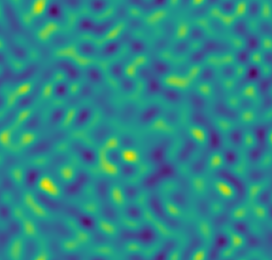
\includegraphics[interpolate=true,width=2.520000in,height=2.380000in]{burgers_solution_0.0-img0.png}}%
\end{pgfscope}%
\begin{pgfscope}%
\pgfsetbuttcap%
\pgfsetroundjoin%
\definecolor{currentfill}{rgb}{0.000000,0.000000,0.000000}%
\pgfsetfillcolor{currentfill}%
\pgfsetlinewidth{0.803000pt}%
\definecolor{currentstroke}{rgb}{0.000000,0.000000,0.000000}%
\pgfsetstrokecolor{currentstroke}%
\pgfsetdash{}{0pt}%
\pgfsys@defobject{currentmarker}{\pgfqpoint{0.000000in}{-0.048611in}}{\pgfqpoint{0.000000in}{0.000000in}}{%
\pgfpathmoveto{\pgfqpoint{0.000000in}{0.000000in}}%
\pgfpathlineto{\pgfqpoint{0.000000in}{-0.048611in}}%
\pgfusepath{stroke,fill}%
}%
\begin{pgfscope}%
\pgfsys@transformshift{0.567820in}{0.517039in}%
\pgfsys@useobject{currentmarker}{}%
\end{pgfscope}%
\end{pgfscope}%
\begin{pgfscope}%
\definecolor{textcolor}{rgb}{0.000000,0.000000,0.000000}%
\pgfsetstrokecolor{textcolor}%
\pgfsetfillcolor{textcolor}%
\pgftext[x=0.567820in,y=0.419816in,,top]{\color{textcolor}{\rmfamily\fontsize{12.000000}{14.400000}\selectfont\catcode`\^=\active\def^{\ifmmode\sp\else\^{}\fi}\catcode`\%=\active\def%{\%}0.0}}%
\end{pgfscope}%
\begin{pgfscope}%
\pgfsetbuttcap%
\pgfsetroundjoin%
\definecolor{currentfill}{rgb}{0.000000,0.000000,0.000000}%
\pgfsetfillcolor{currentfill}%
\pgfsetlinewidth{0.803000pt}%
\definecolor{currentstroke}{rgb}{0.000000,0.000000,0.000000}%
\pgfsetstrokecolor{currentstroke}%
\pgfsetdash{}{0pt}%
\pgfsys@defobject{currentmarker}{\pgfqpoint{0.000000in}{-0.048611in}}{\pgfqpoint{0.000000in}{0.000000in}}{%
\pgfpathmoveto{\pgfqpoint{0.000000in}{0.000000in}}%
\pgfpathlineto{\pgfqpoint{0.000000in}{-0.048611in}}%
\pgfusepath{stroke,fill}%
}%
\begin{pgfscope}%
\pgfsys@transformshift{1.196524in}{0.517039in}%
\pgfsys@useobject{currentmarker}{}%
\end{pgfscope}%
\end{pgfscope}%
\begin{pgfscope}%
\definecolor{textcolor}{rgb}{0.000000,0.000000,0.000000}%
\pgfsetstrokecolor{textcolor}%
\pgfsetfillcolor{textcolor}%
\pgftext[x=1.196524in,y=0.419816in,,top]{\color{textcolor}{\rmfamily\fontsize{12.000000}{14.400000}\selectfont\catcode`\^=\active\def^{\ifmmode\sp\else\^{}\fi}\catcode`\%=\active\def%{\%}0.5}}%
\end{pgfscope}%
\begin{pgfscope}%
\pgfsetbuttcap%
\pgfsetroundjoin%
\definecolor{currentfill}{rgb}{0.000000,0.000000,0.000000}%
\pgfsetfillcolor{currentfill}%
\pgfsetlinewidth{0.803000pt}%
\definecolor{currentstroke}{rgb}{0.000000,0.000000,0.000000}%
\pgfsetstrokecolor{currentstroke}%
\pgfsetdash{}{0pt}%
\pgfsys@defobject{currentmarker}{\pgfqpoint{0.000000in}{-0.048611in}}{\pgfqpoint{0.000000in}{0.000000in}}{%
\pgfpathmoveto{\pgfqpoint{0.000000in}{0.000000in}}%
\pgfpathlineto{\pgfqpoint{0.000000in}{-0.048611in}}%
\pgfusepath{stroke,fill}%
}%
\begin{pgfscope}%
\pgfsys@transformshift{1.825229in}{0.517039in}%
\pgfsys@useobject{currentmarker}{}%
\end{pgfscope}%
\end{pgfscope}%
\begin{pgfscope}%
\definecolor{textcolor}{rgb}{0.000000,0.000000,0.000000}%
\pgfsetstrokecolor{textcolor}%
\pgfsetfillcolor{textcolor}%
\pgftext[x=1.825229in,y=0.419816in,,top]{\color{textcolor}{\rmfamily\fontsize{12.000000}{14.400000}\selectfont\catcode`\^=\active\def^{\ifmmode\sp\else\^{}\fi}\catcode`\%=\active\def%{\%}1.0}}%
\end{pgfscope}%
\begin{pgfscope}%
\pgfsetbuttcap%
\pgfsetroundjoin%
\definecolor{currentfill}{rgb}{0.000000,0.000000,0.000000}%
\pgfsetfillcolor{currentfill}%
\pgfsetlinewidth{0.803000pt}%
\definecolor{currentstroke}{rgb}{0.000000,0.000000,0.000000}%
\pgfsetstrokecolor{currentstroke}%
\pgfsetdash{}{0pt}%
\pgfsys@defobject{currentmarker}{\pgfqpoint{0.000000in}{-0.048611in}}{\pgfqpoint{0.000000in}{0.000000in}}{%
\pgfpathmoveto{\pgfqpoint{0.000000in}{0.000000in}}%
\pgfpathlineto{\pgfqpoint{0.000000in}{-0.048611in}}%
\pgfusepath{stroke,fill}%
}%
\begin{pgfscope}%
\pgfsys@transformshift{2.453933in}{0.517039in}%
\pgfsys@useobject{currentmarker}{}%
\end{pgfscope}%
\end{pgfscope}%
\begin{pgfscope}%
\definecolor{textcolor}{rgb}{0.000000,0.000000,0.000000}%
\pgfsetstrokecolor{textcolor}%
\pgfsetfillcolor{textcolor}%
\pgftext[x=2.453933in,y=0.419816in,,top]{\color{textcolor}{\rmfamily\fontsize{12.000000}{14.400000}\selectfont\catcode`\^=\active\def^{\ifmmode\sp\else\^{}\fi}\catcode`\%=\active\def%{\%}1.5}}%
\end{pgfscope}%
\begin{pgfscope}%
\pgfsetbuttcap%
\pgfsetroundjoin%
\definecolor{currentfill}{rgb}{0.000000,0.000000,0.000000}%
\pgfsetfillcolor{currentfill}%
\pgfsetlinewidth{0.803000pt}%
\definecolor{currentstroke}{rgb}{0.000000,0.000000,0.000000}%
\pgfsetstrokecolor{currentstroke}%
\pgfsetdash{}{0pt}%
\pgfsys@defobject{currentmarker}{\pgfqpoint{0.000000in}{-0.048611in}}{\pgfqpoint{0.000000in}{0.000000in}}{%
\pgfpathmoveto{\pgfqpoint{0.000000in}{0.000000in}}%
\pgfpathlineto{\pgfqpoint{0.000000in}{-0.048611in}}%
\pgfusepath{stroke,fill}%
}%
\begin{pgfscope}%
\pgfsys@transformshift{3.082637in}{0.517039in}%
\pgfsys@useobject{currentmarker}{}%
\end{pgfscope}%
\end{pgfscope}%
\begin{pgfscope}%
\definecolor{textcolor}{rgb}{0.000000,0.000000,0.000000}%
\pgfsetstrokecolor{textcolor}%
\pgfsetfillcolor{textcolor}%
\pgftext[x=3.082637in,y=0.419816in,,top]{\color{textcolor}{\rmfamily\fontsize{12.000000}{14.400000}\selectfont\catcode`\^=\active\def^{\ifmmode\sp\else\^{}\fi}\catcode`\%=\active\def%{\%}2.0}}%
\end{pgfscope}%
\begin{pgfscope}%
\definecolor{textcolor}{rgb}{0.000000,0.000000,0.000000}%
\pgfsetstrokecolor{textcolor}%
\pgfsetfillcolor{textcolor}%
\pgftext[x=1.825229in,y=0.202965in,,top]{\color{textcolor}{\rmfamily\fontsize{12.000000}{14.400000}\selectfont\catcode`\^=\active\def^{\ifmmode\sp\else\^{}\fi}\catcode`\%=\active\def%{\%}Space}}%
\end{pgfscope}%
\begin{pgfscope}%
\pgfsetbuttcap%
\pgfsetroundjoin%
\definecolor{currentfill}{rgb}{0.000000,0.000000,0.000000}%
\pgfsetfillcolor{currentfill}%
\pgfsetlinewidth{0.803000pt}%
\definecolor{currentstroke}{rgb}{0.000000,0.000000,0.000000}%
\pgfsetstrokecolor{currentstroke}%
\pgfsetdash{}{0pt}%
\pgfsys@defobject{currentmarker}{\pgfqpoint{-0.048611in}{0.000000in}}{\pgfqpoint{-0.000000in}{0.000000in}}{%
\pgfpathmoveto{\pgfqpoint{-0.000000in}{0.000000in}}%
\pgfpathlineto{\pgfqpoint{-0.048611in}{0.000000in}}%
\pgfusepath{stroke,fill}%
}%
\begin{pgfscope}%
\pgfsys@transformshift{0.567820in}{0.517039in}%
\pgfsys@useobject{currentmarker}{}%
\end{pgfscope}%
\end{pgfscope}%
\begin{pgfscope}%
\definecolor{textcolor}{rgb}{0.000000,0.000000,0.000000}%
\pgfsetstrokecolor{textcolor}%
\pgfsetfillcolor{textcolor}%
\pgftext[x=0.364559in, y=0.453725in, left, base]{\color{textcolor}{\rmfamily\fontsize{12.000000}{14.400000}\selectfont\catcode`\^=\active\def^{\ifmmode\sp\else\^{}\fi}\catcode`\%=\active\def%{\%}0}}%
\end{pgfscope}%
\begin{pgfscope}%
\pgfsetbuttcap%
\pgfsetroundjoin%
\definecolor{currentfill}{rgb}{0.000000,0.000000,0.000000}%
\pgfsetfillcolor{currentfill}%
\pgfsetlinewidth{0.803000pt}%
\definecolor{currentstroke}{rgb}{0.000000,0.000000,0.000000}%
\pgfsetstrokecolor{currentstroke}%
\pgfsetdash{}{0pt}%
\pgfsys@defobject{currentmarker}{\pgfqpoint{-0.048611in}{0.000000in}}{\pgfqpoint{-0.000000in}{0.000000in}}{%
\pgfpathmoveto{\pgfqpoint{-0.000000in}{0.000000in}}%
\pgfpathlineto{\pgfqpoint{-0.048611in}{0.000000in}}%
\pgfusepath{stroke,fill}%
}%
\begin{pgfscope}%
\pgfsys@transformshift{0.567820in}{0.992634in}%
\pgfsys@useobject{currentmarker}{}%
\end{pgfscope}%
\end{pgfscope}%
\begin{pgfscope}%
\definecolor{textcolor}{rgb}{0.000000,0.000000,0.000000}%
\pgfsetstrokecolor{textcolor}%
\pgfsetfillcolor{textcolor}%
\pgftext[x=0.364559in, y=0.929320in, left, base]{\color{textcolor}{\rmfamily\fontsize{12.000000}{14.400000}\selectfont\catcode`\^=\active\def^{\ifmmode\sp\else\^{}\fi}\catcode`\%=\active\def%{\%}2}}%
\end{pgfscope}%
\begin{pgfscope}%
\pgfsetbuttcap%
\pgfsetroundjoin%
\definecolor{currentfill}{rgb}{0.000000,0.000000,0.000000}%
\pgfsetfillcolor{currentfill}%
\pgfsetlinewidth{0.803000pt}%
\definecolor{currentstroke}{rgb}{0.000000,0.000000,0.000000}%
\pgfsetstrokecolor{currentstroke}%
\pgfsetdash{}{0pt}%
\pgfsys@defobject{currentmarker}{\pgfqpoint{-0.048611in}{0.000000in}}{\pgfqpoint{-0.000000in}{0.000000in}}{%
\pgfpathmoveto{\pgfqpoint{-0.000000in}{0.000000in}}%
\pgfpathlineto{\pgfqpoint{-0.048611in}{0.000000in}}%
\pgfusepath{stroke,fill}%
}%
\begin{pgfscope}%
\pgfsys@transformshift{0.567820in}{1.468230in}%
\pgfsys@useobject{currentmarker}{}%
\end{pgfscope}%
\end{pgfscope}%
\begin{pgfscope}%
\definecolor{textcolor}{rgb}{0.000000,0.000000,0.000000}%
\pgfsetstrokecolor{textcolor}%
\pgfsetfillcolor{textcolor}%
\pgftext[x=0.364559in, y=1.404916in, left, base]{\color{textcolor}{\rmfamily\fontsize{12.000000}{14.400000}\selectfont\catcode`\^=\active\def^{\ifmmode\sp\else\^{}\fi}\catcode`\%=\active\def%{\%}4}}%
\end{pgfscope}%
\begin{pgfscope}%
\pgfsetbuttcap%
\pgfsetroundjoin%
\definecolor{currentfill}{rgb}{0.000000,0.000000,0.000000}%
\pgfsetfillcolor{currentfill}%
\pgfsetlinewidth{0.803000pt}%
\definecolor{currentstroke}{rgb}{0.000000,0.000000,0.000000}%
\pgfsetstrokecolor{currentstroke}%
\pgfsetdash{}{0pt}%
\pgfsys@defobject{currentmarker}{\pgfqpoint{-0.048611in}{0.000000in}}{\pgfqpoint{-0.000000in}{0.000000in}}{%
\pgfpathmoveto{\pgfqpoint{-0.000000in}{0.000000in}}%
\pgfpathlineto{\pgfqpoint{-0.048611in}{0.000000in}}%
\pgfusepath{stroke,fill}%
}%
\begin{pgfscope}%
\pgfsys@transformshift{0.567820in}{1.943825in}%
\pgfsys@useobject{currentmarker}{}%
\end{pgfscope}%
\end{pgfscope}%
\begin{pgfscope}%
\definecolor{textcolor}{rgb}{0.000000,0.000000,0.000000}%
\pgfsetstrokecolor{textcolor}%
\pgfsetfillcolor{textcolor}%
\pgftext[x=0.364559in, y=1.880511in, left, base]{\color{textcolor}{\rmfamily\fontsize{12.000000}{14.400000}\selectfont\catcode`\^=\active\def^{\ifmmode\sp\else\^{}\fi}\catcode`\%=\active\def%{\%}6}}%
\end{pgfscope}%
\begin{pgfscope}%
\pgfsetbuttcap%
\pgfsetroundjoin%
\definecolor{currentfill}{rgb}{0.000000,0.000000,0.000000}%
\pgfsetfillcolor{currentfill}%
\pgfsetlinewidth{0.803000pt}%
\definecolor{currentstroke}{rgb}{0.000000,0.000000,0.000000}%
\pgfsetstrokecolor{currentstroke}%
\pgfsetdash{}{0pt}%
\pgfsys@defobject{currentmarker}{\pgfqpoint{-0.048611in}{0.000000in}}{\pgfqpoint{-0.000000in}{0.000000in}}{%
\pgfpathmoveto{\pgfqpoint{-0.000000in}{0.000000in}}%
\pgfpathlineto{\pgfqpoint{-0.048611in}{0.000000in}}%
\pgfusepath{stroke,fill}%
}%
\begin{pgfscope}%
\pgfsys@transformshift{0.567820in}{2.419421in}%
\pgfsys@useobject{currentmarker}{}%
\end{pgfscope}%
\end{pgfscope}%
\begin{pgfscope}%
\definecolor{textcolor}{rgb}{0.000000,0.000000,0.000000}%
\pgfsetstrokecolor{textcolor}%
\pgfsetfillcolor{textcolor}%
\pgftext[x=0.364559in, y=2.356107in, left, base]{\color{textcolor}{\rmfamily\fontsize{12.000000}{14.400000}\selectfont\catcode`\^=\active\def^{\ifmmode\sp\else\^{}\fi}\catcode`\%=\active\def%{\%}8}}%
\end{pgfscope}%
\begin{pgfscope}%
\pgfsetbuttcap%
\pgfsetroundjoin%
\definecolor{currentfill}{rgb}{0.000000,0.000000,0.000000}%
\pgfsetfillcolor{currentfill}%
\pgfsetlinewidth{0.803000pt}%
\definecolor{currentstroke}{rgb}{0.000000,0.000000,0.000000}%
\pgfsetstrokecolor{currentstroke}%
\pgfsetdash{}{0pt}%
\pgfsys@defobject{currentmarker}{\pgfqpoint{-0.048611in}{0.000000in}}{\pgfqpoint{-0.000000in}{0.000000in}}{%
\pgfpathmoveto{\pgfqpoint{-0.000000in}{0.000000in}}%
\pgfpathlineto{\pgfqpoint{-0.048611in}{0.000000in}}%
\pgfusepath{stroke,fill}%
}%
\begin{pgfscope}%
\pgfsys@transformshift{0.567820in}{2.895016in}%
\pgfsys@useobject{currentmarker}{}%
\end{pgfscope}%
\end{pgfscope}%
\begin{pgfscope}%
\definecolor{textcolor}{rgb}{0.000000,0.000000,0.000000}%
\pgfsetstrokecolor{textcolor}%
\pgfsetfillcolor{textcolor}%
\pgftext[x=0.258521in, y=2.831702in, left, base]{\color{textcolor}{\rmfamily\fontsize{12.000000}{14.400000}\selectfont\catcode`\^=\active\def^{\ifmmode\sp\else\^{}\fi}\catcode`\%=\active\def%{\%}10}}%
\end{pgfscope}%
\begin{pgfscope}%
\definecolor{textcolor}{rgb}{0.000000,0.000000,0.000000}%
\pgfsetstrokecolor{textcolor}%
\pgfsetfillcolor{textcolor}%
\pgftext[x=0.202965in,y=1.706027in,,bottom,rotate=90.000000]{\color{textcolor}{\rmfamily\fontsize{12.000000}{14.400000}\selectfont\catcode`\^=\active\def^{\ifmmode\sp\else\^{}\fi}\catcode`\%=\active\def%{\%}Time}}%
\end{pgfscope}%
\begin{pgfscope}%
\pgfsetrectcap%
\pgfsetmiterjoin%
\pgfsetlinewidth{0.803000pt}%
\definecolor{currentstroke}{rgb}{0.000000,0.000000,0.000000}%
\pgfsetstrokecolor{currentstroke}%
\pgfsetdash{}{0pt}%
\pgfpathmoveto{\pgfqpoint{0.567820in}{0.517039in}}%
\pgfpathlineto{\pgfqpoint{0.567820in}{2.895016in}}%
\pgfusepath{stroke}%
\end{pgfscope}%
\begin{pgfscope}%
\pgfsetrectcap%
\pgfsetmiterjoin%
\pgfsetlinewidth{0.803000pt}%
\definecolor{currentstroke}{rgb}{0.000000,0.000000,0.000000}%
\pgfsetstrokecolor{currentstroke}%
\pgfsetdash{}{0pt}%
\pgfpathmoveto{\pgfqpoint{3.082637in}{0.517039in}}%
\pgfpathlineto{\pgfqpoint{3.082637in}{2.895016in}}%
\pgfusepath{stroke}%
\end{pgfscope}%
\begin{pgfscope}%
\pgfsetrectcap%
\pgfsetmiterjoin%
\pgfsetlinewidth{0.803000pt}%
\definecolor{currentstroke}{rgb}{0.000000,0.000000,0.000000}%
\pgfsetstrokecolor{currentstroke}%
\pgfsetdash{}{0pt}%
\pgfpathmoveto{\pgfqpoint{0.567820in}{0.517039in}}%
\pgfpathlineto{\pgfqpoint{3.082637in}{0.517039in}}%
\pgfusepath{stroke}%
\end{pgfscope}%
\begin{pgfscope}%
\pgfsetrectcap%
\pgfsetmiterjoin%
\pgfsetlinewidth{0.803000pt}%
\definecolor{currentstroke}{rgb}{0.000000,0.000000,0.000000}%
\pgfsetstrokecolor{currentstroke}%
\pgfsetdash{}{0pt}%
\pgfpathmoveto{\pgfqpoint{0.567820in}{2.895016in}}%
\pgfpathlineto{\pgfqpoint{3.082637in}{2.895016in}}%
\pgfusepath{stroke}%
\end{pgfscope}%
\begin{pgfscope}%
\pgfsetbuttcap%
\pgfsetmiterjoin%
\pgfsetlinewidth{0.000000pt}%
\definecolor{currentstroke}{rgb}{0.000000,0.000000,0.000000}%
\pgfsetstrokecolor{currentstroke}%
\pgfsetstrokeopacity{0.000000}%
\pgfsetdash{}{0pt}%
\pgfpathmoveto{\pgfqpoint{3.340906in}{0.517039in}}%
\pgfpathlineto{\pgfqpoint{3.459805in}{0.517039in}}%
\pgfpathlineto{\pgfqpoint{3.459805in}{2.895016in}}%
\pgfpathlineto{\pgfqpoint{3.340906in}{2.895016in}}%
\pgfpathlineto{\pgfqpoint{3.340906in}{0.517039in}}%
\pgfpathclose%
\pgfusepath{}%
\end{pgfscope}%
\begin{pgfscope}%
\pgfsys@transformshift{3.340000in}{0.520000in}%
\pgftext[left,bottom]{
\includegraphics[interpolate=true,width=0.120000in,height=2.380000in]{burgers_solution_0.0-img1.png}}%
\end{pgfscope}%
\begin{pgfscope}%
\pgfsetbuttcap%
\pgfsetroundjoin%
\definecolor{currentfill}{rgb}{0.000000,0.000000,0.000000}%
\pgfsetfillcolor{currentfill}%
\pgfsetlinewidth{0.803000pt}%
\definecolor{currentstroke}{rgb}{0.000000,0.000000,0.000000}%
\pgfsetstrokecolor{currentstroke}%
\pgfsetdash{}{0pt}%
\pgfsys@defobject{currentmarker}{\pgfqpoint{0.000000in}{0.000000in}}{\pgfqpoint{0.048611in}{0.000000in}}{%
\pgfpathmoveto{\pgfqpoint{0.000000in}{0.000000in}}%
\pgfpathlineto{\pgfqpoint{0.048611in}{0.000000in}}%
\pgfusepath{stroke,fill}%
}%
\begin{pgfscope}%
\pgfsys@transformshift{3.459805in}{0.555741in}%
\pgfsys@useobject{currentmarker}{}%
\end{pgfscope}%
\end{pgfscope}%
\begin{pgfscope}%
\definecolor{textcolor}{rgb}{0.000000,0.000000,0.000000}%
\pgfsetstrokecolor{textcolor}%
\pgfsetfillcolor{textcolor}%
\pgftext[x=3.557027in, y=0.492427in, left, base]{\color{textcolor}{\rmfamily\fontsize{12.000000}{14.400000}\selectfont\catcode`\^=\active\def^{\ifmmode\sp\else\^{}\fi}\catcode`\%=\active\def%{\%}\ensuremath{-}0.6}}%
\end{pgfscope}%
\begin{pgfscope}%
\pgfsetbuttcap%
\pgfsetroundjoin%
\definecolor{currentfill}{rgb}{0.000000,0.000000,0.000000}%
\pgfsetfillcolor{currentfill}%
\pgfsetlinewidth{0.803000pt}%
\definecolor{currentstroke}{rgb}{0.000000,0.000000,0.000000}%
\pgfsetstrokecolor{currentstroke}%
\pgfsetdash{}{0pt}%
\pgfsys@defobject{currentmarker}{\pgfqpoint{0.000000in}{0.000000in}}{\pgfqpoint{0.048611in}{0.000000in}}{%
\pgfpathmoveto{\pgfqpoint{0.000000in}{0.000000in}}%
\pgfpathlineto{\pgfqpoint{0.048611in}{0.000000in}}%
\pgfusepath{stroke,fill}%
}%
\begin{pgfscope}%
\pgfsys@transformshift{3.459805in}{0.932008in}%
\pgfsys@useobject{currentmarker}{}%
\end{pgfscope}%
\end{pgfscope}%
\begin{pgfscope}%
\definecolor{textcolor}{rgb}{0.000000,0.000000,0.000000}%
\pgfsetstrokecolor{textcolor}%
\pgfsetfillcolor{textcolor}%
\pgftext[x=3.557027in, y=0.868694in, left, base]{\color{textcolor}{\rmfamily\fontsize{12.000000}{14.400000}\selectfont\catcode`\^=\active\def^{\ifmmode\sp\else\^{}\fi}\catcode`\%=\active\def%{\%}\ensuremath{-}0.4}}%
\end{pgfscope}%
\begin{pgfscope}%
\pgfsetbuttcap%
\pgfsetroundjoin%
\definecolor{currentfill}{rgb}{0.000000,0.000000,0.000000}%
\pgfsetfillcolor{currentfill}%
\pgfsetlinewidth{0.803000pt}%
\definecolor{currentstroke}{rgb}{0.000000,0.000000,0.000000}%
\pgfsetstrokecolor{currentstroke}%
\pgfsetdash{}{0pt}%
\pgfsys@defobject{currentmarker}{\pgfqpoint{0.000000in}{0.000000in}}{\pgfqpoint{0.048611in}{0.000000in}}{%
\pgfpathmoveto{\pgfqpoint{0.000000in}{0.000000in}}%
\pgfpathlineto{\pgfqpoint{0.048611in}{0.000000in}}%
\pgfusepath{stroke,fill}%
}%
\begin{pgfscope}%
\pgfsys@transformshift{3.459805in}{1.308274in}%
\pgfsys@useobject{currentmarker}{}%
\end{pgfscope}%
\end{pgfscope}%
\begin{pgfscope}%
\definecolor{textcolor}{rgb}{0.000000,0.000000,0.000000}%
\pgfsetstrokecolor{textcolor}%
\pgfsetfillcolor{textcolor}%
\pgftext[x=3.557027in, y=1.244961in, left, base]{\color{textcolor}{\rmfamily\fontsize{12.000000}{14.400000}\selectfont\catcode`\^=\active\def^{\ifmmode\sp\else\^{}\fi}\catcode`\%=\active\def%{\%}\ensuremath{-}0.2}}%
\end{pgfscope}%
\begin{pgfscope}%
\pgfsetbuttcap%
\pgfsetroundjoin%
\definecolor{currentfill}{rgb}{0.000000,0.000000,0.000000}%
\pgfsetfillcolor{currentfill}%
\pgfsetlinewidth{0.803000pt}%
\definecolor{currentstroke}{rgb}{0.000000,0.000000,0.000000}%
\pgfsetstrokecolor{currentstroke}%
\pgfsetdash{}{0pt}%
\pgfsys@defobject{currentmarker}{\pgfqpoint{0.000000in}{0.000000in}}{\pgfqpoint{0.048611in}{0.000000in}}{%
\pgfpathmoveto{\pgfqpoint{0.000000in}{0.000000in}}%
\pgfpathlineto{\pgfqpoint{0.048611in}{0.000000in}}%
\pgfusepath{stroke,fill}%
}%
\begin{pgfscope}%
\pgfsys@transformshift{3.459805in}{1.684541in}%
\pgfsys@useobject{currentmarker}{}%
\end{pgfscope}%
\end{pgfscope}%
\begin{pgfscope}%
\definecolor{textcolor}{rgb}{0.000000,0.000000,0.000000}%
\pgfsetstrokecolor{textcolor}%
\pgfsetfillcolor{textcolor}%
\pgftext[x=3.557027in, y=1.621228in, left, base]{\color{textcolor}{\rmfamily\fontsize{12.000000}{14.400000}\selectfont\catcode`\^=\active\def^{\ifmmode\sp\else\^{}\fi}\catcode`\%=\active\def%{\%}0.0}}%
\end{pgfscope}%
\begin{pgfscope}%
\pgfsetbuttcap%
\pgfsetroundjoin%
\definecolor{currentfill}{rgb}{0.000000,0.000000,0.000000}%
\pgfsetfillcolor{currentfill}%
\pgfsetlinewidth{0.803000pt}%
\definecolor{currentstroke}{rgb}{0.000000,0.000000,0.000000}%
\pgfsetstrokecolor{currentstroke}%
\pgfsetdash{}{0pt}%
\pgfsys@defobject{currentmarker}{\pgfqpoint{0.000000in}{0.000000in}}{\pgfqpoint{0.048611in}{0.000000in}}{%
\pgfpathmoveto{\pgfqpoint{0.000000in}{0.000000in}}%
\pgfpathlineto{\pgfqpoint{0.048611in}{0.000000in}}%
\pgfusepath{stroke,fill}%
}%
\begin{pgfscope}%
\pgfsys@transformshift{3.459805in}{2.060808in}%
\pgfsys@useobject{currentmarker}{}%
\end{pgfscope}%
\end{pgfscope}%
\begin{pgfscope}%
\definecolor{textcolor}{rgb}{0.000000,0.000000,0.000000}%
\pgfsetstrokecolor{textcolor}%
\pgfsetfillcolor{textcolor}%
\pgftext[x=3.557027in, y=1.997494in, left, base]{\color{textcolor}{\rmfamily\fontsize{12.000000}{14.400000}\selectfont\catcode`\^=\active\def^{\ifmmode\sp\else\^{}\fi}\catcode`\%=\active\def%{\%}0.2}}%
\end{pgfscope}%
\begin{pgfscope}%
\pgfsetbuttcap%
\pgfsetroundjoin%
\definecolor{currentfill}{rgb}{0.000000,0.000000,0.000000}%
\pgfsetfillcolor{currentfill}%
\pgfsetlinewidth{0.803000pt}%
\definecolor{currentstroke}{rgb}{0.000000,0.000000,0.000000}%
\pgfsetstrokecolor{currentstroke}%
\pgfsetdash{}{0pt}%
\pgfsys@defobject{currentmarker}{\pgfqpoint{0.000000in}{0.000000in}}{\pgfqpoint{0.048611in}{0.000000in}}{%
\pgfpathmoveto{\pgfqpoint{0.000000in}{0.000000in}}%
\pgfpathlineto{\pgfqpoint{0.048611in}{0.000000in}}%
\pgfusepath{stroke,fill}%
}%
\begin{pgfscope}%
\pgfsys@transformshift{3.459805in}{2.437075in}%
\pgfsys@useobject{currentmarker}{}%
\end{pgfscope}%
\end{pgfscope}%
\begin{pgfscope}%
\definecolor{textcolor}{rgb}{0.000000,0.000000,0.000000}%
\pgfsetstrokecolor{textcolor}%
\pgfsetfillcolor{textcolor}%
\pgftext[x=3.557027in, y=2.373761in, left, base]{\color{textcolor}{\rmfamily\fontsize{12.000000}{14.400000}\selectfont\catcode`\^=\active\def^{\ifmmode\sp\else\^{}\fi}\catcode`\%=\active\def%{\%}0.4}}%
\end{pgfscope}%
\begin{pgfscope}%
\pgfsetbuttcap%
\pgfsetroundjoin%
\definecolor{currentfill}{rgb}{0.000000,0.000000,0.000000}%
\pgfsetfillcolor{currentfill}%
\pgfsetlinewidth{0.803000pt}%
\definecolor{currentstroke}{rgb}{0.000000,0.000000,0.000000}%
\pgfsetstrokecolor{currentstroke}%
\pgfsetdash{}{0pt}%
\pgfsys@defobject{currentmarker}{\pgfqpoint{0.000000in}{0.000000in}}{\pgfqpoint{0.048611in}{0.000000in}}{%
\pgfpathmoveto{\pgfqpoint{0.000000in}{0.000000in}}%
\pgfpathlineto{\pgfqpoint{0.048611in}{0.000000in}}%
\pgfusepath{stroke,fill}%
}%
\begin{pgfscope}%
\pgfsys@transformshift{3.459805in}{2.813342in}%
\pgfsys@useobject{currentmarker}{}%
\end{pgfscope}%
\end{pgfscope}%
\begin{pgfscope}%
\definecolor{textcolor}{rgb}{0.000000,0.000000,0.000000}%
\pgfsetstrokecolor{textcolor}%
\pgfsetfillcolor{textcolor}%
\pgftext[x=3.557027in, y=2.750028in, left, base]{\color{textcolor}{\rmfamily\fontsize{12.000000}{14.400000}\selectfont\catcode`\^=\active\def^{\ifmmode\sp\else\^{}\fi}\catcode`\%=\active\def%{\%}0.6}}%
\end{pgfscope}%
\begin{pgfscope}%
\pgfsetrectcap%
\pgfsetmiterjoin%
\pgfsetlinewidth{0.803000pt}%
\definecolor{currentstroke}{rgb}{0.000000,0.000000,0.000000}%
\pgfsetstrokecolor{currentstroke}%
\pgfsetdash{}{0pt}%
\pgfpathmoveto{\pgfqpoint{3.340906in}{0.517039in}}%
\pgfpathlineto{\pgfqpoint{3.400355in}{0.517039in}}%
\pgfpathlineto{\pgfqpoint{3.459805in}{0.517039in}}%
\pgfpathlineto{\pgfqpoint{3.459805in}{2.895016in}}%
\pgfpathlineto{\pgfqpoint{3.400355in}{2.895016in}}%
\pgfpathlineto{\pgfqpoint{3.340906in}{2.895016in}}%
\pgfpathlineto{\pgfqpoint{3.340906in}{0.517039in}}%
\pgfpathclose%
\pgfusepath{stroke}%
\end{pgfscope}%
\end{pgfpicture}%
\makeatother%
\endgroup%

    \end{adjustbox}
    \caption{Solution function for \(\nu=0\).}\label{fig:burgers_solution_0.0}
  \end{subfigure}
  \begin{subfigure}{0.49\linewidth}
    \begin{adjustbox}{width=\linewidth}
      \begingroup%
\makeatletter%
\begin{pgfpicture}%
\pgfpathrectangle{\pgfpointorigin}{\pgfqpoint{4.000000in}{3.000000in}}%
\pgfusepath{use as bounding box, clip}%
\begin{pgfscope}%
\pgfsetbuttcap%
\pgfsetmiterjoin%
\pgfsetlinewidth{0.000000pt}%
\definecolor{currentstroke}{rgb}{0.000000,0.000000,0.000000}%
\pgfsetstrokecolor{currentstroke}%
\pgfsetstrokeopacity{0.000000}%
\pgfsetdash{}{0pt}%
\pgfpathmoveto{\pgfqpoint{0.000000in}{0.000000in}}%
\pgfpathlineto{\pgfqpoint{4.000000in}{0.000000in}}%
\pgfpathlineto{\pgfqpoint{4.000000in}{3.000000in}}%
\pgfpathlineto{\pgfqpoint{0.000000in}{3.000000in}}%
\pgfpathlineto{\pgfqpoint{0.000000in}{0.000000in}}%
\pgfpathclose%
\pgfusepath{}%
\end{pgfscope}%
\begin{pgfscope}%
\pgfsetbuttcap%
\pgfsetmiterjoin%
\pgfsetlinewidth{0.000000pt}%
\definecolor{currentstroke}{rgb}{0.000000,0.000000,0.000000}%
\pgfsetstrokecolor{currentstroke}%
\pgfsetstrokeopacity{0.000000}%
\pgfsetdash{}{0pt}%
\pgfpathmoveto{\pgfqpoint{0.567820in}{0.517039in}}%
\pgfpathlineto{\pgfqpoint{3.082637in}{0.517039in}}%
\pgfpathlineto{\pgfqpoint{3.082637in}{2.895016in}}%
\pgfpathlineto{\pgfqpoint{0.567820in}{2.895016in}}%
\pgfpathlineto{\pgfqpoint{0.567820in}{0.517039in}}%
\pgfpathclose%
\pgfusepath{}%
\end{pgfscope}%
\begin{pgfscope}%
\pgfpathrectangle{\pgfqpoint{0.567820in}{0.517039in}}{\pgfqpoint{2.514817in}{2.377978in}}%
\pgfusepath{clip}%
\pgfsys@transformshift{0.567820in}{0.517039in}%
\pgftext[left,bottom]{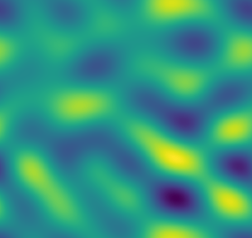
\includegraphics[interpolate=true,width=2.520000in,height=2.380000in]{burgers_forcing_0.0-img0.png}}%
\end{pgfscope}%
\begin{pgfscope}%
\pgfsetbuttcap%
\pgfsetroundjoin%
\definecolor{currentfill}{rgb}{0.000000,0.000000,0.000000}%
\pgfsetfillcolor{currentfill}%
\pgfsetlinewidth{0.803000pt}%
\definecolor{currentstroke}{rgb}{0.000000,0.000000,0.000000}%
\pgfsetstrokecolor{currentstroke}%
\pgfsetdash{}{0pt}%
\pgfsys@defobject{currentmarker}{\pgfqpoint{0.000000in}{-0.048611in}}{\pgfqpoint{0.000000in}{0.000000in}}{%
\pgfpathmoveto{\pgfqpoint{0.000000in}{0.000000in}}%
\pgfpathlineto{\pgfqpoint{0.000000in}{-0.048611in}}%
\pgfusepath{stroke,fill}%
}%
\begin{pgfscope}%
\pgfsys@transformshift{0.567820in}{0.517039in}%
\pgfsys@useobject{currentmarker}{}%
\end{pgfscope}%
\end{pgfscope}%
\begin{pgfscope}%
\definecolor{textcolor}{rgb}{0.000000,0.000000,0.000000}%
\pgfsetstrokecolor{textcolor}%
\pgfsetfillcolor{textcolor}%
\pgftext[x=0.567820in,y=0.419816in,,top]{\color{textcolor}{\rmfamily\fontsize{12.000000}{14.400000}\selectfont\catcode`\^=\active\def^{\ifmmode\sp\else\^{}\fi}\catcode`\%=\active\def%{\%}0.0}}%
\end{pgfscope}%
\begin{pgfscope}%
\pgfsetbuttcap%
\pgfsetroundjoin%
\definecolor{currentfill}{rgb}{0.000000,0.000000,0.000000}%
\pgfsetfillcolor{currentfill}%
\pgfsetlinewidth{0.803000pt}%
\definecolor{currentstroke}{rgb}{0.000000,0.000000,0.000000}%
\pgfsetstrokecolor{currentstroke}%
\pgfsetdash{}{0pt}%
\pgfsys@defobject{currentmarker}{\pgfqpoint{0.000000in}{-0.048611in}}{\pgfqpoint{0.000000in}{0.000000in}}{%
\pgfpathmoveto{\pgfqpoint{0.000000in}{0.000000in}}%
\pgfpathlineto{\pgfqpoint{0.000000in}{-0.048611in}}%
\pgfusepath{stroke,fill}%
}%
\begin{pgfscope}%
\pgfsys@transformshift{1.196524in}{0.517039in}%
\pgfsys@useobject{currentmarker}{}%
\end{pgfscope}%
\end{pgfscope}%
\begin{pgfscope}%
\definecolor{textcolor}{rgb}{0.000000,0.000000,0.000000}%
\pgfsetstrokecolor{textcolor}%
\pgfsetfillcolor{textcolor}%
\pgftext[x=1.196524in,y=0.419816in,,top]{\color{textcolor}{\rmfamily\fontsize{12.000000}{14.400000}\selectfont\catcode`\^=\active\def^{\ifmmode\sp\else\^{}\fi}\catcode`\%=\active\def%{\%}0.5}}%
\end{pgfscope}%
\begin{pgfscope}%
\pgfsetbuttcap%
\pgfsetroundjoin%
\definecolor{currentfill}{rgb}{0.000000,0.000000,0.000000}%
\pgfsetfillcolor{currentfill}%
\pgfsetlinewidth{0.803000pt}%
\definecolor{currentstroke}{rgb}{0.000000,0.000000,0.000000}%
\pgfsetstrokecolor{currentstroke}%
\pgfsetdash{}{0pt}%
\pgfsys@defobject{currentmarker}{\pgfqpoint{0.000000in}{-0.048611in}}{\pgfqpoint{0.000000in}{0.000000in}}{%
\pgfpathmoveto{\pgfqpoint{0.000000in}{0.000000in}}%
\pgfpathlineto{\pgfqpoint{0.000000in}{-0.048611in}}%
\pgfusepath{stroke,fill}%
}%
\begin{pgfscope}%
\pgfsys@transformshift{1.825229in}{0.517039in}%
\pgfsys@useobject{currentmarker}{}%
\end{pgfscope}%
\end{pgfscope}%
\begin{pgfscope}%
\definecolor{textcolor}{rgb}{0.000000,0.000000,0.000000}%
\pgfsetstrokecolor{textcolor}%
\pgfsetfillcolor{textcolor}%
\pgftext[x=1.825229in,y=0.419816in,,top]{\color{textcolor}{\rmfamily\fontsize{12.000000}{14.400000}\selectfont\catcode`\^=\active\def^{\ifmmode\sp\else\^{}\fi}\catcode`\%=\active\def%{\%}1.0}}%
\end{pgfscope}%
\begin{pgfscope}%
\pgfsetbuttcap%
\pgfsetroundjoin%
\definecolor{currentfill}{rgb}{0.000000,0.000000,0.000000}%
\pgfsetfillcolor{currentfill}%
\pgfsetlinewidth{0.803000pt}%
\definecolor{currentstroke}{rgb}{0.000000,0.000000,0.000000}%
\pgfsetstrokecolor{currentstroke}%
\pgfsetdash{}{0pt}%
\pgfsys@defobject{currentmarker}{\pgfqpoint{0.000000in}{-0.048611in}}{\pgfqpoint{0.000000in}{0.000000in}}{%
\pgfpathmoveto{\pgfqpoint{0.000000in}{0.000000in}}%
\pgfpathlineto{\pgfqpoint{0.000000in}{-0.048611in}}%
\pgfusepath{stroke,fill}%
}%
\begin{pgfscope}%
\pgfsys@transformshift{2.453933in}{0.517039in}%
\pgfsys@useobject{currentmarker}{}%
\end{pgfscope}%
\end{pgfscope}%
\begin{pgfscope}%
\definecolor{textcolor}{rgb}{0.000000,0.000000,0.000000}%
\pgfsetstrokecolor{textcolor}%
\pgfsetfillcolor{textcolor}%
\pgftext[x=2.453933in,y=0.419816in,,top]{\color{textcolor}{\rmfamily\fontsize{12.000000}{14.400000}\selectfont\catcode`\^=\active\def^{\ifmmode\sp\else\^{}\fi}\catcode`\%=\active\def%{\%}1.5}}%
\end{pgfscope}%
\begin{pgfscope}%
\pgfsetbuttcap%
\pgfsetroundjoin%
\definecolor{currentfill}{rgb}{0.000000,0.000000,0.000000}%
\pgfsetfillcolor{currentfill}%
\pgfsetlinewidth{0.803000pt}%
\definecolor{currentstroke}{rgb}{0.000000,0.000000,0.000000}%
\pgfsetstrokecolor{currentstroke}%
\pgfsetdash{}{0pt}%
\pgfsys@defobject{currentmarker}{\pgfqpoint{0.000000in}{-0.048611in}}{\pgfqpoint{0.000000in}{0.000000in}}{%
\pgfpathmoveto{\pgfqpoint{0.000000in}{0.000000in}}%
\pgfpathlineto{\pgfqpoint{0.000000in}{-0.048611in}}%
\pgfusepath{stroke,fill}%
}%
\begin{pgfscope}%
\pgfsys@transformshift{3.082637in}{0.517039in}%
\pgfsys@useobject{currentmarker}{}%
\end{pgfscope}%
\end{pgfscope}%
\begin{pgfscope}%
\definecolor{textcolor}{rgb}{0.000000,0.000000,0.000000}%
\pgfsetstrokecolor{textcolor}%
\pgfsetfillcolor{textcolor}%
\pgftext[x=3.082637in,y=0.419816in,,top]{\color{textcolor}{\rmfamily\fontsize{12.000000}{14.400000}\selectfont\catcode`\^=\active\def^{\ifmmode\sp\else\^{}\fi}\catcode`\%=\active\def%{\%}2.0}}%
\end{pgfscope}%
\begin{pgfscope}%
\definecolor{textcolor}{rgb}{0.000000,0.000000,0.000000}%
\pgfsetstrokecolor{textcolor}%
\pgfsetfillcolor{textcolor}%
\pgftext[x=1.825229in,y=0.202965in,,top]{\color{textcolor}{\rmfamily\fontsize{12.000000}{14.400000}\selectfont\catcode`\^=\active\def^{\ifmmode\sp\else\^{}\fi}\catcode`\%=\active\def%{\%}Space}}%
\end{pgfscope}%
\begin{pgfscope}%
\pgfsetbuttcap%
\pgfsetroundjoin%
\definecolor{currentfill}{rgb}{0.000000,0.000000,0.000000}%
\pgfsetfillcolor{currentfill}%
\pgfsetlinewidth{0.803000pt}%
\definecolor{currentstroke}{rgb}{0.000000,0.000000,0.000000}%
\pgfsetstrokecolor{currentstroke}%
\pgfsetdash{}{0pt}%
\pgfsys@defobject{currentmarker}{\pgfqpoint{-0.048611in}{0.000000in}}{\pgfqpoint{-0.000000in}{0.000000in}}{%
\pgfpathmoveto{\pgfqpoint{-0.000000in}{0.000000in}}%
\pgfpathlineto{\pgfqpoint{-0.048611in}{0.000000in}}%
\pgfusepath{stroke,fill}%
}%
\begin{pgfscope}%
\pgfsys@transformshift{0.567820in}{0.517039in}%
\pgfsys@useobject{currentmarker}{}%
\end{pgfscope}%
\end{pgfscope}%
\begin{pgfscope}%
\definecolor{textcolor}{rgb}{0.000000,0.000000,0.000000}%
\pgfsetstrokecolor{textcolor}%
\pgfsetfillcolor{textcolor}%
\pgftext[x=0.364559in, y=0.453725in, left, base]{\color{textcolor}{\rmfamily\fontsize{12.000000}{14.400000}\selectfont\catcode`\^=\active\def^{\ifmmode\sp\else\^{}\fi}\catcode`\%=\active\def%{\%}0}}%
\end{pgfscope}%
\begin{pgfscope}%
\pgfsetbuttcap%
\pgfsetroundjoin%
\definecolor{currentfill}{rgb}{0.000000,0.000000,0.000000}%
\pgfsetfillcolor{currentfill}%
\pgfsetlinewidth{0.803000pt}%
\definecolor{currentstroke}{rgb}{0.000000,0.000000,0.000000}%
\pgfsetstrokecolor{currentstroke}%
\pgfsetdash{}{0pt}%
\pgfsys@defobject{currentmarker}{\pgfqpoint{-0.048611in}{0.000000in}}{\pgfqpoint{-0.000000in}{0.000000in}}{%
\pgfpathmoveto{\pgfqpoint{-0.000000in}{0.000000in}}%
\pgfpathlineto{\pgfqpoint{-0.048611in}{0.000000in}}%
\pgfusepath{stroke,fill}%
}%
\begin{pgfscope}%
\pgfsys@transformshift{0.567820in}{0.992634in}%
\pgfsys@useobject{currentmarker}{}%
\end{pgfscope}%
\end{pgfscope}%
\begin{pgfscope}%
\definecolor{textcolor}{rgb}{0.000000,0.000000,0.000000}%
\pgfsetstrokecolor{textcolor}%
\pgfsetfillcolor{textcolor}%
\pgftext[x=0.364559in, y=0.929320in, left, base]{\color{textcolor}{\rmfamily\fontsize{12.000000}{14.400000}\selectfont\catcode`\^=\active\def^{\ifmmode\sp\else\^{}\fi}\catcode`\%=\active\def%{\%}2}}%
\end{pgfscope}%
\begin{pgfscope}%
\pgfsetbuttcap%
\pgfsetroundjoin%
\definecolor{currentfill}{rgb}{0.000000,0.000000,0.000000}%
\pgfsetfillcolor{currentfill}%
\pgfsetlinewidth{0.803000pt}%
\definecolor{currentstroke}{rgb}{0.000000,0.000000,0.000000}%
\pgfsetstrokecolor{currentstroke}%
\pgfsetdash{}{0pt}%
\pgfsys@defobject{currentmarker}{\pgfqpoint{-0.048611in}{0.000000in}}{\pgfqpoint{-0.000000in}{0.000000in}}{%
\pgfpathmoveto{\pgfqpoint{-0.000000in}{0.000000in}}%
\pgfpathlineto{\pgfqpoint{-0.048611in}{0.000000in}}%
\pgfusepath{stroke,fill}%
}%
\begin{pgfscope}%
\pgfsys@transformshift{0.567820in}{1.468230in}%
\pgfsys@useobject{currentmarker}{}%
\end{pgfscope}%
\end{pgfscope}%
\begin{pgfscope}%
\definecolor{textcolor}{rgb}{0.000000,0.000000,0.000000}%
\pgfsetstrokecolor{textcolor}%
\pgfsetfillcolor{textcolor}%
\pgftext[x=0.364559in, y=1.404916in, left, base]{\color{textcolor}{\rmfamily\fontsize{12.000000}{14.400000}\selectfont\catcode`\^=\active\def^{\ifmmode\sp\else\^{}\fi}\catcode`\%=\active\def%{\%}4}}%
\end{pgfscope}%
\begin{pgfscope}%
\pgfsetbuttcap%
\pgfsetroundjoin%
\definecolor{currentfill}{rgb}{0.000000,0.000000,0.000000}%
\pgfsetfillcolor{currentfill}%
\pgfsetlinewidth{0.803000pt}%
\definecolor{currentstroke}{rgb}{0.000000,0.000000,0.000000}%
\pgfsetstrokecolor{currentstroke}%
\pgfsetdash{}{0pt}%
\pgfsys@defobject{currentmarker}{\pgfqpoint{-0.048611in}{0.000000in}}{\pgfqpoint{-0.000000in}{0.000000in}}{%
\pgfpathmoveto{\pgfqpoint{-0.000000in}{0.000000in}}%
\pgfpathlineto{\pgfqpoint{-0.048611in}{0.000000in}}%
\pgfusepath{stroke,fill}%
}%
\begin{pgfscope}%
\pgfsys@transformshift{0.567820in}{1.943825in}%
\pgfsys@useobject{currentmarker}{}%
\end{pgfscope}%
\end{pgfscope}%
\begin{pgfscope}%
\definecolor{textcolor}{rgb}{0.000000,0.000000,0.000000}%
\pgfsetstrokecolor{textcolor}%
\pgfsetfillcolor{textcolor}%
\pgftext[x=0.364559in, y=1.880511in, left, base]{\color{textcolor}{\rmfamily\fontsize{12.000000}{14.400000}\selectfont\catcode`\^=\active\def^{\ifmmode\sp\else\^{}\fi}\catcode`\%=\active\def%{\%}6}}%
\end{pgfscope}%
\begin{pgfscope}%
\pgfsetbuttcap%
\pgfsetroundjoin%
\definecolor{currentfill}{rgb}{0.000000,0.000000,0.000000}%
\pgfsetfillcolor{currentfill}%
\pgfsetlinewidth{0.803000pt}%
\definecolor{currentstroke}{rgb}{0.000000,0.000000,0.000000}%
\pgfsetstrokecolor{currentstroke}%
\pgfsetdash{}{0pt}%
\pgfsys@defobject{currentmarker}{\pgfqpoint{-0.048611in}{0.000000in}}{\pgfqpoint{-0.000000in}{0.000000in}}{%
\pgfpathmoveto{\pgfqpoint{-0.000000in}{0.000000in}}%
\pgfpathlineto{\pgfqpoint{-0.048611in}{0.000000in}}%
\pgfusepath{stroke,fill}%
}%
\begin{pgfscope}%
\pgfsys@transformshift{0.567820in}{2.419421in}%
\pgfsys@useobject{currentmarker}{}%
\end{pgfscope}%
\end{pgfscope}%
\begin{pgfscope}%
\definecolor{textcolor}{rgb}{0.000000,0.000000,0.000000}%
\pgfsetstrokecolor{textcolor}%
\pgfsetfillcolor{textcolor}%
\pgftext[x=0.364559in, y=2.356107in, left, base]{\color{textcolor}{\rmfamily\fontsize{12.000000}{14.400000}\selectfont\catcode`\^=\active\def^{\ifmmode\sp\else\^{}\fi}\catcode`\%=\active\def%{\%}8}}%
\end{pgfscope}%
\begin{pgfscope}%
\pgfsetbuttcap%
\pgfsetroundjoin%
\definecolor{currentfill}{rgb}{0.000000,0.000000,0.000000}%
\pgfsetfillcolor{currentfill}%
\pgfsetlinewidth{0.803000pt}%
\definecolor{currentstroke}{rgb}{0.000000,0.000000,0.000000}%
\pgfsetstrokecolor{currentstroke}%
\pgfsetdash{}{0pt}%
\pgfsys@defobject{currentmarker}{\pgfqpoint{-0.048611in}{0.000000in}}{\pgfqpoint{-0.000000in}{0.000000in}}{%
\pgfpathmoveto{\pgfqpoint{-0.000000in}{0.000000in}}%
\pgfpathlineto{\pgfqpoint{-0.048611in}{0.000000in}}%
\pgfusepath{stroke,fill}%
}%
\begin{pgfscope}%
\pgfsys@transformshift{0.567820in}{2.895016in}%
\pgfsys@useobject{currentmarker}{}%
\end{pgfscope}%
\end{pgfscope}%
\begin{pgfscope}%
\definecolor{textcolor}{rgb}{0.000000,0.000000,0.000000}%
\pgfsetstrokecolor{textcolor}%
\pgfsetfillcolor{textcolor}%
\pgftext[x=0.258521in, y=2.831702in, left, base]{\color{textcolor}{\rmfamily\fontsize{12.000000}{14.400000}\selectfont\catcode`\^=\active\def^{\ifmmode\sp\else\^{}\fi}\catcode`\%=\active\def%{\%}10}}%
\end{pgfscope}%
\begin{pgfscope}%
\definecolor{textcolor}{rgb}{0.000000,0.000000,0.000000}%
\pgfsetstrokecolor{textcolor}%
\pgfsetfillcolor{textcolor}%
\pgftext[x=0.202965in,y=1.706027in,,bottom,rotate=90.000000]{\color{textcolor}{\rmfamily\fontsize{12.000000}{14.400000}\selectfont\catcode`\^=\active\def^{\ifmmode\sp\else\^{}\fi}\catcode`\%=\active\def%{\%}Time}}%
\end{pgfscope}%
\begin{pgfscope}%
\pgfsetrectcap%
\pgfsetmiterjoin%
\pgfsetlinewidth{0.803000pt}%
\definecolor{currentstroke}{rgb}{0.000000,0.000000,0.000000}%
\pgfsetstrokecolor{currentstroke}%
\pgfsetdash{}{0pt}%
\pgfpathmoveto{\pgfqpoint{0.567820in}{0.517039in}}%
\pgfpathlineto{\pgfqpoint{0.567820in}{2.895016in}}%
\pgfusepath{stroke}%
\end{pgfscope}%
\begin{pgfscope}%
\pgfsetrectcap%
\pgfsetmiterjoin%
\pgfsetlinewidth{0.803000pt}%
\definecolor{currentstroke}{rgb}{0.000000,0.000000,0.000000}%
\pgfsetstrokecolor{currentstroke}%
\pgfsetdash{}{0pt}%
\pgfpathmoveto{\pgfqpoint{3.082637in}{0.517039in}}%
\pgfpathlineto{\pgfqpoint{3.082637in}{2.895016in}}%
\pgfusepath{stroke}%
\end{pgfscope}%
\begin{pgfscope}%
\pgfsetrectcap%
\pgfsetmiterjoin%
\pgfsetlinewidth{0.803000pt}%
\definecolor{currentstroke}{rgb}{0.000000,0.000000,0.000000}%
\pgfsetstrokecolor{currentstroke}%
\pgfsetdash{}{0pt}%
\pgfpathmoveto{\pgfqpoint{0.567820in}{0.517039in}}%
\pgfpathlineto{\pgfqpoint{3.082637in}{0.517039in}}%
\pgfusepath{stroke}%
\end{pgfscope}%
\begin{pgfscope}%
\pgfsetrectcap%
\pgfsetmiterjoin%
\pgfsetlinewidth{0.803000pt}%
\definecolor{currentstroke}{rgb}{0.000000,0.000000,0.000000}%
\pgfsetstrokecolor{currentstroke}%
\pgfsetdash{}{0pt}%
\pgfpathmoveto{\pgfqpoint{0.567820in}{2.895016in}}%
\pgfpathlineto{\pgfqpoint{3.082637in}{2.895016in}}%
\pgfusepath{stroke}%
\end{pgfscope}%
\begin{pgfscope}%
\pgfsetbuttcap%
\pgfsetmiterjoin%
\pgfsetlinewidth{0.000000pt}%
\definecolor{currentstroke}{rgb}{0.000000,0.000000,0.000000}%
\pgfsetstrokecolor{currentstroke}%
\pgfsetstrokeopacity{0.000000}%
\pgfsetdash{}{0pt}%
\pgfpathmoveto{\pgfqpoint{3.340906in}{0.517039in}}%
\pgfpathlineto{\pgfqpoint{3.459805in}{0.517039in}}%
\pgfpathlineto{\pgfqpoint{3.459805in}{2.895016in}}%
\pgfpathlineto{\pgfqpoint{3.340906in}{2.895016in}}%
\pgfpathlineto{\pgfqpoint{3.340906in}{0.517039in}}%
\pgfpathclose%
\pgfusepath{}%
\end{pgfscope}%
\begin{pgfscope}%
\pgfsys@transformshift{3.340000in}{0.520000in}%
\pgftext[left,bottom]{
\includegraphics[interpolate=true,width=0.120000in,height=2.380000in]{burgers_forcing_0.0-img1.png}}%
\end{pgfscope}%
\begin{pgfscope}%
\pgfsetbuttcap%
\pgfsetroundjoin%
\definecolor{currentfill}{rgb}{0.000000,0.000000,0.000000}%
\pgfsetfillcolor{currentfill}%
\pgfsetlinewidth{0.803000pt}%
\definecolor{currentstroke}{rgb}{0.000000,0.000000,0.000000}%
\pgfsetstrokecolor{currentstroke}%
\pgfsetdash{}{0pt}%
\pgfsys@defobject{currentmarker}{\pgfqpoint{0.000000in}{0.000000in}}{\pgfqpoint{0.048611in}{0.000000in}}{%
\pgfpathmoveto{\pgfqpoint{0.000000in}{0.000000in}}%
\pgfpathlineto{\pgfqpoint{0.048611in}{0.000000in}}%
\pgfusepath{stroke,fill}%
}%
\begin{pgfscope}%
\pgfsys@transformshift{3.459805in}{0.595621in}%
\pgfsys@useobject{currentmarker}{}%
\end{pgfscope}%
\end{pgfscope}%
\begin{pgfscope}%
\definecolor{textcolor}{rgb}{0.000000,0.000000,0.000000}%
\pgfsetstrokecolor{textcolor}%
\pgfsetfillcolor{textcolor}%
\pgftext[x=3.557027in, y=0.532307in, left, base]{\color{textcolor}{\rmfamily\fontsize{12.000000}{14.400000}\selectfont\catcode`\^=\active\def^{\ifmmode\sp\else\^{}\fi}\catcode`\%=\active\def%{\%}\ensuremath{-}1.0}}%
\end{pgfscope}%
\begin{pgfscope}%
\pgfsetbuttcap%
\pgfsetroundjoin%
\definecolor{currentfill}{rgb}{0.000000,0.000000,0.000000}%
\pgfsetfillcolor{currentfill}%
\pgfsetlinewidth{0.803000pt}%
\definecolor{currentstroke}{rgb}{0.000000,0.000000,0.000000}%
\pgfsetstrokecolor{currentstroke}%
\pgfsetdash{}{0pt}%
\pgfsys@defobject{currentmarker}{\pgfqpoint{0.000000in}{0.000000in}}{\pgfqpoint{0.048611in}{0.000000in}}{%
\pgfpathmoveto{\pgfqpoint{0.000000in}{0.000000in}}%
\pgfpathlineto{\pgfqpoint{0.048611in}{0.000000in}}%
\pgfusepath{stroke,fill}%
}%
\begin{pgfscope}%
\pgfsys@transformshift{3.459805in}{1.192198in}%
\pgfsys@useobject{currentmarker}{}%
\end{pgfscope}%
\end{pgfscope}%
\begin{pgfscope}%
\definecolor{textcolor}{rgb}{0.000000,0.000000,0.000000}%
\pgfsetstrokecolor{textcolor}%
\pgfsetfillcolor{textcolor}%
\pgftext[x=3.557027in, y=1.128884in, left, base]{\color{textcolor}{\rmfamily\fontsize{12.000000}{14.400000}\selectfont\catcode`\^=\active\def^{\ifmmode\sp\else\^{}\fi}\catcode`\%=\active\def%{\%}\ensuremath{-}0.5}}%
\end{pgfscope}%
\begin{pgfscope}%
\pgfsetbuttcap%
\pgfsetroundjoin%
\definecolor{currentfill}{rgb}{0.000000,0.000000,0.000000}%
\pgfsetfillcolor{currentfill}%
\pgfsetlinewidth{0.803000pt}%
\definecolor{currentstroke}{rgb}{0.000000,0.000000,0.000000}%
\pgfsetstrokecolor{currentstroke}%
\pgfsetdash{}{0pt}%
\pgfsys@defobject{currentmarker}{\pgfqpoint{0.000000in}{0.000000in}}{\pgfqpoint{0.048611in}{0.000000in}}{%
\pgfpathmoveto{\pgfqpoint{0.000000in}{0.000000in}}%
\pgfpathlineto{\pgfqpoint{0.048611in}{0.000000in}}%
\pgfusepath{stroke,fill}%
}%
\begin{pgfscope}%
\pgfsys@transformshift{3.459805in}{1.788774in}%
\pgfsys@useobject{currentmarker}{}%
\end{pgfscope}%
\end{pgfscope}%
\begin{pgfscope}%
\definecolor{textcolor}{rgb}{0.000000,0.000000,0.000000}%
\pgfsetstrokecolor{textcolor}%
\pgfsetfillcolor{textcolor}%
\pgftext[x=3.557027in, y=1.725460in, left, base]{\color{textcolor}{\rmfamily\fontsize{12.000000}{14.400000}\selectfont\catcode`\^=\active\def^{\ifmmode\sp\else\^{}\fi}\catcode`\%=\active\def%{\%}0.0}}%
\end{pgfscope}%
\begin{pgfscope}%
\pgfsetbuttcap%
\pgfsetroundjoin%
\definecolor{currentfill}{rgb}{0.000000,0.000000,0.000000}%
\pgfsetfillcolor{currentfill}%
\pgfsetlinewidth{0.803000pt}%
\definecolor{currentstroke}{rgb}{0.000000,0.000000,0.000000}%
\pgfsetstrokecolor{currentstroke}%
\pgfsetdash{}{0pt}%
\pgfsys@defobject{currentmarker}{\pgfqpoint{0.000000in}{0.000000in}}{\pgfqpoint{0.048611in}{0.000000in}}{%
\pgfpathmoveto{\pgfqpoint{0.000000in}{0.000000in}}%
\pgfpathlineto{\pgfqpoint{0.048611in}{0.000000in}}%
\pgfusepath{stroke,fill}%
}%
\begin{pgfscope}%
\pgfsys@transformshift{3.459805in}{2.385351in}%
\pgfsys@useobject{currentmarker}{}%
\end{pgfscope}%
\end{pgfscope}%
\begin{pgfscope}%
\definecolor{textcolor}{rgb}{0.000000,0.000000,0.000000}%
\pgfsetstrokecolor{textcolor}%
\pgfsetfillcolor{textcolor}%
\pgftext[x=3.557027in, y=2.322037in, left, base]{\color{textcolor}{\rmfamily\fontsize{12.000000}{14.400000}\selectfont\catcode`\^=\active\def^{\ifmmode\sp\else\^{}\fi}\catcode`\%=\active\def%{\%}0.5}}%
\end{pgfscope}%
\begin{pgfscope}%
\pgfsetrectcap%
\pgfsetmiterjoin%
\pgfsetlinewidth{0.803000pt}%
\definecolor{currentstroke}{rgb}{0.000000,0.000000,0.000000}%
\pgfsetstrokecolor{currentstroke}%
\pgfsetdash{}{0pt}%
\pgfpathmoveto{\pgfqpoint{3.340906in}{0.517039in}}%
\pgfpathlineto{\pgfqpoint{3.400355in}{0.517039in}}%
\pgfpathlineto{\pgfqpoint{3.459805in}{0.517039in}}%
\pgfpathlineto{\pgfqpoint{3.459805in}{2.895016in}}%
\pgfpathlineto{\pgfqpoint{3.400355in}{2.895016in}}%
\pgfpathlineto{\pgfqpoint{3.340906in}{2.895016in}}%
\pgfpathlineto{\pgfqpoint{3.340906in}{0.517039in}}%
\pgfpathclose%
\pgfusepath{stroke}%
\end{pgfscope}%
\end{pgfpicture}%
\makeatother%
\endgroup%

    \end{adjustbox}
    \caption{Forcing function for \(\nu=0\).}\label{fig:burgers_forcing_0.0}
  \end{subfigure}
  % \\[-0.7\baselineskip]
  \begin{subfigure}{0.49\linewidth}
    \begin{adjustbox}{width=\linewidth}
      \begingroup%
\makeatletter%
\begin{pgfpicture}%
\pgfpathrectangle{\pgfpointorigin}{\pgfqpoint{4.000000in}{3.000000in}}%
\pgfusepath{use as bounding box, clip}%
\begin{pgfscope}%
\pgfsetbuttcap%
\pgfsetmiterjoin%
\pgfsetlinewidth{0.000000pt}%
\definecolor{currentstroke}{rgb}{0.000000,0.000000,0.000000}%
\pgfsetstrokecolor{currentstroke}%
\pgfsetstrokeopacity{0.000000}%
\pgfsetdash{}{0pt}%
\pgfpathmoveto{\pgfqpoint{0.000000in}{0.000000in}}%
\pgfpathlineto{\pgfqpoint{4.000000in}{0.000000in}}%
\pgfpathlineto{\pgfqpoint{4.000000in}{3.000000in}}%
\pgfpathlineto{\pgfqpoint{0.000000in}{3.000000in}}%
\pgfpathlineto{\pgfqpoint{0.000000in}{0.000000in}}%
\pgfpathclose%
\pgfusepath{}%
\end{pgfscope}%
\begin{pgfscope}%
\pgfsetbuttcap%
\pgfsetmiterjoin%
\pgfsetlinewidth{0.000000pt}%
\definecolor{currentstroke}{rgb}{0.000000,0.000000,0.000000}%
\pgfsetstrokecolor{currentstroke}%
\pgfsetstrokeopacity{0.000000}%
\pgfsetdash{}{0pt}%
\pgfpathmoveto{\pgfqpoint{0.567820in}{0.517039in}}%
\pgfpathlineto{\pgfqpoint{3.082637in}{0.517039in}}%
\pgfpathlineto{\pgfqpoint{3.082637in}{2.895016in}}%
\pgfpathlineto{\pgfqpoint{0.567820in}{2.895016in}}%
\pgfpathlineto{\pgfqpoint{0.567820in}{0.517039in}}%
\pgfpathclose%
\pgfusepath{}%
\end{pgfscope}%
\begin{pgfscope}%
\pgfpathrectangle{\pgfqpoint{0.567820in}{0.517039in}}{\pgfqpoint{2.514817in}{2.377978in}}%
\pgfusepath{clip}%
\pgfsys@transformshift{0.567820in}{0.517039in}%
\pgftext[left,bottom]{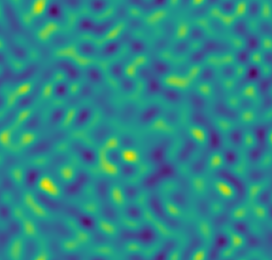
\includegraphics[interpolate=true,width=2.520000in,height=2.380000in]{burgers_solution_0.01-img0.png}}%
\end{pgfscope}%
\begin{pgfscope}%
\pgfsetbuttcap%
\pgfsetroundjoin%
\definecolor{currentfill}{rgb}{0.000000,0.000000,0.000000}%
\pgfsetfillcolor{currentfill}%
\pgfsetlinewidth{0.803000pt}%
\definecolor{currentstroke}{rgb}{0.000000,0.000000,0.000000}%
\pgfsetstrokecolor{currentstroke}%
\pgfsetdash{}{0pt}%
\pgfsys@defobject{currentmarker}{\pgfqpoint{0.000000in}{-0.048611in}}{\pgfqpoint{0.000000in}{0.000000in}}{%
\pgfpathmoveto{\pgfqpoint{0.000000in}{0.000000in}}%
\pgfpathlineto{\pgfqpoint{0.000000in}{-0.048611in}}%
\pgfusepath{stroke,fill}%
}%
\begin{pgfscope}%
\pgfsys@transformshift{0.567820in}{0.517039in}%
\pgfsys@useobject{currentmarker}{}%
\end{pgfscope}%
\end{pgfscope}%
\begin{pgfscope}%
\definecolor{textcolor}{rgb}{0.000000,0.000000,0.000000}%
\pgfsetstrokecolor{textcolor}%
\pgfsetfillcolor{textcolor}%
\pgftext[x=0.567820in,y=0.419816in,,top]{\color{textcolor}\rmfamily\fontsize{12.000000}{14.400000}\selectfont 0.0}%
\end{pgfscope}%
\begin{pgfscope}%
\pgfsetbuttcap%
\pgfsetroundjoin%
\definecolor{currentfill}{rgb}{0.000000,0.000000,0.000000}%
\pgfsetfillcolor{currentfill}%
\pgfsetlinewidth{0.803000pt}%
\definecolor{currentstroke}{rgb}{0.000000,0.000000,0.000000}%
\pgfsetstrokecolor{currentstroke}%
\pgfsetdash{}{0pt}%
\pgfsys@defobject{currentmarker}{\pgfqpoint{0.000000in}{-0.048611in}}{\pgfqpoint{0.000000in}{0.000000in}}{%
\pgfpathmoveto{\pgfqpoint{0.000000in}{0.000000in}}%
\pgfpathlineto{\pgfqpoint{0.000000in}{-0.048611in}}%
\pgfusepath{stroke,fill}%
}%
\begin{pgfscope}%
\pgfsys@transformshift{1.196524in}{0.517039in}%
\pgfsys@useobject{currentmarker}{}%
\end{pgfscope}%
\end{pgfscope}%
\begin{pgfscope}%
\definecolor{textcolor}{rgb}{0.000000,0.000000,0.000000}%
\pgfsetstrokecolor{textcolor}%
\pgfsetfillcolor{textcolor}%
\pgftext[x=1.196524in,y=0.419816in,,top]{\color{textcolor}\rmfamily\fontsize{12.000000}{14.400000}\selectfont 0.5}%
\end{pgfscope}%
\begin{pgfscope}%
\pgfsetbuttcap%
\pgfsetroundjoin%
\definecolor{currentfill}{rgb}{0.000000,0.000000,0.000000}%
\pgfsetfillcolor{currentfill}%
\pgfsetlinewidth{0.803000pt}%
\definecolor{currentstroke}{rgb}{0.000000,0.000000,0.000000}%
\pgfsetstrokecolor{currentstroke}%
\pgfsetdash{}{0pt}%
\pgfsys@defobject{currentmarker}{\pgfqpoint{0.000000in}{-0.048611in}}{\pgfqpoint{0.000000in}{0.000000in}}{%
\pgfpathmoveto{\pgfqpoint{0.000000in}{0.000000in}}%
\pgfpathlineto{\pgfqpoint{0.000000in}{-0.048611in}}%
\pgfusepath{stroke,fill}%
}%
\begin{pgfscope}%
\pgfsys@transformshift{1.825229in}{0.517039in}%
\pgfsys@useobject{currentmarker}{}%
\end{pgfscope}%
\end{pgfscope}%
\begin{pgfscope}%
\definecolor{textcolor}{rgb}{0.000000,0.000000,0.000000}%
\pgfsetstrokecolor{textcolor}%
\pgfsetfillcolor{textcolor}%
\pgftext[x=1.825229in,y=0.419816in,,top]{\color{textcolor}\rmfamily\fontsize{12.000000}{14.400000}\selectfont 1.0}%
\end{pgfscope}%
\begin{pgfscope}%
\pgfsetbuttcap%
\pgfsetroundjoin%
\definecolor{currentfill}{rgb}{0.000000,0.000000,0.000000}%
\pgfsetfillcolor{currentfill}%
\pgfsetlinewidth{0.803000pt}%
\definecolor{currentstroke}{rgb}{0.000000,0.000000,0.000000}%
\pgfsetstrokecolor{currentstroke}%
\pgfsetdash{}{0pt}%
\pgfsys@defobject{currentmarker}{\pgfqpoint{0.000000in}{-0.048611in}}{\pgfqpoint{0.000000in}{0.000000in}}{%
\pgfpathmoveto{\pgfqpoint{0.000000in}{0.000000in}}%
\pgfpathlineto{\pgfqpoint{0.000000in}{-0.048611in}}%
\pgfusepath{stroke,fill}%
}%
\begin{pgfscope}%
\pgfsys@transformshift{2.453933in}{0.517039in}%
\pgfsys@useobject{currentmarker}{}%
\end{pgfscope}%
\end{pgfscope}%
\begin{pgfscope}%
\definecolor{textcolor}{rgb}{0.000000,0.000000,0.000000}%
\pgfsetstrokecolor{textcolor}%
\pgfsetfillcolor{textcolor}%
\pgftext[x=2.453933in,y=0.419816in,,top]{\color{textcolor}\rmfamily\fontsize{12.000000}{14.400000}\selectfont 1.5}%
\end{pgfscope}%
\begin{pgfscope}%
\pgfsetbuttcap%
\pgfsetroundjoin%
\definecolor{currentfill}{rgb}{0.000000,0.000000,0.000000}%
\pgfsetfillcolor{currentfill}%
\pgfsetlinewidth{0.803000pt}%
\definecolor{currentstroke}{rgb}{0.000000,0.000000,0.000000}%
\pgfsetstrokecolor{currentstroke}%
\pgfsetdash{}{0pt}%
\pgfsys@defobject{currentmarker}{\pgfqpoint{0.000000in}{-0.048611in}}{\pgfqpoint{0.000000in}{0.000000in}}{%
\pgfpathmoveto{\pgfqpoint{0.000000in}{0.000000in}}%
\pgfpathlineto{\pgfqpoint{0.000000in}{-0.048611in}}%
\pgfusepath{stroke,fill}%
}%
\begin{pgfscope}%
\pgfsys@transformshift{3.082637in}{0.517039in}%
\pgfsys@useobject{currentmarker}{}%
\end{pgfscope}%
\end{pgfscope}%
\begin{pgfscope}%
\definecolor{textcolor}{rgb}{0.000000,0.000000,0.000000}%
\pgfsetstrokecolor{textcolor}%
\pgfsetfillcolor{textcolor}%
\pgftext[x=3.082637in,y=0.419816in,,top]{\color{textcolor}\rmfamily\fontsize{12.000000}{14.400000}\selectfont 2.0}%
\end{pgfscope}%
\begin{pgfscope}%
\definecolor{textcolor}{rgb}{0.000000,0.000000,0.000000}%
\pgfsetstrokecolor{textcolor}%
\pgfsetfillcolor{textcolor}%
\pgftext[x=1.825229in,y=0.202965in,,top]{\color{textcolor}\rmfamily\fontsize{12.000000}{14.400000}\selectfont Space}%
\end{pgfscope}%
\begin{pgfscope}%
\pgfsetbuttcap%
\pgfsetroundjoin%
\definecolor{currentfill}{rgb}{0.000000,0.000000,0.000000}%
\pgfsetfillcolor{currentfill}%
\pgfsetlinewidth{0.803000pt}%
\definecolor{currentstroke}{rgb}{0.000000,0.000000,0.000000}%
\pgfsetstrokecolor{currentstroke}%
\pgfsetdash{}{0pt}%
\pgfsys@defobject{currentmarker}{\pgfqpoint{-0.048611in}{0.000000in}}{\pgfqpoint{-0.000000in}{0.000000in}}{%
\pgfpathmoveto{\pgfqpoint{-0.000000in}{0.000000in}}%
\pgfpathlineto{\pgfqpoint{-0.048611in}{0.000000in}}%
\pgfusepath{stroke,fill}%
}%
\begin{pgfscope}%
\pgfsys@transformshift{0.567820in}{0.517039in}%
\pgfsys@useobject{currentmarker}{}%
\end{pgfscope}%
\end{pgfscope}%
\begin{pgfscope}%
\definecolor{textcolor}{rgb}{0.000000,0.000000,0.000000}%
\pgfsetstrokecolor{textcolor}%
\pgfsetfillcolor{textcolor}%
\pgftext[x=0.364559in, y=0.453725in, left, base]{\color{textcolor}\rmfamily\fontsize{12.000000}{14.400000}\selectfont 0}%
\end{pgfscope}%
\begin{pgfscope}%
\pgfsetbuttcap%
\pgfsetroundjoin%
\definecolor{currentfill}{rgb}{0.000000,0.000000,0.000000}%
\pgfsetfillcolor{currentfill}%
\pgfsetlinewidth{0.803000pt}%
\definecolor{currentstroke}{rgb}{0.000000,0.000000,0.000000}%
\pgfsetstrokecolor{currentstroke}%
\pgfsetdash{}{0pt}%
\pgfsys@defobject{currentmarker}{\pgfqpoint{-0.048611in}{0.000000in}}{\pgfqpoint{-0.000000in}{0.000000in}}{%
\pgfpathmoveto{\pgfqpoint{-0.000000in}{0.000000in}}%
\pgfpathlineto{\pgfqpoint{-0.048611in}{0.000000in}}%
\pgfusepath{stroke,fill}%
}%
\begin{pgfscope}%
\pgfsys@transformshift{0.567820in}{0.992634in}%
\pgfsys@useobject{currentmarker}{}%
\end{pgfscope}%
\end{pgfscope}%
\begin{pgfscope}%
\definecolor{textcolor}{rgb}{0.000000,0.000000,0.000000}%
\pgfsetstrokecolor{textcolor}%
\pgfsetfillcolor{textcolor}%
\pgftext[x=0.364559in, y=0.929320in, left, base]{\color{textcolor}\rmfamily\fontsize{12.000000}{14.400000}\selectfont 2}%
\end{pgfscope}%
\begin{pgfscope}%
\pgfsetbuttcap%
\pgfsetroundjoin%
\definecolor{currentfill}{rgb}{0.000000,0.000000,0.000000}%
\pgfsetfillcolor{currentfill}%
\pgfsetlinewidth{0.803000pt}%
\definecolor{currentstroke}{rgb}{0.000000,0.000000,0.000000}%
\pgfsetstrokecolor{currentstroke}%
\pgfsetdash{}{0pt}%
\pgfsys@defobject{currentmarker}{\pgfqpoint{-0.048611in}{0.000000in}}{\pgfqpoint{-0.000000in}{0.000000in}}{%
\pgfpathmoveto{\pgfqpoint{-0.000000in}{0.000000in}}%
\pgfpathlineto{\pgfqpoint{-0.048611in}{0.000000in}}%
\pgfusepath{stroke,fill}%
}%
\begin{pgfscope}%
\pgfsys@transformshift{0.567820in}{1.468230in}%
\pgfsys@useobject{currentmarker}{}%
\end{pgfscope}%
\end{pgfscope}%
\begin{pgfscope}%
\definecolor{textcolor}{rgb}{0.000000,0.000000,0.000000}%
\pgfsetstrokecolor{textcolor}%
\pgfsetfillcolor{textcolor}%
\pgftext[x=0.364559in, y=1.404916in, left, base]{\color{textcolor}\rmfamily\fontsize{12.000000}{14.400000}\selectfont 4}%
\end{pgfscope}%
\begin{pgfscope}%
\pgfsetbuttcap%
\pgfsetroundjoin%
\definecolor{currentfill}{rgb}{0.000000,0.000000,0.000000}%
\pgfsetfillcolor{currentfill}%
\pgfsetlinewidth{0.803000pt}%
\definecolor{currentstroke}{rgb}{0.000000,0.000000,0.000000}%
\pgfsetstrokecolor{currentstroke}%
\pgfsetdash{}{0pt}%
\pgfsys@defobject{currentmarker}{\pgfqpoint{-0.048611in}{0.000000in}}{\pgfqpoint{-0.000000in}{0.000000in}}{%
\pgfpathmoveto{\pgfqpoint{-0.000000in}{0.000000in}}%
\pgfpathlineto{\pgfqpoint{-0.048611in}{0.000000in}}%
\pgfusepath{stroke,fill}%
}%
\begin{pgfscope}%
\pgfsys@transformshift{0.567820in}{1.943825in}%
\pgfsys@useobject{currentmarker}{}%
\end{pgfscope}%
\end{pgfscope}%
\begin{pgfscope}%
\definecolor{textcolor}{rgb}{0.000000,0.000000,0.000000}%
\pgfsetstrokecolor{textcolor}%
\pgfsetfillcolor{textcolor}%
\pgftext[x=0.364559in, y=1.880511in, left, base]{\color{textcolor}\rmfamily\fontsize{12.000000}{14.400000}\selectfont 6}%
\end{pgfscope}%
\begin{pgfscope}%
\pgfsetbuttcap%
\pgfsetroundjoin%
\definecolor{currentfill}{rgb}{0.000000,0.000000,0.000000}%
\pgfsetfillcolor{currentfill}%
\pgfsetlinewidth{0.803000pt}%
\definecolor{currentstroke}{rgb}{0.000000,0.000000,0.000000}%
\pgfsetstrokecolor{currentstroke}%
\pgfsetdash{}{0pt}%
\pgfsys@defobject{currentmarker}{\pgfqpoint{-0.048611in}{0.000000in}}{\pgfqpoint{-0.000000in}{0.000000in}}{%
\pgfpathmoveto{\pgfqpoint{-0.000000in}{0.000000in}}%
\pgfpathlineto{\pgfqpoint{-0.048611in}{0.000000in}}%
\pgfusepath{stroke,fill}%
}%
\begin{pgfscope}%
\pgfsys@transformshift{0.567820in}{2.419421in}%
\pgfsys@useobject{currentmarker}{}%
\end{pgfscope}%
\end{pgfscope}%
\begin{pgfscope}%
\definecolor{textcolor}{rgb}{0.000000,0.000000,0.000000}%
\pgfsetstrokecolor{textcolor}%
\pgfsetfillcolor{textcolor}%
\pgftext[x=0.364559in, y=2.356107in, left, base]{\color{textcolor}\rmfamily\fontsize{12.000000}{14.400000}\selectfont 8}%
\end{pgfscope}%
\begin{pgfscope}%
\pgfsetbuttcap%
\pgfsetroundjoin%
\definecolor{currentfill}{rgb}{0.000000,0.000000,0.000000}%
\pgfsetfillcolor{currentfill}%
\pgfsetlinewidth{0.803000pt}%
\definecolor{currentstroke}{rgb}{0.000000,0.000000,0.000000}%
\pgfsetstrokecolor{currentstroke}%
\pgfsetdash{}{0pt}%
\pgfsys@defobject{currentmarker}{\pgfqpoint{-0.048611in}{0.000000in}}{\pgfqpoint{-0.000000in}{0.000000in}}{%
\pgfpathmoveto{\pgfqpoint{-0.000000in}{0.000000in}}%
\pgfpathlineto{\pgfqpoint{-0.048611in}{0.000000in}}%
\pgfusepath{stroke,fill}%
}%
\begin{pgfscope}%
\pgfsys@transformshift{0.567820in}{2.895016in}%
\pgfsys@useobject{currentmarker}{}%
\end{pgfscope}%
\end{pgfscope}%
\begin{pgfscope}%
\definecolor{textcolor}{rgb}{0.000000,0.000000,0.000000}%
\pgfsetstrokecolor{textcolor}%
\pgfsetfillcolor{textcolor}%
\pgftext[x=0.258521in, y=2.831702in, left, base]{\color{textcolor}\rmfamily\fontsize{12.000000}{14.400000}\selectfont 10}%
\end{pgfscope}%
\begin{pgfscope}%
\definecolor{textcolor}{rgb}{0.000000,0.000000,0.000000}%
\pgfsetstrokecolor{textcolor}%
\pgfsetfillcolor{textcolor}%
\pgftext[x=0.202965in,y=1.706027in,,bottom,rotate=90.000000]{\color{textcolor}\rmfamily\fontsize{12.000000}{14.400000}\selectfont Time}%
\end{pgfscope}%
\begin{pgfscope}%
\pgfsetrectcap%
\pgfsetmiterjoin%
\pgfsetlinewidth{0.803000pt}%
\definecolor{currentstroke}{rgb}{0.000000,0.000000,0.000000}%
\pgfsetstrokecolor{currentstroke}%
\pgfsetdash{}{0pt}%
\pgfpathmoveto{\pgfqpoint{0.567820in}{0.517039in}}%
\pgfpathlineto{\pgfqpoint{0.567820in}{2.895016in}}%
\pgfusepath{stroke}%
\end{pgfscope}%
\begin{pgfscope}%
\pgfsetrectcap%
\pgfsetmiterjoin%
\pgfsetlinewidth{0.803000pt}%
\definecolor{currentstroke}{rgb}{0.000000,0.000000,0.000000}%
\pgfsetstrokecolor{currentstroke}%
\pgfsetdash{}{0pt}%
\pgfpathmoveto{\pgfqpoint{3.082637in}{0.517039in}}%
\pgfpathlineto{\pgfqpoint{3.082637in}{2.895016in}}%
\pgfusepath{stroke}%
\end{pgfscope}%
\begin{pgfscope}%
\pgfsetrectcap%
\pgfsetmiterjoin%
\pgfsetlinewidth{0.803000pt}%
\definecolor{currentstroke}{rgb}{0.000000,0.000000,0.000000}%
\pgfsetstrokecolor{currentstroke}%
\pgfsetdash{}{0pt}%
\pgfpathmoveto{\pgfqpoint{0.567820in}{0.517039in}}%
\pgfpathlineto{\pgfqpoint{3.082637in}{0.517039in}}%
\pgfusepath{stroke}%
\end{pgfscope}%
\begin{pgfscope}%
\pgfsetrectcap%
\pgfsetmiterjoin%
\pgfsetlinewidth{0.803000pt}%
\definecolor{currentstroke}{rgb}{0.000000,0.000000,0.000000}%
\pgfsetstrokecolor{currentstroke}%
\pgfsetdash{}{0pt}%
\pgfpathmoveto{\pgfqpoint{0.567820in}{2.895016in}}%
\pgfpathlineto{\pgfqpoint{3.082637in}{2.895016in}}%
\pgfusepath{stroke}%
\end{pgfscope}%
\begin{pgfscope}%
\pgfsetbuttcap%
\pgfsetmiterjoin%
\pgfsetlinewidth{0.000000pt}%
\definecolor{currentstroke}{rgb}{0.000000,0.000000,0.000000}%
\pgfsetstrokecolor{currentstroke}%
\pgfsetstrokeopacity{0.000000}%
\pgfsetdash{}{0pt}%
\pgfpathmoveto{\pgfqpoint{3.340906in}{0.517039in}}%
\pgfpathlineto{\pgfqpoint{3.459805in}{0.517039in}}%
\pgfpathlineto{\pgfqpoint{3.459805in}{2.895016in}}%
\pgfpathlineto{\pgfqpoint{3.340906in}{2.895016in}}%
\pgfpathlineto{\pgfqpoint{3.340906in}{0.517039in}}%
\pgfpathclose%
\pgfusepath{}%
\end{pgfscope}%
\begin{pgfscope}%
\pgfsys@transformshift{3.340000in}{0.520000in}%
\pgftext[left,bottom]{
\includegraphics[interpolate=true,width=0.120000in,height=2.380000in]{burgers_solution_0.01-img1.png}}%
\end{pgfscope}%
\begin{pgfscope}%
\pgfsetbuttcap%
\pgfsetroundjoin%
\definecolor{currentfill}{rgb}{0.000000,0.000000,0.000000}%
\pgfsetfillcolor{currentfill}%
\pgfsetlinewidth{0.803000pt}%
\definecolor{currentstroke}{rgb}{0.000000,0.000000,0.000000}%
\pgfsetstrokecolor{currentstroke}%
\pgfsetdash{}{0pt}%
\pgfsys@defobject{currentmarker}{\pgfqpoint{0.000000in}{0.000000in}}{\pgfqpoint{0.048611in}{0.000000in}}{%
\pgfpathmoveto{\pgfqpoint{0.000000in}{0.000000in}}%
\pgfpathlineto{\pgfqpoint{0.048611in}{0.000000in}}%
\pgfusepath{stroke,fill}%
}%
\begin{pgfscope}%
\pgfsys@transformshift{3.459805in}{0.555741in}%
\pgfsys@useobject{currentmarker}{}%
\end{pgfscope}%
\end{pgfscope}%
\begin{pgfscope}%
\definecolor{textcolor}{rgb}{0.000000,0.000000,0.000000}%
\pgfsetstrokecolor{textcolor}%
\pgfsetfillcolor{textcolor}%
\pgftext[x=3.557027in, y=0.492427in, left, base]{\color{textcolor}\rmfamily\fontsize{12.000000}{14.400000}\selectfont \ensuremath{-}0.6}%
\end{pgfscope}%
\begin{pgfscope}%
\pgfsetbuttcap%
\pgfsetroundjoin%
\definecolor{currentfill}{rgb}{0.000000,0.000000,0.000000}%
\pgfsetfillcolor{currentfill}%
\pgfsetlinewidth{0.803000pt}%
\definecolor{currentstroke}{rgb}{0.000000,0.000000,0.000000}%
\pgfsetstrokecolor{currentstroke}%
\pgfsetdash{}{0pt}%
\pgfsys@defobject{currentmarker}{\pgfqpoint{0.000000in}{0.000000in}}{\pgfqpoint{0.048611in}{0.000000in}}{%
\pgfpathmoveto{\pgfqpoint{0.000000in}{0.000000in}}%
\pgfpathlineto{\pgfqpoint{0.048611in}{0.000000in}}%
\pgfusepath{stroke,fill}%
}%
\begin{pgfscope}%
\pgfsys@transformshift{3.459805in}{0.932008in}%
\pgfsys@useobject{currentmarker}{}%
\end{pgfscope}%
\end{pgfscope}%
\begin{pgfscope}%
\definecolor{textcolor}{rgb}{0.000000,0.000000,0.000000}%
\pgfsetstrokecolor{textcolor}%
\pgfsetfillcolor{textcolor}%
\pgftext[x=3.557027in, y=0.868694in, left, base]{\color{textcolor}\rmfamily\fontsize{12.000000}{14.400000}\selectfont \ensuremath{-}0.4}%
\end{pgfscope}%
\begin{pgfscope}%
\pgfsetbuttcap%
\pgfsetroundjoin%
\definecolor{currentfill}{rgb}{0.000000,0.000000,0.000000}%
\pgfsetfillcolor{currentfill}%
\pgfsetlinewidth{0.803000pt}%
\definecolor{currentstroke}{rgb}{0.000000,0.000000,0.000000}%
\pgfsetstrokecolor{currentstroke}%
\pgfsetdash{}{0pt}%
\pgfsys@defobject{currentmarker}{\pgfqpoint{0.000000in}{0.000000in}}{\pgfqpoint{0.048611in}{0.000000in}}{%
\pgfpathmoveto{\pgfqpoint{0.000000in}{0.000000in}}%
\pgfpathlineto{\pgfqpoint{0.048611in}{0.000000in}}%
\pgfusepath{stroke,fill}%
}%
\begin{pgfscope}%
\pgfsys@transformshift{3.459805in}{1.308274in}%
\pgfsys@useobject{currentmarker}{}%
\end{pgfscope}%
\end{pgfscope}%
\begin{pgfscope}%
\definecolor{textcolor}{rgb}{0.000000,0.000000,0.000000}%
\pgfsetstrokecolor{textcolor}%
\pgfsetfillcolor{textcolor}%
\pgftext[x=3.557027in, y=1.244961in, left, base]{\color{textcolor}\rmfamily\fontsize{12.000000}{14.400000}\selectfont \ensuremath{-}0.2}%
\end{pgfscope}%
\begin{pgfscope}%
\pgfsetbuttcap%
\pgfsetroundjoin%
\definecolor{currentfill}{rgb}{0.000000,0.000000,0.000000}%
\pgfsetfillcolor{currentfill}%
\pgfsetlinewidth{0.803000pt}%
\definecolor{currentstroke}{rgb}{0.000000,0.000000,0.000000}%
\pgfsetstrokecolor{currentstroke}%
\pgfsetdash{}{0pt}%
\pgfsys@defobject{currentmarker}{\pgfqpoint{0.000000in}{0.000000in}}{\pgfqpoint{0.048611in}{0.000000in}}{%
\pgfpathmoveto{\pgfqpoint{0.000000in}{0.000000in}}%
\pgfpathlineto{\pgfqpoint{0.048611in}{0.000000in}}%
\pgfusepath{stroke,fill}%
}%
\begin{pgfscope}%
\pgfsys@transformshift{3.459805in}{1.684541in}%
\pgfsys@useobject{currentmarker}{}%
\end{pgfscope}%
\end{pgfscope}%
\begin{pgfscope}%
\definecolor{textcolor}{rgb}{0.000000,0.000000,0.000000}%
\pgfsetstrokecolor{textcolor}%
\pgfsetfillcolor{textcolor}%
\pgftext[x=3.557027in, y=1.621228in, left, base]{\color{textcolor}\rmfamily\fontsize{12.000000}{14.400000}\selectfont 0.0}%
\end{pgfscope}%
\begin{pgfscope}%
\pgfsetbuttcap%
\pgfsetroundjoin%
\definecolor{currentfill}{rgb}{0.000000,0.000000,0.000000}%
\pgfsetfillcolor{currentfill}%
\pgfsetlinewidth{0.803000pt}%
\definecolor{currentstroke}{rgb}{0.000000,0.000000,0.000000}%
\pgfsetstrokecolor{currentstroke}%
\pgfsetdash{}{0pt}%
\pgfsys@defobject{currentmarker}{\pgfqpoint{0.000000in}{0.000000in}}{\pgfqpoint{0.048611in}{0.000000in}}{%
\pgfpathmoveto{\pgfqpoint{0.000000in}{0.000000in}}%
\pgfpathlineto{\pgfqpoint{0.048611in}{0.000000in}}%
\pgfusepath{stroke,fill}%
}%
\begin{pgfscope}%
\pgfsys@transformshift{3.459805in}{2.060808in}%
\pgfsys@useobject{currentmarker}{}%
\end{pgfscope}%
\end{pgfscope}%
\begin{pgfscope}%
\definecolor{textcolor}{rgb}{0.000000,0.000000,0.000000}%
\pgfsetstrokecolor{textcolor}%
\pgfsetfillcolor{textcolor}%
\pgftext[x=3.557027in, y=1.997494in, left, base]{\color{textcolor}\rmfamily\fontsize{12.000000}{14.400000}\selectfont 0.2}%
\end{pgfscope}%
\begin{pgfscope}%
\pgfsetbuttcap%
\pgfsetroundjoin%
\definecolor{currentfill}{rgb}{0.000000,0.000000,0.000000}%
\pgfsetfillcolor{currentfill}%
\pgfsetlinewidth{0.803000pt}%
\definecolor{currentstroke}{rgb}{0.000000,0.000000,0.000000}%
\pgfsetstrokecolor{currentstroke}%
\pgfsetdash{}{0pt}%
\pgfsys@defobject{currentmarker}{\pgfqpoint{0.000000in}{0.000000in}}{\pgfqpoint{0.048611in}{0.000000in}}{%
\pgfpathmoveto{\pgfqpoint{0.000000in}{0.000000in}}%
\pgfpathlineto{\pgfqpoint{0.048611in}{0.000000in}}%
\pgfusepath{stroke,fill}%
}%
\begin{pgfscope}%
\pgfsys@transformshift{3.459805in}{2.437075in}%
\pgfsys@useobject{currentmarker}{}%
\end{pgfscope}%
\end{pgfscope}%
\begin{pgfscope}%
\definecolor{textcolor}{rgb}{0.000000,0.000000,0.000000}%
\pgfsetstrokecolor{textcolor}%
\pgfsetfillcolor{textcolor}%
\pgftext[x=3.557027in, y=2.373761in, left, base]{\color{textcolor}\rmfamily\fontsize{12.000000}{14.400000}\selectfont 0.4}%
\end{pgfscope}%
\begin{pgfscope}%
\pgfsetbuttcap%
\pgfsetroundjoin%
\definecolor{currentfill}{rgb}{0.000000,0.000000,0.000000}%
\pgfsetfillcolor{currentfill}%
\pgfsetlinewidth{0.803000pt}%
\definecolor{currentstroke}{rgb}{0.000000,0.000000,0.000000}%
\pgfsetstrokecolor{currentstroke}%
\pgfsetdash{}{0pt}%
\pgfsys@defobject{currentmarker}{\pgfqpoint{0.000000in}{0.000000in}}{\pgfqpoint{0.048611in}{0.000000in}}{%
\pgfpathmoveto{\pgfqpoint{0.000000in}{0.000000in}}%
\pgfpathlineto{\pgfqpoint{0.048611in}{0.000000in}}%
\pgfusepath{stroke,fill}%
}%
\begin{pgfscope}%
\pgfsys@transformshift{3.459805in}{2.813342in}%
\pgfsys@useobject{currentmarker}{}%
\end{pgfscope}%
\end{pgfscope}%
\begin{pgfscope}%
\definecolor{textcolor}{rgb}{0.000000,0.000000,0.000000}%
\pgfsetstrokecolor{textcolor}%
\pgfsetfillcolor{textcolor}%
\pgftext[x=3.557027in, y=2.750028in, left, base]{\color{textcolor}\rmfamily\fontsize{12.000000}{14.400000}\selectfont 0.6}%
\end{pgfscope}%
\begin{pgfscope}%
\pgfsetrectcap%
\pgfsetmiterjoin%
\pgfsetlinewidth{0.803000pt}%
\definecolor{currentstroke}{rgb}{0.000000,0.000000,0.000000}%
\pgfsetstrokecolor{currentstroke}%
\pgfsetdash{}{0pt}%
\pgfpathmoveto{\pgfqpoint{3.340906in}{0.517039in}}%
\pgfpathlineto{\pgfqpoint{3.400355in}{0.517039in}}%
\pgfpathlineto{\pgfqpoint{3.459805in}{0.517039in}}%
\pgfpathlineto{\pgfqpoint{3.459805in}{2.895016in}}%
\pgfpathlineto{\pgfqpoint{3.400355in}{2.895016in}}%
\pgfpathlineto{\pgfqpoint{3.340906in}{2.895016in}}%
\pgfpathlineto{\pgfqpoint{3.340906in}{0.517039in}}%
\pgfpathclose%
\pgfusepath{stroke}%
\end{pgfscope}%
\end{pgfpicture}%
\makeatother%
\endgroup%

    \end{adjustbox}
    \caption{Solution function for \(\nu=0.01\).}\label{fig:burgers_solution_0.01}
  \end{subfigure}
  \begin{subfigure}{0.49\linewidth}
    \begin{adjustbox}{width=\linewidth}
      \begingroup%
\makeatletter%
\begin{pgfpicture}%
\pgfpathrectangle{\pgfpointorigin}{\pgfqpoint{4.000000in}{3.000000in}}%
\pgfusepath{use as bounding box, clip}%
\begin{pgfscope}%
\pgfsetbuttcap%
\pgfsetmiterjoin%
\pgfsetlinewidth{0.000000pt}%
\definecolor{currentstroke}{rgb}{0.000000,0.000000,0.000000}%
\pgfsetstrokecolor{currentstroke}%
\pgfsetstrokeopacity{0.000000}%
\pgfsetdash{}{0pt}%
\pgfpathmoveto{\pgfqpoint{0.000000in}{0.000000in}}%
\pgfpathlineto{\pgfqpoint{4.000000in}{0.000000in}}%
\pgfpathlineto{\pgfqpoint{4.000000in}{3.000000in}}%
\pgfpathlineto{\pgfqpoint{0.000000in}{3.000000in}}%
\pgfpathlineto{\pgfqpoint{0.000000in}{0.000000in}}%
\pgfpathclose%
\pgfusepath{}%
\end{pgfscope}%
\begin{pgfscope}%
\pgfsetbuttcap%
\pgfsetmiterjoin%
\pgfsetlinewidth{0.000000pt}%
\definecolor{currentstroke}{rgb}{0.000000,0.000000,0.000000}%
\pgfsetstrokecolor{currentstroke}%
\pgfsetstrokeopacity{0.000000}%
\pgfsetdash{}{0pt}%
\pgfpathmoveto{\pgfqpoint{0.567820in}{0.517039in}}%
\pgfpathlineto{\pgfqpoint{3.082637in}{0.517039in}}%
\pgfpathlineto{\pgfqpoint{3.082637in}{2.895016in}}%
\pgfpathlineto{\pgfqpoint{0.567820in}{2.895016in}}%
\pgfpathlineto{\pgfqpoint{0.567820in}{0.517039in}}%
\pgfpathclose%
\pgfusepath{}%
\end{pgfscope}%
\begin{pgfscope}%
\pgfpathrectangle{\pgfqpoint{0.567820in}{0.517039in}}{\pgfqpoint{2.514817in}{2.377978in}}%
\pgfusepath{clip}%
\pgfsys@transformshift{0.567820in}{0.517039in}%
\pgftext[left,bottom]{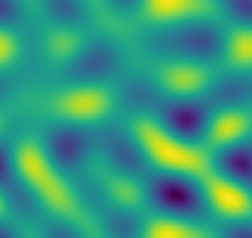
\includegraphics[interpolate=true,width=2.520000in,height=2.380000in]{burgers_forcing_0.01-img0.png}}%
\end{pgfscope}%
\begin{pgfscope}%
\pgfsetbuttcap%
\pgfsetroundjoin%
\definecolor{currentfill}{rgb}{0.000000,0.000000,0.000000}%
\pgfsetfillcolor{currentfill}%
\pgfsetlinewidth{0.803000pt}%
\definecolor{currentstroke}{rgb}{0.000000,0.000000,0.000000}%
\pgfsetstrokecolor{currentstroke}%
\pgfsetdash{}{0pt}%
\pgfsys@defobject{currentmarker}{\pgfqpoint{0.000000in}{-0.048611in}}{\pgfqpoint{0.000000in}{0.000000in}}{%
\pgfpathmoveto{\pgfqpoint{0.000000in}{0.000000in}}%
\pgfpathlineto{\pgfqpoint{0.000000in}{-0.048611in}}%
\pgfusepath{stroke,fill}%
}%
\begin{pgfscope}%
\pgfsys@transformshift{0.567820in}{0.517039in}%
\pgfsys@useobject{currentmarker}{}%
\end{pgfscope}%
\end{pgfscope}%
\begin{pgfscope}%
\definecolor{textcolor}{rgb}{0.000000,0.000000,0.000000}%
\pgfsetstrokecolor{textcolor}%
\pgfsetfillcolor{textcolor}%
\pgftext[x=0.567820in,y=0.419816in,,top]{\color{textcolor}\rmfamily\fontsize{12.000000}{14.400000}\selectfont 0.0}%
\end{pgfscope}%
\begin{pgfscope}%
\pgfsetbuttcap%
\pgfsetroundjoin%
\definecolor{currentfill}{rgb}{0.000000,0.000000,0.000000}%
\pgfsetfillcolor{currentfill}%
\pgfsetlinewidth{0.803000pt}%
\definecolor{currentstroke}{rgb}{0.000000,0.000000,0.000000}%
\pgfsetstrokecolor{currentstroke}%
\pgfsetdash{}{0pt}%
\pgfsys@defobject{currentmarker}{\pgfqpoint{0.000000in}{-0.048611in}}{\pgfqpoint{0.000000in}{0.000000in}}{%
\pgfpathmoveto{\pgfqpoint{0.000000in}{0.000000in}}%
\pgfpathlineto{\pgfqpoint{0.000000in}{-0.048611in}}%
\pgfusepath{stroke,fill}%
}%
\begin{pgfscope}%
\pgfsys@transformshift{1.196524in}{0.517039in}%
\pgfsys@useobject{currentmarker}{}%
\end{pgfscope}%
\end{pgfscope}%
\begin{pgfscope}%
\definecolor{textcolor}{rgb}{0.000000,0.000000,0.000000}%
\pgfsetstrokecolor{textcolor}%
\pgfsetfillcolor{textcolor}%
\pgftext[x=1.196524in,y=0.419816in,,top]{\color{textcolor}\rmfamily\fontsize{12.000000}{14.400000}\selectfont 0.5}%
\end{pgfscope}%
\begin{pgfscope}%
\pgfsetbuttcap%
\pgfsetroundjoin%
\definecolor{currentfill}{rgb}{0.000000,0.000000,0.000000}%
\pgfsetfillcolor{currentfill}%
\pgfsetlinewidth{0.803000pt}%
\definecolor{currentstroke}{rgb}{0.000000,0.000000,0.000000}%
\pgfsetstrokecolor{currentstroke}%
\pgfsetdash{}{0pt}%
\pgfsys@defobject{currentmarker}{\pgfqpoint{0.000000in}{-0.048611in}}{\pgfqpoint{0.000000in}{0.000000in}}{%
\pgfpathmoveto{\pgfqpoint{0.000000in}{0.000000in}}%
\pgfpathlineto{\pgfqpoint{0.000000in}{-0.048611in}}%
\pgfusepath{stroke,fill}%
}%
\begin{pgfscope}%
\pgfsys@transformshift{1.825229in}{0.517039in}%
\pgfsys@useobject{currentmarker}{}%
\end{pgfscope}%
\end{pgfscope}%
\begin{pgfscope}%
\definecolor{textcolor}{rgb}{0.000000,0.000000,0.000000}%
\pgfsetstrokecolor{textcolor}%
\pgfsetfillcolor{textcolor}%
\pgftext[x=1.825229in,y=0.419816in,,top]{\color{textcolor}\rmfamily\fontsize{12.000000}{14.400000}\selectfont 1.0}%
\end{pgfscope}%
\begin{pgfscope}%
\pgfsetbuttcap%
\pgfsetroundjoin%
\definecolor{currentfill}{rgb}{0.000000,0.000000,0.000000}%
\pgfsetfillcolor{currentfill}%
\pgfsetlinewidth{0.803000pt}%
\definecolor{currentstroke}{rgb}{0.000000,0.000000,0.000000}%
\pgfsetstrokecolor{currentstroke}%
\pgfsetdash{}{0pt}%
\pgfsys@defobject{currentmarker}{\pgfqpoint{0.000000in}{-0.048611in}}{\pgfqpoint{0.000000in}{0.000000in}}{%
\pgfpathmoveto{\pgfqpoint{0.000000in}{0.000000in}}%
\pgfpathlineto{\pgfqpoint{0.000000in}{-0.048611in}}%
\pgfusepath{stroke,fill}%
}%
\begin{pgfscope}%
\pgfsys@transformshift{2.453933in}{0.517039in}%
\pgfsys@useobject{currentmarker}{}%
\end{pgfscope}%
\end{pgfscope}%
\begin{pgfscope}%
\definecolor{textcolor}{rgb}{0.000000,0.000000,0.000000}%
\pgfsetstrokecolor{textcolor}%
\pgfsetfillcolor{textcolor}%
\pgftext[x=2.453933in,y=0.419816in,,top]{\color{textcolor}\rmfamily\fontsize{12.000000}{14.400000}\selectfont 1.5}%
\end{pgfscope}%
\begin{pgfscope}%
\pgfsetbuttcap%
\pgfsetroundjoin%
\definecolor{currentfill}{rgb}{0.000000,0.000000,0.000000}%
\pgfsetfillcolor{currentfill}%
\pgfsetlinewidth{0.803000pt}%
\definecolor{currentstroke}{rgb}{0.000000,0.000000,0.000000}%
\pgfsetstrokecolor{currentstroke}%
\pgfsetdash{}{0pt}%
\pgfsys@defobject{currentmarker}{\pgfqpoint{0.000000in}{-0.048611in}}{\pgfqpoint{0.000000in}{0.000000in}}{%
\pgfpathmoveto{\pgfqpoint{0.000000in}{0.000000in}}%
\pgfpathlineto{\pgfqpoint{0.000000in}{-0.048611in}}%
\pgfusepath{stroke,fill}%
}%
\begin{pgfscope}%
\pgfsys@transformshift{3.082637in}{0.517039in}%
\pgfsys@useobject{currentmarker}{}%
\end{pgfscope}%
\end{pgfscope}%
\begin{pgfscope}%
\definecolor{textcolor}{rgb}{0.000000,0.000000,0.000000}%
\pgfsetstrokecolor{textcolor}%
\pgfsetfillcolor{textcolor}%
\pgftext[x=3.082637in,y=0.419816in,,top]{\color{textcolor}\rmfamily\fontsize{12.000000}{14.400000}\selectfont 2.0}%
\end{pgfscope}%
\begin{pgfscope}%
\definecolor{textcolor}{rgb}{0.000000,0.000000,0.000000}%
\pgfsetstrokecolor{textcolor}%
\pgfsetfillcolor{textcolor}%
\pgftext[x=1.825229in,y=0.202965in,,top]{\color{textcolor}\rmfamily\fontsize{12.000000}{14.400000}\selectfont Space}%
\end{pgfscope}%
\begin{pgfscope}%
\pgfsetbuttcap%
\pgfsetroundjoin%
\definecolor{currentfill}{rgb}{0.000000,0.000000,0.000000}%
\pgfsetfillcolor{currentfill}%
\pgfsetlinewidth{0.803000pt}%
\definecolor{currentstroke}{rgb}{0.000000,0.000000,0.000000}%
\pgfsetstrokecolor{currentstroke}%
\pgfsetdash{}{0pt}%
\pgfsys@defobject{currentmarker}{\pgfqpoint{-0.048611in}{0.000000in}}{\pgfqpoint{-0.000000in}{0.000000in}}{%
\pgfpathmoveto{\pgfqpoint{-0.000000in}{0.000000in}}%
\pgfpathlineto{\pgfqpoint{-0.048611in}{0.000000in}}%
\pgfusepath{stroke,fill}%
}%
\begin{pgfscope}%
\pgfsys@transformshift{0.567820in}{0.517039in}%
\pgfsys@useobject{currentmarker}{}%
\end{pgfscope}%
\end{pgfscope}%
\begin{pgfscope}%
\definecolor{textcolor}{rgb}{0.000000,0.000000,0.000000}%
\pgfsetstrokecolor{textcolor}%
\pgfsetfillcolor{textcolor}%
\pgftext[x=0.364559in, y=0.453725in, left, base]{\color{textcolor}\rmfamily\fontsize{12.000000}{14.400000}\selectfont 0}%
\end{pgfscope}%
\begin{pgfscope}%
\pgfsetbuttcap%
\pgfsetroundjoin%
\definecolor{currentfill}{rgb}{0.000000,0.000000,0.000000}%
\pgfsetfillcolor{currentfill}%
\pgfsetlinewidth{0.803000pt}%
\definecolor{currentstroke}{rgb}{0.000000,0.000000,0.000000}%
\pgfsetstrokecolor{currentstroke}%
\pgfsetdash{}{0pt}%
\pgfsys@defobject{currentmarker}{\pgfqpoint{-0.048611in}{0.000000in}}{\pgfqpoint{-0.000000in}{0.000000in}}{%
\pgfpathmoveto{\pgfqpoint{-0.000000in}{0.000000in}}%
\pgfpathlineto{\pgfqpoint{-0.048611in}{0.000000in}}%
\pgfusepath{stroke,fill}%
}%
\begin{pgfscope}%
\pgfsys@transformshift{0.567820in}{0.992634in}%
\pgfsys@useobject{currentmarker}{}%
\end{pgfscope}%
\end{pgfscope}%
\begin{pgfscope}%
\definecolor{textcolor}{rgb}{0.000000,0.000000,0.000000}%
\pgfsetstrokecolor{textcolor}%
\pgfsetfillcolor{textcolor}%
\pgftext[x=0.364559in, y=0.929320in, left, base]{\color{textcolor}\rmfamily\fontsize{12.000000}{14.400000}\selectfont 2}%
\end{pgfscope}%
\begin{pgfscope}%
\pgfsetbuttcap%
\pgfsetroundjoin%
\definecolor{currentfill}{rgb}{0.000000,0.000000,0.000000}%
\pgfsetfillcolor{currentfill}%
\pgfsetlinewidth{0.803000pt}%
\definecolor{currentstroke}{rgb}{0.000000,0.000000,0.000000}%
\pgfsetstrokecolor{currentstroke}%
\pgfsetdash{}{0pt}%
\pgfsys@defobject{currentmarker}{\pgfqpoint{-0.048611in}{0.000000in}}{\pgfqpoint{-0.000000in}{0.000000in}}{%
\pgfpathmoveto{\pgfqpoint{-0.000000in}{0.000000in}}%
\pgfpathlineto{\pgfqpoint{-0.048611in}{0.000000in}}%
\pgfusepath{stroke,fill}%
}%
\begin{pgfscope}%
\pgfsys@transformshift{0.567820in}{1.468230in}%
\pgfsys@useobject{currentmarker}{}%
\end{pgfscope}%
\end{pgfscope}%
\begin{pgfscope}%
\definecolor{textcolor}{rgb}{0.000000,0.000000,0.000000}%
\pgfsetstrokecolor{textcolor}%
\pgfsetfillcolor{textcolor}%
\pgftext[x=0.364559in, y=1.404916in, left, base]{\color{textcolor}\rmfamily\fontsize{12.000000}{14.400000}\selectfont 4}%
\end{pgfscope}%
\begin{pgfscope}%
\pgfsetbuttcap%
\pgfsetroundjoin%
\definecolor{currentfill}{rgb}{0.000000,0.000000,0.000000}%
\pgfsetfillcolor{currentfill}%
\pgfsetlinewidth{0.803000pt}%
\definecolor{currentstroke}{rgb}{0.000000,0.000000,0.000000}%
\pgfsetstrokecolor{currentstroke}%
\pgfsetdash{}{0pt}%
\pgfsys@defobject{currentmarker}{\pgfqpoint{-0.048611in}{0.000000in}}{\pgfqpoint{-0.000000in}{0.000000in}}{%
\pgfpathmoveto{\pgfqpoint{-0.000000in}{0.000000in}}%
\pgfpathlineto{\pgfqpoint{-0.048611in}{0.000000in}}%
\pgfusepath{stroke,fill}%
}%
\begin{pgfscope}%
\pgfsys@transformshift{0.567820in}{1.943825in}%
\pgfsys@useobject{currentmarker}{}%
\end{pgfscope}%
\end{pgfscope}%
\begin{pgfscope}%
\definecolor{textcolor}{rgb}{0.000000,0.000000,0.000000}%
\pgfsetstrokecolor{textcolor}%
\pgfsetfillcolor{textcolor}%
\pgftext[x=0.364559in, y=1.880511in, left, base]{\color{textcolor}\rmfamily\fontsize{12.000000}{14.400000}\selectfont 6}%
\end{pgfscope}%
\begin{pgfscope}%
\pgfsetbuttcap%
\pgfsetroundjoin%
\definecolor{currentfill}{rgb}{0.000000,0.000000,0.000000}%
\pgfsetfillcolor{currentfill}%
\pgfsetlinewidth{0.803000pt}%
\definecolor{currentstroke}{rgb}{0.000000,0.000000,0.000000}%
\pgfsetstrokecolor{currentstroke}%
\pgfsetdash{}{0pt}%
\pgfsys@defobject{currentmarker}{\pgfqpoint{-0.048611in}{0.000000in}}{\pgfqpoint{-0.000000in}{0.000000in}}{%
\pgfpathmoveto{\pgfqpoint{-0.000000in}{0.000000in}}%
\pgfpathlineto{\pgfqpoint{-0.048611in}{0.000000in}}%
\pgfusepath{stroke,fill}%
}%
\begin{pgfscope}%
\pgfsys@transformshift{0.567820in}{2.419421in}%
\pgfsys@useobject{currentmarker}{}%
\end{pgfscope}%
\end{pgfscope}%
\begin{pgfscope}%
\definecolor{textcolor}{rgb}{0.000000,0.000000,0.000000}%
\pgfsetstrokecolor{textcolor}%
\pgfsetfillcolor{textcolor}%
\pgftext[x=0.364559in, y=2.356107in, left, base]{\color{textcolor}\rmfamily\fontsize{12.000000}{14.400000}\selectfont 8}%
\end{pgfscope}%
\begin{pgfscope}%
\pgfsetbuttcap%
\pgfsetroundjoin%
\definecolor{currentfill}{rgb}{0.000000,0.000000,0.000000}%
\pgfsetfillcolor{currentfill}%
\pgfsetlinewidth{0.803000pt}%
\definecolor{currentstroke}{rgb}{0.000000,0.000000,0.000000}%
\pgfsetstrokecolor{currentstroke}%
\pgfsetdash{}{0pt}%
\pgfsys@defobject{currentmarker}{\pgfqpoint{-0.048611in}{0.000000in}}{\pgfqpoint{-0.000000in}{0.000000in}}{%
\pgfpathmoveto{\pgfqpoint{-0.000000in}{0.000000in}}%
\pgfpathlineto{\pgfqpoint{-0.048611in}{0.000000in}}%
\pgfusepath{stroke,fill}%
}%
\begin{pgfscope}%
\pgfsys@transformshift{0.567820in}{2.895016in}%
\pgfsys@useobject{currentmarker}{}%
\end{pgfscope}%
\end{pgfscope}%
\begin{pgfscope}%
\definecolor{textcolor}{rgb}{0.000000,0.000000,0.000000}%
\pgfsetstrokecolor{textcolor}%
\pgfsetfillcolor{textcolor}%
\pgftext[x=0.258521in, y=2.831702in, left, base]{\color{textcolor}\rmfamily\fontsize{12.000000}{14.400000}\selectfont 10}%
\end{pgfscope}%
\begin{pgfscope}%
\definecolor{textcolor}{rgb}{0.000000,0.000000,0.000000}%
\pgfsetstrokecolor{textcolor}%
\pgfsetfillcolor{textcolor}%
\pgftext[x=0.202965in,y=1.706027in,,bottom,rotate=90.000000]{\color{textcolor}\rmfamily\fontsize{12.000000}{14.400000}\selectfont Time}%
\end{pgfscope}%
\begin{pgfscope}%
\pgfsetrectcap%
\pgfsetmiterjoin%
\pgfsetlinewidth{0.803000pt}%
\definecolor{currentstroke}{rgb}{0.000000,0.000000,0.000000}%
\pgfsetstrokecolor{currentstroke}%
\pgfsetdash{}{0pt}%
\pgfpathmoveto{\pgfqpoint{0.567820in}{0.517039in}}%
\pgfpathlineto{\pgfqpoint{0.567820in}{2.895016in}}%
\pgfusepath{stroke}%
\end{pgfscope}%
\begin{pgfscope}%
\pgfsetrectcap%
\pgfsetmiterjoin%
\pgfsetlinewidth{0.803000pt}%
\definecolor{currentstroke}{rgb}{0.000000,0.000000,0.000000}%
\pgfsetstrokecolor{currentstroke}%
\pgfsetdash{}{0pt}%
\pgfpathmoveto{\pgfqpoint{3.082637in}{0.517039in}}%
\pgfpathlineto{\pgfqpoint{3.082637in}{2.895016in}}%
\pgfusepath{stroke}%
\end{pgfscope}%
\begin{pgfscope}%
\pgfsetrectcap%
\pgfsetmiterjoin%
\pgfsetlinewidth{0.803000pt}%
\definecolor{currentstroke}{rgb}{0.000000,0.000000,0.000000}%
\pgfsetstrokecolor{currentstroke}%
\pgfsetdash{}{0pt}%
\pgfpathmoveto{\pgfqpoint{0.567820in}{0.517039in}}%
\pgfpathlineto{\pgfqpoint{3.082637in}{0.517039in}}%
\pgfusepath{stroke}%
\end{pgfscope}%
\begin{pgfscope}%
\pgfsetrectcap%
\pgfsetmiterjoin%
\pgfsetlinewidth{0.803000pt}%
\definecolor{currentstroke}{rgb}{0.000000,0.000000,0.000000}%
\pgfsetstrokecolor{currentstroke}%
\pgfsetdash{}{0pt}%
\pgfpathmoveto{\pgfqpoint{0.567820in}{2.895016in}}%
\pgfpathlineto{\pgfqpoint{3.082637in}{2.895016in}}%
\pgfusepath{stroke}%
\end{pgfscope}%
\begin{pgfscope}%
\pgfsetbuttcap%
\pgfsetmiterjoin%
\pgfsetlinewidth{0.000000pt}%
\definecolor{currentstroke}{rgb}{0.000000,0.000000,0.000000}%
\pgfsetstrokecolor{currentstroke}%
\pgfsetstrokeopacity{0.000000}%
\pgfsetdash{}{0pt}%
\pgfpathmoveto{\pgfqpoint{3.340906in}{0.517039in}}%
\pgfpathlineto{\pgfqpoint{3.459805in}{0.517039in}}%
\pgfpathlineto{\pgfqpoint{3.459805in}{2.895016in}}%
\pgfpathlineto{\pgfqpoint{3.340906in}{2.895016in}}%
\pgfpathlineto{\pgfqpoint{3.340906in}{0.517039in}}%
\pgfpathclose%
\pgfusepath{}%
\end{pgfscope}%
\begin{pgfscope}%
\pgfsys@transformshift{3.340000in}{0.520000in}%
\pgftext[left,bottom]{
\includegraphics[interpolate=true,width=0.120000in,height=2.380000in]{burgers_forcing_0.01-img1.png}}%
\end{pgfscope}%
\begin{pgfscope}%
\pgfsetbuttcap%
\pgfsetroundjoin%
\definecolor{currentfill}{rgb}{0.000000,0.000000,0.000000}%
\pgfsetfillcolor{currentfill}%
\pgfsetlinewidth{0.803000pt}%
\definecolor{currentstroke}{rgb}{0.000000,0.000000,0.000000}%
\pgfsetstrokecolor{currentstroke}%
\pgfsetdash{}{0pt}%
\pgfsys@defobject{currentmarker}{\pgfqpoint{0.000000in}{0.000000in}}{\pgfqpoint{0.048611in}{0.000000in}}{%
\pgfpathmoveto{\pgfqpoint{0.000000in}{0.000000in}}%
\pgfpathlineto{\pgfqpoint{0.048611in}{0.000000in}}%
\pgfusepath{stroke,fill}%
}%
\begin{pgfscope}%
\pgfsys@transformshift{3.459805in}{0.686748in}%
\pgfsys@useobject{currentmarker}{}%
\end{pgfscope}%
\end{pgfscope}%
\begin{pgfscope}%
\definecolor{textcolor}{rgb}{0.000000,0.000000,0.000000}%
\pgfsetstrokecolor{textcolor}%
\pgfsetfillcolor{textcolor}%
\pgftext[x=3.557027in, y=0.623435in, left, base]{\color{textcolor}\rmfamily\fontsize{12.000000}{14.400000}\selectfont \ensuremath{-}1.0}%
\end{pgfscope}%
\begin{pgfscope}%
\pgfsetbuttcap%
\pgfsetroundjoin%
\definecolor{currentfill}{rgb}{0.000000,0.000000,0.000000}%
\pgfsetfillcolor{currentfill}%
\pgfsetlinewidth{0.803000pt}%
\definecolor{currentstroke}{rgb}{0.000000,0.000000,0.000000}%
\pgfsetstrokecolor{currentstroke}%
\pgfsetdash{}{0pt}%
\pgfsys@defobject{currentmarker}{\pgfqpoint{0.000000in}{0.000000in}}{\pgfqpoint{0.048611in}{0.000000in}}{%
\pgfpathmoveto{\pgfqpoint{0.000000in}{0.000000in}}%
\pgfpathlineto{\pgfqpoint{0.048611in}{0.000000in}}%
\pgfusepath{stroke,fill}%
}%
\begin{pgfscope}%
\pgfsys@transformshift{3.459805in}{1.263230in}%
\pgfsys@useobject{currentmarker}{}%
\end{pgfscope}%
\end{pgfscope}%
\begin{pgfscope}%
\definecolor{textcolor}{rgb}{0.000000,0.000000,0.000000}%
\pgfsetstrokecolor{textcolor}%
\pgfsetfillcolor{textcolor}%
\pgftext[x=3.557027in, y=1.199916in, left, base]{\color{textcolor}\rmfamily\fontsize{12.000000}{14.400000}\selectfont \ensuremath{-}0.5}%
\end{pgfscope}%
\begin{pgfscope}%
\pgfsetbuttcap%
\pgfsetroundjoin%
\definecolor{currentfill}{rgb}{0.000000,0.000000,0.000000}%
\pgfsetfillcolor{currentfill}%
\pgfsetlinewidth{0.803000pt}%
\definecolor{currentstroke}{rgb}{0.000000,0.000000,0.000000}%
\pgfsetstrokecolor{currentstroke}%
\pgfsetdash{}{0pt}%
\pgfsys@defobject{currentmarker}{\pgfqpoint{0.000000in}{0.000000in}}{\pgfqpoint{0.048611in}{0.000000in}}{%
\pgfpathmoveto{\pgfqpoint{0.000000in}{0.000000in}}%
\pgfpathlineto{\pgfqpoint{0.048611in}{0.000000in}}%
\pgfusepath{stroke,fill}%
}%
\begin{pgfscope}%
\pgfsys@transformshift{3.459805in}{1.839712in}%
\pgfsys@useobject{currentmarker}{}%
\end{pgfscope}%
\end{pgfscope}%
\begin{pgfscope}%
\definecolor{textcolor}{rgb}{0.000000,0.000000,0.000000}%
\pgfsetstrokecolor{textcolor}%
\pgfsetfillcolor{textcolor}%
\pgftext[x=3.557027in, y=1.776398in, left, base]{\color{textcolor}\rmfamily\fontsize{12.000000}{14.400000}\selectfont 0.0}%
\end{pgfscope}%
\begin{pgfscope}%
\pgfsetbuttcap%
\pgfsetroundjoin%
\definecolor{currentfill}{rgb}{0.000000,0.000000,0.000000}%
\pgfsetfillcolor{currentfill}%
\pgfsetlinewidth{0.803000pt}%
\definecolor{currentstroke}{rgb}{0.000000,0.000000,0.000000}%
\pgfsetstrokecolor{currentstroke}%
\pgfsetdash{}{0pt}%
\pgfsys@defobject{currentmarker}{\pgfqpoint{0.000000in}{0.000000in}}{\pgfqpoint{0.048611in}{0.000000in}}{%
\pgfpathmoveto{\pgfqpoint{0.000000in}{0.000000in}}%
\pgfpathlineto{\pgfqpoint{0.048611in}{0.000000in}}%
\pgfusepath{stroke,fill}%
}%
\begin{pgfscope}%
\pgfsys@transformshift{3.459805in}{2.416193in}%
\pgfsys@useobject{currentmarker}{}%
\end{pgfscope}%
\end{pgfscope}%
\begin{pgfscope}%
\definecolor{textcolor}{rgb}{0.000000,0.000000,0.000000}%
\pgfsetstrokecolor{textcolor}%
\pgfsetfillcolor{textcolor}%
\pgftext[x=3.557027in, y=2.352879in, left, base]{\color{textcolor}\rmfamily\fontsize{12.000000}{14.400000}\selectfont 0.5}%
\end{pgfscope}%
\begin{pgfscope}%
\pgfsetrectcap%
\pgfsetmiterjoin%
\pgfsetlinewidth{0.803000pt}%
\definecolor{currentstroke}{rgb}{0.000000,0.000000,0.000000}%
\pgfsetstrokecolor{currentstroke}%
\pgfsetdash{}{0pt}%
\pgfpathmoveto{\pgfqpoint{3.340906in}{0.517039in}}%
\pgfpathlineto{\pgfqpoint{3.400355in}{0.517039in}}%
\pgfpathlineto{\pgfqpoint{3.459805in}{0.517039in}}%
\pgfpathlineto{\pgfqpoint{3.459805in}{2.895016in}}%
\pgfpathlineto{\pgfqpoint{3.400355in}{2.895016in}}%
\pgfpathlineto{\pgfqpoint{3.340906in}{2.895016in}}%
\pgfpathlineto{\pgfqpoint{3.340906in}{0.517039in}}%
\pgfpathclose%
\pgfusepath{stroke}%
\end{pgfscope}%
\end{pgfpicture}%
\makeatother%
\endgroup%

    \end{adjustbox}
    \caption{Forcing function for \(\nu=0.01\).}\label{fig:burgers_forcing_0.01}
  \end{subfigure}
  % \\[-0.7\baselineskip]
  \begin{subfigure}{0.49\linewidth}
    \begin{adjustbox}{width=\linewidth}
      \begingroup%
\makeatletter%
\begin{pgfpicture}%
\pgfpathrectangle{\pgfpointorigin}{\pgfqpoint{4.000000in}{3.000000in}}%
\pgfusepath{use as bounding box, clip}%
\begin{pgfscope}%
\pgfsetbuttcap%
\pgfsetmiterjoin%
\pgfsetlinewidth{0.000000pt}%
\definecolor{currentstroke}{rgb}{0.000000,0.000000,0.000000}%
\pgfsetstrokecolor{currentstroke}%
\pgfsetstrokeopacity{0.000000}%
\pgfsetdash{}{0pt}%
\pgfpathmoveto{\pgfqpoint{0.000000in}{0.000000in}}%
\pgfpathlineto{\pgfqpoint{4.000000in}{0.000000in}}%
\pgfpathlineto{\pgfqpoint{4.000000in}{3.000000in}}%
\pgfpathlineto{\pgfqpoint{0.000000in}{3.000000in}}%
\pgfpathlineto{\pgfqpoint{0.000000in}{0.000000in}}%
\pgfpathclose%
\pgfusepath{}%
\end{pgfscope}%
\begin{pgfscope}%
\pgfsetbuttcap%
\pgfsetmiterjoin%
\pgfsetlinewidth{0.000000pt}%
\definecolor{currentstroke}{rgb}{0.000000,0.000000,0.000000}%
\pgfsetstrokecolor{currentstroke}%
\pgfsetstrokeopacity{0.000000}%
\pgfsetdash{}{0pt}%
\pgfpathmoveto{\pgfqpoint{0.350969in}{0.300188in}}%
\pgfpathlineto{\pgfqpoint{3.061494in}{0.300188in}}%
\pgfpathlineto{\pgfqpoint{3.061494in}{2.895016in}}%
\pgfpathlineto{\pgfqpoint{0.350969in}{2.895016in}}%
\pgfpathlineto{\pgfqpoint{0.350969in}{0.300188in}}%
\pgfpathclose%
\pgfusepath{}%
\end{pgfscope}%
\begin{pgfscope}%
\pgfpathrectangle{\pgfqpoint{0.350969in}{0.300188in}}{\pgfqpoint{2.710525in}{2.594829in}}%
\pgfusepath{clip}%
\pgfsys@transformshift{0.350969in}{0.300188in}%
\pgftext[left,bottom]{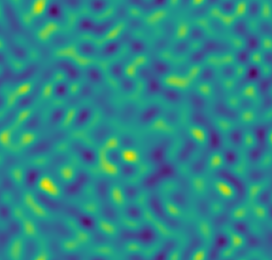
\includegraphics[interpolate=true,width=2.720000in,height=2.600000in]{burgers_solution_0.1-img0.png}}%
\end{pgfscope}%
\begin{pgfscope}%
\pgfsetbuttcap%
\pgfsetroundjoin%
\definecolor{currentfill}{rgb}{0.000000,0.000000,0.000000}%
\pgfsetfillcolor{currentfill}%
\pgfsetlinewidth{0.803000pt}%
\definecolor{currentstroke}{rgb}{0.000000,0.000000,0.000000}%
\pgfsetstrokecolor{currentstroke}%
\pgfsetdash{}{0pt}%
\pgfsys@defobject{currentmarker}{\pgfqpoint{0.000000in}{-0.048611in}}{\pgfqpoint{0.000000in}{0.000000in}}{%
\pgfpathmoveto{\pgfqpoint{0.000000in}{0.000000in}}%
\pgfpathlineto{\pgfqpoint{0.000000in}{-0.048611in}}%
\pgfusepath{stroke,fill}%
}%
\begin{pgfscope}%
\pgfsys@transformshift{0.350969in}{0.300188in}%
\pgfsys@useobject{currentmarker}{}%
\end{pgfscope}%
\end{pgfscope}%
\begin{pgfscope}%
\definecolor{textcolor}{rgb}{0.000000,0.000000,0.000000}%
\pgfsetstrokecolor{textcolor}%
\pgfsetfillcolor{textcolor}%
\pgftext[x=0.350969in,y=0.202965in,,top]{\color{textcolor}{\rmfamily\fontsize{12.000000}{14.400000}\selectfont\catcode`\^=\active\def^{\ifmmode\sp\else\^{}\fi}\catcode`\%=\active\def%{\%}0.0}}%
\end{pgfscope}%
\begin{pgfscope}%
\pgfsetbuttcap%
\pgfsetroundjoin%
\definecolor{currentfill}{rgb}{0.000000,0.000000,0.000000}%
\pgfsetfillcolor{currentfill}%
\pgfsetlinewidth{0.803000pt}%
\definecolor{currentstroke}{rgb}{0.000000,0.000000,0.000000}%
\pgfsetstrokecolor{currentstroke}%
\pgfsetdash{}{0pt}%
\pgfsys@defobject{currentmarker}{\pgfqpoint{0.000000in}{-0.048611in}}{\pgfqpoint{0.000000in}{0.000000in}}{%
\pgfpathmoveto{\pgfqpoint{0.000000in}{0.000000in}}%
\pgfpathlineto{\pgfqpoint{0.000000in}{-0.048611in}}%
\pgfusepath{stroke,fill}%
}%
\begin{pgfscope}%
\pgfsys@transformshift{1.028600in}{0.300188in}%
\pgfsys@useobject{currentmarker}{}%
\end{pgfscope}%
\end{pgfscope}%
\begin{pgfscope}%
\definecolor{textcolor}{rgb}{0.000000,0.000000,0.000000}%
\pgfsetstrokecolor{textcolor}%
\pgfsetfillcolor{textcolor}%
\pgftext[x=1.028600in,y=0.202965in,,top]{\color{textcolor}{\rmfamily\fontsize{12.000000}{14.400000}\selectfont\catcode`\^=\active\def^{\ifmmode\sp\else\^{}\fi}\catcode`\%=\active\def%{\%}0.5}}%
\end{pgfscope}%
\begin{pgfscope}%
\pgfsetbuttcap%
\pgfsetroundjoin%
\definecolor{currentfill}{rgb}{0.000000,0.000000,0.000000}%
\pgfsetfillcolor{currentfill}%
\pgfsetlinewidth{0.803000pt}%
\definecolor{currentstroke}{rgb}{0.000000,0.000000,0.000000}%
\pgfsetstrokecolor{currentstroke}%
\pgfsetdash{}{0pt}%
\pgfsys@defobject{currentmarker}{\pgfqpoint{0.000000in}{-0.048611in}}{\pgfqpoint{0.000000in}{0.000000in}}{%
\pgfpathmoveto{\pgfqpoint{0.000000in}{0.000000in}}%
\pgfpathlineto{\pgfqpoint{0.000000in}{-0.048611in}}%
\pgfusepath{stroke,fill}%
}%
\begin{pgfscope}%
\pgfsys@transformshift{1.706232in}{0.300188in}%
\pgfsys@useobject{currentmarker}{}%
\end{pgfscope}%
\end{pgfscope}%
\begin{pgfscope}%
\definecolor{textcolor}{rgb}{0.000000,0.000000,0.000000}%
\pgfsetstrokecolor{textcolor}%
\pgfsetfillcolor{textcolor}%
\pgftext[x=1.706232in,y=0.202965in,,top]{\color{textcolor}{\rmfamily\fontsize{12.000000}{14.400000}\selectfont\catcode`\^=\active\def^{\ifmmode\sp\else\^{}\fi}\catcode`\%=\active\def%{\%}1.0}}%
\end{pgfscope}%
\begin{pgfscope}%
\pgfsetbuttcap%
\pgfsetroundjoin%
\definecolor{currentfill}{rgb}{0.000000,0.000000,0.000000}%
\pgfsetfillcolor{currentfill}%
\pgfsetlinewidth{0.803000pt}%
\definecolor{currentstroke}{rgb}{0.000000,0.000000,0.000000}%
\pgfsetstrokecolor{currentstroke}%
\pgfsetdash{}{0pt}%
\pgfsys@defobject{currentmarker}{\pgfqpoint{0.000000in}{-0.048611in}}{\pgfqpoint{0.000000in}{0.000000in}}{%
\pgfpathmoveto{\pgfqpoint{0.000000in}{0.000000in}}%
\pgfpathlineto{\pgfqpoint{0.000000in}{-0.048611in}}%
\pgfusepath{stroke,fill}%
}%
\begin{pgfscope}%
\pgfsys@transformshift{2.383863in}{0.300188in}%
\pgfsys@useobject{currentmarker}{}%
\end{pgfscope}%
\end{pgfscope}%
\begin{pgfscope}%
\definecolor{textcolor}{rgb}{0.000000,0.000000,0.000000}%
\pgfsetstrokecolor{textcolor}%
\pgfsetfillcolor{textcolor}%
\pgftext[x=2.383863in,y=0.202965in,,top]{\color{textcolor}{\rmfamily\fontsize{12.000000}{14.400000}\selectfont\catcode`\^=\active\def^{\ifmmode\sp\else\^{}\fi}\catcode`\%=\active\def%{\%}1.5}}%
\end{pgfscope}%
\begin{pgfscope}%
\pgfsetbuttcap%
\pgfsetroundjoin%
\definecolor{currentfill}{rgb}{0.000000,0.000000,0.000000}%
\pgfsetfillcolor{currentfill}%
\pgfsetlinewidth{0.803000pt}%
\definecolor{currentstroke}{rgb}{0.000000,0.000000,0.000000}%
\pgfsetstrokecolor{currentstroke}%
\pgfsetdash{}{0pt}%
\pgfsys@defobject{currentmarker}{\pgfqpoint{0.000000in}{-0.048611in}}{\pgfqpoint{0.000000in}{0.000000in}}{%
\pgfpathmoveto{\pgfqpoint{0.000000in}{0.000000in}}%
\pgfpathlineto{\pgfqpoint{0.000000in}{-0.048611in}}%
\pgfusepath{stroke,fill}%
}%
\begin{pgfscope}%
\pgfsys@transformshift{3.061494in}{0.300188in}%
\pgfsys@useobject{currentmarker}{}%
\end{pgfscope}%
\end{pgfscope}%
\begin{pgfscope}%
\definecolor{textcolor}{rgb}{0.000000,0.000000,0.000000}%
\pgfsetstrokecolor{textcolor}%
\pgfsetfillcolor{textcolor}%
\pgftext[x=3.061494in,y=0.202965in,,top]{\color{textcolor}{\rmfamily\fontsize{12.000000}{14.400000}\selectfont\catcode`\^=\active\def^{\ifmmode\sp\else\^{}\fi}\catcode`\%=\active\def%{\%}2.0}}%
\end{pgfscope}%
\begin{pgfscope}%
\pgfsetbuttcap%
\pgfsetroundjoin%
\definecolor{currentfill}{rgb}{0.000000,0.000000,0.000000}%
\pgfsetfillcolor{currentfill}%
\pgfsetlinewidth{0.803000pt}%
\definecolor{currentstroke}{rgb}{0.000000,0.000000,0.000000}%
\pgfsetstrokecolor{currentstroke}%
\pgfsetdash{}{0pt}%
\pgfsys@defobject{currentmarker}{\pgfqpoint{-0.048611in}{0.000000in}}{\pgfqpoint{-0.000000in}{0.000000in}}{%
\pgfpathmoveto{\pgfqpoint{-0.000000in}{0.000000in}}%
\pgfpathlineto{\pgfqpoint{-0.048611in}{0.000000in}}%
\pgfusepath{stroke,fill}%
}%
\begin{pgfscope}%
\pgfsys@transformshift{0.350969in}{0.300188in}%
\pgfsys@useobject{currentmarker}{}%
\end{pgfscope}%
\end{pgfscope}%
\begin{pgfscope}%
\definecolor{textcolor}{rgb}{0.000000,0.000000,0.000000}%
\pgfsetstrokecolor{textcolor}%
\pgfsetfillcolor{textcolor}%
\pgftext[x=0.147708in, y=0.236874in, left, base]{\color{textcolor}{\rmfamily\fontsize{12.000000}{14.400000}\selectfont\catcode`\^=\active\def^{\ifmmode\sp\else\^{}\fi}\catcode`\%=\active\def%{\%}0}}%
\end{pgfscope}%
\begin{pgfscope}%
\pgfsetbuttcap%
\pgfsetroundjoin%
\definecolor{currentfill}{rgb}{0.000000,0.000000,0.000000}%
\pgfsetfillcolor{currentfill}%
\pgfsetlinewidth{0.803000pt}%
\definecolor{currentstroke}{rgb}{0.000000,0.000000,0.000000}%
\pgfsetstrokecolor{currentstroke}%
\pgfsetdash{}{0pt}%
\pgfsys@defobject{currentmarker}{\pgfqpoint{-0.048611in}{0.000000in}}{\pgfqpoint{-0.000000in}{0.000000in}}{%
\pgfpathmoveto{\pgfqpoint{-0.000000in}{0.000000in}}%
\pgfpathlineto{\pgfqpoint{-0.048611in}{0.000000in}}%
\pgfusepath{stroke,fill}%
}%
\begin{pgfscope}%
\pgfsys@transformshift{0.350969in}{0.819153in}%
\pgfsys@useobject{currentmarker}{}%
\end{pgfscope}%
\end{pgfscope}%
\begin{pgfscope}%
\definecolor{textcolor}{rgb}{0.000000,0.000000,0.000000}%
\pgfsetstrokecolor{textcolor}%
\pgfsetfillcolor{textcolor}%
\pgftext[x=0.147708in, y=0.755840in, left, base]{\color{textcolor}{\rmfamily\fontsize{12.000000}{14.400000}\selectfont\catcode`\^=\active\def^{\ifmmode\sp\else\^{}\fi}\catcode`\%=\active\def%{\%}2}}%
\end{pgfscope}%
\begin{pgfscope}%
\pgfsetbuttcap%
\pgfsetroundjoin%
\definecolor{currentfill}{rgb}{0.000000,0.000000,0.000000}%
\pgfsetfillcolor{currentfill}%
\pgfsetlinewidth{0.803000pt}%
\definecolor{currentstroke}{rgb}{0.000000,0.000000,0.000000}%
\pgfsetstrokecolor{currentstroke}%
\pgfsetdash{}{0pt}%
\pgfsys@defobject{currentmarker}{\pgfqpoint{-0.048611in}{0.000000in}}{\pgfqpoint{-0.000000in}{0.000000in}}{%
\pgfpathmoveto{\pgfqpoint{-0.000000in}{0.000000in}}%
\pgfpathlineto{\pgfqpoint{-0.048611in}{0.000000in}}%
\pgfusepath{stroke,fill}%
}%
\begin{pgfscope}%
\pgfsys@transformshift{0.350969in}{1.338119in}%
\pgfsys@useobject{currentmarker}{}%
\end{pgfscope}%
\end{pgfscope}%
\begin{pgfscope}%
\definecolor{textcolor}{rgb}{0.000000,0.000000,0.000000}%
\pgfsetstrokecolor{textcolor}%
\pgfsetfillcolor{textcolor}%
\pgftext[x=0.147708in, y=1.274805in, left, base]{\color{textcolor}{\rmfamily\fontsize{12.000000}{14.400000}\selectfont\catcode`\^=\active\def^{\ifmmode\sp\else\^{}\fi}\catcode`\%=\active\def%{\%}4}}%
\end{pgfscope}%
\begin{pgfscope}%
\pgfsetbuttcap%
\pgfsetroundjoin%
\definecolor{currentfill}{rgb}{0.000000,0.000000,0.000000}%
\pgfsetfillcolor{currentfill}%
\pgfsetlinewidth{0.803000pt}%
\definecolor{currentstroke}{rgb}{0.000000,0.000000,0.000000}%
\pgfsetstrokecolor{currentstroke}%
\pgfsetdash{}{0pt}%
\pgfsys@defobject{currentmarker}{\pgfqpoint{-0.048611in}{0.000000in}}{\pgfqpoint{-0.000000in}{0.000000in}}{%
\pgfpathmoveto{\pgfqpoint{-0.000000in}{0.000000in}}%
\pgfpathlineto{\pgfqpoint{-0.048611in}{0.000000in}}%
\pgfusepath{stroke,fill}%
}%
\begin{pgfscope}%
\pgfsys@transformshift{0.350969in}{1.857085in}%
\pgfsys@useobject{currentmarker}{}%
\end{pgfscope}%
\end{pgfscope}%
\begin{pgfscope}%
\definecolor{textcolor}{rgb}{0.000000,0.000000,0.000000}%
\pgfsetstrokecolor{textcolor}%
\pgfsetfillcolor{textcolor}%
\pgftext[x=0.147708in, y=1.793771in, left, base]{\color{textcolor}{\rmfamily\fontsize{12.000000}{14.400000}\selectfont\catcode`\^=\active\def^{\ifmmode\sp\else\^{}\fi}\catcode`\%=\active\def%{\%}6}}%
\end{pgfscope}%
\begin{pgfscope}%
\pgfsetbuttcap%
\pgfsetroundjoin%
\definecolor{currentfill}{rgb}{0.000000,0.000000,0.000000}%
\pgfsetfillcolor{currentfill}%
\pgfsetlinewidth{0.803000pt}%
\definecolor{currentstroke}{rgb}{0.000000,0.000000,0.000000}%
\pgfsetstrokecolor{currentstroke}%
\pgfsetdash{}{0pt}%
\pgfsys@defobject{currentmarker}{\pgfqpoint{-0.048611in}{0.000000in}}{\pgfqpoint{-0.000000in}{0.000000in}}{%
\pgfpathmoveto{\pgfqpoint{-0.000000in}{0.000000in}}%
\pgfpathlineto{\pgfqpoint{-0.048611in}{0.000000in}}%
\pgfusepath{stroke,fill}%
}%
\begin{pgfscope}%
\pgfsys@transformshift{0.350969in}{2.376050in}%
\pgfsys@useobject{currentmarker}{}%
\end{pgfscope}%
\end{pgfscope}%
\begin{pgfscope}%
\definecolor{textcolor}{rgb}{0.000000,0.000000,0.000000}%
\pgfsetstrokecolor{textcolor}%
\pgfsetfillcolor{textcolor}%
\pgftext[x=0.147708in, y=2.312737in, left, base]{\color{textcolor}{\rmfamily\fontsize{12.000000}{14.400000}\selectfont\catcode`\^=\active\def^{\ifmmode\sp\else\^{}\fi}\catcode`\%=\active\def%{\%}8}}%
\end{pgfscope}%
\begin{pgfscope}%
\pgfsetbuttcap%
\pgfsetroundjoin%
\definecolor{currentfill}{rgb}{0.000000,0.000000,0.000000}%
\pgfsetfillcolor{currentfill}%
\pgfsetlinewidth{0.803000pt}%
\definecolor{currentstroke}{rgb}{0.000000,0.000000,0.000000}%
\pgfsetstrokecolor{currentstroke}%
\pgfsetdash{}{0pt}%
\pgfsys@defobject{currentmarker}{\pgfqpoint{-0.048611in}{0.000000in}}{\pgfqpoint{-0.000000in}{0.000000in}}{%
\pgfpathmoveto{\pgfqpoint{-0.000000in}{0.000000in}}%
\pgfpathlineto{\pgfqpoint{-0.048611in}{0.000000in}}%
\pgfusepath{stroke,fill}%
}%
\begin{pgfscope}%
\pgfsys@transformshift{0.350969in}{2.895016in}%
\pgfsys@useobject{currentmarker}{}%
\end{pgfscope}%
\end{pgfscope}%
\begin{pgfscope}%
\definecolor{textcolor}{rgb}{0.000000,0.000000,0.000000}%
\pgfsetstrokecolor{textcolor}%
\pgfsetfillcolor{textcolor}%
\pgftext[x=0.041670in, y=2.831702in, left, base]{\color{textcolor}{\rmfamily\fontsize{12.000000}{14.400000}\selectfont\catcode`\^=\active\def^{\ifmmode\sp\else\^{}\fi}\catcode`\%=\active\def%{\%}10}}%
\end{pgfscope}%
\begin{pgfscope}%
\pgfsetrectcap%
\pgfsetmiterjoin%
\pgfsetlinewidth{0.803000pt}%
\definecolor{currentstroke}{rgb}{0.000000,0.000000,0.000000}%
\pgfsetstrokecolor{currentstroke}%
\pgfsetdash{}{0pt}%
\pgfpathmoveto{\pgfqpoint{0.350969in}{0.300188in}}%
\pgfpathlineto{\pgfqpoint{0.350969in}{2.895016in}}%
\pgfusepath{stroke}%
\end{pgfscope}%
\begin{pgfscope}%
\pgfsetrectcap%
\pgfsetmiterjoin%
\pgfsetlinewidth{0.803000pt}%
\definecolor{currentstroke}{rgb}{0.000000,0.000000,0.000000}%
\pgfsetstrokecolor{currentstroke}%
\pgfsetdash{}{0pt}%
\pgfpathmoveto{\pgfqpoint{3.061494in}{0.300188in}}%
\pgfpathlineto{\pgfqpoint{3.061494in}{2.895016in}}%
\pgfusepath{stroke}%
\end{pgfscope}%
\begin{pgfscope}%
\pgfsetrectcap%
\pgfsetmiterjoin%
\pgfsetlinewidth{0.803000pt}%
\definecolor{currentstroke}{rgb}{0.000000,0.000000,0.000000}%
\pgfsetstrokecolor{currentstroke}%
\pgfsetdash{}{0pt}%
\pgfpathmoveto{\pgfqpoint{0.350969in}{0.300188in}}%
\pgfpathlineto{\pgfqpoint{3.061494in}{0.300188in}}%
\pgfusepath{stroke}%
\end{pgfscope}%
\begin{pgfscope}%
\pgfsetrectcap%
\pgfsetmiterjoin%
\pgfsetlinewidth{0.803000pt}%
\definecolor{currentstroke}{rgb}{0.000000,0.000000,0.000000}%
\pgfsetstrokecolor{currentstroke}%
\pgfsetdash{}{0pt}%
\pgfpathmoveto{\pgfqpoint{0.350969in}{2.895016in}}%
\pgfpathlineto{\pgfqpoint{3.061494in}{2.895016in}}%
\pgfusepath{stroke}%
\end{pgfscope}%
\begin{pgfscope}%
\pgfsetbuttcap%
\pgfsetmiterjoin%
\pgfsetlinewidth{0.000000pt}%
\definecolor{currentstroke}{rgb}{0.000000,0.000000,0.000000}%
\pgfsetstrokecolor{currentstroke}%
\pgfsetstrokeopacity{0.000000}%
\pgfsetdash{}{0pt}%
\pgfpathmoveto{\pgfqpoint{3.329548in}{0.300188in}}%
\pgfpathlineto{\pgfqpoint{3.459290in}{0.300188in}}%
\pgfpathlineto{\pgfqpoint{3.459290in}{2.895016in}}%
\pgfpathlineto{\pgfqpoint{3.329548in}{2.895016in}}%
\pgfpathlineto{\pgfqpoint{3.329548in}{0.300188in}}%
\pgfpathclose%
\pgfusepath{}%
\end{pgfscope}%
\begin{pgfscope}%
\pgfsys@transformshift{3.330000in}{0.300000in}%
\pgftext[left,bottom]{
\includegraphics[interpolate=true,width=0.130000in,height=2.600000in]{burgers_solution_0.1-img1.png}}%
\end{pgfscope}%
\begin{pgfscope}%
\pgfsetbuttcap%
\pgfsetroundjoin%
\definecolor{currentfill}{rgb}{0.000000,0.000000,0.000000}%
\pgfsetfillcolor{currentfill}%
\pgfsetlinewidth{0.803000pt}%
\definecolor{currentstroke}{rgb}{0.000000,0.000000,0.000000}%
\pgfsetstrokecolor{currentstroke}%
\pgfsetdash{}{0pt}%
\pgfsys@defobject{currentmarker}{\pgfqpoint{0.000000in}{0.000000in}}{\pgfqpoint{0.048611in}{0.000000in}}{%
\pgfpathmoveto{\pgfqpoint{0.000000in}{0.000000in}}%
\pgfpathlineto{\pgfqpoint{0.048611in}{0.000000in}}%
\pgfusepath{stroke,fill}%
}%
\begin{pgfscope}%
\pgfsys@transformshift{3.459290in}{0.840201in}%
\pgfsys@useobject{currentmarker}{}%
\end{pgfscope}%
\end{pgfscope}%
\begin{pgfscope}%
\definecolor{textcolor}{rgb}{0.000000,0.000000,0.000000}%
\pgfsetstrokecolor{textcolor}%
\pgfsetfillcolor{textcolor}%
\pgftext[x=3.556512in, y=0.776887in, left, base]{\color{textcolor}{\rmfamily\fontsize{12.000000}{14.400000}\selectfont\catcode`\^=\active\def^{\ifmmode\sp\else\^{}\fi}\catcode`\%=\active\def%{\%}\ensuremath{-}0.5}}%
\end{pgfscope}%
\begin{pgfscope}%
\pgfsetbuttcap%
\pgfsetroundjoin%
\definecolor{currentfill}{rgb}{0.000000,0.000000,0.000000}%
\pgfsetfillcolor{currentfill}%
\pgfsetlinewidth{0.803000pt}%
\definecolor{currentstroke}{rgb}{0.000000,0.000000,0.000000}%
\pgfsetstrokecolor{currentstroke}%
\pgfsetdash{}{0pt}%
\pgfsys@defobject{currentmarker}{\pgfqpoint{0.000000in}{0.000000in}}{\pgfqpoint{0.048611in}{0.000000in}}{%
\pgfpathmoveto{\pgfqpoint{0.000000in}{0.000000in}}%
\pgfpathlineto{\pgfqpoint{0.048611in}{0.000000in}}%
\pgfusepath{stroke,fill}%
}%
\begin{pgfscope}%
\pgfsys@transformshift{3.459290in}{1.494629in}%
\pgfsys@useobject{currentmarker}{}%
\end{pgfscope}%
\end{pgfscope}%
\begin{pgfscope}%
\definecolor{textcolor}{rgb}{0.000000,0.000000,0.000000}%
\pgfsetstrokecolor{textcolor}%
\pgfsetfillcolor{textcolor}%
\pgftext[x=3.556512in, y=1.431315in, left, base]{\color{textcolor}{\rmfamily\fontsize{12.000000}{14.400000}\selectfont\catcode`\^=\active\def^{\ifmmode\sp\else\^{}\fi}\catcode`\%=\active\def%{\%}0.0}}%
\end{pgfscope}%
\begin{pgfscope}%
\pgfsetbuttcap%
\pgfsetroundjoin%
\definecolor{currentfill}{rgb}{0.000000,0.000000,0.000000}%
\pgfsetfillcolor{currentfill}%
\pgfsetlinewidth{0.803000pt}%
\definecolor{currentstroke}{rgb}{0.000000,0.000000,0.000000}%
\pgfsetstrokecolor{currentstroke}%
\pgfsetdash{}{0pt}%
\pgfsys@defobject{currentmarker}{\pgfqpoint{0.000000in}{0.000000in}}{\pgfqpoint{0.048611in}{0.000000in}}{%
\pgfpathmoveto{\pgfqpoint{0.000000in}{0.000000in}}%
\pgfpathlineto{\pgfqpoint{0.048611in}{0.000000in}}%
\pgfusepath{stroke,fill}%
}%
\begin{pgfscope}%
\pgfsys@transformshift{3.459290in}{2.149056in}%
\pgfsys@useobject{currentmarker}{}%
\end{pgfscope}%
\end{pgfscope}%
\begin{pgfscope}%
\definecolor{textcolor}{rgb}{0.000000,0.000000,0.000000}%
\pgfsetstrokecolor{textcolor}%
\pgfsetfillcolor{textcolor}%
\pgftext[x=3.556512in, y=2.085742in, left, base]{\color{textcolor}{\rmfamily\fontsize{12.000000}{14.400000}\selectfont\catcode`\^=\active\def^{\ifmmode\sp\else\^{}\fi}\catcode`\%=\active\def%{\%}0.5}}%
\end{pgfscope}%
\begin{pgfscope}%
\pgfsetbuttcap%
\pgfsetroundjoin%
\definecolor{currentfill}{rgb}{0.000000,0.000000,0.000000}%
\pgfsetfillcolor{currentfill}%
\pgfsetlinewidth{0.803000pt}%
\definecolor{currentstroke}{rgb}{0.000000,0.000000,0.000000}%
\pgfsetstrokecolor{currentstroke}%
\pgfsetdash{}{0pt}%
\pgfsys@defobject{currentmarker}{\pgfqpoint{0.000000in}{0.000000in}}{\pgfqpoint{0.048611in}{0.000000in}}{%
\pgfpathmoveto{\pgfqpoint{0.000000in}{0.000000in}}%
\pgfpathlineto{\pgfqpoint{0.048611in}{0.000000in}}%
\pgfusepath{stroke,fill}%
}%
\begin{pgfscope}%
\pgfsys@transformshift{3.459290in}{2.803483in}%
\pgfsys@useobject{currentmarker}{}%
\end{pgfscope}%
\end{pgfscope}%
\begin{pgfscope}%
\definecolor{textcolor}{rgb}{0.000000,0.000000,0.000000}%
\pgfsetstrokecolor{textcolor}%
\pgfsetfillcolor{textcolor}%
\pgftext[x=3.556512in, y=2.740170in, left, base]{\color{textcolor}{\rmfamily\fontsize{12.000000}{14.400000}\selectfont\catcode`\^=\active\def^{\ifmmode\sp\else\^{}\fi}\catcode`\%=\active\def%{\%}1.0}}%
\end{pgfscope}%
\begin{pgfscope}%
\pgfsetrectcap%
\pgfsetmiterjoin%
\pgfsetlinewidth{0.803000pt}%
\definecolor{currentstroke}{rgb}{0.000000,0.000000,0.000000}%
\pgfsetstrokecolor{currentstroke}%
\pgfsetdash{}{0pt}%
\pgfpathmoveto{\pgfqpoint{3.329548in}{0.300188in}}%
\pgfpathlineto{\pgfqpoint{3.394419in}{0.300188in}}%
\pgfpathlineto{\pgfqpoint{3.459290in}{0.300188in}}%
\pgfpathlineto{\pgfqpoint{3.459290in}{2.895016in}}%
\pgfpathlineto{\pgfqpoint{3.394419in}{2.895016in}}%
\pgfpathlineto{\pgfqpoint{3.329548in}{2.895016in}}%
\pgfpathlineto{\pgfqpoint{3.329548in}{0.300188in}}%
\pgfpathclose%
\pgfusepath{stroke}%
\end{pgfscope}%
\end{pgfpicture}%
\makeatother%
\endgroup%

    \end{adjustbox}
    \caption{Solution function for \(\nu=0.1\).}\label{fig:burgers_solution_0.1}
  \end{subfigure}
  \begin{subfigure}{0.49\linewidth}
    \begin{adjustbox}{width=\linewidth}
      \begingroup%
\makeatletter%
\begin{pgfpicture}%
\pgfpathrectangle{\pgfpointorigin}{\pgfqpoint{4.000000in}{3.000000in}}%
\pgfusepath{use as bounding box, clip}%
\begin{pgfscope}%
\pgfsetbuttcap%
\pgfsetmiterjoin%
\pgfsetlinewidth{0.000000pt}%
\definecolor{currentstroke}{rgb}{0.000000,0.000000,0.000000}%
\pgfsetstrokecolor{currentstroke}%
\pgfsetstrokeopacity{0.000000}%
\pgfsetdash{}{0pt}%
\pgfpathmoveto{\pgfqpoint{0.000000in}{0.000000in}}%
\pgfpathlineto{\pgfqpoint{4.000000in}{0.000000in}}%
\pgfpathlineto{\pgfqpoint{4.000000in}{3.000000in}}%
\pgfpathlineto{\pgfqpoint{0.000000in}{3.000000in}}%
\pgfpathlineto{\pgfqpoint{0.000000in}{0.000000in}}%
\pgfpathclose%
\pgfusepath{}%
\end{pgfscope}%
\begin{pgfscope}%
\pgfsetbuttcap%
\pgfsetmiterjoin%
\pgfsetlinewidth{0.000000pt}%
\definecolor{currentstroke}{rgb}{0.000000,0.000000,0.000000}%
\pgfsetstrokecolor{currentstroke}%
\pgfsetstrokeopacity{0.000000}%
\pgfsetdash{}{0pt}%
\pgfpathmoveto{\pgfqpoint{0.567820in}{0.517039in}}%
\pgfpathlineto{\pgfqpoint{3.233703in}{0.517039in}}%
\pgfpathlineto{\pgfqpoint{3.233703in}{2.895016in}}%
\pgfpathlineto{\pgfqpoint{0.567820in}{2.895016in}}%
\pgfpathlineto{\pgfqpoint{0.567820in}{0.517039in}}%
\pgfpathclose%
\pgfusepath{}%
\end{pgfscope}%
\begin{pgfscope}%
\pgfpathrectangle{\pgfqpoint{0.567820in}{0.517039in}}{\pgfqpoint{2.665883in}{2.377978in}}%
\pgfusepath{clip}%
\pgfsys@transformshift{0.567820in}{0.517039in}%
\pgftext[left,bottom]{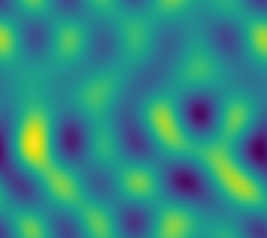
\includegraphics[interpolate=true,width=2.670000in,height=2.380000in]{burgers_forcing_0.1-img0.png}}%
\end{pgfscope}%
\begin{pgfscope}%
\pgfsetbuttcap%
\pgfsetroundjoin%
\definecolor{currentfill}{rgb}{0.000000,0.000000,0.000000}%
\pgfsetfillcolor{currentfill}%
\pgfsetlinewidth{0.803000pt}%
\definecolor{currentstroke}{rgb}{0.000000,0.000000,0.000000}%
\pgfsetstrokecolor{currentstroke}%
\pgfsetdash{}{0pt}%
\pgfsys@defobject{currentmarker}{\pgfqpoint{0.000000in}{-0.048611in}}{\pgfqpoint{0.000000in}{0.000000in}}{%
\pgfpathmoveto{\pgfqpoint{0.000000in}{0.000000in}}%
\pgfpathlineto{\pgfqpoint{0.000000in}{-0.048611in}}%
\pgfusepath{stroke,fill}%
}%
\begin{pgfscope}%
\pgfsys@transformshift{0.567820in}{0.517039in}%
\pgfsys@useobject{currentmarker}{}%
\end{pgfscope}%
\end{pgfscope}%
\begin{pgfscope}%
\definecolor{textcolor}{rgb}{0.000000,0.000000,0.000000}%
\pgfsetstrokecolor{textcolor}%
\pgfsetfillcolor{textcolor}%
\pgftext[x=0.567820in,y=0.419816in,,top]{\color{textcolor}\rmfamily\fontsize{12.000000}{14.400000}\selectfont 0.0}%
\end{pgfscope}%
\begin{pgfscope}%
\pgfsetbuttcap%
\pgfsetroundjoin%
\definecolor{currentfill}{rgb}{0.000000,0.000000,0.000000}%
\pgfsetfillcolor{currentfill}%
\pgfsetlinewidth{0.803000pt}%
\definecolor{currentstroke}{rgb}{0.000000,0.000000,0.000000}%
\pgfsetstrokecolor{currentstroke}%
\pgfsetdash{}{0pt}%
\pgfsys@defobject{currentmarker}{\pgfqpoint{0.000000in}{-0.048611in}}{\pgfqpoint{0.000000in}{0.000000in}}{%
\pgfpathmoveto{\pgfqpoint{0.000000in}{0.000000in}}%
\pgfpathlineto{\pgfqpoint{0.000000in}{-0.048611in}}%
\pgfusepath{stroke,fill}%
}%
\begin{pgfscope}%
\pgfsys@transformshift{1.234291in}{0.517039in}%
\pgfsys@useobject{currentmarker}{}%
\end{pgfscope}%
\end{pgfscope}%
\begin{pgfscope}%
\definecolor{textcolor}{rgb}{0.000000,0.000000,0.000000}%
\pgfsetstrokecolor{textcolor}%
\pgfsetfillcolor{textcolor}%
\pgftext[x=1.234291in,y=0.419816in,,top]{\color{textcolor}\rmfamily\fontsize{12.000000}{14.400000}\selectfont 0.5}%
\end{pgfscope}%
\begin{pgfscope}%
\pgfsetbuttcap%
\pgfsetroundjoin%
\definecolor{currentfill}{rgb}{0.000000,0.000000,0.000000}%
\pgfsetfillcolor{currentfill}%
\pgfsetlinewidth{0.803000pt}%
\definecolor{currentstroke}{rgb}{0.000000,0.000000,0.000000}%
\pgfsetstrokecolor{currentstroke}%
\pgfsetdash{}{0pt}%
\pgfsys@defobject{currentmarker}{\pgfqpoint{0.000000in}{-0.048611in}}{\pgfqpoint{0.000000in}{0.000000in}}{%
\pgfpathmoveto{\pgfqpoint{0.000000in}{0.000000in}}%
\pgfpathlineto{\pgfqpoint{0.000000in}{-0.048611in}}%
\pgfusepath{stroke,fill}%
}%
\begin{pgfscope}%
\pgfsys@transformshift{1.900762in}{0.517039in}%
\pgfsys@useobject{currentmarker}{}%
\end{pgfscope}%
\end{pgfscope}%
\begin{pgfscope}%
\definecolor{textcolor}{rgb}{0.000000,0.000000,0.000000}%
\pgfsetstrokecolor{textcolor}%
\pgfsetfillcolor{textcolor}%
\pgftext[x=1.900762in,y=0.419816in,,top]{\color{textcolor}\rmfamily\fontsize{12.000000}{14.400000}\selectfont 1.0}%
\end{pgfscope}%
\begin{pgfscope}%
\pgfsetbuttcap%
\pgfsetroundjoin%
\definecolor{currentfill}{rgb}{0.000000,0.000000,0.000000}%
\pgfsetfillcolor{currentfill}%
\pgfsetlinewidth{0.803000pt}%
\definecolor{currentstroke}{rgb}{0.000000,0.000000,0.000000}%
\pgfsetstrokecolor{currentstroke}%
\pgfsetdash{}{0pt}%
\pgfsys@defobject{currentmarker}{\pgfqpoint{0.000000in}{-0.048611in}}{\pgfqpoint{0.000000in}{0.000000in}}{%
\pgfpathmoveto{\pgfqpoint{0.000000in}{0.000000in}}%
\pgfpathlineto{\pgfqpoint{0.000000in}{-0.048611in}}%
\pgfusepath{stroke,fill}%
}%
\begin{pgfscope}%
\pgfsys@transformshift{2.567232in}{0.517039in}%
\pgfsys@useobject{currentmarker}{}%
\end{pgfscope}%
\end{pgfscope}%
\begin{pgfscope}%
\definecolor{textcolor}{rgb}{0.000000,0.000000,0.000000}%
\pgfsetstrokecolor{textcolor}%
\pgfsetfillcolor{textcolor}%
\pgftext[x=2.567232in,y=0.419816in,,top]{\color{textcolor}\rmfamily\fontsize{12.000000}{14.400000}\selectfont 1.5}%
\end{pgfscope}%
\begin{pgfscope}%
\pgfsetbuttcap%
\pgfsetroundjoin%
\definecolor{currentfill}{rgb}{0.000000,0.000000,0.000000}%
\pgfsetfillcolor{currentfill}%
\pgfsetlinewidth{0.803000pt}%
\definecolor{currentstroke}{rgb}{0.000000,0.000000,0.000000}%
\pgfsetstrokecolor{currentstroke}%
\pgfsetdash{}{0pt}%
\pgfsys@defobject{currentmarker}{\pgfqpoint{0.000000in}{-0.048611in}}{\pgfqpoint{0.000000in}{0.000000in}}{%
\pgfpathmoveto{\pgfqpoint{0.000000in}{0.000000in}}%
\pgfpathlineto{\pgfqpoint{0.000000in}{-0.048611in}}%
\pgfusepath{stroke,fill}%
}%
\begin{pgfscope}%
\pgfsys@transformshift{3.233703in}{0.517039in}%
\pgfsys@useobject{currentmarker}{}%
\end{pgfscope}%
\end{pgfscope}%
\begin{pgfscope}%
\definecolor{textcolor}{rgb}{0.000000,0.000000,0.000000}%
\pgfsetstrokecolor{textcolor}%
\pgfsetfillcolor{textcolor}%
\pgftext[x=3.233703in,y=0.419816in,,top]{\color{textcolor}\rmfamily\fontsize{12.000000}{14.400000}\selectfont 2.0}%
\end{pgfscope}%
\begin{pgfscope}%
\definecolor{textcolor}{rgb}{0.000000,0.000000,0.000000}%
\pgfsetstrokecolor{textcolor}%
\pgfsetfillcolor{textcolor}%
\pgftext[x=1.900762in,y=0.202965in,,top]{\color{textcolor}\rmfamily\fontsize{12.000000}{14.400000}\selectfont Space}%
\end{pgfscope}%
\begin{pgfscope}%
\pgfsetbuttcap%
\pgfsetroundjoin%
\definecolor{currentfill}{rgb}{0.000000,0.000000,0.000000}%
\pgfsetfillcolor{currentfill}%
\pgfsetlinewidth{0.803000pt}%
\definecolor{currentstroke}{rgb}{0.000000,0.000000,0.000000}%
\pgfsetstrokecolor{currentstroke}%
\pgfsetdash{}{0pt}%
\pgfsys@defobject{currentmarker}{\pgfqpoint{-0.048611in}{0.000000in}}{\pgfqpoint{-0.000000in}{0.000000in}}{%
\pgfpathmoveto{\pgfqpoint{-0.000000in}{0.000000in}}%
\pgfpathlineto{\pgfqpoint{-0.048611in}{0.000000in}}%
\pgfusepath{stroke,fill}%
}%
\begin{pgfscope}%
\pgfsys@transformshift{0.567820in}{0.517039in}%
\pgfsys@useobject{currentmarker}{}%
\end{pgfscope}%
\end{pgfscope}%
\begin{pgfscope}%
\definecolor{textcolor}{rgb}{0.000000,0.000000,0.000000}%
\pgfsetstrokecolor{textcolor}%
\pgfsetfillcolor{textcolor}%
\pgftext[x=0.364559in, y=0.453725in, left, base]{\color{textcolor}\rmfamily\fontsize{12.000000}{14.400000}\selectfont 0}%
\end{pgfscope}%
\begin{pgfscope}%
\pgfsetbuttcap%
\pgfsetroundjoin%
\definecolor{currentfill}{rgb}{0.000000,0.000000,0.000000}%
\pgfsetfillcolor{currentfill}%
\pgfsetlinewidth{0.803000pt}%
\definecolor{currentstroke}{rgb}{0.000000,0.000000,0.000000}%
\pgfsetstrokecolor{currentstroke}%
\pgfsetdash{}{0pt}%
\pgfsys@defobject{currentmarker}{\pgfqpoint{-0.048611in}{0.000000in}}{\pgfqpoint{-0.000000in}{0.000000in}}{%
\pgfpathmoveto{\pgfqpoint{-0.000000in}{0.000000in}}%
\pgfpathlineto{\pgfqpoint{-0.048611in}{0.000000in}}%
\pgfusepath{stroke,fill}%
}%
\begin{pgfscope}%
\pgfsys@transformshift{0.567820in}{0.992634in}%
\pgfsys@useobject{currentmarker}{}%
\end{pgfscope}%
\end{pgfscope}%
\begin{pgfscope}%
\definecolor{textcolor}{rgb}{0.000000,0.000000,0.000000}%
\pgfsetstrokecolor{textcolor}%
\pgfsetfillcolor{textcolor}%
\pgftext[x=0.364559in, y=0.929320in, left, base]{\color{textcolor}\rmfamily\fontsize{12.000000}{14.400000}\selectfont 2}%
\end{pgfscope}%
\begin{pgfscope}%
\pgfsetbuttcap%
\pgfsetroundjoin%
\definecolor{currentfill}{rgb}{0.000000,0.000000,0.000000}%
\pgfsetfillcolor{currentfill}%
\pgfsetlinewidth{0.803000pt}%
\definecolor{currentstroke}{rgb}{0.000000,0.000000,0.000000}%
\pgfsetstrokecolor{currentstroke}%
\pgfsetdash{}{0pt}%
\pgfsys@defobject{currentmarker}{\pgfqpoint{-0.048611in}{0.000000in}}{\pgfqpoint{-0.000000in}{0.000000in}}{%
\pgfpathmoveto{\pgfqpoint{-0.000000in}{0.000000in}}%
\pgfpathlineto{\pgfqpoint{-0.048611in}{0.000000in}}%
\pgfusepath{stroke,fill}%
}%
\begin{pgfscope}%
\pgfsys@transformshift{0.567820in}{1.468230in}%
\pgfsys@useobject{currentmarker}{}%
\end{pgfscope}%
\end{pgfscope}%
\begin{pgfscope}%
\definecolor{textcolor}{rgb}{0.000000,0.000000,0.000000}%
\pgfsetstrokecolor{textcolor}%
\pgfsetfillcolor{textcolor}%
\pgftext[x=0.364559in, y=1.404916in, left, base]{\color{textcolor}\rmfamily\fontsize{12.000000}{14.400000}\selectfont 4}%
\end{pgfscope}%
\begin{pgfscope}%
\pgfsetbuttcap%
\pgfsetroundjoin%
\definecolor{currentfill}{rgb}{0.000000,0.000000,0.000000}%
\pgfsetfillcolor{currentfill}%
\pgfsetlinewidth{0.803000pt}%
\definecolor{currentstroke}{rgb}{0.000000,0.000000,0.000000}%
\pgfsetstrokecolor{currentstroke}%
\pgfsetdash{}{0pt}%
\pgfsys@defobject{currentmarker}{\pgfqpoint{-0.048611in}{0.000000in}}{\pgfqpoint{-0.000000in}{0.000000in}}{%
\pgfpathmoveto{\pgfqpoint{-0.000000in}{0.000000in}}%
\pgfpathlineto{\pgfqpoint{-0.048611in}{0.000000in}}%
\pgfusepath{stroke,fill}%
}%
\begin{pgfscope}%
\pgfsys@transformshift{0.567820in}{1.943825in}%
\pgfsys@useobject{currentmarker}{}%
\end{pgfscope}%
\end{pgfscope}%
\begin{pgfscope}%
\definecolor{textcolor}{rgb}{0.000000,0.000000,0.000000}%
\pgfsetstrokecolor{textcolor}%
\pgfsetfillcolor{textcolor}%
\pgftext[x=0.364559in, y=1.880511in, left, base]{\color{textcolor}\rmfamily\fontsize{12.000000}{14.400000}\selectfont 6}%
\end{pgfscope}%
\begin{pgfscope}%
\pgfsetbuttcap%
\pgfsetroundjoin%
\definecolor{currentfill}{rgb}{0.000000,0.000000,0.000000}%
\pgfsetfillcolor{currentfill}%
\pgfsetlinewidth{0.803000pt}%
\definecolor{currentstroke}{rgb}{0.000000,0.000000,0.000000}%
\pgfsetstrokecolor{currentstroke}%
\pgfsetdash{}{0pt}%
\pgfsys@defobject{currentmarker}{\pgfqpoint{-0.048611in}{0.000000in}}{\pgfqpoint{-0.000000in}{0.000000in}}{%
\pgfpathmoveto{\pgfqpoint{-0.000000in}{0.000000in}}%
\pgfpathlineto{\pgfqpoint{-0.048611in}{0.000000in}}%
\pgfusepath{stroke,fill}%
}%
\begin{pgfscope}%
\pgfsys@transformshift{0.567820in}{2.419421in}%
\pgfsys@useobject{currentmarker}{}%
\end{pgfscope}%
\end{pgfscope}%
\begin{pgfscope}%
\definecolor{textcolor}{rgb}{0.000000,0.000000,0.000000}%
\pgfsetstrokecolor{textcolor}%
\pgfsetfillcolor{textcolor}%
\pgftext[x=0.364559in, y=2.356107in, left, base]{\color{textcolor}\rmfamily\fontsize{12.000000}{14.400000}\selectfont 8}%
\end{pgfscope}%
\begin{pgfscope}%
\pgfsetbuttcap%
\pgfsetroundjoin%
\definecolor{currentfill}{rgb}{0.000000,0.000000,0.000000}%
\pgfsetfillcolor{currentfill}%
\pgfsetlinewidth{0.803000pt}%
\definecolor{currentstroke}{rgb}{0.000000,0.000000,0.000000}%
\pgfsetstrokecolor{currentstroke}%
\pgfsetdash{}{0pt}%
\pgfsys@defobject{currentmarker}{\pgfqpoint{-0.048611in}{0.000000in}}{\pgfqpoint{-0.000000in}{0.000000in}}{%
\pgfpathmoveto{\pgfqpoint{-0.000000in}{0.000000in}}%
\pgfpathlineto{\pgfqpoint{-0.048611in}{0.000000in}}%
\pgfusepath{stroke,fill}%
}%
\begin{pgfscope}%
\pgfsys@transformshift{0.567820in}{2.895016in}%
\pgfsys@useobject{currentmarker}{}%
\end{pgfscope}%
\end{pgfscope}%
\begin{pgfscope}%
\definecolor{textcolor}{rgb}{0.000000,0.000000,0.000000}%
\pgfsetstrokecolor{textcolor}%
\pgfsetfillcolor{textcolor}%
\pgftext[x=0.258521in, y=2.831702in, left, base]{\color{textcolor}\rmfamily\fontsize{12.000000}{14.400000}\selectfont 10}%
\end{pgfscope}%
\begin{pgfscope}%
\definecolor{textcolor}{rgb}{0.000000,0.000000,0.000000}%
\pgfsetstrokecolor{textcolor}%
\pgfsetfillcolor{textcolor}%
\pgftext[x=0.202965in,y=1.706027in,,bottom,rotate=90.000000]{\color{textcolor}\rmfamily\fontsize{12.000000}{14.400000}\selectfont Time}%
\end{pgfscope}%
\begin{pgfscope}%
\pgfsetrectcap%
\pgfsetmiterjoin%
\pgfsetlinewidth{0.803000pt}%
\definecolor{currentstroke}{rgb}{0.000000,0.000000,0.000000}%
\pgfsetstrokecolor{currentstroke}%
\pgfsetdash{}{0pt}%
\pgfpathmoveto{\pgfqpoint{0.567820in}{0.517039in}}%
\pgfpathlineto{\pgfqpoint{0.567820in}{2.895016in}}%
\pgfusepath{stroke}%
\end{pgfscope}%
\begin{pgfscope}%
\pgfsetrectcap%
\pgfsetmiterjoin%
\pgfsetlinewidth{0.803000pt}%
\definecolor{currentstroke}{rgb}{0.000000,0.000000,0.000000}%
\pgfsetstrokecolor{currentstroke}%
\pgfsetdash{}{0pt}%
\pgfpathmoveto{\pgfqpoint{3.233703in}{0.517039in}}%
\pgfpathlineto{\pgfqpoint{3.233703in}{2.895016in}}%
\pgfusepath{stroke}%
\end{pgfscope}%
\begin{pgfscope}%
\pgfsetrectcap%
\pgfsetmiterjoin%
\pgfsetlinewidth{0.803000pt}%
\definecolor{currentstroke}{rgb}{0.000000,0.000000,0.000000}%
\pgfsetstrokecolor{currentstroke}%
\pgfsetdash{}{0pt}%
\pgfpathmoveto{\pgfqpoint{0.567820in}{0.517039in}}%
\pgfpathlineto{\pgfqpoint{3.233703in}{0.517039in}}%
\pgfusepath{stroke}%
\end{pgfscope}%
\begin{pgfscope}%
\pgfsetrectcap%
\pgfsetmiterjoin%
\pgfsetlinewidth{0.803000pt}%
\definecolor{currentstroke}{rgb}{0.000000,0.000000,0.000000}%
\pgfsetstrokecolor{currentstroke}%
\pgfsetdash{}{0pt}%
\pgfpathmoveto{\pgfqpoint{0.567820in}{2.895016in}}%
\pgfpathlineto{\pgfqpoint{3.233703in}{2.895016in}}%
\pgfusepath{stroke}%
\end{pgfscope}%
\begin{pgfscope}%
\pgfsetbuttcap%
\pgfsetmiterjoin%
\pgfsetlinewidth{0.000000pt}%
\definecolor{currentstroke}{rgb}{0.000000,0.000000,0.000000}%
\pgfsetstrokecolor{currentstroke}%
\pgfsetstrokeopacity{0.000000}%
\pgfsetdash{}{0pt}%
\pgfpathmoveto{\pgfqpoint{3.499525in}{0.517039in}}%
\pgfpathlineto{\pgfqpoint{3.618424in}{0.517039in}}%
\pgfpathlineto{\pgfqpoint{3.618424in}{2.895016in}}%
\pgfpathlineto{\pgfqpoint{3.499525in}{2.895016in}}%
\pgfpathlineto{\pgfqpoint{3.499525in}{0.517039in}}%
\pgfpathclose%
\pgfusepath{}%
\end{pgfscope}%
\begin{pgfscope}%
\pgfsys@transformshift{3.500000in}{0.520000in}%
\pgftext[left,bottom]{
\includegraphics[interpolate=true,width=0.120000in,height=2.380000in]{burgers_forcing_0.1-img1.png}}%
\end{pgfscope}%
\begin{pgfscope}%
\pgfsetbuttcap%
\pgfsetroundjoin%
\definecolor{currentfill}{rgb}{0.000000,0.000000,0.000000}%
\pgfsetfillcolor{currentfill}%
\pgfsetlinewidth{0.803000pt}%
\definecolor{currentstroke}{rgb}{0.000000,0.000000,0.000000}%
\pgfsetstrokecolor{currentstroke}%
\pgfsetdash{}{0pt}%
\pgfsys@defobject{currentmarker}{\pgfqpoint{0.000000in}{0.000000in}}{\pgfqpoint{0.048611in}{0.000000in}}{%
\pgfpathmoveto{\pgfqpoint{0.000000in}{0.000000in}}%
\pgfpathlineto{\pgfqpoint{0.048611in}{0.000000in}}%
\pgfusepath{stroke,fill}%
}%
\begin{pgfscope}%
\pgfsys@transformshift{3.618424in}{1.051832in}%
\pgfsys@useobject{currentmarker}{}%
\end{pgfscope}%
\end{pgfscope}%
\begin{pgfscope}%
\definecolor{textcolor}{rgb}{0.000000,0.000000,0.000000}%
\pgfsetstrokecolor{textcolor}%
\pgfsetfillcolor{textcolor}%
\pgftext[x=3.715646in, y=0.988519in, left, base]{\color{textcolor}\rmfamily\fontsize{12.000000}{14.400000}\selectfont \ensuremath{-}2}%
\end{pgfscope}%
\begin{pgfscope}%
\pgfsetbuttcap%
\pgfsetroundjoin%
\definecolor{currentfill}{rgb}{0.000000,0.000000,0.000000}%
\pgfsetfillcolor{currentfill}%
\pgfsetlinewidth{0.803000pt}%
\definecolor{currentstroke}{rgb}{0.000000,0.000000,0.000000}%
\pgfsetstrokecolor{currentstroke}%
\pgfsetdash{}{0pt}%
\pgfsys@defobject{currentmarker}{\pgfqpoint{0.000000in}{0.000000in}}{\pgfqpoint{0.048611in}{0.000000in}}{%
\pgfpathmoveto{\pgfqpoint{0.000000in}{0.000000in}}%
\pgfpathlineto{\pgfqpoint{0.048611in}{0.000000in}}%
\pgfusepath{stroke,fill}%
}%
\begin{pgfscope}%
\pgfsys@transformshift{3.618424in}{1.679688in}%
\pgfsys@useobject{currentmarker}{}%
\end{pgfscope}%
\end{pgfscope}%
\begin{pgfscope}%
\definecolor{textcolor}{rgb}{0.000000,0.000000,0.000000}%
\pgfsetstrokecolor{textcolor}%
\pgfsetfillcolor{textcolor}%
\pgftext[x=3.715646in, y=1.616374in, left, base]{\color{textcolor}\rmfamily\fontsize{12.000000}{14.400000}\selectfont 0}%
\end{pgfscope}%
\begin{pgfscope}%
\pgfsetbuttcap%
\pgfsetroundjoin%
\definecolor{currentfill}{rgb}{0.000000,0.000000,0.000000}%
\pgfsetfillcolor{currentfill}%
\pgfsetlinewidth{0.803000pt}%
\definecolor{currentstroke}{rgb}{0.000000,0.000000,0.000000}%
\pgfsetstrokecolor{currentstroke}%
\pgfsetdash{}{0pt}%
\pgfsys@defobject{currentmarker}{\pgfqpoint{0.000000in}{0.000000in}}{\pgfqpoint{0.048611in}{0.000000in}}{%
\pgfpathmoveto{\pgfqpoint{0.000000in}{0.000000in}}%
\pgfpathlineto{\pgfqpoint{0.048611in}{0.000000in}}%
\pgfusepath{stroke,fill}%
}%
\begin{pgfscope}%
\pgfsys@transformshift{3.618424in}{2.307543in}%
\pgfsys@useobject{currentmarker}{}%
\end{pgfscope}%
\end{pgfscope}%
\begin{pgfscope}%
\definecolor{textcolor}{rgb}{0.000000,0.000000,0.000000}%
\pgfsetstrokecolor{textcolor}%
\pgfsetfillcolor{textcolor}%
\pgftext[x=3.715646in, y=2.244229in, left, base]{\color{textcolor}\rmfamily\fontsize{12.000000}{14.400000}\selectfont 2}%
\end{pgfscope}%
\begin{pgfscope}%
\pgfsetrectcap%
\pgfsetmiterjoin%
\pgfsetlinewidth{0.803000pt}%
\definecolor{currentstroke}{rgb}{0.000000,0.000000,0.000000}%
\pgfsetstrokecolor{currentstroke}%
\pgfsetdash{}{0pt}%
\pgfpathmoveto{\pgfqpoint{3.499525in}{0.517039in}}%
\pgfpathlineto{\pgfqpoint{3.558975in}{0.517039in}}%
\pgfpathlineto{\pgfqpoint{3.618424in}{0.517039in}}%
\pgfpathlineto{\pgfqpoint{3.618424in}{2.895016in}}%
\pgfpathlineto{\pgfqpoint{3.558975in}{2.895016in}}%
\pgfpathlineto{\pgfqpoint{3.499525in}{2.895016in}}%
\pgfpathlineto{\pgfqpoint{3.499525in}{0.517039in}}%
\pgfpathclose%
\pgfusepath{stroke}%
\end{pgfscope}%
\end{pgfpicture}%
\makeatother%
\endgroup%

    \end{adjustbox}
    \caption{Forcing function for \(\nu=0.1\).}\label{fig:burgers_forcing_0.1}
  \end{subfigure}
  \caption{Example sample pairs of solution and forcing terms for the Burgers' equation dataset.}\label{fig:burgers_data}
\end{figure}

\section{Burgers' Equation Comparison}\label{sec:burgers_comparison}
\begin{figure}[H]
  \centering
  \begin{adjustwidth}{-0.05\linewidth}{-0.05\linewidth}
    \begin{subfigure}{0.49\linewidth}
      \begin{adjustbox}{width=\linewidth}
        \begingroup%
\makeatletter%
\begin{pgfpicture}%
\pgfpathrectangle{\pgfpointorigin}{\pgfqpoint{3.000000in}{2.000000in}}%
\pgfusepath{use as bounding box, clip}%
\begin{pgfscope}%
\pgfsetbuttcap%
\pgfsetmiterjoin%
\pgfsetlinewidth{0.000000pt}%
\definecolor{currentstroke}{rgb}{0.000000,0.000000,0.000000}%
\pgfsetstrokecolor{currentstroke}%
\pgfsetstrokeopacity{0.000000}%
\pgfsetdash{}{0pt}%
\pgfpathmoveto{\pgfqpoint{0.000000in}{0.000000in}}%
\pgfpathlineto{\pgfqpoint{3.000000in}{0.000000in}}%
\pgfpathlineto{\pgfqpoint{3.000000in}{2.000000in}}%
\pgfpathlineto{\pgfqpoint{0.000000in}{2.000000in}}%
\pgfpathlineto{\pgfqpoint{0.000000in}{0.000000in}}%
\pgfpathclose%
\pgfusepath{}%
\end{pgfscope}%
\begin{pgfscope}%
\pgfsetbuttcap%
\pgfsetmiterjoin%
\pgfsetlinewidth{0.000000pt}%
\definecolor{currentstroke}{rgb}{0.000000,0.000000,0.000000}%
\pgfsetstrokecolor{currentstroke}%
\pgfsetstrokeopacity{0.000000}%
\pgfsetdash{}{0pt}%
\pgfpathmoveto{\pgfqpoint{0.726837in}{0.517039in}}%
\pgfpathlineto{\pgfqpoint{2.264026in}{0.517039in}}%
\pgfpathlineto{\pgfqpoint{2.264026in}{1.895016in}}%
\pgfpathlineto{\pgfqpoint{0.726837in}{1.895016in}}%
\pgfpathlineto{\pgfqpoint{0.726837in}{0.517039in}}%
\pgfpathclose%
\pgfusepath{}%
\end{pgfscope}%
\begin{pgfscope}%
\pgfpathrectangle{\pgfqpoint{0.726837in}{0.517039in}}{\pgfqpoint{1.537189in}{1.377978in}}%
\pgfusepath{clip}%
\pgfsys@transformcm{1.537189}{0.000000}{0.000000}{1.377978}{0.726837in}{0.517039in}%
\pgftext[left,bottom]{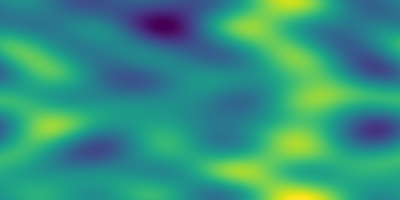
\includegraphics[interpolate=false,width=1.000000in,height=1.000000in]{burgers_rollout_lssvr_pred_0.0-img0.png}}%
\end{pgfscope}%
\begin{pgfscope}%
\pgfsetbuttcap%
\pgfsetroundjoin%
\definecolor{currentfill}{rgb}{0.000000,0.000000,0.000000}%
\pgfsetfillcolor{currentfill}%
\pgfsetlinewidth{0.803000pt}%
\definecolor{currentstroke}{rgb}{0.000000,0.000000,0.000000}%
\pgfsetstrokecolor{currentstroke}%
\pgfsetdash{}{0pt}%
\pgfsys@defobject{currentmarker}{\pgfqpoint{0.000000in}{-0.048611in}}{\pgfqpoint{0.000000in}{0.000000in}}{%
\pgfpathmoveto{\pgfqpoint{0.000000in}{0.000000in}}%
\pgfpathlineto{\pgfqpoint{0.000000in}{-0.048611in}}%
\pgfusepath{stroke,fill}%
}%
\begin{pgfscope}%
\pgfsys@transformshift{0.726837in}{0.517039in}%
\pgfsys@useobject{currentmarker}{}%
\end{pgfscope}%
\end{pgfscope}%
\begin{pgfscope}%
\definecolor{textcolor}{rgb}{0.000000,0.000000,0.000000}%
\pgfsetstrokecolor{textcolor}%
\pgfsetfillcolor{textcolor}%
\pgftext[x=0.726837in,y=0.419816in,,top]{\color{textcolor}\rmfamily\fontsize{12.000000}{14.400000}\selectfont 0}%
\end{pgfscope}%
\begin{pgfscope}%
\pgfsetbuttcap%
\pgfsetroundjoin%
\definecolor{currentfill}{rgb}{0.000000,0.000000,0.000000}%
\pgfsetfillcolor{currentfill}%
\pgfsetlinewidth{0.803000pt}%
\definecolor{currentstroke}{rgb}{0.000000,0.000000,0.000000}%
\pgfsetstrokecolor{currentstroke}%
\pgfsetdash{}{0pt}%
\pgfsys@defobject{currentmarker}{\pgfqpoint{0.000000in}{-0.048611in}}{\pgfqpoint{0.000000in}{0.000000in}}{%
\pgfpathmoveto{\pgfqpoint{0.000000in}{0.000000in}}%
\pgfpathlineto{\pgfqpoint{0.000000in}{-0.048611in}}%
\pgfusepath{stroke,fill}%
}%
\begin{pgfscope}%
\pgfsys@transformshift{1.495432in}{0.517039in}%
\pgfsys@useobject{currentmarker}{}%
\end{pgfscope}%
\end{pgfscope}%
\begin{pgfscope}%
\definecolor{textcolor}{rgb}{0.000000,0.000000,0.000000}%
\pgfsetstrokecolor{textcolor}%
\pgfsetfillcolor{textcolor}%
\pgftext[x=1.495432in,y=0.419816in,,top]{\color{textcolor}\rmfamily\fontsize{12.000000}{14.400000}\selectfont 1}%
\end{pgfscope}%
\begin{pgfscope}%
\pgfsetbuttcap%
\pgfsetroundjoin%
\definecolor{currentfill}{rgb}{0.000000,0.000000,0.000000}%
\pgfsetfillcolor{currentfill}%
\pgfsetlinewidth{0.803000pt}%
\definecolor{currentstroke}{rgb}{0.000000,0.000000,0.000000}%
\pgfsetstrokecolor{currentstroke}%
\pgfsetdash{}{0pt}%
\pgfsys@defobject{currentmarker}{\pgfqpoint{0.000000in}{-0.048611in}}{\pgfqpoint{0.000000in}{0.000000in}}{%
\pgfpathmoveto{\pgfqpoint{0.000000in}{0.000000in}}%
\pgfpathlineto{\pgfqpoint{0.000000in}{-0.048611in}}%
\pgfusepath{stroke,fill}%
}%
\begin{pgfscope}%
\pgfsys@transformshift{2.264026in}{0.517039in}%
\pgfsys@useobject{currentmarker}{}%
\end{pgfscope}%
\end{pgfscope}%
\begin{pgfscope}%
\definecolor{textcolor}{rgb}{0.000000,0.000000,0.000000}%
\pgfsetstrokecolor{textcolor}%
\pgfsetfillcolor{textcolor}%
\pgftext[x=2.264026in,y=0.419816in,,top]{\color{textcolor}\rmfamily\fontsize{12.000000}{14.400000}\selectfont 2}%
\end{pgfscope}%
\begin{pgfscope}%
\definecolor{textcolor}{rgb}{0.000000,0.000000,0.000000}%
\pgfsetstrokecolor{textcolor}%
\pgfsetfillcolor{textcolor}%
\pgftext[x=1.495432in,y=0.202965in,,top]{\color{textcolor}\rmfamily\fontsize{12.000000}{14.400000}\selectfont Space}%
\end{pgfscope}%
\begin{pgfscope}%
\pgfsetbuttcap%
\pgfsetroundjoin%
\definecolor{currentfill}{rgb}{0.000000,0.000000,0.000000}%
\pgfsetfillcolor{currentfill}%
\pgfsetlinewidth{0.803000pt}%
\definecolor{currentstroke}{rgb}{0.000000,0.000000,0.000000}%
\pgfsetstrokecolor{currentstroke}%
\pgfsetdash{}{0pt}%
\pgfsys@defobject{currentmarker}{\pgfqpoint{-0.048611in}{0.000000in}}{\pgfqpoint{-0.000000in}{0.000000in}}{%
\pgfpathmoveto{\pgfqpoint{-0.000000in}{0.000000in}}%
\pgfpathlineto{\pgfqpoint{-0.048611in}{0.000000in}}%
\pgfusepath{stroke,fill}%
}%
\begin{pgfscope}%
\pgfsys@transformshift{0.726837in}{0.517039in}%
\pgfsys@useobject{currentmarker}{}%
\end{pgfscope}%
\end{pgfscope}%
\begin{pgfscope}%
\definecolor{textcolor}{rgb}{0.000000,0.000000,0.000000}%
\pgfsetstrokecolor{textcolor}%
\pgfsetfillcolor{textcolor}%
\pgftext[x=0.364559in, y=0.453725in, left, base]{\color{textcolor}\rmfamily\fontsize{12.000000}{14.400000}\selectfont 0.0}%
\end{pgfscope}%
\begin{pgfscope}%
\pgfsetbuttcap%
\pgfsetroundjoin%
\definecolor{currentfill}{rgb}{0.000000,0.000000,0.000000}%
\pgfsetfillcolor{currentfill}%
\pgfsetlinewidth{0.803000pt}%
\definecolor{currentstroke}{rgb}{0.000000,0.000000,0.000000}%
\pgfsetstrokecolor{currentstroke}%
\pgfsetdash{}{0pt}%
\pgfsys@defobject{currentmarker}{\pgfqpoint{-0.048611in}{0.000000in}}{\pgfqpoint{-0.000000in}{0.000000in}}{%
\pgfpathmoveto{\pgfqpoint{-0.000000in}{0.000000in}}%
\pgfpathlineto{\pgfqpoint{-0.048611in}{0.000000in}}%
\pgfusepath{stroke,fill}%
}%
\begin{pgfscope}%
\pgfsys@transformshift{0.726837in}{0.861533in}%
\pgfsys@useobject{currentmarker}{}%
\end{pgfscope}%
\end{pgfscope}%
\begin{pgfscope}%
\definecolor{textcolor}{rgb}{0.000000,0.000000,0.000000}%
\pgfsetstrokecolor{textcolor}%
\pgfsetfillcolor{textcolor}%
\pgftext[x=0.364559in, y=0.798219in, left, base]{\color{textcolor}\rmfamily\fontsize{12.000000}{14.400000}\selectfont 2.5}%
\end{pgfscope}%
\begin{pgfscope}%
\pgfsetbuttcap%
\pgfsetroundjoin%
\definecolor{currentfill}{rgb}{0.000000,0.000000,0.000000}%
\pgfsetfillcolor{currentfill}%
\pgfsetlinewidth{0.803000pt}%
\definecolor{currentstroke}{rgb}{0.000000,0.000000,0.000000}%
\pgfsetstrokecolor{currentstroke}%
\pgfsetdash{}{0pt}%
\pgfsys@defobject{currentmarker}{\pgfqpoint{-0.048611in}{0.000000in}}{\pgfqpoint{-0.000000in}{0.000000in}}{%
\pgfpathmoveto{\pgfqpoint{-0.000000in}{0.000000in}}%
\pgfpathlineto{\pgfqpoint{-0.048611in}{0.000000in}}%
\pgfusepath{stroke,fill}%
}%
\begin{pgfscope}%
\pgfsys@transformshift{0.726837in}{1.206027in}%
\pgfsys@useobject{currentmarker}{}%
\end{pgfscope}%
\end{pgfscope}%
\begin{pgfscope}%
\definecolor{textcolor}{rgb}{0.000000,0.000000,0.000000}%
\pgfsetstrokecolor{textcolor}%
\pgfsetfillcolor{textcolor}%
\pgftext[x=0.364559in, y=1.142714in, left, base]{\color{textcolor}\rmfamily\fontsize{12.000000}{14.400000}\selectfont 5.0}%
\end{pgfscope}%
\begin{pgfscope}%
\pgfsetbuttcap%
\pgfsetroundjoin%
\definecolor{currentfill}{rgb}{0.000000,0.000000,0.000000}%
\pgfsetfillcolor{currentfill}%
\pgfsetlinewidth{0.803000pt}%
\definecolor{currentstroke}{rgb}{0.000000,0.000000,0.000000}%
\pgfsetstrokecolor{currentstroke}%
\pgfsetdash{}{0pt}%
\pgfsys@defobject{currentmarker}{\pgfqpoint{-0.048611in}{0.000000in}}{\pgfqpoint{-0.000000in}{0.000000in}}{%
\pgfpathmoveto{\pgfqpoint{-0.000000in}{0.000000in}}%
\pgfpathlineto{\pgfqpoint{-0.048611in}{0.000000in}}%
\pgfusepath{stroke,fill}%
}%
\begin{pgfscope}%
\pgfsys@transformshift{0.726837in}{1.550522in}%
\pgfsys@useobject{currentmarker}{}%
\end{pgfscope}%
\end{pgfscope}%
\begin{pgfscope}%
\definecolor{textcolor}{rgb}{0.000000,0.000000,0.000000}%
\pgfsetstrokecolor{textcolor}%
\pgfsetfillcolor{textcolor}%
\pgftext[x=0.364559in, y=1.487208in, left, base]{\color{textcolor}\rmfamily\fontsize{12.000000}{14.400000}\selectfont 7.5}%
\end{pgfscope}%
\begin{pgfscope}%
\pgfsetbuttcap%
\pgfsetroundjoin%
\definecolor{currentfill}{rgb}{0.000000,0.000000,0.000000}%
\pgfsetfillcolor{currentfill}%
\pgfsetlinewidth{0.803000pt}%
\definecolor{currentstroke}{rgb}{0.000000,0.000000,0.000000}%
\pgfsetstrokecolor{currentstroke}%
\pgfsetdash{}{0pt}%
\pgfsys@defobject{currentmarker}{\pgfqpoint{-0.048611in}{0.000000in}}{\pgfqpoint{-0.000000in}{0.000000in}}{%
\pgfpathmoveto{\pgfqpoint{-0.000000in}{0.000000in}}%
\pgfpathlineto{\pgfqpoint{-0.048611in}{0.000000in}}%
\pgfusepath{stroke,fill}%
}%
\begin{pgfscope}%
\pgfsys@transformshift{0.726837in}{1.895016in}%
\pgfsys@useobject{currentmarker}{}%
\end{pgfscope}%
\end{pgfscope}%
\begin{pgfscope}%
\definecolor{textcolor}{rgb}{0.000000,0.000000,0.000000}%
\pgfsetstrokecolor{textcolor}%
\pgfsetfillcolor{textcolor}%
\pgftext[x=0.258521in, y=1.831702in, left, base]{\color{textcolor}\rmfamily\fontsize{12.000000}{14.400000}\selectfont 10.0}%
\end{pgfscope}%
\begin{pgfscope}%
\definecolor{textcolor}{rgb}{0.000000,0.000000,0.000000}%
\pgfsetstrokecolor{textcolor}%
\pgfsetfillcolor{textcolor}%
\pgftext[x=0.202965in,y=1.206027in,,bottom,rotate=90.000000]{\color{textcolor}\rmfamily\fontsize{12.000000}{14.400000}\selectfont Time}%
\end{pgfscope}%
\begin{pgfscope}%
\pgfsetrectcap%
\pgfsetmiterjoin%
\pgfsetlinewidth{0.803000pt}%
\definecolor{currentstroke}{rgb}{0.000000,0.000000,0.000000}%
\pgfsetstrokecolor{currentstroke}%
\pgfsetdash{}{0pt}%
\pgfpathmoveto{\pgfqpoint{0.726837in}{0.517039in}}%
\pgfpathlineto{\pgfqpoint{0.726837in}{1.895016in}}%
\pgfusepath{stroke}%
\end{pgfscope}%
\begin{pgfscope}%
\pgfsetrectcap%
\pgfsetmiterjoin%
\pgfsetlinewidth{0.803000pt}%
\definecolor{currentstroke}{rgb}{0.000000,0.000000,0.000000}%
\pgfsetstrokecolor{currentstroke}%
\pgfsetdash{}{0pt}%
\pgfpathmoveto{\pgfqpoint{2.264026in}{0.517039in}}%
\pgfpathlineto{\pgfqpoint{2.264026in}{1.895016in}}%
\pgfusepath{stroke}%
\end{pgfscope}%
\begin{pgfscope}%
\pgfsetrectcap%
\pgfsetmiterjoin%
\pgfsetlinewidth{0.803000pt}%
\definecolor{currentstroke}{rgb}{0.000000,0.000000,0.000000}%
\pgfsetstrokecolor{currentstroke}%
\pgfsetdash{}{0pt}%
\pgfpathmoveto{\pgfqpoint{0.726837in}{0.517039in}}%
\pgfpathlineto{\pgfqpoint{2.264026in}{0.517039in}}%
\pgfusepath{stroke}%
\end{pgfscope}%
\begin{pgfscope}%
\pgfsetrectcap%
\pgfsetmiterjoin%
\pgfsetlinewidth{0.803000pt}%
\definecolor{currentstroke}{rgb}{0.000000,0.000000,0.000000}%
\pgfsetstrokecolor{currentstroke}%
\pgfsetdash{}{0pt}%
\pgfpathmoveto{\pgfqpoint{0.726837in}{1.895016in}}%
\pgfpathlineto{\pgfqpoint{2.264026in}{1.895016in}}%
\pgfusepath{stroke}%
\end{pgfscope}%
\begin{pgfscope}%
\pgfsetbuttcap%
\pgfsetmiterjoin%
\pgfsetlinewidth{0.000000pt}%
\definecolor{currentstroke}{rgb}{0.000000,0.000000,0.000000}%
\pgfsetstrokecolor{currentstroke}%
\pgfsetstrokeopacity{0.000000}%
\pgfsetdash{}{0pt}%
\pgfpathmoveto{\pgfqpoint{2.393905in}{0.517039in}}%
\pgfpathlineto{\pgfqpoint{2.462804in}{0.517039in}}%
\pgfpathlineto{\pgfqpoint{2.462804in}{1.895016in}}%
\pgfpathlineto{\pgfqpoint{2.393905in}{1.895016in}}%
\pgfpathlineto{\pgfqpoint{2.393905in}{0.517039in}}%
\pgfpathclose%
\pgfusepath{}%
\end{pgfscope}%
\begin{pgfscope}%
\pgfsys@transformshift{2.390000in}{0.520000in}%
\pgftext[left,bottom]{
\includegraphics[interpolate=true,width=0.070000in,height=1.380000in]{burgers_rollout_lssvr_pred_0.0-img1.png}}%
\end{pgfscope}%
\begin{pgfscope}%
\pgfsetbuttcap%
\pgfsetroundjoin%
\definecolor{currentfill}{rgb}{0.000000,0.000000,0.000000}%
\pgfsetfillcolor{currentfill}%
\pgfsetlinewidth{0.803000pt}%
\definecolor{currentstroke}{rgb}{0.000000,0.000000,0.000000}%
\pgfsetstrokecolor{currentstroke}%
\pgfsetdash{}{0pt}%
\pgfsys@defobject{currentmarker}{\pgfqpoint{0.000000in}{0.000000in}}{\pgfqpoint{0.048611in}{0.000000in}}{%
\pgfpathmoveto{\pgfqpoint{0.000000in}{0.000000in}}%
\pgfpathlineto{\pgfqpoint{0.048611in}{0.000000in}}%
\pgfusepath{stroke,fill}%
}%
\begin{pgfscope}%
\pgfsys@transformshift{2.462804in}{0.839076in}%
\pgfsys@useobject{currentmarker}{}%
\end{pgfscope}%
\end{pgfscope}%
\begin{pgfscope}%
\definecolor{textcolor}{rgb}{0.000000,0.000000,0.000000}%
\pgfsetstrokecolor{textcolor}%
\pgfsetfillcolor{textcolor}%
\pgftext[x=2.560026in, y=0.775762in, left, base]{\color{textcolor}\rmfamily\fontsize{12.000000}{14.400000}\selectfont \ensuremath{-}0.5}%
\end{pgfscope}%
\begin{pgfscope}%
\pgfsetbuttcap%
\pgfsetroundjoin%
\definecolor{currentfill}{rgb}{0.000000,0.000000,0.000000}%
\pgfsetfillcolor{currentfill}%
\pgfsetlinewidth{0.803000pt}%
\definecolor{currentstroke}{rgb}{0.000000,0.000000,0.000000}%
\pgfsetstrokecolor{currentstroke}%
\pgfsetdash{}{0pt}%
\pgfsys@defobject{currentmarker}{\pgfqpoint{0.000000in}{0.000000in}}{\pgfqpoint{0.048611in}{0.000000in}}{%
\pgfpathmoveto{\pgfqpoint{0.000000in}{0.000000in}}%
\pgfpathlineto{\pgfqpoint{0.048611in}{0.000000in}}%
\pgfusepath{stroke,fill}%
}%
\begin{pgfscope}%
\pgfsys@transformshift{2.462804in}{1.206027in}%
\pgfsys@useobject{currentmarker}{}%
\end{pgfscope}%
\end{pgfscope}%
\begin{pgfscope}%
\definecolor{textcolor}{rgb}{0.000000,0.000000,0.000000}%
\pgfsetstrokecolor{textcolor}%
\pgfsetfillcolor{textcolor}%
\pgftext[x=2.560026in, y=1.142714in, left, base]{\color{textcolor}\rmfamily\fontsize{12.000000}{14.400000}\selectfont 0.0}%
\end{pgfscope}%
\begin{pgfscope}%
\pgfsetbuttcap%
\pgfsetroundjoin%
\definecolor{currentfill}{rgb}{0.000000,0.000000,0.000000}%
\pgfsetfillcolor{currentfill}%
\pgfsetlinewidth{0.803000pt}%
\definecolor{currentstroke}{rgb}{0.000000,0.000000,0.000000}%
\pgfsetstrokecolor{currentstroke}%
\pgfsetdash{}{0pt}%
\pgfsys@defobject{currentmarker}{\pgfqpoint{0.000000in}{0.000000in}}{\pgfqpoint{0.048611in}{0.000000in}}{%
\pgfpathmoveto{\pgfqpoint{0.000000in}{0.000000in}}%
\pgfpathlineto{\pgfqpoint{0.048611in}{0.000000in}}%
\pgfusepath{stroke,fill}%
}%
\begin{pgfscope}%
\pgfsys@transformshift{2.462804in}{1.572979in}%
\pgfsys@useobject{currentmarker}{}%
\end{pgfscope}%
\end{pgfscope}%
\begin{pgfscope}%
\definecolor{textcolor}{rgb}{0.000000,0.000000,0.000000}%
\pgfsetstrokecolor{textcolor}%
\pgfsetfillcolor{textcolor}%
\pgftext[x=2.560026in, y=1.509665in, left, base]{\color{textcolor}\rmfamily\fontsize{12.000000}{14.400000}\selectfont 0.5}%
\end{pgfscope}%
\begin{pgfscope}%
\pgfsetrectcap%
\pgfsetmiterjoin%
\pgfsetlinewidth{0.803000pt}%
\definecolor{currentstroke}{rgb}{0.000000,0.000000,0.000000}%
\pgfsetstrokecolor{currentstroke}%
\pgfsetdash{}{0pt}%
\pgfpathmoveto{\pgfqpoint{2.393905in}{0.517039in}}%
\pgfpathlineto{\pgfqpoint{2.428354in}{0.517039in}}%
\pgfpathlineto{\pgfqpoint{2.462804in}{0.517039in}}%
\pgfpathlineto{\pgfqpoint{2.462804in}{1.895016in}}%
\pgfpathlineto{\pgfqpoint{2.428354in}{1.895016in}}%
\pgfpathlineto{\pgfqpoint{2.393905in}{1.895016in}}%
\pgfpathlineto{\pgfqpoint{2.393905in}{0.517039in}}%
\pgfpathclose%
\pgfusepath{stroke}%
\end{pgfscope}%
\end{pgfpicture}%
\makeatother%
\endgroup%

      \end{adjustbox}
      \caption{SpectralSVR prediction.}\label{fig:comp_lssvr_pred_0.0}
    \end{subfigure}
    \begin{subfigure}{0.49\linewidth}
      \begin{adjustbox}{width=\linewidth}
        \begingroup%
\makeatletter%
\begin{pgfpicture}%
\pgfpathrectangle{\pgfpointorigin}{\pgfqpoint{3.000000in}{2.000000in}}%
\pgfusepath{use as bounding box, clip}%
\begin{pgfscope}%
\pgfsetbuttcap%
\pgfsetmiterjoin%
\pgfsetlinewidth{0.000000pt}%
\definecolor{currentstroke}{rgb}{0.000000,0.000000,0.000000}%
\pgfsetstrokecolor{currentstroke}%
\pgfsetstrokeopacity{0.000000}%
\pgfsetdash{}{0pt}%
\pgfpathmoveto{\pgfqpoint{0.000000in}{0.000000in}}%
\pgfpathlineto{\pgfqpoint{3.000000in}{0.000000in}}%
\pgfpathlineto{\pgfqpoint{3.000000in}{2.000000in}}%
\pgfpathlineto{\pgfqpoint{0.000000in}{2.000000in}}%
\pgfpathlineto{\pgfqpoint{0.000000in}{0.000000in}}%
\pgfpathclose%
\pgfusepath{}%
\end{pgfscope}%
\begin{pgfscope}%
\pgfsetbuttcap%
\pgfsetmiterjoin%
\pgfsetlinewidth{0.000000pt}%
\definecolor{currentstroke}{rgb}{0.000000,0.000000,0.000000}%
\pgfsetstrokecolor{currentstroke}%
\pgfsetstrokeopacity{0.000000}%
\pgfsetdash{}{0pt}%
\pgfpathmoveto{\pgfqpoint{0.726837in}{0.517039in}}%
\pgfpathlineto{\pgfqpoint{2.264026in}{0.517039in}}%
\pgfpathlineto{\pgfqpoint{2.264026in}{1.895016in}}%
\pgfpathlineto{\pgfqpoint{0.726837in}{1.895016in}}%
\pgfpathlineto{\pgfqpoint{0.726837in}{0.517039in}}%
\pgfpathclose%
\pgfusepath{}%
\end{pgfscope}%
\begin{pgfscope}%
\pgfpathrectangle{\pgfqpoint{0.726837in}{0.517039in}}{\pgfqpoint{1.537189in}{1.377978in}}%
\pgfusepath{clip}%
\pgfsys@transformcm{1.537189}{0.000000}{0.000000}{1.377978}{0.726837in}{0.517039in}%
\pgftext[left,bottom]{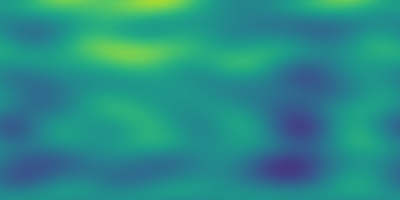
\includegraphics[interpolate=false,width=1.000000in,height=1.000000in]{burgers_rollout_lssvr_diff_0.0-img0.png}}%
\end{pgfscope}%
\begin{pgfscope}%
\pgfsetbuttcap%
\pgfsetroundjoin%
\definecolor{currentfill}{rgb}{0.000000,0.000000,0.000000}%
\pgfsetfillcolor{currentfill}%
\pgfsetlinewidth{0.803000pt}%
\definecolor{currentstroke}{rgb}{0.000000,0.000000,0.000000}%
\pgfsetstrokecolor{currentstroke}%
\pgfsetdash{}{0pt}%
\pgfsys@defobject{currentmarker}{\pgfqpoint{0.000000in}{-0.048611in}}{\pgfqpoint{0.000000in}{0.000000in}}{%
\pgfpathmoveto{\pgfqpoint{0.000000in}{0.000000in}}%
\pgfpathlineto{\pgfqpoint{0.000000in}{-0.048611in}}%
\pgfusepath{stroke,fill}%
}%
\begin{pgfscope}%
\pgfsys@transformshift{0.726837in}{0.517039in}%
\pgfsys@useobject{currentmarker}{}%
\end{pgfscope}%
\end{pgfscope}%
\begin{pgfscope}%
\definecolor{textcolor}{rgb}{0.000000,0.000000,0.000000}%
\pgfsetstrokecolor{textcolor}%
\pgfsetfillcolor{textcolor}%
\pgftext[x=0.726837in,y=0.419816in,,top]{\color{textcolor}\rmfamily\fontsize{12.000000}{14.400000}\selectfont 0}%
\end{pgfscope}%
\begin{pgfscope}%
\pgfsetbuttcap%
\pgfsetroundjoin%
\definecolor{currentfill}{rgb}{0.000000,0.000000,0.000000}%
\pgfsetfillcolor{currentfill}%
\pgfsetlinewidth{0.803000pt}%
\definecolor{currentstroke}{rgb}{0.000000,0.000000,0.000000}%
\pgfsetstrokecolor{currentstroke}%
\pgfsetdash{}{0pt}%
\pgfsys@defobject{currentmarker}{\pgfqpoint{0.000000in}{-0.048611in}}{\pgfqpoint{0.000000in}{0.000000in}}{%
\pgfpathmoveto{\pgfqpoint{0.000000in}{0.000000in}}%
\pgfpathlineto{\pgfqpoint{0.000000in}{-0.048611in}}%
\pgfusepath{stroke,fill}%
}%
\begin{pgfscope}%
\pgfsys@transformshift{1.495432in}{0.517039in}%
\pgfsys@useobject{currentmarker}{}%
\end{pgfscope}%
\end{pgfscope}%
\begin{pgfscope}%
\definecolor{textcolor}{rgb}{0.000000,0.000000,0.000000}%
\pgfsetstrokecolor{textcolor}%
\pgfsetfillcolor{textcolor}%
\pgftext[x=1.495432in,y=0.419816in,,top]{\color{textcolor}\rmfamily\fontsize{12.000000}{14.400000}\selectfont 1}%
\end{pgfscope}%
\begin{pgfscope}%
\pgfsetbuttcap%
\pgfsetroundjoin%
\definecolor{currentfill}{rgb}{0.000000,0.000000,0.000000}%
\pgfsetfillcolor{currentfill}%
\pgfsetlinewidth{0.803000pt}%
\definecolor{currentstroke}{rgb}{0.000000,0.000000,0.000000}%
\pgfsetstrokecolor{currentstroke}%
\pgfsetdash{}{0pt}%
\pgfsys@defobject{currentmarker}{\pgfqpoint{0.000000in}{-0.048611in}}{\pgfqpoint{0.000000in}{0.000000in}}{%
\pgfpathmoveto{\pgfqpoint{0.000000in}{0.000000in}}%
\pgfpathlineto{\pgfqpoint{0.000000in}{-0.048611in}}%
\pgfusepath{stroke,fill}%
}%
\begin{pgfscope}%
\pgfsys@transformshift{2.264026in}{0.517039in}%
\pgfsys@useobject{currentmarker}{}%
\end{pgfscope}%
\end{pgfscope}%
\begin{pgfscope}%
\definecolor{textcolor}{rgb}{0.000000,0.000000,0.000000}%
\pgfsetstrokecolor{textcolor}%
\pgfsetfillcolor{textcolor}%
\pgftext[x=2.264026in,y=0.419816in,,top]{\color{textcolor}\rmfamily\fontsize{12.000000}{14.400000}\selectfont 2}%
\end{pgfscope}%
\begin{pgfscope}%
\definecolor{textcolor}{rgb}{0.000000,0.000000,0.000000}%
\pgfsetstrokecolor{textcolor}%
\pgfsetfillcolor{textcolor}%
\pgftext[x=1.495432in,y=0.202965in,,top]{\color{textcolor}\rmfamily\fontsize{12.000000}{14.400000}\selectfont Space}%
\end{pgfscope}%
\begin{pgfscope}%
\pgfsetbuttcap%
\pgfsetroundjoin%
\definecolor{currentfill}{rgb}{0.000000,0.000000,0.000000}%
\pgfsetfillcolor{currentfill}%
\pgfsetlinewidth{0.803000pt}%
\definecolor{currentstroke}{rgb}{0.000000,0.000000,0.000000}%
\pgfsetstrokecolor{currentstroke}%
\pgfsetdash{}{0pt}%
\pgfsys@defobject{currentmarker}{\pgfqpoint{-0.048611in}{0.000000in}}{\pgfqpoint{-0.000000in}{0.000000in}}{%
\pgfpathmoveto{\pgfqpoint{-0.000000in}{0.000000in}}%
\pgfpathlineto{\pgfqpoint{-0.048611in}{0.000000in}}%
\pgfusepath{stroke,fill}%
}%
\begin{pgfscope}%
\pgfsys@transformshift{0.726837in}{0.517039in}%
\pgfsys@useobject{currentmarker}{}%
\end{pgfscope}%
\end{pgfscope}%
\begin{pgfscope}%
\definecolor{textcolor}{rgb}{0.000000,0.000000,0.000000}%
\pgfsetstrokecolor{textcolor}%
\pgfsetfillcolor{textcolor}%
\pgftext[x=0.364559in, y=0.453725in, left, base]{\color{textcolor}\rmfamily\fontsize{12.000000}{14.400000}\selectfont 0.0}%
\end{pgfscope}%
\begin{pgfscope}%
\pgfsetbuttcap%
\pgfsetroundjoin%
\definecolor{currentfill}{rgb}{0.000000,0.000000,0.000000}%
\pgfsetfillcolor{currentfill}%
\pgfsetlinewidth{0.803000pt}%
\definecolor{currentstroke}{rgb}{0.000000,0.000000,0.000000}%
\pgfsetstrokecolor{currentstroke}%
\pgfsetdash{}{0pt}%
\pgfsys@defobject{currentmarker}{\pgfqpoint{-0.048611in}{0.000000in}}{\pgfqpoint{-0.000000in}{0.000000in}}{%
\pgfpathmoveto{\pgfqpoint{-0.000000in}{0.000000in}}%
\pgfpathlineto{\pgfqpoint{-0.048611in}{0.000000in}}%
\pgfusepath{stroke,fill}%
}%
\begin{pgfscope}%
\pgfsys@transformshift{0.726837in}{0.861533in}%
\pgfsys@useobject{currentmarker}{}%
\end{pgfscope}%
\end{pgfscope}%
\begin{pgfscope}%
\definecolor{textcolor}{rgb}{0.000000,0.000000,0.000000}%
\pgfsetstrokecolor{textcolor}%
\pgfsetfillcolor{textcolor}%
\pgftext[x=0.364559in, y=0.798219in, left, base]{\color{textcolor}\rmfamily\fontsize{12.000000}{14.400000}\selectfont 2.5}%
\end{pgfscope}%
\begin{pgfscope}%
\pgfsetbuttcap%
\pgfsetroundjoin%
\definecolor{currentfill}{rgb}{0.000000,0.000000,0.000000}%
\pgfsetfillcolor{currentfill}%
\pgfsetlinewidth{0.803000pt}%
\definecolor{currentstroke}{rgb}{0.000000,0.000000,0.000000}%
\pgfsetstrokecolor{currentstroke}%
\pgfsetdash{}{0pt}%
\pgfsys@defobject{currentmarker}{\pgfqpoint{-0.048611in}{0.000000in}}{\pgfqpoint{-0.000000in}{0.000000in}}{%
\pgfpathmoveto{\pgfqpoint{-0.000000in}{0.000000in}}%
\pgfpathlineto{\pgfqpoint{-0.048611in}{0.000000in}}%
\pgfusepath{stroke,fill}%
}%
\begin{pgfscope}%
\pgfsys@transformshift{0.726837in}{1.206027in}%
\pgfsys@useobject{currentmarker}{}%
\end{pgfscope}%
\end{pgfscope}%
\begin{pgfscope}%
\definecolor{textcolor}{rgb}{0.000000,0.000000,0.000000}%
\pgfsetstrokecolor{textcolor}%
\pgfsetfillcolor{textcolor}%
\pgftext[x=0.364559in, y=1.142714in, left, base]{\color{textcolor}\rmfamily\fontsize{12.000000}{14.400000}\selectfont 5.0}%
\end{pgfscope}%
\begin{pgfscope}%
\pgfsetbuttcap%
\pgfsetroundjoin%
\definecolor{currentfill}{rgb}{0.000000,0.000000,0.000000}%
\pgfsetfillcolor{currentfill}%
\pgfsetlinewidth{0.803000pt}%
\definecolor{currentstroke}{rgb}{0.000000,0.000000,0.000000}%
\pgfsetstrokecolor{currentstroke}%
\pgfsetdash{}{0pt}%
\pgfsys@defobject{currentmarker}{\pgfqpoint{-0.048611in}{0.000000in}}{\pgfqpoint{-0.000000in}{0.000000in}}{%
\pgfpathmoveto{\pgfqpoint{-0.000000in}{0.000000in}}%
\pgfpathlineto{\pgfqpoint{-0.048611in}{0.000000in}}%
\pgfusepath{stroke,fill}%
}%
\begin{pgfscope}%
\pgfsys@transformshift{0.726837in}{1.550522in}%
\pgfsys@useobject{currentmarker}{}%
\end{pgfscope}%
\end{pgfscope}%
\begin{pgfscope}%
\definecolor{textcolor}{rgb}{0.000000,0.000000,0.000000}%
\pgfsetstrokecolor{textcolor}%
\pgfsetfillcolor{textcolor}%
\pgftext[x=0.364559in, y=1.487208in, left, base]{\color{textcolor}\rmfamily\fontsize{12.000000}{14.400000}\selectfont 7.5}%
\end{pgfscope}%
\begin{pgfscope}%
\pgfsetbuttcap%
\pgfsetroundjoin%
\definecolor{currentfill}{rgb}{0.000000,0.000000,0.000000}%
\pgfsetfillcolor{currentfill}%
\pgfsetlinewidth{0.803000pt}%
\definecolor{currentstroke}{rgb}{0.000000,0.000000,0.000000}%
\pgfsetstrokecolor{currentstroke}%
\pgfsetdash{}{0pt}%
\pgfsys@defobject{currentmarker}{\pgfqpoint{-0.048611in}{0.000000in}}{\pgfqpoint{-0.000000in}{0.000000in}}{%
\pgfpathmoveto{\pgfqpoint{-0.000000in}{0.000000in}}%
\pgfpathlineto{\pgfqpoint{-0.048611in}{0.000000in}}%
\pgfusepath{stroke,fill}%
}%
\begin{pgfscope}%
\pgfsys@transformshift{0.726837in}{1.895016in}%
\pgfsys@useobject{currentmarker}{}%
\end{pgfscope}%
\end{pgfscope}%
\begin{pgfscope}%
\definecolor{textcolor}{rgb}{0.000000,0.000000,0.000000}%
\pgfsetstrokecolor{textcolor}%
\pgfsetfillcolor{textcolor}%
\pgftext[x=0.258521in, y=1.831702in, left, base]{\color{textcolor}\rmfamily\fontsize{12.000000}{14.400000}\selectfont 10.0}%
\end{pgfscope}%
\begin{pgfscope}%
\definecolor{textcolor}{rgb}{0.000000,0.000000,0.000000}%
\pgfsetstrokecolor{textcolor}%
\pgfsetfillcolor{textcolor}%
\pgftext[x=0.202965in,y=1.206027in,,bottom,rotate=90.000000]{\color{textcolor}\rmfamily\fontsize{12.000000}{14.400000}\selectfont Time}%
\end{pgfscope}%
\begin{pgfscope}%
\pgfsetrectcap%
\pgfsetmiterjoin%
\pgfsetlinewidth{0.803000pt}%
\definecolor{currentstroke}{rgb}{0.000000,0.000000,0.000000}%
\pgfsetstrokecolor{currentstroke}%
\pgfsetdash{}{0pt}%
\pgfpathmoveto{\pgfqpoint{0.726837in}{0.517039in}}%
\pgfpathlineto{\pgfqpoint{0.726837in}{1.895016in}}%
\pgfusepath{stroke}%
\end{pgfscope}%
\begin{pgfscope}%
\pgfsetrectcap%
\pgfsetmiterjoin%
\pgfsetlinewidth{0.803000pt}%
\definecolor{currentstroke}{rgb}{0.000000,0.000000,0.000000}%
\pgfsetstrokecolor{currentstroke}%
\pgfsetdash{}{0pt}%
\pgfpathmoveto{\pgfqpoint{2.264026in}{0.517039in}}%
\pgfpathlineto{\pgfqpoint{2.264026in}{1.895016in}}%
\pgfusepath{stroke}%
\end{pgfscope}%
\begin{pgfscope}%
\pgfsetrectcap%
\pgfsetmiterjoin%
\pgfsetlinewidth{0.803000pt}%
\definecolor{currentstroke}{rgb}{0.000000,0.000000,0.000000}%
\pgfsetstrokecolor{currentstroke}%
\pgfsetdash{}{0pt}%
\pgfpathmoveto{\pgfqpoint{0.726837in}{0.517039in}}%
\pgfpathlineto{\pgfqpoint{2.264026in}{0.517039in}}%
\pgfusepath{stroke}%
\end{pgfscope}%
\begin{pgfscope}%
\pgfsetrectcap%
\pgfsetmiterjoin%
\pgfsetlinewidth{0.803000pt}%
\definecolor{currentstroke}{rgb}{0.000000,0.000000,0.000000}%
\pgfsetstrokecolor{currentstroke}%
\pgfsetdash{}{0pt}%
\pgfpathmoveto{\pgfqpoint{0.726837in}{1.895016in}}%
\pgfpathlineto{\pgfqpoint{2.264026in}{1.895016in}}%
\pgfusepath{stroke}%
\end{pgfscope}%
\begin{pgfscope}%
\pgfsetbuttcap%
\pgfsetmiterjoin%
\pgfsetlinewidth{0.000000pt}%
\definecolor{currentstroke}{rgb}{0.000000,0.000000,0.000000}%
\pgfsetstrokecolor{currentstroke}%
\pgfsetstrokeopacity{0.000000}%
\pgfsetdash{}{0pt}%
\pgfpathmoveto{\pgfqpoint{2.393905in}{0.517039in}}%
\pgfpathlineto{\pgfqpoint{2.462804in}{0.517039in}}%
\pgfpathlineto{\pgfqpoint{2.462804in}{1.895016in}}%
\pgfpathlineto{\pgfqpoint{2.393905in}{1.895016in}}%
\pgfpathlineto{\pgfqpoint{2.393905in}{0.517039in}}%
\pgfpathclose%
\pgfusepath{}%
\end{pgfscope}%
\begin{pgfscope}%
\pgfsys@transformshift{2.390000in}{0.520000in}%
\pgftext[left,bottom]{
\includegraphics[interpolate=true,width=0.070000in,height=1.380000in]{burgers_rollout_lssvr_diff_0.0-img1.png}}%
\end{pgfscope}%
\begin{pgfscope}%
\pgfsetbuttcap%
\pgfsetroundjoin%
\definecolor{currentfill}{rgb}{0.000000,0.000000,0.000000}%
\pgfsetfillcolor{currentfill}%
\pgfsetlinewidth{0.803000pt}%
\definecolor{currentstroke}{rgb}{0.000000,0.000000,0.000000}%
\pgfsetstrokecolor{currentstroke}%
\pgfsetdash{}{0pt}%
\pgfsys@defobject{currentmarker}{\pgfqpoint{0.000000in}{0.000000in}}{\pgfqpoint{0.048611in}{0.000000in}}{%
\pgfpathmoveto{\pgfqpoint{0.000000in}{0.000000in}}%
\pgfpathlineto{\pgfqpoint{0.048611in}{0.000000in}}%
\pgfusepath{stroke,fill}%
}%
\begin{pgfscope}%
\pgfsys@transformshift{2.462804in}{0.839076in}%
\pgfsys@useobject{currentmarker}{}%
\end{pgfscope}%
\end{pgfscope}%
\begin{pgfscope}%
\definecolor{textcolor}{rgb}{0.000000,0.000000,0.000000}%
\pgfsetstrokecolor{textcolor}%
\pgfsetfillcolor{textcolor}%
\pgftext[x=2.560026in, y=0.775762in, left, base]{\color{textcolor}\rmfamily\fontsize{12.000000}{14.400000}\selectfont \ensuremath{-}0.5}%
\end{pgfscope}%
\begin{pgfscope}%
\pgfsetbuttcap%
\pgfsetroundjoin%
\definecolor{currentfill}{rgb}{0.000000,0.000000,0.000000}%
\pgfsetfillcolor{currentfill}%
\pgfsetlinewidth{0.803000pt}%
\definecolor{currentstroke}{rgb}{0.000000,0.000000,0.000000}%
\pgfsetstrokecolor{currentstroke}%
\pgfsetdash{}{0pt}%
\pgfsys@defobject{currentmarker}{\pgfqpoint{0.000000in}{0.000000in}}{\pgfqpoint{0.048611in}{0.000000in}}{%
\pgfpathmoveto{\pgfqpoint{0.000000in}{0.000000in}}%
\pgfpathlineto{\pgfqpoint{0.048611in}{0.000000in}}%
\pgfusepath{stroke,fill}%
}%
\begin{pgfscope}%
\pgfsys@transformshift{2.462804in}{1.206027in}%
\pgfsys@useobject{currentmarker}{}%
\end{pgfscope}%
\end{pgfscope}%
\begin{pgfscope}%
\definecolor{textcolor}{rgb}{0.000000,0.000000,0.000000}%
\pgfsetstrokecolor{textcolor}%
\pgfsetfillcolor{textcolor}%
\pgftext[x=2.560026in, y=1.142714in, left, base]{\color{textcolor}\rmfamily\fontsize{12.000000}{14.400000}\selectfont 0.0}%
\end{pgfscope}%
\begin{pgfscope}%
\pgfsetbuttcap%
\pgfsetroundjoin%
\definecolor{currentfill}{rgb}{0.000000,0.000000,0.000000}%
\pgfsetfillcolor{currentfill}%
\pgfsetlinewidth{0.803000pt}%
\definecolor{currentstroke}{rgb}{0.000000,0.000000,0.000000}%
\pgfsetstrokecolor{currentstroke}%
\pgfsetdash{}{0pt}%
\pgfsys@defobject{currentmarker}{\pgfqpoint{0.000000in}{0.000000in}}{\pgfqpoint{0.048611in}{0.000000in}}{%
\pgfpathmoveto{\pgfqpoint{0.000000in}{0.000000in}}%
\pgfpathlineto{\pgfqpoint{0.048611in}{0.000000in}}%
\pgfusepath{stroke,fill}%
}%
\begin{pgfscope}%
\pgfsys@transformshift{2.462804in}{1.572979in}%
\pgfsys@useobject{currentmarker}{}%
\end{pgfscope}%
\end{pgfscope}%
\begin{pgfscope}%
\definecolor{textcolor}{rgb}{0.000000,0.000000,0.000000}%
\pgfsetstrokecolor{textcolor}%
\pgfsetfillcolor{textcolor}%
\pgftext[x=2.560026in, y=1.509665in, left, base]{\color{textcolor}\rmfamily\fontsize{12.000000}{14.400000}\selectfont 0.5}%
\end{pgfscope}%
\begin{pgfscope}%
\pgfsetrectcap%
\pgfsetmiterjoin%
\pgfsetlinewidth{0.803000pt}%
\definecolor{currentstroke}{rgb}{0.000000,0.000000,0.000000}%
\pgfsetstrokecolor{currentstroke}%
\pgfsetdash{}{0pt}%
\pgfpathmoveto{\pgfqpoint{2.393905in}{0.517039in}}%
\pgfpathlineto{\pgfqpoint{2.428354in}{0.517039in}}%
\pgfpathlineto{\pgfqpoint{2.462804in}{0.517039in}}%
\pgfpathlineto{\pgfqpoint{2.462804in}{1.895016in}}%
\pgfpathlineto{\pgfqpoint{2.428354in}{1.895016in}}%
\pgfpathlineto{\pgfqpoint{2.393905in}{1.895016in}}%
\pgfpathlineto{\pgfqpoint{2.393905in}{0.517039in}}%
\pgfpathclose%
\pgfusepath{stroke}%
\end{pgfscope}%
\end{pgfpicture}%
\makeatother%
\endgroup%

      \end{adjustbox}
      \caption{SpectralSVR difference with target.}\label{fig:comp_lssvr_diff_0.0}
    \end{subfigure}
    \begin{subfigure}{0.49\linewidth}
      \begin{adjustbox}{width=\linewidth}
        \begingroup%
\makeatletter%
\begin{pgfpicture}%
\pgfpathrectangle{\pgfpointorigin}{\pgfqpoint{3.000000in}{2.000000in}}%
\pgfusepath{use as bounding box, clip}%
\begin{pgfscope}%
\pgfsetbuttcap%
\pgfsetmiterjoin%
\pgfsetlinewidth{0.000000pt}%
\definecolor{currentstroke}{rgb}{0.000000,0.000000,0.000000}%
\pgfsetstrokecolor{currentstroke}%
\pgfsetstrokeopacity{0.000000}%
\pgfsetdash{}{0pt}%
\pgfpathmoveto{\pgfqpoint{0.000000in}{0.000000in}}%
\pgfpathlineto{\pgfqpoint{3.000000in}{0.000000in}}%
\pgfpathlineto{\pgfqpoint{3.000000in}{2.000000in}}%
\pgfpathlineto{\pgfqpoint{0.000000in}{2.000000in}}%
\pgfpathlineto{\pgfqpoint{0.000000in}{0.000000in}}%
\pgfpathclose%
\pgfusepath{}%
\end{pgfscope}%
\begin{pgfscope}%
\pgfsetbuttcap%
\pgfsetmiterjoin%
\pgfsetlinewidth{0.000000pt}%
\definecolor{currentstroke}{rgb}{0.000000,0.000000,0.000000}%
\pgfsetstrokecolor{currentstroke}%
\pgfsetstrokeopacity{0.000000}%
\pgfsetdash{}{0pt}%
\pgfpathmoveto{\pgfqpoint{0.726837in}{0.517039in}}%
\pgfpathlineto{\pgfqpoint{2.264026in}{0.517039in}}%
\pgfpathlineto{\pgfqpoint{2.264026in}{1.895016in}}%
\pgfpathlineto{\pgfqpoint{0.726837in}{1.895016in}}%
\pgfpathlineto{\pgfqpoint{0.726837in}{0.517039in}}%
\pgfpathclose%
\pgfusepath{}%
\end{pgfscope}%
\begin{pgfscope}%
\pgfpathrectangle{\pgfqpoint{0.726837in}{0.517039in}}{\pgfqpoint{1.537189in}{1.377978in}}%
\pgfusepath{clip}%
\pgfsys@transformcm{1.537189}{0.000000}{0.000000}{1.377978}{0.726837in}{0.517039in}%
\pgftext[left,bottom]{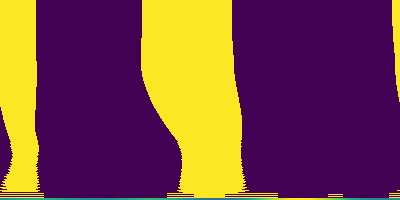
\includegraphics[interpolate=false,width=1.000000in,height=1.000000in]{burgers_rollout_fnn_pred_0.0-img0.png}}%
\end{pgfscope}%
\begin{pgfscope}%
\pgfsetbuttcap%
\pgfsetroundjoin%
\definecolor{currentfill}{rgb}{0.000000,0.000000,0.000000}%
\pgfsetfillcolor{currentfill}%
\pgfsetlinewidth{0.803000pt}%
\definecolor{currentstroke}{rgb}{0.000000,0.000000,0.000000}%
\pgfsetstrokecolor{currentstroke}%
\pgfsetdash{}{0pt}%
\pgfsys@defobject{currentmarker}{\pgfqpoint{0.000000in}{-0.048611in}}{\pgfqpoint{0.000000in}{0.000000in}}{%
\pgfpathmoveto{\pgfqpoint{0.000000in}{0.000000in}}%
\pgfpathlineto{\pgfqpoint{0.000000in}{-0.048611in}}%
\pgfusepath{stroke,fill}%
}%
\begin{pgfscope}%
\pgfsys@transformshift{0.726837in}{0.517039in}%
\pgfsys@useobject{currentmarker}{}%
\end{pgfscope}%
\end{pgfscope}%
\begin{pgfscope}%
\definecolor{textcolor}{rgb}{0.000000,0.000000,0.000000}%
\pgfsetstrokecolor{textcolor}%
\pgfsetfillcolor{textcolor}%
\pgftext[x=0.726837in,y=0.419816in,,top]{\color{textcolor}\rmfamily\fontsize{12.000000}{14.400000}\selectfont 0}%
\end{pgfscope}%
\begin{pgfscope}%
\pgfsetbuttcap%
\pgfsetroundjoin%
\definecolor{currentfill}{rgb}{0.000000,0.000000,0.000000}%
\pgfsetfillcolor{currentfill}%
\pgfsetlinewidth{0.803000pt}%
\definecolor{currentstroke}{rgb}{0.000000,0.000000,0.000000}%
\pgfsetstrokecolor{currentstroke}%
\pgfsetdash{}{0pt}%
\pgfsys@defobject{currentmarker}{\pgfqpoint{0.000000in}{-0.048611in}}{\pgfqpoint{0.000000in}{0.000000in}}{%
\pgfpathmoveto{\pgfqpoint{0.000000in}{0.000000in}}%
\pgfpathlineto{\pgfqpoint{0.000000in}{-0.048611in}}%
\pgfusepath{stroke,fill}%
}%
\begin{pgfscope}%
\pgfsys@transformshift{1.495432in}{0.517039in}%
\pgfsys@useobject{currentmarker}{}%
\end{pgfscope}%
\end{pgfscope}%
\begin{pgfscope}%
\definecolor{textcolor}{rgb}{0.000000,0.000000,0.000000}%
\pgfsetstrokecolor{textcolor}%
\pgfsetfillcolor{textcolor}%
\pgftext[x=1.495432in,y=0.419816in,,top]{\color{textcolor}\rmfamily\fontsize{12.000000}{14.400000}\selectfont 1}%
\end{pgfscope}%
\begin{pgfscope}%
\pgfsetbuttcap%
\pgfsetroundjoin%
\definecolor{currentfill}{rgb}{0.000000,0.000000,0.000000}%
\pgfsetfillcolor{currentfill}%
\pgfsetlinewidth{0.803000pt}%
\definecolor{currentstroke}{rgb}{0.000000,0.000000,0.000000}%
\pgfsetstrokecolor{currentstroke}%
\pgfsetdash{}{0pt}%
\pgfsys@defobject{currentmarker}{\pgfqpoint{0.000000in}{-0.048611in}}{\pgfqpoint{0.000000in}{0.000000in}}{%
\pgfpathmoveto{\pgfqpoint{0.000000in}{0.000000in}}%
\pgfpathlineto{\pgfqpoint{0.000000in}{-0.048611in}}%
\pgfusepath{stroke,fill}%
}%
\begin{pgfscope}%
\pgfsys@transformshift{2.264026in}{0.517039in}%
\pgfsys@useobject{currentmarker}{}%
\end{pgfscope}%
\end{pgfscope}%
\begin{pgfscope}%
\definecolor{textcolor}{rgb}{0.000000,0.000000,0.000000}%
\pgfsetstrokecolor{textcolor}%
\pgfsetfillcolor{textcolor}%
\pgftext[x=2.264026in,y=0.419816in,,top]{\color{textcolor}\rmfamily\fontsize{12.000000}{14.400000}\selectfont 2}%
\end{pgfscope}%
\begin{pgfscope}%
\definecolor{textcolor}{rgb}{0.000000,0.000000,0.000000}%
\pgfsetstrokecolor{textcolor}%
\pgfsetfillcolor{textcolor}%
\pgftext[x=1.495432in,y=0.202965in,,top]{\color{textcolor}\rmfamily\fontsize{12.000000}{14.400000}\selectfont Space}%
\end{pgfscope}%
\begin{pgfscope}%
\pgfsetbuttcap%
\pgfsetroundjoin%
\definecolor{currentfill}{rgb}{0.000000,0.000000,0.000000}%
\pgfsetfillcolor{currentfill}%
\pgfsetlinewidth{0.803000pt}%
\definecolor{currentstroke}{rgb}{0.000000,0.000000,0.000000}%
\pgfsetstrokecolor{currentstroke}%
\pgfsetdash{}{0pt}%
\pgfsys@defobject{currentmarker}{\pgfqpoint{-0.048611in}{0.000000in}}{\pgfqpoint{-0.000000in}{0.000000in}}{%
\pgfpathmoveto{\pgfqpoint{-0.000000in}{0.000000in}}%
\pgfpathlineto{\pgfqpoint{-0.048611in}{0.000000in}}%
\pgfusepath{stroke,fill}%
}%
\begin{pgfscope}%
\pgfsys@transformshift{0.726837in}{0.517039in}%
\pgfsys@useobject{currentmarker}{}%
\end{pgfscope}%
\end{pgfscope}%
\begin{pgfscope}%
\definecolor{textcolor}{rgb}{0.000000,0.000000,0.000000}%
\pgfsetstrokecolor{textcolor}%
\pgfsetfillcolor{textcolor}%
\pgftext[x=0.364559in, y=0.453725in, left, base]{\color{textcolor}\rmfamily\fontsize{12.000000}{14.400000}\selectfont 0.0}%
\end{pgfscope}%
\begin{pgfscope}%
\pgfsetbuttcap%
\pgfsetroundjoin%
\definecolor{currentfill}{rgb}{0.000000,0.000000,0.000000}%
\pgfsetfillcolor{currentfill}%
\pgfsetlinewidth{0.803000pt}%
\definecolor{currentstroke}{rgb}{0.000000,0.000000,0.000000}%
\pgfsetstrokecolor{currentstroke}%
\pgfsetdash{}{0pt}%
\pgfsys@defobject{currentmarker}{\pgfqpoint{-0.048611in}{0.000000in}}{\pgfqpoint{-0.000000in}{0.000000in}}{%
\pgfpathmoveto{\pgfqpoint{-0.000000in}{0.000000in}}%
\pgfpathlineto{\pgfqpoint{-0.048611in}{0.000000in}}%
\pgfusepath{stroke,fill}%
}%
\begin{pgfscope}%
\pgfsys@transformshift{0.726837in}{0.861533in}%
\pgfsys@useobject{currentmarker}{}%
\end{pgfscope}%
\end{pgfscope}%
\begin{pgfscope}%
\definecolor{textcolor}{rgb}{0.000000,0.000000,0.000000}%
\pgfsetstrokecolor{textcolor}%
\pgfsetfillcolor{textcolor}%
\pgftext[x=0.364559in, y=0.798219in, left, base]{\color{textcolor}\rmfamily\fontsize{12.000000}{14.400000}\selectfont 2.5}%
\end{pgfscope}%
\begin{pgfscope}%
\pgfsetbuttcap%
\pgfsetroundjoin%
\definecolor{currentfill}{rgb}{0.000000,0.000000,0.000000}%
\pgfsetfillcolor{currentfill}%
\pgfsetlinewidth{0.803000pt}%
\definecolor{currentstroke}{rgb}{0.000000,0.000000,0.000000}%
\pgfsetstrokecolor{currentstroke}%
\pgfsetdash{}{0pt}%
\pgfsys@defobject{currentmarker}{\pgfqpoint{-0.048611in}{0.000000in}}{\pgfqpoint{-0.000000in}{0.000000in}}{%
\pgfpathmoveto{\pgfqpoint{-0.000000in}{0.000000in}}%
\pgfpathlineto{\pgfqpoint{-0.048611in}{0.000000in}}%
\pgfusepath{stroke,fill}%
}%
\begin{pgfscope}%
\pgfsys@transformshift{0.726837in}{1.206027in}%
\pgfsys@useobject{currentmarker}{}%
\end{pgfscope}%
\end{pgfscope}%
\begin{pgfscope}%
\definecolor{textcolor}{rgb}{0.000000,0.000000,0.000000}%
\pgfsetstrokecolor{textcolor}%
\pgfsetfillcolor{textcolor}%
\pgftext[x=0.364559in, y=1.142714in, left, base]{\color{textcolor}\rmfamily\fontsize{12.000000}{14.400000}\selectfont 5.0}%
\end{pgfscope}%
\begin{pgfscope}%
\pgfsetbuttcap%
\pgfsetroundjoin%
\definecolor{currentfill}{rgb}{0.000000,0.000000,0.000000}%
\pgfsetfillcolor{currentfill}%
\pgfsetlinewidth{0.803000pt}%
\definecolor{currentstroke}{rgb}{0.000000,0.000000,0.000000}%
\pgfsetstrokecolor{currentstroke}%
\pgfsetdash{}{0pt}%
\pgfsys@defobject{currentmarker}{\pgfqpoint{-0.048611in}{0.000000in}}{\pgfqpoint{-0.000000in}{0.000000in}}{%
\pgfpathmoveto{\pgfqpoint{-0.000000in}{0.000000in}}%
\pgfpathlineto{\pgfqpoint{-0.048611in}{0.000000in}}%
\pgfusepath{stroke,fill}%
}%
\begin{pgfscope}%
\pgfsys@transformshift{0.726837in}{1.550522in}%
\pgfsys@useobject{currentmarker}{}%
\end{pgfscope}%
\end{pgfscope}%
\begin{pgfscope}%
\definecolor{textcolor}{rgb}{0.000000,0.000000,0.000000}%
\pgfsetstrokecolor{textcolor}%
\pgfsetfillcolor{textcolor}%
\pgftext[x=0.364559in, y=1.487208in, left, base]{\color{textcolor}\rmfamily\fontsize{12.000000}{14.400000}\selectfont 7.5}%
\end{pgfscope}%
\begin{pgfscope}%
\pgfsetbuttcap%
\pgfsetroundjoin%
\definecolor{currentfill}{rgb}{0.000000,0.000000,0.000000}%
\pgfsetfillcolor{currentfill}%
\pgfsetlinewidth{0.803000pt}%
\definecolor{currentstroke}{rgb}{0.000000,0.000000,0.000000}%
\pgfsetstrokecolor{currentstroke}%
\pgfsetdash{}{0pt}%
\pgfsys@defobject{currentmarker}{\pgfqpoint{-0.048611in}{0.000000in}}{\pgfqpoint{-0.000000in}{0.000000in}}{%
\pgfpathmoveto{\pgfqpoint{-0.000000in}{0.000000in}}%
\pgfpathlineto{\pgfqpoint{-0.048611in}{0.000000in}}%
\pgfusepath{stroke,fill}%
}%
\begin{pgfscope}%
\pgfsys@transformshift{0.726837in}{1.895016in}%
\pgfsys@useobject{currentmarker}{}%
\end{pgfscope}%
\end{pgfscope}%
\begin{pgfscope}%
\definecolor{textcolor}{rgb}{0.000000,0.000000,0.000000}%
\pgfsetstrokecolor{textcolor}%
\pgfsetfillcolor{textcolor}%
\pgftext[x=0.258521in, y=1.831702in, left, base]{\color{textcolor}\rmfamily\fontsize{12.000000}{14.400000}\selectfont 10.0}%
\end{pgfscope}%
\begin{pgfscope}%
\definecolor{textcolor}{rgb}{0.000000,0.000000,0.000000}%
\pgfsetstrokecolor{textcolor}%
\pgfsetfillcolor{textcolor}%
\pgftext[x=0.202965in,y=1.206027in,,bottom,rotate=90.000000]{\color{textcolor}\rmfamily\fontsize{12.000000}{14.400000}\selectfont Time}%
\end{pgfscope}%
\begin{pgfscope}%
\pgfsetrectcap%
\pgfsetmiterjoin%
\pgfsetlinewidth{0.803000pt}%
\definecolor{currentstroke}{rgb}{0.000000,0.000000,0.000000}%
\pgfsetstrokecolor{currentstroke}%
\pgfsetdash{}{0pt}%
\pgfpathmoveto{\pgfqpoint{0.726837in}{0.517039in}}%
\pgfpathlineto{\pgfqpoint{0.726837in}{1.895016in}}%
\pgfusepath{stroke}%
\end{pgfscope}%
\begin{pgfscope}%
\pgfsetrectcap%
\pgfsetmiterjoin%
\pgfsetlinewidth{0.803000pt}%
\definecolor{currentstroke}{rgb}{0.000000,0.000000,0.000000}%
\pgfsetstrokecolor{currentstroke}%
\pgfsetdash{}{0pt}%
\pgfpathmoveto{\pgfqpoint{2.264026in}{0.517039in}}%
\pgfpathlineto{\pgfqpoint{2.264026in}{1.895016in}}%
\pgfusepath{stroke}%
\end{pgfscope}%
\begin{pgfscope}%
\pgfsetrectcap%
\pgfsetmiterjoin%
\pgfsetlinewidth{0.803000pt}%
\definecolor{currentstroke}{rgb}{0.000000,0.000000,0.000000}%
\pgfsetstrokecolor{currentstroke}%
\pgfsetdash{}{0pt}%
\pgfpathmoveto{\pgfqpoint{0.726837in}{0.517039in}}%
\pgfpathlineto{\pgfqpoint{2.264026in}{0.517039in}}%
\pgfusepath{stroke}%
\end{pgfscope}%
\begin{pgfscope}%
\pgfsetrectcap%
\pgfsetmiterjoin%
\pgfsetlinewidth{0.803000pt}%
\definecolor{currentstroke}{rgb}{0.000000,0.000000,0.000000}%
\pgfsetstrokecolor{currentstroke}%
\pgfsetdash{}{0pt}%
\pgfpathmoveto{\pgfqpoint{0.726837in}{1.895016in}}%
\pgfpathlineto{\pgfqpoint{2.264026in}{1.895016in}}%
\pgfusepath{stroke}%
\end{pgfscope}%
\begin{pgfscope}%
\pgfsetbuttcap%
\pgfsetmiterjoin%
\pgfsetlinewidth{0.000000pt}%
\definecolor{currentstroke}{rgb}{0.000000,0.000000,0.000000}%
\pgfsetstrokecolor{currentstroke}%
\pgfsetstrokeopacity{0.000000}%
\pgfsetdash{}{0pt}%
\pgfpathmoveto{\pgfqpoint{2.393905in}{0.517039in}}%
\pgfpathlineto{\pgfqpoint{2.462804in}{0.517039in}}%
\pgfpathlineto{\pgfqpoint{2.462804in}{1.895016in}}%
\pgfpathlineto{\pgfqpoint{2.393905in}{1.895016in}}%
\pgfpathlineto{\pgfqpoint{2.393905in}{0.517039in}}%
\pgfpathclose%
\pgfusepath{}%
\end{pgfscope}%
\begin{pgfscope}%
\pgfsys@transformshift{2.390000in}{0.520000in}%
\pgftext[left,bottom]{
\includegraphics[interpolate=true,width=0.070000in,height=1.380000in]{burgers_rollout_fnn_pred_0.0-img1.png}}%
\end{pgfscope}%
\begin{pgfscope}%
\pgfsetbuttcap%
\pgfsetroundjoin%
\definecolor{currentfill}{rgb}{0.000000,0.000000,0.000000}%
\pgfsetfillcolor{currentfill}%
\pgfsetlinewidth{0.803000pt}%
\definecolor{currentstroke}{rgb}{0.000000,0.000000,0.000000}%
\pgfsetstrokecolor{currentstroke}%
\pgfsetdash{}{0pt}%
\pgfsys@defobject{currentmarker}{\pgfqpoint{0.000000in}{0.000000in}}{\pgfqpoint{0.048611in}{0.000000in}}{%
\pgfpathmoveto{\pgfqpoint{0.000000in}{0.000000in}}%
\pgfpathlineto{\pgfqpoint{0.048611in}{0.000000in}}%
\pgfusepath{stroke,fill}%
}%
\begin{pgfscope}%
\pgfsys@transformshift{2.462804in}{0.839076in}%
\pgfsys@useobject{currentmarker}{}%
\end{pgfscope}%
\end{pgfscope}%
\begin{pgfscope}%
\definecolor{textcolor}{rgb}{0.000000,0.000000,0.000000}%
\pgfsetstrokecolor{textcolor}%
\pgfsetfillcolor{textcolor}%
\pgftext[x=2.560026in, y=0.775762in, left, base]{\color{textcolor}\rmfamily\fontsize{12.000000}{14.400000}\selectfont \ensuremath{-}0.5}%
\end{pgfscope}%
\begin{pgfscope}%
\pgfsetbuttcap%
\pgfsetroundjoin%
\definecolor{currentfill}{rgb}{0.000000,0.000000,0.000000}%
\pgfsetfillcolor{currentfill}%
\pgfsetlinewidth{0.803000pt}%
\definecolor{currentstroke}{rgb}{0.000000,0.000000,0.000000}%
\pgfsetstrokecolor{currentstroke}%
\pgfsetdash{}{0pt}%
\pgfsys@defobject{currentmarker}{\pgfqpoint{0.000000in}{0.000000in}}{\pgfqpoint{0.048611in}{0.000000in}}{%
\pgfpathmoveto{\pgfqpoint{0.000000in}{0.000000in}}%
\pgfpathlineto{\pgfqpoint{0.048611in}{0.000000in}}%
\pgfusepath{stroke,fill}%
}%
\begin{pgfscope}%
\pgfsys@transformshift{2.462804in}{1.206027in}%
\pgfsys@useobject{currentmarker}{}%
\end{pgfscope}%
\end{pgfscope}%
\begin{pgfscope}%
\definecolor{textcolor}{rgb}{0.000000,0.000000,0.000000}%
\pgfsetstrokecolor{textcolor}%
\pgfsetfillcolor{textcolor}%
\pgftext[x=2.560026in, y=1.142714in, left, base]{\color{textcolor}\rmfamily\fontsize{12.000000}{14.400000}\selectfont 0.0}%
\end{pgfscope}%
\begin{pgfscope}%
\pgfsetbuttcap%
\pgfsetroundjoin%
\definecolor{currentfill}{rgb}{0.000000,0.000000,0.000000}%
\pgfsetfillcolor{currentfill}%
\pgfsetlinewidth{0.803000pt}%
\definecolor{currentstroke}{rgb}{0.000000,0.000000,0.000000}%
\pgfsetstrokecolor{currentstroke}%
\pgfsetdash{}{0pt}%
\pgfsys@defobject{currentmarker}{\pgfqpoint{0.000000in}{0.000000in}}{\pgfqpoint{0.048611in}{0.000000in}}{%
\pgfpathmoveto{\pgfqpoint{0.000000in}{0.000000in}}%
\pgfpathlineto{\pgfqpoint{0.048611in}{0.000000in}}%
\pgfusepath{stroke,fill}%
}%
\begin{pgfscope}%
\pgfsys@transformshift{2.462804in}{1.572979in}%
\pgfsys@useobject{currentmarker}{}%
\end{pgfscope}%
\end{pgfscope}%
\begin{pgfscope}%
\definecolor{textcolor}{rgb}{0.000000,0.000000,0.000000}%
\pgfsetstrokecolor{textcolor}%
\pgfsetfillcolor{textcolor}%
\pgftext[x=2.560026in, y=1.509665in, left, base]{\color{textcolor}\rmfamily\fontsize{12.000000}{14.400000}\selectfont 0.5}%
\end{pgfscope}%
\begin{pgfscope}%
\pgfsetrectcap%
\pgfsetmiterjoin%
\pgfsetlinewidth{0.803000pt}%
\definecolor{currentstroke}{rgb}{0.000000,0.000000,0.000000}%
\pgfsetstrokecolor{currentstroke}%
\pgfsetdash{}{0pt}%
\pgfpathmoveto{\pgfqpoint{2.393905in}{0.517039in}}%
\pgfpathlineto{\pgfqpoint{2.428354in}{0.517039in}}%
\pgfpathlineto{\pgfqpoint{2.462804in}{0.517039in}}%
\pgfpathlineto{\pgfqpoint{2.462804in}{1.895016in}}%
\pgfpathlineto{\pgfqpoint{2.428354in}{1.895016in}}%
\pgfpathlineto{\pgfqpoint{2.393905in}{1.895016in}}%
\pgfpathlineto{\pgfqpoint{2.393905in}{0.517039in}}%
\pgfpathclose%
\pgfusepath{stroke}%
\end{pgfscope}%
\end{pgfpicture}%
\makeatother%
\endgroup%

      \end{adjustbox}
      \caption{SpectralSVR prediction.}\label{fig:comp_fnn_pred_0.0}
    \end{subfigure}
    \begin{subfigure}{0.49\linewidth}
      \begin{adjustbox}{width=\linewidth}
        \begingroup%
\makeatletter%
\begin{pgfpicture}%
\pgfpathrectangle{\pgfpointorigin}{\pgfqpoint{3.000000in}{2.000000in}}%
\pgfusepath{use as bounding box, clip}%
\begin{pgfscope}%
\pgfsetbuttcap%
\pgfsetmiterjoin%
\pgfsetlinewidth{0.000000pt}%
\definecolor{currentstroke}{rgb}{0.000000,0.000000,0.000000}%
\pgfsetstrokecolor{currentstroke}%
\pgfsetstrokeopacity{0.000000}%
\pgfsetdash{}{0pt}%
\pgfpathmoveto{\pgfqpoint{0.000000in}{0.000000in}}%
\pgfpathlineto{\pgfqpoint{3.000000in}{0.000000in}}%
\pgfpathlineto{\pgfqpoint{3.000000in}{2.000000in}}%
\pgfpathlineto{\pgfqpoint{0.000000in}{2.000000in}}%
\pgfpathlineto{\pgfqpoint{0.000000in}{0.000000in}}%
\pgfpathclose%
\pgfusepath{}%
\end{pgfscope}%
\begin{pgfscope}%
\pgfsetbuttcap%
\pgfsetmiterjoin%
\pgfsetlinewidth{0.000000pt}%
\definecolor{currentstroke}{rgb}{0.000000,0.000000,0.000000}%
\pgfsetstrokecolor{currentstroke}%
\pgfsetstrokeopacity{0.000000}%
\pgfsetdash{}{0pt}%
\pgfpathmoveto{\pgfqpoint{0.726837in}{0.517039in}}%
\pgfpathlineto{\pgfqpoint{2.264026in}{0.517039in}}%
\pgfpathlineto{\pgfqpoint{2.264026in}{1.895016in}}%
\pgfpathlineto{\pgfqpoint{0.726837in}{1.895016in}}%
\pgfpathlineto{\pgfqpoint{0.726837in}{0.517039in}}%
\pgfpathclose%
\pgfusepath{}%
\end{pgfscope}%
\begin{pgfscope}%
\pgfpathrectangle{\pgfqpoint{0.726837in}{0.517039in}}{\pgfqpoint{1.537189in}{1.377978in}}%
\pgfusepath{clip}%
\pgfsys@transformcm{1.537189}{0.000000}{0.000000}{1.377978}{0.726837in}{0.517039in}%
\pgftext[left,bottom]{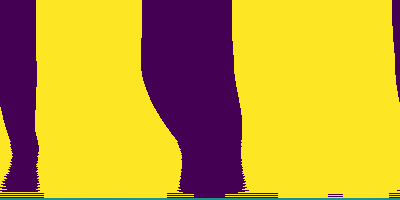
\includegraphics[interpolate=false,width=1.000000in,height=1.000000in]{burgers_rollout_fnn_diff_0.0-img0.png}}%
\end{pgfscope}%
\begin{pgfscope}%
\pgfsetbuttcap%
\pgfsetroundjoin%
\definecolor{currentfill}{rgb}{0.000000,0.000000,0.000000}%
\pgfsetfillcolor{currentfill}%
\pgfsetlinewidth{0.803000pt}%
\definecolor{currentstroke}{rgb}{0.000000,0.000000,0.000000}%
\pgfsetstrokecolor{currentstroke}%
\pgfsetdash{}{0pt}%
\pgfsys@defobject{currentmarker}{\pgfqpoint{0.000000in}{-0.048611in}}{\pgfqpoint{0.000000in}{0.000000in}}{%
\pgfpathmoveto{\pgfqpoint{0.000000in}{0.000000in}}%
\pgfpathlineto{\pgfqpoint{0.000000in}{-0.048611in}}%
\pgfusepath{stroke,fill}%
}%
\begin{pgfscope}%
\pgfsys@transformshift{0.726837in}{0.517039in}%
\pgfsys@useobject{currentmarker}{}%
\end{pgfscope}%
\end{pgfscope}%
\begin{pgfscope}%
\definecolor{textcolor}{rgb}{0.000000,0.000000,0.000000}%
\pgfsetstrokecolor{textcolor}%
\pgfsetfillcolor{textcolor}%
\pgftext[x=0.726837in,y=0.419816in,,top]{\color{textcolor}\rmfamily\fontsize{12.000000}{14.400000}\selectfont 0}%
\end{pgfscope}%
\begin{pgfscope}%
\pgfsetbuttcap%
\pgfsetroundjoin%
\definecolor{currentfill}{rgb}{0.000000,0.000000,0.000000}%
\pgfsetfillcolor{currentfill}%
\pgfsetlinewidth{0.803000pt}%
\definecolor{currentstroke}{rgb}{0.000000,0.000000,0.000000}%
\pgfsetstrokecolor{currentstroke}%
\pgfsetdash{}{0pt}%
\pgfsys@defobject{currentmarker}{\pgfqpoint{0.000000in}{-0.048611in}}{\pgfqpoint{0.000000in}{0.000000in}}{%
\pgfpathmoveto{\pgfqpoint{0.000000in}{0.000000in}}%
\pgfpathlineto{\pgfqpoint{0.000000in}{-0.048611in}}%
\pgfusepath{stroke,fill}%
}%
\begin{pgfscope}%
\pgfsys@transformshift{1.495432in}{0.517039in}%
\pgfsys@useobject{currentmarker}{}%
\end{pgfscope}%
\end{pgfscope}%
\begin{pgfscope}%
\definecolor{textcolor}{rgb}{0.000000,0.000000,0.000000}%
\pgfsetstrokecolor{textcolor}%
\pgfsetfillcolor{textcolor}%
\pgftext[x=1.495432in,y=0.419816in,,top]{\color{textcolor}\rmfamily\fontsize{12.000000}{14.400000}\selectfont 1}%
\end{pgfscope}%
\begin{pgfscope}%
\pgfsetbuttcap%
\pgfsetroundjoin%
\definecolor{currentfill}{rgb}{0.000000,0.000000,0.000000}%
\pgfsetfillcolor{currentfill}%
\pgfsetlinewidth{0.803000pt}%
\definecolor{currentstroke}{rgb}{0.000000,0.000000,0.000000}%
\pgfsetstrokecolor{currentstroke}%
\pgfsetdash{}{0pt}%
\pgfsys@defobject{currentmarker}{\pgfqpoint{0.000000in}{-0.048611in}}{\pgfqpoint{0.000000in}{0.000000in}}{%
\pgfpathmoveto{\pgfqpoint{0.000000in}{0.000000in}}%
\pgfpathlineto{\pgfqpoint{0.000000in}{-0.048611in}}%
\pgfusepath{stroke,fill}%
}%
\begin{pgfscope}%
\pgfsys@transformshift{2.264026in}{0.517039in}%
\pgfsys@useobject{currentmarker}{}%
\end{pgfscope}%
\end{pgfscope}%
\begin{pgfscope}%
\definecolor{textcolor}{rgb}{0.000000,0.000000,0.000000}%
\pgfsetstrokecolor{textcolor}%
\pgfsetfillcolor{textcolor}%
\pgftext[x=2.264026in,y=0.419816in,,top]{\color{textcolor}\rmfamily\fontsize{12.000000}{14.400000}\selectfont 2}%
\end{pgfscope}%
\begin{pgfscope}%
\definecolor{textcolor}{rgb}{0.000000,0.000000,0.000000}%
\pgfsetstrokecolor{textcolor}%
\pgfsetfillcolor{textcolor}%
\pgftext[x=1.495432in,y=0.202965in,,top]{\color{textcolor}\rmfamily\fontsize{12.000000}{14.400000}\selectfont Space}%
\end{pgfscope}%
\begin{pgfscope}%
\pgfsetbuttcap%
\pgfsetroundjoin%
\definecolor{currentfill}{rgb}{0.000000,0.000000,0.000000}%
\pgfsetfillcolor{currentfill}%
\pgfsetlinewidth{0.803000pt}%
\definecolor{currentstroke}{rgb}{0.000000,0.000000,0.000000}%
\pgfsetstrokecolor{currentstroke}%
\pgfsetdash{}{0pt}%
\pgfsys@defobject{currentmarker}{\pgfqpoint{-0.048611in}{0.000000in}}{\pgfqpoint{-0.000000in}{0.000000in}}{%
\pgfpathmoveto{\pgfqpoint{-0.000000in}{0.000000in}}%
\pgfpathlineto{\pgfqpoint{-0.048611in}{0.000000in}}%
\pgfusepath{stroke,fill}%
}%
\begin{pgfscope}%
\pgfsys@transformshift{0.726837in}{0.517039in}%
\pgfsys@useobject{currentmarker}{}%
\end{pgfscope}%
\end{pgfscope}%
\begin{pgfscope}%
\definecolor{textcolor}{rgb}{0.000000,0.000000,0.000000}%
\pgfsetstrokecolor{textcolor}%
\pgfsetfillcolor{textcolor}%
\pgftext[x=0.364559in, y=0.453725in, left, base]{\color{textcolor}\rmfamily\fontsize{12.000000}{14.400000}\selectfont 0.0}%
\end{pgfscope}%
\begin{pgfscope}%
\pgfsetbuttcap%
\pgfsetroundjoin%
\definecolor{currentfill}{rgb}{0.000000,0.000000,0.000000}%
\pgfsetfillcolor{currentfill}%
\pgfsetlinewidth{0.803000pt}%
\definecolor{currentstroke}{rgb}{0.000000,0.000000,0.000000}%
\pgfsetstrokecolor{currentstroke}%
\pgfsetdash{}{0pt}%
\pgfsys@defobject{currentmarker}{\pgfqpoint{-0.048611in}{0.000000in}}{\pgfqpoint{-0.000000in}{0.000000in}}{%
\pgfpathmoveto{\pgfqpoint{-0.000000in}{0.000000in}}%
\pgfpathlineto{\pgfqpoint{-0.048611in}{0.000000in}}%
\pgfusepath{stroke,fill}%
}%
\begin{pgfscope}%
\pgfsys@transformshift{0.726837in}{0.861533in}%
\pgfsys@useobject{currentmarker}{}%
\end{pgfscope}%
\end{pgfscope}%
\begin{pgfscope}%
\definecolor{textcolor}{rgb}{0.000000,0.000000,0.000000}%
\pgfsetstrokecolor{textcolor}%
\pgfsetfillcolor{textcolor}%
\pgftext[x=0.364559in, y=0.798219in, left, base]{\color{textcolor}\rmfamily\fontsize{12.000000}{14.400000}\selectfont 2.5}%
\end{pgfscope}%
\begin{pgfscope}%
\pgfsetbuttcap%
\pgfsetroundjoin%
\definecolor{currentfill}{rgb}{0.000000,0.000000,0.000000}%
\pgfsetfillcolor{currentfill}%
\pgfsetlinewidth{0.803000pt}%
\definecolor{currentstroke}{rgb}{0.000000,0.000000,0.000000}%
\pgfsetstrokecolor{currentstroke}%
\pgfsetdash{}{0pt}%
\pgfsys@defobject{currentmarker}{\pgfqpoint{-0.048611in}{0.000000in}}{\pgfqpoint{-0.000000in}{0.000000in}}{%
\pgfpathmoveto{\pgfqpoint{-0.000000in}{0.000000in}}%
\pgfpathlineto{\pgfqpoint{-0.048611in}{0.000000in}}%
\pgfusepath{stroke,fill}%
}%
\begin{pgfscope}%
\pgfsys@transformshift{0.726837in}{1.206027in}%
\pgfsys@useobject{currentmarker}{}%
\end{pgfscope}%
\end{pgfscope}%
\begin{pgfscope}%
\definecolor{textcolor}{rgb}{0.000000,0.000000,0.000000}%
\pgfsetstrokecolor{textcolor}%
\pgfsetfillcolor{textcolor}%
\pgftext[x=0.364559in, y=1.142714in, left, base]{\color{textcolor}\rmfamily\fontsize{12.000000}{14.400000}\selectfont 5.0}%
\end{pgfscope}%
\begin{pgfscope}%
\pgfsetbuttcap%
\pgfsetroundjoin%
\definecolor{currentfill}{rgb}{0.000000,0.000000,0.000000}%
\pgfsetfillcolor{currentfill}%
\pgfsetlinewidth{0.803000pt}%
\definecolor{currentstroke}{rgb}{0.000000,0.000000,0.000000}%
\pgfsetstrokecolor{currentstroke}%
\pgfsetdash{}{0pt}%
\pgfsys@defobject{currentmarker}{\pgfqpoint{-0.048611in}{0.000000in}}{\pgfqpoint{-0.000000in}{0.000000in}}{%
\pgfpathmoveto{\pgfqpoint{-0.000000in}{0.000000in}}%
\pgfpathlineto{\pgfqpoint{-0.048611in}{0.000000in}}%
\pgfusepath{stroke,fill}%
}%
\begin{pgfscope}%
\pgfsys@transformshift{0.726837in}{1.550522in}%
\pgfsys@useobject{currentmarker}{}%
\end{pgfscope}%
\end{pgfscope}%
\begin{pgfscope}%
\definecolor{textcolor}{rgb}{0.000000,0.000000,0.000000}%
\pgfsetstrokecolor{textcolor}%
\pgfsetfillcolor{textcolor}%
\pgftext[x=0.364559in, y=1.487208in, left, base]{\color{textcolor}\rmfamily\fontsize{12.000000}{14.400000}\selectfont 7.5}%
\end{pgfscope}%
\begin{pgfscope}%
\pgfsetbuttcap%
\pgfsetroundjoin%
\definecolor{currentfill}{rgb}{0.000000,0.000000,0.000000}%
\pgfsetfillcolor{currentfill}%
\pgfsetlinewidth{0.803000pt}%
\definecolor{currentstroke}{rgb}{0.000000,0.000000,0.000000}%
\pgfsetstrokecolor{currentstroke}%
\pgfsetdash{}{0pt}%
\pgfsys@defobject{currentmarker}{\pgfqpoint{-0.048611in}{0.000000in}}{\pgfqpoint{-0.000000in}{0.000000in}}{%
\pgfpathmoveto{\pgfqpoint{-0.000000in}{0.000000in}}%
\pgfpathlineto{\pgfqpoint{-0.048611in}{0.000000in}}%
\pgfusepath{stroke,fill}%
}%
\begin{pgfscope}%
\pgfsys@transformshift{0.726837in}{1.895016in}%
\pgfsys@useobject{currentmarker}{}%
\end{pgfscope}%
\end{pgfscope}%
\begin{pgfscope}%
\definecolor{textcolor}{rgb}{0.000000,0.000000,0.000000}%
\pgfsetstrokecolor{textcolor}%
\pgfsetfillcolor{textcolor}%
\pgftext[x=0.258521in, y=1.831702in, left, base]{\color{textcolor}\rmfamily\fontsize{12.000000}{14.400000}\selectfont 10.0}%
\end{pgfscope}%
\begin{pgfscope}%
\definecolor{textcolor}{rgb}{0.000000,0.000000,0.000000}%
\pgfsetstrokecolor{textcolor}%
\pgfsetfillcolor{textcolor}%
\pgftext[x=0.202965in,y=1.206027in,,bottom,rotate=90.000000]{\color{textcolor}\rmfamily\fontsize{12.000000}{14.400000}\selectfont Time}%
\end{pgfscope}%
\begin{pgfscope}%
\pgfsetrectcap%
\pgfsetmiterjoin%
\pgfsetlinewidth{0.803000pt}%
\definecolor{currentstroke}{rgb}{0.000000,0.000000,0.000000}%
\pgfsetstrokecolor{currentstroke}%
\pgfsetdash{}{0pt}%
\pgfpathmoveto{\pgfqpoint{0.726837in}{0.517039in}}%
\pgfpathlineto{\pgfqpoint{0.726837in}{1.895016in}}%
\pgfusepath{stroke}%
\end{pgfscope}%
\begin{pgfscope}%
\pgfsetrectcap%
\pgfsetmiterjoin%
\pgfsetlinewidth{0.803000pt}%
\definecolor{currentstroke}{rgb}{0.000000,0.000000,0.000000}%
\pgfsetstrokecolor{currentstroke}%
\pgfsetdash{}{0pt}%
\pgfpathmoveto{\pgfqpoint{2.264026in}{0.517039in}}%
\pgfpathlineto{\pgfqpoint{2.264026in}{1.895016in}}%
\pgfusepath{stroke}%
\end{pgfscope}%
\begin{pgfscope}%
\pgfsetrectcap%
\pgfsetmiterjoin%
\pgfsetlinewidth{0.803000pt}%
\definecolor{currentstroke}{rgb}{0.000000,0.000000,0.000000}%
\pgfsetstrokecolor{currentstroke}%
\pgfsetdash{}{0pt}%
\pgfpathmoveto{\pgfqpoint{0.726837in}{0.517039in}}%
\pgfpathlineto{\pgfqpoint{2.264026in}{0.517039in}}%
\pgfusepath{stroke}%
\end{pgfscope}%
\begin{pgfscope}%
\pgfsetrectcap%
\pgfsetmiterjoin%
\pgfsetlinewidth{0.803000pt}%
\definecolor{currentstroke}{rgb}{0.000000,0.000000,0.000000}%
\pgfsetstrokecolor{currentstroke}%
\pgfsetdash{}{0pt}%
\pgfpathmoveto{\pgfqpoint{0.726837in}{1.895016in}}%
\pgfpathlineto{\pgfqpoint{2.264026in}{1.895016in}}%
\pgfusepath{stroke}%
\end{pgfscope}%
\begin{pgfscope}%
\pgfsetbuttcap%
\pgfsetmiterjoin%
\pgfsetlinewidth{0.000000pt}%
\definecolor{currentstroke}{rgb}{0.000000,0.000000,0.000000}%
\pgfsetstrokecolor{currentstroke}%
\pgfsetstrokeopacity{0.000000}%
\pgfsetdash{}{0pt}%
\pgfpathmoveto{\pgfqpoint{2.393905in}{0.517039in}}%
\pgfpathlineto{\pgfqpoint{2.462804in}{0.517039in}}%
\pgfpathlineto{\pgfqpoint{2.462804in}{1.895016in}}%
\pgfpathlineto{\pgfqpoint{2.393905in}{1.895016in}}%
\pgfpathlineto{\pgfqpoint{2.393905in}{0.517039in}}%
\pgfpathclose%
\pgfusepath{}%
\end{pgfscope}%
\begin{pgfscope}%
\pgfsys@transformshift{2.390000in}{0.520000in}%
\pgftext[left,bottom]{
\includegraphics[interpolate=true,width=0.070000in,height=1.380000in]{burgers_rollout_fnn_diff_0.0-img1.png}}%
\end{pgfscope}%
\begin{pgfscope}%
\pgfsetbuttcap%
\pgfsetroundjoin%
\definecolor{currentfill}{rgb}{0.000000,0.000000,0.000000}%
\pgfsetfillcolor{currentfill}%
\pgfsetlinewidth{0.803000pt}%
\definecolor{currentstroke}{rgb}{0.000000,0.000000,0.000000}%
\pgfsetstrokecolor{currentstroke}%
\pgfsetdash{}{0pt}%
\pgfsys@defobject{currentmarker}{\pgfqpoint{0.000000in}{0.000000in}}{\pgfqpoint{0.048611in}{0.000000in}}{%
\pgfpathmoveto{\pgfqpoint{0.000000in}{0.000000in}}%
\pgfpathlineto{\pgfqpoint{0.048611in}{0.000000in}}%
\pgfusepath{stroke,fill}%
}%
\begin{pgfscope}%
\pgfsys@transformshift{2.462804in}{0.839076in}%
\pgfsys@useobject{currentmarker}{}%
\end{pgfscope}%
\end{pgfscope}%
\begin{pgfscope}%
\definecolor{textcolor}{rgb}{0.000000,0.000000,0.000000}%
\pgfsetstrokecolor{textcolor}%
\pgfsetfillcolor{textcolor}%
\pgftext[x=2.560026in, y=0.775762in, left, base]{\color{textcolor}\rmfamily\fontsize{12.000000}{14.400000}\selectfont \ensuremath{-}0.5}%
\end{pgfscope}%
\begin{pgfscope}%
\pgfsetbuttcap%
\pgfsetroundjoin%
\definecolor{currentfill}{rgb}{0.000000,0.000000,0.000000}%
\pgfsetfillcolor{currentfill}%
\pgfsetlinewidth{0.803000pt}%
\definecolor{currentstroke}{rgb}{0.000000,0.000000,0.000000}%
\pgfsetstrokecolor{currentstroke}%
\pgfsetdash{}{0pt}%
\pgfsys@defobject{currentmarker}{\pgfqpoint{0.000000in}{0.000000in}}{\pgfqpoint{0.048611in}{0.000000in}}{%
\pgfpathmoveto{\pgfqpoint{0.000000in}{0.000000in}}%
\pgfpathlineto{\pgfqpoint{0.048611in}{0.000000in}}%
\pgfusepath{stroke,fill}%
}%
\begin{pgfscope}%
\pgfsys@transformshift{2.462804in}{1.206027in}%
\pgfsys@useobject{currentmarker}{}%
\end{pgfscope}%
\end{pgfscope}%
\begin{pgfscope}%
\definecolor{textcolor}{rgb}{0.000000,0.000000,0.000000}%
\pgfsetstrokecolor{textcolor}%
\pgfsetfillcolor{textcolor}%
\pgftext[x=2.560026in, y=1.142714in, left, base]{\color{textcolor}\rmfamily\fontsize{12.000000}{14.400000}\selectfont 0.0}%
\end{pgfscope}%
\begin{pgfscope}%
\pgfsetbuttcap%
\pgfsetroundjoin%
\definecolor{currentfill}{rgb}{0.000000,0.000000,0.000000}%
\pgfsetfillcolor{currentfill}%
\pgfsetlinewidth{0.803000pt}%
\definecolor{currentstroke}{rgb}{0.000000,0.000000,0.000000}%
\pgfsetstrokecolor{currentstroke}%
\pgfsetdash{}{0pt}%
\pgfsys@defobject{currentmarker}{\pgfqpoint{0.000000in}{0.000000in}}{\pgfqpoint{0.048611in}{0.000000in}}{%
\pgfpathmoveto{\pgfqpoint{0.000000in}{0.000000in}}%
\pgfpathlineto{\pgfqpoint{0.048611in}{0.000000in}}%
\pgfusepath{stroke,fill}%
}%
\begin{pgfscope}%
\pgfsys@transformshift{2.462804in}{1.572979in}%
\pgfsys@useobject{currentmarker}{}%
\end{pgfscope}%
\end{pgfscope}%
\begin{pgfscope}%
\definecolor{textcolor}{rgb}{0.000000,0.000000,0.000000}%
\pgfsetstrokecolor{textcolor}%
\pgfsetfillcolor{textcolor}%
\pgftext[x=2.560026in, y=1.509665in, left, base]{\color{textcolor}\rmfamily\fontsize{12.000000}{14.400000}\selectfont 0.5}%
\end{pgfscope}%
\begin{pgfscope}%
\pgfsetrectcap%
\pgfsetmiterjoin%
\pgfsetlinewidth{0.803000pt}%
\definecolor{currentstroke}{rgb}{0.000000,0.000000,0.000000}%
\pgfsetstrokecolor{currentstroke}%
\pgfsetdash{}{0pt}%
\pgfpathmoveto{\pgfqpoint{2.393905in}{0.517039in}}%
\pgfpathlineto{\pgfqpoint{2.428354in}{0.517039in}}%
\pgfpathlineto{\pgfqpoint{2.462804in}{0.517039in}}%
\pgfpathlineto{\pgfqpoint{2.462804in}{1.895016in}}%
\pgfpathlineto{\pgfqpoint{2.428354in}{1.895016in}}%
\pgfpathlineto{\pgfqpoint{2.393905in}{1.895016in}}%
\pgfpathlineto{\pgfqpoint{2.393905in}{0.517039in}}%
\pgfpathclose%
\pgfusepath{stroke}%
\end{pgfscope}%
\end{pgfpicture}%
\makeatother%
\endgroup%

      \end{adjustbox}
      \caption{SpectralSVR difference with target.}\label{fig:comp_fnn_diff_0.0}
    \end{subfigure}
    \begin{subfigure}{0.49\linewidth}
      \begin{adjustbox}{width=\linewidth}
        \begingroup%
\makeatletter%
\begin{pgfpicture}%
\pgfpathrectangle{\pgfpointorigin}{\pgfqpoint{3.000000in}{2.000000in}}%
\pgfusepath{use as bounding box, clip}%
\begin{pgfscope}%
\pgfsetbuttcap%
\pgfsetmiterjoin%
\pgfsetlinewidth{0.000000pt}%
\definecolor{currentstroke}{rgb}{0.000000,0.000000,0.000000}%
\pgfsetstrokecolor{currentstroke}%
\pgfsetstrokeopacity{0.000000}%
\pgfsetdash{}{0pt}%
\pgfpathmoveto{\pgfqpoint{0.000000in}{0.000000in}}%
\pgfpathlineto{\pgfqpoint{3.000000in}{0.000000in}}%
\pgfpathlineto{\pgfqpoint{3.000000in}{2.000000in}}%
\pgfpathlineto{\pgfqpoint{0.000000in}{2.000000in}}%
\pgfpathlineto{\pgfqpoint{0.000000in}{0.000000in}}%
\pgfpathclose%
\pgfusepath{}%
\end{pgfscope}%
\begin{pgfscope}%
\pgfsetbuttcap%
\pgfsetmiterjoin%
\pgfsetlinewidth{0.000000pt}%
\definecolor{currentstroke}{rgb}{0.000000,0.000000,0.000000}%
\pgfsetstrokecolor{currentstroke}%
\pgfsetstrokeopacity{0.000000}%
\pgfsetdash{}{0pt}%
\pgfpathmoveto{\pgfqpoint{0.726837in}{0.517039in}}%
\pgfpathlineto{\pgfqpoint{2.263621in}{0.517039in}}%
\pgfpathlineto{\pgfqpoint{2.263621in}{1.895016in}}%
\pgfpathlineto{\pgfqpoint{0.726837in}{1.895016in}}%
\pgfpathlineto{\pgfqpoint{0.726837in}{0.517039in}}%
\pgfpathclose%
\pgfusepath{}%
\end{pgfscope}%
\begin{pgfscope}%
\pgfpathrectangle{\pgfqpoint{0.726837in}{0.517039in}}{\pgfqpoint{1.536784in}{1.377978in}}%
\pgfusepath{clip}%
\pgfsys@transformcm{1.536784}{0.000000}{0.000000}{1.377978}{0.726837in}{0.517039in}%
\pgftext[left,bottom]{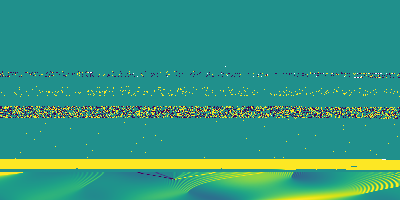
\includegraphics[interpolate=false,width=1.000000in,height=1.000000in]{burgers_rollout_spo_pred_0.0-img0.png}}%
\end{pgfscope}%
\begin{pgfscope}%
\pgfsetbuttcap%
\pgfsetroundjoin%
\definecolor{currentfill}{rgb}{0.000000,0.000000,0.000000}%
\pgfsetfillcolor{currentfill}%
\pgfsetlinewidth{0.803000pt}%
\definecolor{currentstroke}{rgb}{0.000000,0.000000,0.000000}%
\pgfsetstrokecolor{currentstroke}%
\pgfsetdash{}{0pt}%
\pgfsys@defobject{currentmarker}{\pgfqpoint{0.000000in}{-0.048611in}}{\pgfqpoint{0.000000in}{0.000000in}}{%
\pgfpathmoveto{\pgfqpoint{0.000000in}{0.000000in}}%
\pgfpathlineto{\pgfqpoint{0.000000in}{-0.048611in}}%
\pgfusepath{stroke,fill}%
}%
\begin{pgfscope}%
\pgfsys@transformshift{0.726837in}{0.517039in}%
\pgfsys@useobject{currentmarker}{}%
\end{pgfscope}%
\end{pgfscope}%
\begin{pgfscope}%
\definecolor{textcolor}{rgb}{0.000000,0.000000,0.000000}%
\pgfsetstrokecolor{textcolor}%
\pgfsetfillcolor{textcolor}%
\pgftext[x=0.726837in,y=0.419816in,,top]{\color{textcolor}\rmfamily\fontsize{12.000000}{14.400000}\selectfont 0}%
\end{pgfscope}%
\begin{pgfscope}%
\pgfsetbuttcap%
\pgfsetroundjoin%
\definecolor{currentfill}{rgb}{0.000000,0.000000,0.000000}%
\pgfsetfillcolor{currentfill}%
\pgfsetlinewidth{0.803000pt}%
\definecolor{currentstroke}{rgb}{0.000000,0.000000,0.000000}%
\pgfsetstrokecolor{currentstroke}%
\pgfsetdash{}{0pt}%
\pgfsys@defobject{currentmarker}{\pgfqpoint{0.000000in}{-0.048611in}}{\pgfqpoint{0.000000in}{0.000000in}}{%
\pgfpathmoveto{\pgfqpoint{0.000000in}{0.000000in}}%
\pgfpathlineto{\pgfqpoint{0.000000in}{-0.048611in}}%
\pgfusepath{stroke,fill}%
}%
\begin{pgfscope}%
\pgfsys@transformshift{1.495229in}{0.517039in}%
\pgfsys@useobject{currentmarker}{}%
\end{pgfscope}%
\end{pgfscope}%
\begin{pgfscope}%
\definecolor{textcolor}{rgb}{0.000000,0.000000,0.000000}%
\pgfsetstrokecolor{textcolor}%
\pgfsetfillcolor{textcolor}%
\pgftext[x=1.495229in,y=0.419816in,,top]{\color{textcolor}\rmfamily\fontsize{12.000000}{14.400000}\selectfont 1}%
\end{pgfscope}%
\begin{pgfscope}%
\pgfsetbuttcap%
\pgfsetroundjoin%
\definecolor{currentfill}{rgb}{0.000000,0.000000,0.000000}%
\pgfsetfillcolor{currentfill}%
\pgfsetlinewidth{0.803000pt}%
\definecolor{currentstroke}{rgb}{0.000000,0.000000,0.000000}%
\pgfsetstrokecolor{currentstroke}%
\pgfsetdash{}{0pt}%
\pgfsys@defobject{currentmarker}{\pgfqpoint{0.000000in}{-0.048611in}}{\pgfqpoint{0.000000in}{0.000000in}}{%
\pgfpathmoveto{\pgfqpoint{0.000000in}{0.000000in}}%
\pgfpathlineto{\pgfqpoint{0.000000in}{-0.048611in}}%
\pgfusepath{stroke,fill}%
}%
\begin{pgfscope}%
\pgfsys@transformshift{2.263621in}{0.517039in}%
\pgfsys@useobject{currentmarker}{}%
\end{pgfscope}%
\end{pgfscope}%
\begin{pgfscope}%
\definecolor{textcolor}{rgb}{0.000000,0.000000,0.000000}%
\pgfsetstrokecolor{textcolor}%
\pgfsetfillcolor{textcolor}%
\pgftext[x=2.263621in,y=0.419816in,,top]{\color{textcolor}\rmfamily\fontsize{12.000000}{14.400000}\selectfont 2}%
\end{pgfscope}%
\begin{pgfscope}%
\definecolor{textcolor}{rgb}{0.000000,0.000000,0.000000}%
\pgfsetstrokecolor{textcolor}%
\pgfsetfillcolor{textcolor}%
\pgftext[x=1.495229in,y=0.202965in,,top]{\color{textcolor}\rmfamily\fontsize{12.000000}{14.400000}\selectfont Space}%
\end{pgfscope}%
\begin{pgfscope}%
\pgfsetbuttcap%
\pgfsetroundjoin%
\definecolor{currentfill}{rgb}{0.000000,0.000000,0.000000}%
\pgfsetfillcolor{currentfill}%
\pgfsetlinewidth{0.803000pt}%
\definecolor{currentstroke}{rgb}{0.000000,0.000000,0.000000}%
\pgfsetstrokecolor{currentstroke}%
\pgfsetdash{}{0pt}%
\pgfsys@defobject{currentmarker}{\pgfqpoint{-0.048611in}{0.000000in}}{\pgfqpoint{-0.000000in}{0.000000in}}{%
\pgfpathmoveto{\pgfqpoint{-0.000000in}{0.000000in}}%
\pgfpathlineto{\pgfqpoint{-0.048611in}{0.000000in}}%
\pgfusepath{stroke,fill}%
}%
\begin{pgfscope}%
\pgfsys@transformshift{0.726837in}{0.517039in}%
\pgfsys@useobject{currentmarker}{}%
\end{pgfscope}%
\end{pgfscope}%
\begin{pgfscope}%
\definecolor{textcolor}{rgb}{0.000000,0.000000,0.000000}%
\pgfsetstrokecolor{textcolor}%
\pgfsetfillcolor{textcolor}%
\pgftext[x=0.364559in, y=0.453725in, left, base]{\color{textcolor}\rmfamily\fontsize{12.000000}{14.400000}\selectfont 0.0}%
\end{pgfscope}%
\begin{pgfscope}%
\pgfsetbuttcap%
\pgfsetroundjoin%
\definecolor{currentfill}{rgb}{0.000000,0.000000,0.000000}%
\pgfsetfillcolor{currentfill}%
\pgfsetlinewidth{0.803000pt}%
\definecolor{currentstroke}{rgb}{0.000000,0.000000,0.000000}%
\pgfsetstrokecolor{currentstroke}%
\pgfsetdash{}{0pt}%
\pgfsys@defobject{currentmarker}{\pgfqpoint{-0.048611in}{0.000000in}}{\pgfqpoint{-0.000000in}{0.000000in}}{%
\pgfpathmoveto{\pgfqpoint{-0.000000in}{0.000000in}}%
\pgfpathlineto{\pgfqpoint{-0.048611in}{0.000000in}}%
\pgfusepath{stroke,fill}%
}%
\begin{pgfscope}%
\pgfsys@transformshift{0.726837in}{0.861533in}%
\pgfsys@useobject{currentmarker}{}%
\end{pgfscope}%
\end{pgfscope}%
\begin{pgfscope}%
\definecolor{textcolor}{rgb}{0.000000,0.000000,0.000000}%
\pgfsetstrokecolor{textcolor}%
\pgfsetfillcolor{textcolor}%
\pgftext[x=0.364559in, y=0.798219in, left, base]{\color{textcolor}\rmfamily\fontsize{12.000000}{14.400000}\selectfont 2.5}%
\end{pgfscope}%
\begin{pgfscope}%
\pgfsetbuttcap%
\pgfsetroundjoin%
\definecolor{currentfill}{rgb}{0.000000,0.000000,0.000000}%
\pgfsetfillcolor{currentfill}%
\pgfsetlinewidth{0.803000pt}%
\definecolor{currentstroke}{rgb}{0.000000,0.000000,0.000000}%
\pgfsetstrokecolor{currentstroke}%
\pgfsetdash{}{0pt}%
\pgfsys@defobject{currentmarker}{\pgfqpoint{-0.048611in}{0.000000in}}{\pgfqpoint{-0.000000in}{0.000000in}}{%
\pgfpathmoveto{\pgfqpoint{-0.000000in}{0.000000in}}%
\pgfpathlineto{\pgfqpoint{-0.048611in}{0.000000in}}%
\pgfusepath{stroke,fill}%
}%
\begin{pgfscope}%
\pgfsys@transformshift{0.726837in}{1.206027in}%
\pgfsys@useobject{currentmarker}{}%
\end{pgfscope}%
\end{pgfscope}%
\begin{pgfscope}%
\definecolor{textcolor}{rgb}{0.000000,0.000000,0.000000}%
\pgfsetstrokecolor{textcolor}%
\pgfsetfillcolor{textcolor}%
\pgftext[x=0.364559in, y=1.142714in, left, base]{\color{textcolor}\rmfamily\fontsize{12.000000}{14.400000}\selectfont 5.0}%
\end{pgfscope}%
\begin{pgfscope}%
\pgfsetbuttcap%
\pgfsetroundjoin%
\definecolor{currentfill}{rgb}{0.000000,0.000000,0.000000}%
\pgfsetfillcolor{currentfill}%
\pgfsetlinewidth{0.803000pt}%
\definecolor{currentstroke}{rgb}{0.000000,0.000000,0.000000}%
\pgfsetstrokecolor{currentstroke}%
\pgfsetdash{}{0pt}%
\pgfsys@defobject{currentmarker}{\pgfqpoint{-0.048611in}{0.000000in}}{\pgfqpoint{-0.000000in}{0.000000in}}{%
\pgfpathmoveto{\pgfqpoint{-0.000000in}{0.000000in}}%
\pgfpathlineto{\pgfqpoint{-0.048611in}{0.000000in}}%
\pgfusepath{stroke,fill}%
}%
\begin{pgfscope}%
\pgfsys@transformshift{0.726837in}{1.550522in}%
\pgfsys@useobject{currentmarker}{}%
\end{pgfscope}%
\end{pgfscope}%
\begin{pgfscope}%
\definecolor{textcolor}{rgb}{0.000000,0.000000,0.000000}%
\pgfsetstrokecolor{textcolor}%
\pgfsetfillcolor{textcolor}%
\pgftext[x=0.364559in, y=1.487208in, left, base]{\color{textcolor}\rmfamily\fontsize{12.000000}{14.400000}\selectfont 7.5}%
\end{pgfscope}%
\begin{pgfscope}%
\pgfsetbuttcap%
\pgfsetroundjoin%
\definecolor{currentfill}{rgb}{0.000000,0.000000,0.000000}%
\pgfsetfillcolor{currentfill}%
\pgfsetlinewidth{0.803000pt}%
\definecolor{currentstroke}{rgb}{0.000000,0.000000,0.000000}%
\pgfsetstrokecolor{currentstroke}%
\pgfsetdash{}{0pt}%
\pgfsys@defobject{currentmarker}{\pgfqpoint{-0.048611in}{0.000000in}}{\pgfqpoint{-0.000000in}{0.000000in}}{%
\pgfpathmoveto{\pgfqpoint{-0.000000in}{0.000000in}}%
\pgfpathlineto{\pgfqpoint{-0.048611in}{0.000000in}}%
\pgfusepath{stroke,fill}%
}%
\begin{pgfscope}%
\pgfsys@transformshift{0.726837in}{1.895016in}%
\pgfsys@useobject{currentmarker}{}%
\end{pgfscope}%
\end{pgfscope}%
\begin{pgfscope}%
\definecolor{textcolor}{rgb}{0.000000,0.000000,0.000000}%
\pgfsetstrokecolor{textcolor}%
\pgfsetfillcolor{textcolor}%
\pgftext[x=0.258521in, y=1.831702in, left, base]{\color{textcolor}\rmfamily\fontsize{12.000000}{14.400000}\selectfont 10.0}%
\end{pgfscope}%
\begin{pgfscope}%
\definecolor{textcolor}{rgb}{0.000000,0.000000,0.000000}%
\pgfsetstrokecolor{textcolor}%
\pgfsetfillcolor{textcolor}%
\pgftext[x=0.202965in,y=1.206027in,,bottom,rotate=90.000000]{\color{textcolor}\rmfamily\fontsize{12.000000}{14.400000}\selectfont Time}%
\end{pgfscope}%
\begin{pgfscope}%
\pgfsetrectcap%
\pgfsetmiterjoin%
\pgfsetlinewidth{0.803000pt}%
\definecolor{currentstroke}{rgb}{0.000000,0.000000,0.000000}%
\pgfsetstrokecolor{currentstroke}%
\pgfsetdash{}{0pt}%
\pgfpathmoveto{\pgfqpoint{0.726837in}{0.517039in}}%
\pgfpathlineto{\pgfqpoint{0.726837in}{1.895016in}}%
\pgfusepath{stroke}%
\end{pgfscope}%
\begin{pgfscope}%
\pgfsetrectcap%
\pgfsetmiterjoin%
\pgfsetlinewidth{0.803000pt}%
\definecolor{currentstroke}{rgb}{0.000000,0.000000,0.000000}%
\pgfsetstrokecolor{currentstroke}%
\pgfsetdash{}{0pt}%
\pgfpathmoveto{\pgfqpoint{2.263621in}{0.517039in}}%
\pgfpathlineto{\pgfqpoint{2.263621in}{1.895016in}}%
\pgfusepath{stroke}%
\end{pgfscope}%
\begin{pgfscope}%
\pgfsetrectcap%
\pgfsetmiterjoin%
\pgfsetlinewidth{0.803000pt}%
\definecolor{currentstroke}{rgb}{0.000000,0.000000,0.000000}%
\pgfsetstrokecolor{currentstroke}%
\pgfsetdash{}{0pt}%
\pgfpathmoveto{\pgfqpoint{0.726837in}{0.517039in}}%
\pgfpathlineto{\pgfqpoint{2.263621in}{0.517039in}}%
\pgfusepath{stroke}%
\end{pgfscope}%
\begin{pgfscope}%
\pgfsetrectcap%
\pgfsetmiterjoin%
\pgfsetlinewidth{0.803000pt}%
\definecolor{currentstroke}{rgb}{0.000000,0.000000,0.000000}%
\pgfsetstrokecolor{currentstroke}%
\pgfsetdash{}{0pt}%
\pgfpathmoveto{\pgfqpoint{0.726837in}{1.895016in}}%
\pgfpathlineto{\pgfqpoint{2.263621in}{1.895016in}}%
\pgfusepath{stroke}%
\end{pgfscope}%
\begin{pgfscope}%
\pgfsetbuttcap%
\pgfsetmiterjoin%
\pgfsetlinewidth{0.000000pt}%
\definecolor{currentstroke}{rgb}{0.000000,0.000000,0.000000}%
\pgfsetstrokecolor{currentstroke}%
\pgfsetstrokeopacity{0.000000}%
\pgfsetdash{}{0pt}%
\pgfpathmoveto{\pgfqpoint{2.393479in}{0.517039in}}%
\pgfpathlineto{\pgfqpoint{2.462378in}{0.517039in}}%
\pgfpathlineto{\pgfqpoint{2.462378in}{1.895016in}}%
\pgfpathlineto{\pgfqpoint{2.393479in}{1.895016in}}%
\pgfpathlineto{\pgfqpoint{2.393479in}{0.517039in}}%
\pgfpathclose%
\pgfusepath{}%
\end{pgfscope}%
\begin{pgfscope}%
\pgfsys@transformshift{2.390000in}{0.520000in}%
\pgftext[left,bottom]{
\includegraphics[interpolate=true,width=0.070000in,height=1.380000in]{burgers_rollout_spo_pred_0.0-img1.png}}%
\end{pgfscope}%
\begin{pgfscope}%
\pgfsetbuttcap%
\pgfsetroundjoin%
\definecolor{currentfill}{rgb}{0.000000,0.000000,0.000000}%
\pgfsetfillcolor{currentfill}%
\pgfsetlinewidth{0.803000pt}%
\definecolor{currentstroke}{rgb}{0.000000,0.000000,0.000000}%
\pgfsetstrokecolor{currentstroke}%
\pgfsetdash{}{0pt}%
\pgfsys@defobject{currentmarker}{\pgfqpoint{0.000000in}{0.000000in}}{\pgfqpoint{0.048611in}{0.000000in}}{%
\pgfpathmoveto{\pgfqpoint{0.000000in}{0.000000in}}%
\pgfpathlineto{\pgfqpoint{0.048611in}{0.000000in}}%
\pgfusepath{stroke,fill}%
}%
\begin{pgfscope}%
\pgfsys@transformshift{2.462378in}{0.839076in}%
\pgfsys@useobject{currentmarker}{}%
\end{pgfscope}%
\end{pgfscope}%
\begin{pgfscope}%
\definecolor{textcolor}{rgb}{0.000000,0.000000,0.000000}%
\pgfsetstrokecolor{textcolor}%
\pgfsetfillcolor{textcolor}%
\pgftext[x=2.559601in, y=0.775762in, left, base]{\color{textcolor}\rmfamily\fontsize{12.000000}{14.400000}\selectfont \ensuremath{-}0.5}%
\end{pgfscope}%
\begin{pgfscope}%
\pgfsetbuttcap%
\pgfsetroundjoin%
\definecolor{currentfill}{rgb}{0.000000,0.000000,0.000000}%
\pgfsetfillcolor{currentfill}%
\pgfsetlinewidth{0.803000pt}%
\definecolor{currentstroke}{rgb}{0.000000,0.000000,0.000000}%
\pgfsetstrokecolor{currentstroke}%
\pgfsetdash{}{0pt}%
\pgfsys@defobject{currentmarker}{\pgfqpoint{0.000000in}{0.000000in}}{\pgfqpoint{0.048611in}{0.000000in}}{%
\pgfpathmoveto{\pgfqpoint{0.000000in}{0.000000in}}%
\pgfpathlineto{\pgfqpoint{0.048611in}{0.000000in}}%
\pgfusepath{stroke,fill}%
}%
\begin{pgfscope}%
\pgfsys@transformshift{2.462378in}{1.206027in}%
\pgfsys@useobject{currentmarker}{}%
\end{pgfscope}%
\end{pgfscope}%
\begin{pgfscope}%
\definecolor{textcolor}{rgb}{0.000000,0.000000,0.000000}%
\pgfsetstrokecolor{textcolor}%
\pgfsetfillcolor{textcolor}%
\pgftext[x=2.559601in, y=1.142714in, left, base]{\color{textcolor}\rmfamily\fontsize{12.000000}{14.400000}\selectfont 0.0}%
\end{pgfscope}%
\begin{pgfscope}%
\pgfsetbuttcap%
\pgfsetroundjoin%
\definecolor{currentfill}{rgb}{0.000000,0.000000,0.000000}%
\pgfsetfillcolor{currentfill}%
\pgfsetlinewidth{0.803000pt}%
\definecolor{currentstroke}{rgb}{0.000000,0.000000,0.000000}%
\pgfsetstrokecolor{currentstroke}%
\pgfsetdash{}{0pt}%
\pgfsys@defobject{currentmarker}{\pgfqpoint{0.000000in}{0.000000in}}{\pgfqpoint{0.048611in}{0.000000in}}{%
\pgfpathmoveto{\pgfqpoint{0.000000in}{0.000000in}}%
\pgfpathlineto{\pgfqpoint{0.048611in}{0.000000in}}%
\pgfusepath{stroke,fill}%
}%
\begin{pgfscope}%
\pgfsys@transformshift{2.462378in}{1.572979in}%
\pgfsys@useobject{currentmarker}{}%
\end{pgfscope}%
\end{pgfscope}%
\begin{pgfscope}%
\definecolor{textcolor}{rgb}{0.000000,0.000000,0.000000}%
\pgfsetstrokecolor{textcolor}%
\pgfsetfillcolor{textcolor}%
\pgftext[x=2.559601in, y=1.509665in, left, base]{\color{textcolor}\rmfamily\fontsize{12.000000}{14.400000}\selectfont 0.5}%
\end{pgfscope}%
\begin{pgfscope}%
\pgfsetrectcap%
\pgfsetmiterjoin%
\pgfsetlinewidth{0.803000pt}%
\definecolor{currentstroke}{rgb}{0.000000,0.000000,0.000000}%
\pgfsetstrokecolor{currentstroke}%
\pgfsetdash{}{0pt}%
\pgfpathmoveto{\pgfqpoint{2.393479in}{0.517039in}}%
\pgfpathlineto{\pgfqpoint{2.427929in}{0.517039in}}%
\pgfpathlineto{\pgfqpoint{2.462378in}{0.517039in}}%
\pgfpathlineto{\pgfqpoint{2.462378in}{1.895016in}}%
\pgfpathlineto{\pgfqpoint{2.427929in}{1.895016in}}%
\pgfpathlineto{\pgfqpoint{2.393479in}{1.895016in}}%
\pgfpathlineto{\pgfqpoint{2.393479in}{0.517039in}}%
\pgfpathclose%
\pgfusepath{stroke}%
\end{pgfscope}%
\end{pgfpicture}%
\makeatother%
\endgroup%

      \end{adjustbox}
      \caption{lsoda prediction.}\label{fig:comp_spo_pred_0.0}
    \end{subfigure}
    \begin{subfigure}{0.49\linewidth}
      \begin{adjustbox}{width=\linewidth}
        \begingroup%
\makeatletter%
\begin{pgfpicture}%
\pgfpathrectangle{\pgfpointorigin}{\pgfqpoint{3.000000in}{2.000000in}}%
\pgfusepath{use as bounding box, clip}%
\begin{pgfscope}%
\pgfsetbuttcap%
\pgfsetmiterjoin%
\pgfsetlinewidth{0.000000pt}%
\definecolor{currentstroke}{rgb}{0.000000,0.000000,0.000000}%
\pgfsetstrokecolor{currentstroke}%
\pgfsetstrokeopacity{0.000000}%
\pgfsetdash{}{0pt}%
\pgfpathmoveto{\pgfqpoint{0.000000in}{0.000000in}}%
\pgfpathlineto{\pgfqpoint{3.000000in}{0.000000in}}%
\pgfpathlineto{\pgfqpoint{3.000000in}{2.000000in}}%
\pgfpathlineto{\pgfqpoint{0.000000in}{2.000000in}}%
\pgfpathlineto{\pgfqpoint{0.000000in}{0.000000in}}%
\pgfpathclose%
\pgfusepath{}%
\end{pgfscope}%
\begin{pgfscope}%
\pgfsetbuttcap%
\pgfsetmiterjoin%
\pgfsetlinewidth{0.000000pt}%
\definecolor{currentstroke}{rgb}{0.000000,0.000000,0.000000}%
\pgfsetstrokecolor{currentstroke}%
\pgfsetstrokeopacity{0.000000}%
\pgfsetdash{}{0pt}%
\pgfpathmoveto{\pgfqpoint{0.726837in}{0.517039in}}%
\pgfpathlineto{\pgfqpoint{2.263621in}{0.517039in}}%
\pgfpathlineto{\pgfqpoint{2.263621in}{1.895016in}}%
\pgfpathlineto{\pgfqpoint{0.726837in}{1.895016in}}%
\pgfpathlineto{\pgfqpoint{0.726837in}{0.517039in}}%
\pgfpathclose%
\pgfusepath{}%
\end{pgfscope}%
\begin{pgfscope}%
\pgfpathrectangle{\pgfqpoint{0.726837in}{0.517039in}}{\pgfqpoint{1.536784in}{1.377978in}}%
\pgfusepath{clip}%
\pgfsys@transformcm{1.536784}{0.000000}{0.000000}{1.377978}{0.726837in}{0.517039in}%
\pgftext[left,bottom]{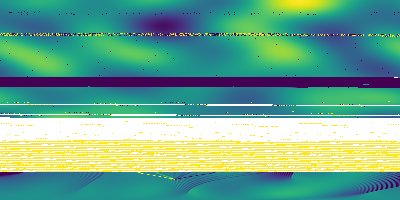
\includegraphics[interpolate=false,width=1.000000in,height=1.000000in]{burgers_rollout_spo_diff_0.0-img0.png}}%
\end{pgfscope}%
\begin{pgfscope}%
\pgfsetbuttcap%
\pgfsetroundjoin%
\definecolor{currentfill}{rgb}{0.000000,0.000000,0.000000}%
\pgfsetfillcolor{currentfill}%
\pgfsetlinewidth{0.803000pt}%
\definecolor{currentstroke}{rgb}{0.000000,0.000000,0.000000}%
\pgfsetstrokecolor{currentstroke}%
\pgfsetdash{}{0pt}%
\pgfsys@defobject{currentmarker}{\pgfqpoint{0.000000in}{-0.048611in}}{\pgfqpoint{0.000000in}{0.000000in}}{%
\pgfpathmoveto{\pgfqpoint{0.000000in}{0.000000in}}%
\pgfpathlineto{\pgfqpoint{0.000000in}{-0.048611in}}%
\pgfusepath{stroke,fill}%
}%
\begin{pgfscope}%
\pgfsys@transformshift{0.726837in}{0.517039in}%
\pgfsys@useobject{currentmarker}{}%
\end{pgfscope}%
\end{pgfscope}%
\begin{pgfscope}%
\definecolor{textcolor}{rgb}{0.000000,0.000000,0.000000}%
\pgfsetstrokecolor{textcolor}%
\pgfsetfillcolor{textcolor}%
\pgftext[x=0.726837in,y=0.419816in,,top]{\color{textcolor}\rmfamily\fontsize{12.000000}{14.400000}\selectfont 0}%
\end{pgfscope}%
\begin{pgfscope}%
\pgfsetbuttcap%
\pgfsetroundjoin%
\definecolor{currentfill}{rgb}{0.000000,0.000000,0.000000}%
\pgfsetfillcolor{currentfill}%
\pgfsetlinewidth{0.803000pt}%
\definecolor{currentstroke}{rgb}{0.000000,0.000000,0.000000}%
\pgfsetstrokecolor{currentstroke}%
\pgfsetdash{}{0pt}%
\pgfsys@defobject{currentmarker}{\pgfqpoint{0.000000in}{-0.048611in}}{\pgfqpoint{0.000000in}{0.000000in}}{%
\pgfpathmoveto{\pgfqpoint{0.000000in}{0.000000in}}%
\pgfpathlineto{\pgfqpoint{0.000000in}{-0.048611in}}%
\pgfusepath{stroke,fill}%
}%
\begin{pgfscope}%
\pgfsys@transformshift{1.495229in}{0.517039in}%
\pgfsys@useobject{currentmarker}{}%
\end{pgfscope}%
\end{pgfscope}%
\begin{pgfscope}%
\definecolor{textcolor}{rgb}{0.000000,0.000000,0.000000}%
\pgfsetstrokecolor{textcolor}%
\pgfsetfillcolor{textcolor}%
\pgftext[x=1.495229in,y=0.419816in,,top]{\color{textcolor}\rmfamily\fontsize{12.000000}{14.400000}\selectfont 1}%
\end{pgfscope}%
\begin{pgfscope}%
\pgfsetbuttcap%
\pgfsetroundjoin%
\definecolor{currentfill}{rgb}{0.000000,0.000000,0.000000}%
\pgfsetfillcolor{currentfill}%
\pgfsetlinewidth{0.803000pt}%
\definecolor{currentstroke}{rgb}{0.000000,0.000000,0.000000}%
\pgfsetstrokecolor{currentstroke}%
\pgfsetdash{}{0pt}%
\pgfsys@defobject{currentmarker}{\pgfqpoint{0.000000in}{-0.048611in}}{\pgfqpoint{0.000000in}{0.000000in}}{%
\pgfpathmoveto{\pgfqpoint{0.000000in}{0.000000in}}%
\pgfpathlineto{\pgfqpoint{0.000000in}{-0.048611in}}%
\pgfusepath{stroke,fill}%
}%
\begin{pgfscope}%
\pgfsys@transformshift{2.263621in}{0.517039in}%
\pgfsys@useobject{currentmarker}{}%
\end{pgfscope}%
\end{pgfscope}%
\begin{pgfscope}%
\definecolor{textcolor}{rgb}{0.000000,0.000000,0.000000}%
\pgfsetstrokecolor{textcolor}%
\pgfsetfillcolor{textcolor}%
\pgftext[x=2.263621in,y=0.419816in,,top]{\color{textcolor}\rmfamily\fontsize{12.000000}{14.400000}\selectfont 2}%
\end{pgfscope}%
\begin{pgfscope}%
\definecolor{textcolor}{rgb}{0.000000,0.000000,0.000000}%
\pgfsetstrokecolor{textcolor}%
\pgfsetfillcolor{textcolor}%
\pgftext[x=1.495229in,y=0.202965in,,top]{\color{textcolor}\rmfamily\fontsize{12.000000}{14.400000}\selectfont Space}%
\end{pgfscope}%
\begin{pgfscope}%
\pgfsetbuttcap%
\pgfsetroundjoin%
\definecolor{currentfill}{rgb}{0.000000,0.000000,0.000000}%
\pgfsetfillcolor{currentfill}%
\pgfsetlinewidth{0.803000pt}%
\definecolor{currentstroke}{rgb}{0.000000,0.000000,0.000000}%
\pgfsetstrokecolor{currentstroke}%
\pgfsetdash{}{0pt}%
\pgfsys@defobject{currentmarker}{\pgfqpoint{-0.048611in}{0.000000in}}{\pgfqpoint{-0.000000in}{0.000000in}}{%
\pgfpathmoveto{\pgfqpoint{-0.000000in}{0.000000in}}%
\pgfpathlineto{\pgfqpoint{-0.048611in}{0.000000in}}%
\pgfusepath{stroke,fill}%
}%
\begin{pgfscope}%
\pgfsys@transformshift{0.726837in}{0.517039in}%
\pgfsys@useobject{currentmarker}{}%
\end{pgfscope}%
\end{pgfscope}%
\begin{pgfscope}%
\definecolor{textcolor}{rgb}{0.000000,0.000000,0.000000}%
\pgfsetstrokecolor{textcolor}%
\pgfsetfillcolor{textcolor}%
\pgftext[x=0.364559in, y=0.453725in, left, base]{\color{textcolor}\rmfamily\fontsize{12.000000}{14.400000}\selectfont 0.0}%
\end{pgfscope}%
\begin{pgfscope}%
\pgfsetbuttcap%
\pgfsetroundjoin%
\definecolor{currentfill}{rgb}{0.000000,0.000000,0.000000}%
\pgfsetfillcolor{currentfill}%
\pgfsetlinewidth{0.803000pt}%
\definecolor{currentstroke}{rgb}{0.000000,0.000000,0.000000}%
\pgfsetstrokecolor{currentstroke}%
\pgfsetdash{}{0pt}%
\pgfsys@defobject{currentmarker}{\pgfqpoint{-0.048611in}{0.000000in}}{\pgfqpoint{-0.000000in}{0.000000in}}{%
\pgfpathmoveto{\pgfqpoint{-0.000000in}{0.000000in}}%
\pgfpathlineto{\pgfqpoint{-0.048611in}{0.000000in}}%
\pgfusepath{stroke,fill}%
}%
\begin{pgfscope}%
\pgfsys@transformshift{0.726837in}{0.861533in}%
\pgfsys@useobject{currentmarker}{}%
\end{pgfscope}%
\end{pgfscope}%
\begin{pgfscope}%
\definecolor{textcolor}{rgb}{0.000000,0.000000,0.000000}%
\pgfsetstrokecolor{textcolor}%
\pgfsetfillcolor{textcolor}%
\pgftext[x=0.364559in, y=0.798219in, left, base]{\color{textcolor}\rmfamily\fontsize{12.000000}{14.400000}\selectfont 2.5}%
\end{pgfscope}%
\begin{pgfscope}%
\pgfsetbuttcap%
\pgfsetroundjoin%
\definecolor{currentfill}{rgb}{0.000000,0.000000,0.000000}%
\pgfsetfillcolor{currentfill}%
\pgfsetlinewidth{0.803000pt}%
\definecolor{currentstroke}{rgb}{0.000000,0.000000,0.000000}%
\pgfsetstrokecolor{currentstroke}%
\pgfsetdash{}{0pt}%
\pgfsys@defobject{currentmarker}{\pgfqpoint{-0.048611in}{0.000000in}}{\pgfqpoint{-0.000000in}{0.000000in}}{%
\pgfpathmoveto{\pgfqpoint{-0.000000in}{0.000000in}}%
\pgfpathlineto{\pgfqpoint{-0.048611in}{0.000000in}}%
\pgfusepath{stroke,fill}%
}%
\begin{pgfscope}%
\pgfsys@transformshift{0.726837in}{1.206027in}%
\pgfsys@useobject{currentmarker}{}%
\end{pgfscope}%
\end{pgfscope}%
\begin{pgfscope}%
\definecolor{textcolor}{rgb}{0.000000,0.000000,0.000000}%
\pgfsetstrokecolor{textcolor}%
\pgfsetfillcolor{textcolor}%
\pgftext[x=0.364559in, y=1.142714in, left, base]{\color{textcolor}\rmfamily\fontsize{12.000000}{14.400000}\selectfont 5.0}%
\end{pgfscope}%
\begin{pgfscope}%
\pgfsetbuttcap%
\pgfsetroundjoin%
\definecolor{currentfill}{rgb}{0.000000,0.000000,0.000000}%
\pgfsetfillcolor{currentfill}%
\pgfsetlinewidth{0.803000pt}%
\definecolor{currentstroke}{rgb}{0.000000,0.000000,0.000000}%
\pgfsetstrokecolor{currentstroke}%
\pgfsetdash{}{0pt}%
\pgfsys@defobject{currentmarker}{\pgfqpoint{-0.048611in}{0.000000in}}{\pgfqpoint{-0.000000in}{0.000000in}}{%
\pgfpathmoveto{\pgfqpoint{-0.000000in}{0.000000in}}%
\pgfpathlineto{\pgfqpoint{-0.048611in}{0.000000in}}%
\pgfusepath{stroke,fill}%
}%
\begin{pgfscope}%
\pgfsys@transformshift{0.726837in}{1.550522in}%
\pgfsys@useobject{currentmarker}{}%
\end{pgfscope}%
\end{pgfscope}%
\begin{pgfscope}%
\definecolor{textcolor}{rgb}{0.000000,0.000000,0.000000}%
\pgfsetstrokecolor{textcolor}%
\pgfsetfillcolor{textcolor}%
\pgftext[x=0.364559in, y=1.487208in, left, base]{\color{textcolor}\rmfamily\fontsize{12.000000}{14.400000}\selectfont 7.5}%
\end{pgfscope}%
\begin{pgfscope}%
\pgfsetbuttcap%
\pgfsetroundjoin%
\definecolor{currentfill}{rgb}{0.000000,0.000000,0.000000}%
\pgfsetfillcolor{currentfill}%
\pgfsetlinewidth{0.803000pt}%
\definecolor{currentstroke}{rgb}{0.000000,0.000000,0.000000}%
\pgfsetstrokecolor{currentstroke}%
\pgfsetdash{}{0pt}%
\pgfsys@defobject{currentmarker}{\pgfqpoint{-0.048611in}{0.000000in}}{\pgfqpoint{-0.000000in}{0.000000in}}{%
\pgfpathmoveto{\pgfqpoint{-0.000000in}{0.000000in}}%
\pgfpathlineto{\pgfqpoint{-0.048611in}{0.000000in}}%
\pgfusepath{stroke,fill}%
}%
\begin{pgfscope}%
\pgfsys@transformshift{0.726837in}{1.895016in}%
\pgfsys@useobject{currentmarker}{}%
\end{pgfscope}%
\end{pgfscope}%
\begin{pgfscope}%
\definecolor{textcolor}{rgb}{0.000000,0.000000,0.000000}%
\pgfsetstrokecolor{textcolor}%
\pgfsetfillcolor{textcolor}%
\pgftext[x=0.258521in, y=1.831702in, left, base]{\color{textcolor}\rmfamily\fontsize{12.000000}{14.400000}\selectfont 10.0}%
\end{pgfscope}%
\begin{pgfscope}%
\definecolor{textcolor}{rgb}{0.000000,0.000000,0.000000}%
\pgfsetstrokecolor{textcolor}%
\pgfsetfillcolor{textcolor}%
\pgftext[x=0.202965in,y=1.206027in,,bottom,rotate=90.000000]{\color{textcolor}\rmfamily\fontsize{12.000000}{14.400000}\selectfont Time}%
\end{pgfscope}%
\begin{pgfscope}%
\pgfsetrectcap%
\pgfsetmiterjoin%
\pgfsetlinewidth{0.803000pt}%
\definecolor{currentstroke}{rgb}{0.000000,0.000000,0.000000}%
\pgfsetstrokecolor{currentstroke}%
\pgfsetdash{}{0pt}%
\pgfpathmoveto{\pgfqpoint{0.726837in}{0.517039in}}%
\pgfpathlineto{\pgfqpoint{0.726837in}{1.895016in}}%
\pgfusepath{stroke}%
\end{pgfscope}%
\begin{pgfscope}%
\pgfsetrectcap%
\pgfsetmiterjoin%
\pgfsetlinewidth{0.803000pt}%
\definecolor{currentstroke}{rgb}{0.000000,0.000000,0.000000}%
\pgfsetstrokecolor{currentstroke}%
\pgfsetdash{}{0pt}%
\pgfpathmoveto{\pgfqpoint{2.263621in}{0.517039in}}%
\pgfpathlineto{\pgfqpoint{2.263621in}{1.895016in}}%
\pgfusepath{stroke}%
\end{pgfscope}%
\begin{pgfscope}%
\pgfsetrectcap%
\pgfsetmiterjoin%
\pgfsetlinewidth{0.803000pt}%
\definecolor{currentstroke}{rgb}{0.000000,0.000000,0.000000}%
\pgfsetstrokecolor{currentstroke}%
\pgfsetdash{}{0pt}%
\pgfpathmoveto{\pgfqpoint{0.726837in}{0.517039in}}%
\pgfpathlineto{\pgfqpoint{2.263621in}{0.517039in}}%
\pgfusepath{stroke}%
\end{pgfscope}%
\begin{pgfscope}%
\pgfsetrectcap%
\pgfsetmiterjoin%
\pgfsetlinewidth{0.803000pt}%
\definecolor{currentstroke}{rgb}{0.000000,0.000000,0.000000}%
\pgfsetstrokecolor{currentstroke}%
\pgfsetdash{}{0pt}%
\pgfpathmoveto{\pgfqpoint{0.726837in}{1.895016in}}%
\pgfpathlineto{\pgfqpoint{2.263621in}{1.895016in}}%
\pgfusepath{stroke}%
\end{pgfscope}%
\begin{pgfscope}%
\pgfsetbuttcap%
\pgfsetmiterjoin%
\pgfsetlinewidth{0.000000pt}%
\definecolor{currentstroke}{rgb}{0.000000,0.000000,0.000000}%
\pgfsetstrokecolor{currentstroke}%
\pgfsetstrokeopacity{0.000000}%
\pgfsetdash{}{0pt}%
\pgfpathmoveto{\pgfqpoint{2.393479in}{0.517039in}}%
\pgfpathlineto{\pgfqpoint{2.462378in}{0.517039in}}%
\pgfpathlineto{\pgfqpoint{2.462378in}{1.895016in}}%
\pgfpathlineto{\pgfqpoint{2.393479in}{1.895016in}}%
\pgfpathlineto{\pgfqpoint{2.393479in}{0.517039in}}%
\pgfpathclose%
\pgfusepath{}%
\end{pgfscope}%
\begin{pgfscope}%
\pgfsys@transformshift{2.390000in}{0.520000in}%
\pgftext[left,bottom]{
\includegraphics[interpolate=true,width=0.070000in,height=1.380000in]{burgers_rollout_spo_diff_0.0-img1.png}}%
\end{pgfscope}%
\begin{pgfscope}%
\pgfsetbuttcap%
\pgfsetroundjoin%
\definecolor{currentfill}{rgb}{0.000000,0.000000,0.000000}%
\pgfsetfillcolor{currentfill}%
\pgfsetlinewidth{0.803000pt}%
\definecolor{currentstroke}{rgb}{0.000000,0.000000,0.000000}%
\pgfsetstrokecolor{currentstroke}%
\pgfsetdash{}{0pt}%
\pgfsys@defobject{currentmarker}{\pgfqpoint{0.000000in}{0.000000in}}{\pgfqpoint{0.048611in}{0.000000in}}{%
\pgfpathmoveto{\pgfqpoint{0.000000in}{0.000000in}}%
\pgfpathlineto{\pgfqpoint{0.048611in}{0.000000in}}%
\pgfusepath{stroke,fill}%
}%
\begin{pgfscope}%
\pgfsys@transformshift{2.462378in}{0.839076in}%
\pgfsys@useobject{currentmarker}{}%
\end{pgfscope}%
\end{pgfscope}%
\begin{pgfscope}%
\definecolor{textcolor}{rgb}{0.000000,0.000000,0.000000}%
\pgfsetstrokecolor{textcolor}%
\pgfsetfillcolor{textcolor}%
\pgftext[x=2.559601in, y=0.775762in, left, base]{\color{textcolor}\rmfamily\fontsize{12.000000}{14.400000}\selectfont \ensuremath{-}0.5}%
\end{pgfscope}%
\begin{pgfscope}%
\pgfsetbuttcap%
\pgfsetroundjoin%
\definecolor{currentfill}{rgb}{0.000000,0.000000,0.000000}%
\pgfsetfillcolor{currentfill}%
\pgfsetlinewidth{0.803000pt}%
\definecolor{currentstroke}{rgb}{0.000000,0.000000,0.000000}%
\pgfsetstrokecolor{currentstroke}%
\pgfsetdash{}{0pt}%
\pgfsys@defobject{currentmarker}{\pgfqpoint{0.000000in}{0.000000in}}{\pgfqpoint{0.048611in}{0.000000in}}{%
\pgfpathmoveto{\pgfqpoint{0.000000in}{0.000000in}}%
\pgfpathlineto{\pgfqpoint{0.048611in}{0.000000in}}%
\pgfusepath{stroke,fill}%
}%
\begin{pgfscope}%
\pgfsys@transformshift{2.462378in}{1.206027in}%
\pgfsys@useobject{currentmarker}{}%
\end{pgfscope}%
\end{pgfscope}%
\begin{pgfscope}%
\definecolor{textcolor}{rgb}{0.000000,0.000000,0.000000}%
\pgfsetstrokecolor{textcolor}%
\pgfsetfillcolor{textcolor}%
\pgftext[x=2.559601in, y=1.142714in, left, base]{\color{textcolor}\rmfamily\fontsize{12.000000}{14.400000}\selectfont 0.0}%
\end{pgfscope}%
\begin{pgfscope}%
\pgfsetbuttcap%
\pgfsetroundjoin%
\definecolor{currentfill}{rgb}{0.000000,0.000000,0.000000}%
\pgfsetfillcolor{currentfill}%
\pgfsetlinewidth{0.803000pt}%
\definecolor{currentstroke}{rgb}{0.000000,0.000000,0.000000}%
\pgfsetstrokecolor{currentstroke}%
\pgfsetdash{}{0pt}%
\pgfsys@defobject{currentmarker}{\pgfqpoint{0.000000in}{0.000000in}}{\pgfqpoint{0.048611in}{0.000000in}}{%
\pgfpathmoveto{\pgfqpoint{0.000000in}{0.000000in}}%
\pgfpathlineto{\pgfqpoint{0.048611in}{0.000000in}}%
\pgfusepath{stroke,fill}%
}%
\begin{pgfscope}%
\pgfsys@transformshift{2.462378in}{1.572979in}%
\pgfsys@useobject{currentmarker}{}%
\end{pgfscope}%
\end{pgfscope}%
\begin{pgfscope}%
\definecolor{textcolor}{rgb}{0.000000,0.000000,0.000000}%
\pgfsetstrokecolor{textcolor}%
\pgfsetfillcolor{textcolor}%
\pgftext[x=2.559601in, y=1.509665in, left, base]{\color{textcolor}\rmfamily\fontsize{12.000000}{14.400000}\selectfont 0.5}%
\end{pgfscope}%
\begin{pgfscope}%
\pgfsetrectcap%
\pgfsetmiterjoin%
\pgfsetlinewidth{0.803000pt}%
\definecolor{currentstroke}{rgb}{0.000000,0.000000,0.000000}%
\pgfsetstrokecolor{currentstroke}%
\pgfsetdash{}{0pt}%
\pgfpathmoveto{\pgfqpoint{2.393479in}{0.517039in}}%
\pgfpathlineto{\pgfqpoint{2.427929in}{0.517039in}}%
\pgfpathlineto{\pgfqpoint{2.462378in}{0.517039in}}%
\pgfpathlineto{\pgfqpoint{2.462378in}{1.895016in}}%
\pgfpathlineto{\pgfqpoint{2.427929in}{1.895016in}}%
\pgfpathlineto{\pgfqpoint{2.393479in}{1.895016in}}%
\pgfpathlineto{\pgfqpoint{2.393479in}{0.517039in}}%
\pgfpathclose%
\pgfusepath{stroke}%
\end{pgfscope}%
\end{pgfpicture}%
\makeatother%
\endgroup%

      \end{adjustbox}
      \caption{lsoda difference with target.}\label{fig:comp_spo_diff_0.0}
    \end{subfigure}
  \end{adjustwidth}
  \caption{Comparison of our model (SpectralSVR) and numerical methods for the Forced Burgers equation with viscosity \(\nu=0.0\).}\label{fig:comparison_burgers_0.0}
\end{figure}

\begin{figure}[H]
  \centering
  \begin{adjustwidth}{-0.05\linewidth}{-0.05\linewidth}
    \begin{subfigure}{0.49\linewidth}
      \begin{adjustbox}{width=\linewidth}
        \begingroup%
\makeatletter%
\begin{pgfpicture}%
\pgfpathrectangle{\pgfpointorigin}{\pgfqpoint{3.000000in}{2.000000in}}%
\pgfusepath{use as bounding box, clip}%
\begin{pgfscope}%
\pgfsetbuttcap%
\pgfsetmiterjoin%
\pgfsetlinewidth{0.000000pt}%
\definecolor{currentstroke}{rgb}{0.000000,0.000000,0.000000}%
\pgfsetstrokecolor{currentstroke}%
\pgfsetstrokeopacity{0.000000}%
\pgfsetdash{}{0pt}%
\pgfpathmoveto{\pgfqpoint{0.000000in}{0.000000in}}%
\pgfpathlineto{\pgfqpoint{3.000000in}{0.000000in}}%
\pgfpathlineto{\pgfqpoint{3.000000in}{2.000000in}}%
\pgfpathlineto{\pgfqpoint{0.000000in}{2.000000in}}%
\pgfpathlineto{\pgfqpoint{0.000000in}{0.000000in}}%
\pgfpathclose%
\pgfusepath{}%
\end{pgfscope}%
\begin{pgfscope}%
\pgfsetbuttcap%
\pgfsetmiterjoin%
\pgfsetlinewidth{0.000000pt}%
\definecolor{currentstroke}{rgb}{0.000000,0.000000,0.000000}%
\pgfsetstrokecolor{currentstroke}%
\pgfsetstrokeopacity{0.000000}%
\pgfsetdash{}{0pt}%
\pgfpathmoveto{\pgfqpoint{0.726837in}{0.517039in}}%
\pgfpathlineto{\pgfqpoint{2.264026in}{0.517039in}}%
\pgfpathlineto{\pgfqpoint{2.264026in}{1.895016in}}%
\pgfpathlineto{\pgfqpoint{0.726837in}{1.895016in}}%
\pgfpathlineto{\pgfqpoint{0.726837in}{0.517039in}}%
\pgfpathclose%
\pgfusepath{}%
\end{pgfscope}%
\begin{pgfscope}%
\pgfpathrectangle{\pgfqpoint{0.726837in}{0.517039in}}{\pgfqpoint{1.537189in}{1.377978in}}%
\pgfusepath{clip}%
\pgfsys@transformcm{1.537189}{0.000000}{0.000000}{1.377978}{0.726837in}{0.517039in}%
\pgftext[left,bottom]{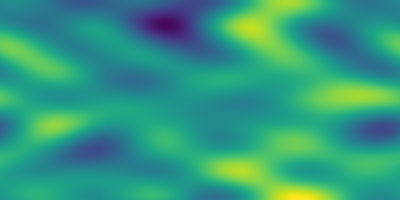
\includegraphics[interpolate=false,width=1.000000in,height=1.000000in]{burgers_rollout_lssvr_pred_0.01-img0.png}}%
\end{pgfscope}%
\begin{pgfscope}%
\pgfsetbuttcap%
\pgfsetroundjoin%
\definecolor{currentfill}{rgb}{0.000000,0.000000,0.000000}%
\pgfsetfillcolor{currentfill}%
\pgfsetlinewidth{0.803000pt}%
\definecolor{currentstroke}{rgb}{0.000000,0.000000,0.000000}%
\pgfsetstrokecolor{currentstroke}%
\pgfsetdash{}{0pt}%
\pgfsys@defobject{currentmarker}{\pgfqpoint{0.000000in}{-0.048611in}}{\pgfqpoint{0.000000in}{0.000000in}}{%
\pgfpathmoveto{\pgfqpoint{0.000000in}{0.000000in}}%
\pgfpathlineto{\pgfqpoint{0.000000in}{-0.048611in}}%
\pgfusepath{stroke,fill}%
}%
\begin{pgfscope}%
\pgfsys@transformshift{0.726837in}{0.517039in}%
\pgfsys@useobject{currentmarker}{}%
\end{pgfscope}%
\end{pgfscope}%
\begin{pgfscope}%
\definecolor{textcolor}{rgb}{0.000000,0.000000,0.000000}%
\pgfsetstrokecolor{textcolor}%
\pgfsetfillcolor{textcolor}%
\pgftext[x=0.726837in,y=0.419816in,,top]{\color{textcolor}\rmfamily\fontsize{12.000000}{14.400000}\selectfont 0}%
\end{pgfscope}%
\begin{pgfscope}%
\pgfsetbuttcap%
\pgfsetroundjoin%
\definecolor{currentfill}{rgb}{0.000000,0.000000,0.000000}%
\pgfsetfillcolor{currentfill}%
\pgfsetlinewidth{0.803000pt}%
\definecolor{currentstroke}{rgb}{0.000000,0.000000,0.000000}%
\pgfsetstrokecolor{currentstroke}%
\pgfsetdash{}{0pt}%
\pgfsys@defobject{currentmarker}{\pgfqpoint{0.000000in}{-0.048611in}}{\pgfqpoint{0.000000in}{0.000000in}}{%
\pgfpathmoveto{\pgfqpoint{0.000000in}{0.000000in}}%
\pgfpathlineto{\pgfqpoint{0.000000in}{-0.048611in}}%
\pgfusepath{stroke,fill}%
}%
\begin{pgfscope}%
\pgfsys@transformshift{1.495432in}{0.517039in}%
\pgfsys@useobject{currentmarker}{}%
\end{pgfscope}%
\end{pgfscope}%
\begin{pgfscope}%
\definecolor{textcolor}{rgb}{0.000000,0.000000,0.000000}%
\pgfsetstrokecolor{textcolor}%
\pgfsetfillcolor{textcolor}%
\pgftext[x=1.495432in,y=0.419816in,,top]{\color{textcolor}\rmfamily\fontsize{12.000000}{14.400000}\selectfont 1}%
\end{pgfscope}%
\begin{pgfscope}%
\pgfsetbuttcap%
\pgfsetroundjoin%
\definecolor{currentfill}{rgb}{0.000000,0.000000,0.000000}%
\pgfsetfillcolor{currentfill}%
\pgfsetlinewidth{0.803000pt}%
\definecolor{currentstroke}{rgb}{0.000000,0.000000,0.000000}%
\pgfsetstrokecolor{currentstroke}%
\pgfsetdash{}{0pt}%
\pgfsys@defobject{currentmarker}{\pgfqpoint{0.000000in}{-0.048611in}}{\pgfqpoint{0.000000in}{0.000000in}}{%
\pgfpathmoveto{\pgfqpoint{0.000000in}{0.000000in}}%
\pgfpathlineto{\pgfqpoint{0.000000in}{-0.048611in}}%
\pgfusepath{stroke,fill}%
}%
\begin{pgfscope}%
\pgfsys@transformshift{2.264026in}{0.517039in}%
\pgfsys@useobject{currentmarker}{}%
\end{pgfscope}%
\end{pgfscope}%
\begin{pgfscope}%
\definecolor{textcolor}{rgb}{0.000000,0.000000,0.000000}%
\pgfsetstrokecolor{textcolor}%
\pgfsetfillcolor{textcolor}%
\pgftext[x=2.264026in,y=0.419816in,,top]{\color{textcolor}\rmfamily\fontsize{12.000000}{14.400000}\selectfont 2}%
\end{pgfscope}%
\begin{pgfscope}%
\definecolor{textcolor}{rgb}{0.000000,0.000000,0.000000}%
\pgfsetstrokecolor{textcolor}%
\pgfsetfillcolor{textcolor}%
\pgftext[x=1.495432in,y=0.202965in,,top]{\color{textcolor}\rmfamily\fontsize{12.000000}{14.400000}\selectfont Space}%
\end{pgfscope}%
\begin{pgfscope}%
\pgfsetbuttcap%
\pgfsetroundjoin%
\definecolor{currentfill}{rgb}{0.000000,0.000000,0.000000}%
\pgfsetfillcolor{currentfill}%
\pgfsetlinewidth{0.803000pt}%
\definecolor{currentstroke}{rgb}{0.000000,0.000000,0.000000}%
\pgfsetstrokecolor{currentstroke}%
\pgfsetdash{}{0pt}%
\pgfsys@defobject{currentmarker}{\pgfqpoint{-0.048611in}{0.000000in}}{\pgfqpoint{-0.000000in}{0.000000in}}{%
\pgfpathmoveto{\pgfqpoint{-0.000000in}{0.000000in}}%
\pgfpathlineto{\pgfqpoint{-0.048611in}{0.000000in}}%
\pgfusepath{stroke,fill}%
}%
\begin{pgfscope}%
\pgfsys@transformshift{0.726837in}{0.517039in}%
\pgfsys@useobject{currentmarker}{}%
\end{pgfscope}%
\end{pgfscope}%
\begin{pgfscope}%
\definecolor{textcolor}{rgb}{0.000000,0.000000,0.000000}%
\pgfsetstrokecolor{textcolor}%
\pgfsetfillcolor{textcolor}%
\pgftext[x=0.364559in, y=0.453725in, left, base]{\color{textcolor}\rmfamily\fontsize{12.000000}{14.400000}\selectfont 0.0}%
\end{pgfscope}%
\begin{pgfscope}%
\pgfsetbuttcap%
\pgfsetroundjoin%
\definecolor{currentfill}{rgb}{0.000000,0.000000,0.000000}%
\pgfsetfillcolor{currentfill}%
\pgfsetlinewidth{0.803000pt}%
\definecolor{currentstroke}{rgb}{0.000000,0.000000,0.000000}%
\pgfsetstrokecolor{currentstroke}%
\pgfsetdash{}{0pt}%
\pgfsys@defobject{currentmarker}{\pgfqpoint{-0.048611in}{0.000000in}}{\pgfqpoint{-0.000000in}{0.000000in}}{%
\pgfpathmoveto{\pgfqpoint{-0.000000in}{0.000000in}}%
\pgfpathlineto{\pgfqpoint{-0.048611in}{0.000000in}}%
\pgfusepath{stroke,fill}%
}%
\begin{pgfscope}%
\pgfsys@transformshift{0.726837in}{0.861533in}%
\pgfsys@useobject{currentmarker}{}%
\end{pgfscope}%
\end{pgfscope}%
\begin{pgfscope}%
\definecolor{textcolor}{rgb}{0.000000,0.000000,0.000000}%
\pgfsetstrokecolor{textcolor}%
\pgfsetfillcolor{textcolor}%
\pgftext[x=0.364559in, y=0.798219in, left, base]{\color{textcolor}\rmfamily\fontsize{12.000000}{14.400000}\selectfont 2.5}%
\end{pgfscope}%
\begin{pgfscope}%
\pgfsetbuttcap%
\pgfsetroundjoin%
\definecolor{currentfill}{rgb}{0.000000,0.000000,0.000000}%
\pgfsetfillcolor{currentfill}%
\pgfsetlinewidth{0.803000pt}%
\definecolor{currentstroke}{rgb}{0.000000,0.000000,0.000000}%
\pgfsetstrokecolor{currentstroke}%
\pgfsetdash{}{0pt}%
\pgfsys@defobject{currentmarker}{\pgfqpoint{-0.048611in}{0.000000in}}{\pgfqpoint{-0.000000in}{0.000000in}}{%
\pgfpathmoveto{\pgfqpoint{-0.000000in}{0.000000in}}%
\pgfpathlineto{\pgfqpoint{-0.048611in}{0.000000in}}%
\pgfusepath{stroke,fill}%
}%
\begin{pgfscope}%
\pgfsys@transformshift{0.726837in}{1.206027in}%
\pgfsys@useobject{currentmarker}{}%
\end{pgfscope}%
\end{pgfscope}%
\begin{pgfscope}%
\definecolor{textcolor}{rgb}{0.000000,0.000000,0.000000}%
\pgfsetstrokecolor{textcolor}%
\pgfsetfillcolor{textcolor}%
\pgftext[x=0.364559in, y=1.142714in, left, base]{\color{textcolor}\rmfamily\fontsize{12.000000}{14.400000}\selectfont 5.0}%
\end{pgfscope}%
\begin{pgfscope}%
\pgfsetbuttcap%
\pgfsetroundjoin%
\definecolor{currentfill}{rgb}{0.000000,0.000000,0.000000}%
\pgfsetfillcolor{currentfill}%
\pgfsetlinewidth{0.803000pt}%
\definecolor{currentstroke}{rgb}{0.000000,0.000000,0.000000}%
\pgfsetstrokecolor{currentstroke}%
\pgfsetdash{}{0pt}%
\pgfsys@defobject{currentmarker}{\pgfqpoint{-0.048611in}{0.000000in}}{\pgfqpoint{-0.000000in}{0.000000in}}{%
\pgfpathmoveto{\pgfqpoint{-0.000000in}{0.000000in}}%
\pgfpathlineto{\pgfqpoint{-0.048611in}{0.000000in}}%
\pgfusepath{stroke,fill}%
}%
\begin{pgfscope}%
\pgfsys@transformshift{0.726837in}{1.550522in}%
\pgfsys@useobject{currentmarker}{}%
\end{pgfscope}%
\end{pgfscope}%
\begin{pgfscope}%
\definecolor{textcolor}{rgb}{0.000000,0.000000,0.000000}%
\pgfsetstrokecolor{textcolor}%
\pgfsetfillcolor{textcolor}%
\pgftext[x=0.364559in, y=1.487208in, left, base]{\color{textcolor}\rmfamily\fontsize{12.000000}{14.400000}\selectfont 7.5}%
\end{pgfscope}%
\begin{pgfscope}%
\pgfsetbuttcap%
\pgfsetroundjoin%
\definecolor{currentfill}{rgb}{0.000000,0.000000,0.000000}%
\pgfsetfillcolor{currentfill}%
\pgfsetlinewidth{0.803000pt}%
\definecolor{currentstroke}{rgb}{0.000000,0.000000,0.000000}%
\pgfsetstrokecolor{currentstroke}%
\pgfsetdash{}{0pt}%
\pgfsys@defobject{currentmarker}{\pgfqpoint{-0.048611in}{0.000000in}}{\pgfqpoint{-0.000000in}{0.000000in}}{%
\pgfpathmoveto{\pgfqpoint{-0.000000in}{0.000000in}}%
\pgfpathlineto{\pgfqpoint{-0.048611in}{0.000000in}}%
\pgfusepath{stroke,fill}%
}%
\begin{pgfscope}%
\pgfsys@transformshift{0.726837in}{1.895016in}%
\pgfsys@useobject{currentmarker}{}%
\end{pgfscope}%
\end{pgfscope}%
\begin{pgfscope}%
\definecolor{textcolor}{rgb}{0.000000,0.000000,0.000000}%
\pgfsetstrokecolor{textcolor}%
\pgfsetfillcolor{textcolor}%
\pgftext[x=0.258521in, y=1.831702in, left, base]{\color{textcolor}\rmfamily\fontsize{12.000000}{14.400000}\selectfont 10.0}%
\end{pgfscope}%
\begin{pgfscope}%
\definecolor{textcolor}{rgb}{0.000000,0.000000,0.000000}%
\pgfsetstrokecolor{textcolor}%
\pgfsetfillcolor{textcolor}%
\pgftext[x=0.202965in,y=1.206027in,,bottom,rotate=90.000000]{\color{textcolor}\rmfamily\fontsize{12.000000}{14.400000}\selectfont Time}%
\end{pgfscope}%
\begin{pgfscope}%
\pgfsetrectcap%
\pgfsetmiterjoin%
\pgfsetlinewidth{0.803000pt}%
\definecolor{currentstroke}{rgb}{0.000000,0.000000,0.000000}%
\pgfsetstrokecolor{currentstroke}%
\pgfsetdash{}{0pt}%
\pgfpathmoveto{\pgfqpoint{0.726837in}{0.517039in}}%
\pgfpathlineto{\pgfqpoint{0.726837in}{1.895016in}}%
\pgfusepath{stroke}%
\end{pgfscope}%
\begin{pgfscope}%
\pgfsetrectcap%
\pgfsetmiterjoin%
\pgfsetlinewidth{0.803000pt}%
\definecolor{currentstroke}{rgb}{0.000000,0.000000,0.000000}%
\pgfsetstrokecolor{currentstroke}%
\pgfsetdash{}{0pt}%
\pgfpathmoveto{\pgfqpoint{2.264026in}{0.517039in}}%
\pgfpathlineto{\pgfqpoint{2.264026in}{1.895016in}}%
\pgfusepath{stroke}%
\end{pgfscope}%
\begin{pgfscope}%
\pgfsetrectcap%
\pgfsetmiterjoin%
\pgfsetlinewidth{0.803000pt}%
\definecolor{currentstroke}{rgb}{0.000000,0.000000,0.000000}%
\pgfsetstrokecolor{currentstroke}%
\pgfsetdash{}{0pt}%
\pgfpathmoveto{\pgfqpoint{0.726837in}{0.517039in}}%
\pgfpathlineto{\pgfqpoint{2.264026in}{0.517039in}}%
\pgfusepath{stroke}%
\end{pgfscope}%
\begin{pgfscope}%
\pgfsetrectcap%
\pgfsetmiterjoin%
\pgfsetlinewidth{0.803000pt}%
\definecolor{currentstroke}{rgb}{0.000000,0.000000,0.000000}%
\pgfsetstrokecolor{currentstroke}%
\pgfsetdash{}{0pt}%
\pgfpathmoveto{\pgfqpoint{0.726837in}{1.895016in}}%
\pgfpathlineto{\pgfqpoint{2.264026in}{1.895016in}}%
\pgfusepath{stroke}%
\end{pgfscope}%
\begin{pgfscope}%
\pgfsetbuttcap%
\pgfsetmiterjoin%
\pgfsetlinewidth{0.000000pt}%
\definecolor{currentstroke}{rgb}{0.000000,0.000000,0.000000}%
\pgfsetstrokecolor{currentstroke}%
\pgfsetstrokeopacity{0.000000}%
\pgfsetdash{}{0pt}%
\pgfpathmoveto{\pgfqpoint{2.393905in}{0.517039in}}%
\pgfpathlineto{\pgfqpoint{2.462804in}{0.517039in}}%
\pgfpathlineto{\pgfqpoint{2.462804in}{1.895016in}}%
\pgfpathlineto{\pgfqpoint{2.393905in}{1.895016in}}%
\pgfpathlineto{\pgfqpoint{2.393905in}{0.517039in}}%
\pgfpathclose%
\pgfusepath{}%
\end{pgfscope}%
\begin{pgfscope}%
\pgfsys@transformshift{2.390000in}{0.520000in}%
\pgftext[left,bottom]{
\includegraphics[interpolate=true,width=0.070000in,height=1.380000in]{burgers_rollout_lssvr_pred_0.01-img1.png}}%
\end{pgfscope}%
\begin{pgfscope}%
\pgfsetbuttcap%
\pgfsetroundjoin%
\definecolor{currentfill}{rgb}{0.000000,0.000000,0.000000}%
\pgfsetfillcolor{currentfill}%
\pgfsetlinewidth{0.803000pt}%
\definecolor{currentstroke}{rgb}{0.000000,0.000000,0.000000}%
\pgfsetstrokecolor{currentstroke}%
\pgfsetdash{}{0pt}%
\pgfsys@defobject{currentmarker}{\pgfqpoint{0.000000in}{0.000000in}}{\pgfqpoint{0.048611in}{0.000000in}}{%
\pgfpathmoveto{\pgfqpoint{0.000000in}{0.000000in}}%
\pgfpathlineto{\pgfqpoint{0.048611in}{0.000000in}}%
\pgfusepath{stroke,fill}%
}%
\begin{pgfscope}%
\pgfsys@transformshift{2.462804in}{0.839076in}%
\pgfsys@useobject{currentmarker}{}%
\end{pgfscope}%
\end{pgfscope}%
\begin{pgfscope}%
\definecolor{textcolor}{rgb}{0.000000,0.000000,0.000000}%
\pgfsetstrokecolor{textcolor}%
\pgfsetfillcolor{textcolor}%
\pgftext[x=2.560026in, y=0.775762in, left, base]{\color{textcolor}\rmfamily\fontsize{12.000000}{14.400000}\selectfont \ensuremath{-}0.5}%
\end{pgfscope}%
\begin{pgfscope}%
\pgfsetbuttcap%
\pgfsetroundjoin%
\definecolor{currentfill}{rgb}{0.000000,0.000000,0.000000}%
\pgfsetfillcolor{currentfill}%
\pgfsetlinewidth{0.803000pt}%
\definecolor{currentstroke}{rgb}{0.000000,0.000000,0.000000}%
\pgfsetstrokecolor{currentstroke}%
\pgfsetdash{}{0pt}%
\pgfsys@defobject{currentmarker}{\pgfqpoint{0.000000in}{0.000000in}}{\pgfqpoint{0.048611in}{0.000000in}}{%
\pgfpathmoveto{\pgfqpoint{0.000000in}{0.000000in}}%
\pgfpathlineto{\pgfqpoint{0.048611in}{0.000000in}}%
\pgfusepath{stroke,fill}%
}%
\begin{pgfscope}%
\pgfsys@transformshift{2.462804in}{1.206027in}%
\pgfsys@useobject{currentmarker}{}%
\end{pgfscope}%
\end{pgfscope}%
\begin{pgfscope}%
\definecolor{textcolor}{rgb}{0.000000,0.000000,0.000000}%
\pgfsetstrokecolor{textcolor}%
\pgfsetfillcolor{textcolor}%
\pgftext[x=2.560026in, y=1.142714in, left, base]{\color{textcolor}\rmfamily\fontsize{12.000000}{14.400000}\selectfont 0.0}%
\end{pgfscope}%
\begin{pgfscope}%
\pgfsetbuttcap%
\pgfsetroundjoin%
\definecolor{currentfill}{rgb}{0.000000,0.000000,0.000000}%
\pgfsetfillcolor{currentfill}%
\pgfsetlinewidth{0.803000pt}%
\definecolor{currentstroke}{rgb}{0.000000,0.000000,0.000000}%
\pgfsetstrokecolor{currentstroke}%
\pgfsetdash{}{0pt}%
\pgfsys@defobject{currentmarker}{\pgfqpoint{0.000000in}{0.000000in}}{\pgfqpoint{0.048611in}{0.000000in}}{%
\pgfpathmoveto{\pgfqpoint{0.000000in}{0.000000in}}%
\pgfpathlineto{\pgfqpoint{0.048611in}{0.000000in}}%
\pgfusepath{stroke,fill}%
}%
\begin{pgfscope}%
\pgfsys@transformshift{2.462804in}{1.572979in}%
\pgfsys@useobject{currentmarker}{}%
\end{pgfscope}%
\end{pgfscope}%
\begin{pgfscope}%
\definecolor{textcolor}{rgb}{0.000000,0.000000,0.000000}%
\pgfsetstrokecolor{textcolor}%
\pgfsetfillcolor{textcolor}%
\pgftext[x=2.560026in, y=1.509665in, left, base]{\color{textcolor}\rmfamily\fontsize{12.000000}{14.400000}\selectfont 0.5}%
\end{pgfscope}%
\begin{pgfscope}%
\pgfsetrectcap%
\pgfsetmiterjoin%
\pgfsetlinewidth{0.803000pt}%
\definecolor{currentstroke}{rgb}{0.000000,0.000000,0.000000}%
\pgfsetstrokecolor{currentstroke}%
\pgfsetdash{}{0pt}%
\pgfpathmoveto{\pgfqpoint{2.393905in}{0.517039in}}%
\pgfpathlineto{\pgfqpoint{2.428354in}{0.517039in}}%
\pgfpathlineto{\pgfqpoint{2.462804in}{0.517039in}}%
\pgfpathlineto{\pgfqpoint{2.462804in}{1.895016in}}%
\pgfpathlineto{\pgfqpoint{2.428354in}{1.895016in}}%
\pgfpathlineto{\pgfqpoint{2.393905in}{1.895016in}}%
\pgfpathlineto{\pgfqpoint{2.393905in}{0.517039in}}%
\pgfpathclose%
\pgfusepath{stroke}%
\end{pgfscope}%
\end{pgfpicture}%
\makeatother%
\endgroup%

      \end{adjustbox}
      \caption{SpectralSVR prediction.}\label{fig:comp_lssvr_pred_0.01}
    \end{subfigure}
    \begin{subfigure}{0.49\linewidth}
      \begin{adjustbox}{width=\linewidth}
        \begingroup%
\makeatletter%
\begin{pgfpicture}%
\pgfpathrectangle{\pgfpointorigin}{\pgfqpoint{3.000000in}{2.000000in}}%
\pgfusepath{use as bounding box, clip}%
\begin{pgfscope}%
\pgfsetbuttcap%
\pgfsetmiterjoin%
\pgfsetlinewidth{0.000000pt}%
\definecolor{currentstroke}{rgb}{0.000000,0.000000,0.000000}%
\pgfsetstrokecolor{currentstroke}%
\pgfsetstrokeopacity{0.000000}%
\pgfsetdash{}{0pt}%
\pgfpathmoveto{\pgfqpoint{0.000000in}{0.000000in}}%
\pgfpathlineto{\pgfqpoint{3.000000in}{0.000000in}}%
\pgfpathlineto{\pgfqpoint{3.000000in}{2.000000in}}%
\pgfpathlineto{\pgfqpoint{0.000000in}{2.000000in}}%
\pgfpathlineto{\pgfqpoint{0.000000in}{0.000000in}}%
\pgfpathclose%
\pgfusepath{}%
\end{pgfscope}%
\begin{pgfscope}%
\pgfsetbuttcap%
\pgfsetmiterjoin%
\pgfsetlinewidth{0.000000pt}%
\definecolor{currentstroke}{rgb}{0.000000,0.000000,0.000000}%
\pgfsetstrokecolor{currentstroke}%
\pgfsetstrokeopacity{0.000000}%
\pgfsetdash{}{0pt}%
\pgfpathmoveto{\pgfqpoint{0.726837in}{0.517039in}}%
\pgfpathlineto{\pgfqpoint{2.264026in}{0.517039in}}%
\pgfpathlineto{\pgfqpoint{2.264026in}{1.895016in}}%
\pgfpathlineto{\pgfqpoint{0.726837in}{1.895016in}}%
\pgfpathlineto{\pgfqpoint{0.726837in}{0.517039in}}%
\pgfpathclose%
\pgfusepath{}%
\end{pgfscope}%
\begin{pgfscope}%
\pgfpathrectangle{\pgfqpoint{0.726837in}{0.517039in}}{\pgfqpoint{1.537189in}{1.377978in}}%
\pgfusepath{clip}%
\pgfsys@transformcm{1.537189}{0.000000}{0.000000}{1.377978}{0.726837in}{0.517039in}%
\pgftext[left,bottom]{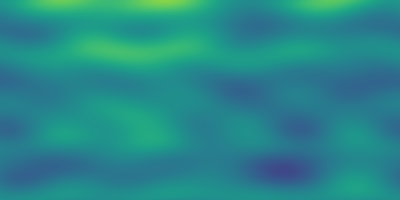
\includegraphics[interpolate=false,width=1.000000in,height=1.000000in]{burgers_rollout_lssvr_diff_0.01-img0.png}}%
\end{pgfscope}%
\begin{pgfscope}%
\pgfsetbuttcap%
\pgfsetroundjoin%
\definecolor{currentfill}{rgb}{0.000000,0.000000,0.000000}%
\pgfsetfillcolor{currentfill}%
\pgfsetlinewidth{0.803000pt}%
\definecolor{currentstroke}{rgb}{0.000000,0.000000,0.000000}%
\pgfsetstrokecolor{currentstroke}%
\pgfsetdash{}{0pt}%
\pgfsys@defobject{currentmarker}{\pgfqpoint{0.000000in}{-0.048611in}}{\pgfqpoint{0.000000in}{0.000000in}}{%
\pgfpathmoveto{\pgfqpoint{0.000000in}{0.000000in}}%
\pgfpathlineto{\pgfqpoint{0.000000in}{-0.048611in}}%
\pgfusepath{stroke,fill}%
}%
\begin{pgfscope}%
\pgfsys@transformshift{0.726837in}{0.517039in}%
\pgfsys@useobject{currentmarker}{}%
\end{pgfscope}%
\end{pgfscope}%
\begin{pgfscope}%
\definecolor{textcolor}{rgb}{0.000000,0.000000,0.000000}%
\pgfsetstrokecolor{textcolor}%
\pgfsetfillcolor{textcolor}%
\pgftext[x=0.726837in,y=0.419816in,,top]{\color{textcolor}\rmfamily\fontsize{12.000000}{14.400000}\selectfont 0}%
\end{pgfscope}%
\begin{pgfscope}%
\pgfsetbuttcap%
\pgfsetroundjoin%
\definecolor{currentfill}{rgb}{0.000000,0.000000,0.000000}%
\pgfsetfillcolor{currentfill}%
\pgfsetlinewidth{0.803000pt}%
\definecolor{currentstroke}{rgb}{0.000000,0.000000,0.000000}%
\pgfsetstrokecolor{currentstroke}%
\pgfsetdash{}{0pt}%
\pgfsys@defobject{currentmarker}{\pgfqpoint{0.000000in}{-0.048611in}}{\pgfqpoint{0.000000in}{0.000000in}}{%
\pgfpathmoveto{\pgfqpoint{0.000000in}{0.000000in}}%
\pgfpathlineto{\pgfqpoint{0.000000in}{-0.048611in}}%
\pgfusepath{stroke,fill}%
}%
\begin{pgfscope}%
\pgfsys@transformshift{1.495432in}{0.517039in}%
\pgfsys@useobject{currentmarker}{}%
\end{pgfscope}%
\end{pgfscope}%
\begin{pgfscope}%
\definecolor{textcolor}{rgb}{0.000000,0.000000,0.000000}%
\pgfsetstrokecolor{textcolor}%
\pgfsetfillcolor{textcolor}%
\pgftext[x=1.495432in,y=0.419816in,,top]{\color{textcolor}\rmfamily\fontsize{12.000000}{14.400000}\selectfont 1}%
\end{pgfscope}%
\begin{pgfscope}%
\pgfsetbuttcap%
\pgfsetroundjoin%
\definecolor{currentfill}{rgb}{0.000000,0.000000,0.000000}%
\pgfsetfillcolor{currentfill}%
\pgfsetlinewidth{0.803000pt}%
\definecolor{currentstroke}{rgb}{0.000000,0.000000,0.000000}%
\pgfsetstrokecolor{currentstroke}%
\pgfsetdash{}{0pt}%
\pgfsys@defobject{currentmarker}{\pgfqpoint{0.000000in}{-0.048611in}}{\pgfqpoint{0.000000in}{0.000000in}}{%
\pgfpathmoveto{\pgfqpoint{0.000000in}{0.000000in}}%
\pgfpathlineto{\pgfqpoint{0.000000in}{-0.048611in}}%
\pgfusepath{stroke,fill}%
}%
\begin{pgfscope}%
\pgfsys@transformshift{2.264026in}{0.517039in}%
\pgfsys@useobject{currentmarker}{}%
\end{pgfscope}%
\end{pgfscope}%
\begin{pgfscope}%
\definecolor{textcolor}{rgb}{0.000000,0.000000,0.000000}%
\pgfsetstrokecolor{textcolor}%
\pgfsetfillcolor{textcolor}%
\pgftext[x=2.264026in,y=0.419816in,,top]{\color{textcolor}\rmfamily\fontsize{12.000000}{14.400000}\selectfont 2}%
\end{pgfscope}%
\begin{pgfscope}%
\definecolor{textcolor}{rgb}{0.000000,0.000000,0.000000}%
\pgfsetstrokecolor{textcolor}%
\pgfsetfillcolor{textcolor}%
\pgftext[x=1.495432in,y=0.202965in,,top]{\color{textcolor}\rmfamily\fontsize{12.000000}{14.400000}\selectfont Space}%
\end{pgfscope}%
\begin{pgfscope}%
\pgfsetbuttcap%
\pgfsetroundjoin%
\definecolor{currentfill}{rgb}{0.000000,0.000000,0.000000}%
\pgfsetfillcolor{currentfill}%
\pgfsetlinewidth{0.803000pt}%
\definecolor{currentstroke}{rgb}{0.000000,0.000000,0.000000}%
\pgfsetstrokecolor{currentstroke}%
\pgfsetdash{}{0pt}%
\pgfsys@defobject{currentmarker}{\pgfqpoint{-0.048611in}{0.000000in}}{\pgfqpoint{-0.000000in}{0.000000in}}{%
\pgfpathmoveto{\pgfqpoint{-0.000000in}{0.000000in}}%
\pgfpathlineto{\pgfqpoint{-0.048611in}{0.000000in}}%
\pgfusepath{stroke,fill}%
}%
\begin{pgfscope}%
\pgfsys@transformshift{0.726837in}{0.517039in}%
\pgfsys@useobject{currentmarker}{}%
\end{pgfscope}%
\end{pgfscope}%
\begin{pgfscope}%
\definecolor{textcolor}{rgb}{0.000000,0.000000,0.000000}%
\pgfsetstrokecolor{textcolor}%
\pgfsetfillcolor{textcolor}%
\pgftext[x=0.364559in, y=0.453725in, left, base]{\color{textcolor}\rmfamily\fontsize{12.000000}{14.400000}\selectfont 0.0}%
\end{pgfscope}%
\begin{pgfscope}%
\pgfsetbuttcap%
\pgfsetroundjoin%
\definecolor{currentfill}{rgb}{0.000000,0.000000,0.000000}%
\pgfsetfillcolor{currentfill}%
\pgfsetlinewidth{0.803000pt}%
\definecolor{currentstroke}{rgb}{0.000000,0.000000,0.000000}%
\pgfsetstrokecolor{currentstroke}%
\pgfsetdash{}{0pt}%
\pgfsys@defobject{currentmarker}{\pgfqpoint{-0.048611in}{0.000000in}}{\pgfqpoint{-0.000000in}{0.000000in}}{%
\pgfpathmoveto{\pgfqpoint{-0.000000in}{0.000000in}}%
\pgfpathlineto{\pgfqpoint{-0.048611in}{0.000000in}}%
\pgfusepath{stroke,fill}%
}%
\begin{pgfscope}%
\pgfsys@transformshift{0.726837in}{0.861533in}%
\pgfsys@useobject{currentmarker}{}%
\end{pgfscope}%
\end{pgfscope}%
\begin{pgfscope}%
\definecolor{textcolor}{rgb}{0.000000,0.000000,0.000000}%
\pgfsetstrokecolor{textcolor}%
\pgfsetfillcolor{textcolor}%
\pgftext[x=0.364559in, y=0.798219in, left, base]{\color{textcolor}\rmfamily\fontsize{12.000000}{14.400000}\selectfont 2.5}%
\end{pgfscope}%
\begin{pgfscope}%
\pgfsetbuttcap%
\pgfsetroundjoin%
\definecolor{currentfill}{rgb}{0.000000,0.000000,0.000000}%
\pgfsetfillcolor{currentfill}%
\pgfsetlinewidth{0.803000pt}%
\definecolor{currentstroke}{rgb}{0.000000,0.000000,0.000000}%
\pgfsetstrokecolor{currentstroke}%
\pgfsetdash{}{0pt}%
\pgfsys@defobject{currentmarker}{\pgfqpoint{-0.048611in}{0.000000in}}{\pgfqpoint{-0.000000in}{0.000000in}}{%
\pgfpathmoveto{\pgfqpoint{-0.000000in}{0.000000in}}%
\pgfpathlineto{\pgfqpoint{-0.048611in}{0.000000in}}%
\pgfusepath{stroke,fill}%
}%
\begin{pgfscope}%
\pgfsys@transformshift{0.726837in}{1.206027in}%
\pgfsys@useobject{currentmarker}{}%
\end{pgfscope}%
\end{pgfscope}%
\begin{pgfscope}%
\definecolor{textcolor}{rgb}{0.000000,0.000000,0.000000}%
\pgfsetstrokecolor{textcolor}%
\pgfsetfillcolor{textcolor}%
\pgftext[x=0.364559in, y=1.142714in, left, base]{\color{textcolor}\rmfamily\fontsize{12.000000}{14.400000}\selectfont 5.0}%
\end{pgfscope}%
\begin{pgfscope}%
\pgfsetbuttcap%
\pgfsetroundjoin%
\definecolor{currentfill}{rgb}{0.000000,0.000000,0.000000}%
\pgfsetfillcolor{currentfill}%
\pgfsetlinewidth{0.803000pt}%
\definecolor{currentstroke}{rgb}{0.000000,0.000000,0.000000}%
\pgfsetstrokecolor{currentstroke}%
\pgfsetdash{}{0pt}%
\pgfsys@defobject{currentmarker}{\pgfqpoint{-0.048611in}{0.000000in}}{\pgfqpoint{-0.000000in}{0.000000in}}{%
\pgfpathmoveto{\pgfqpoint{-0.000000in}{0.000000in}}%
\pgfpathlineto{\pgfqpoint{-0.048611in}{0.000000in}}%
\pgfusepath{stroke,fill}%
}%
\begin{pgfscope}%
\pgfsys@transformshift{0.726837in}{1.550522in}%
\pgfsys@useobject{currentmarker}{}%
\end{pgfscope}%
\end{pgfscope}%
\begin{pgfscope}%
\definecolor{textcolor}{rgb}{0.000000,0.000000,0.000000}%
\pgfsetstrokecolor{textcolor}%
\pgfsetfillcolor{textcolor}%
\pgftext[x=0.364559in, y=1.487208in, left, base]{\color{textcolor}\rmfamily\fontsize{12.000000}{14.400000}\selectfont 7.5}%
\end{pgfscope}%
\begin{pgfscope}%
\pgfsetbuttcap%
\pgfsetroundjoin%
\definecolor{currentfill}{rgb}{0.000000,0.000000,0.000000}%
\pgfsetfillcolor{currentfill}%
\pgfsetlinewidth{0.803000pt}%
\definecolor{currentstroke}{rgb}{0.000000,0.000000,0.000000}%
\pgfsetstrokecolor{currentstroke}%
\pgfsetdash{}{0pt}%
\pgfsys@defobject{currentmarker}{\pgfqpoint{-0.048611in}{0.000000in}}{\pgfqpoint{-0.000000in}{0.000000in}}{%
\pgfpathmoveto{\pgfqpoint{-0.000000in}{0.000000in}}%
\pgfpathlineto{\pgfqpoint{-0.048611in}{0.000000in}}%
\pgfusepath{stroke,fill}%
}%
\begin{pgfscope}%
\pgfsys@transformshift{0.726837in}{1.895016in}%
\pgfsys@useobject{currentmarker}{}%
\end{pgfscope}%
\end{pgfscope}%
\begin{pgfscope}%
\definecolor{textcolor}{rgb}{0.000000,0.000000,0.000000}%
\pgfsetstrokecolor{textcolor}%
\pgfsetfillcolor{textcolor}%
\pgftext[x=0.258521in, y=1.831702in, left, base]{\color{textcolor}\rmfamily\fontsize{12.000000}{14.400000}\selectfont 10.0}%
\end{pgfscope}%
\begin{pgfscope}%
\definecolor{textcolor}{rgb}{0.000000,0.000000,0.000000}%
\pgfsetstrokecolor{textcolor}%
\pgfsetfillcolor{textcolor}%
\pgftext[x=0.202965in,y=1.206027in,,bottom,rotate=90.000000]{\color{textcolor}\rmfamily\fontsize{12.000000}{14.400000}\selectfont Time}%
\end{pgfscope}%
\begin{pgfscope}%
\pgfsetrectcap%
\pgfsetmiterjoin%
\pgfsetlinewidth{0.803000pt}%
\definecolor{currentstroke}{rgb}{0.000000,0.000000,0.000000}%
\pgfsetstrokecolor{currentstroke}%
\pgfsetdash{}{0pt}%
\pgfpathmoveto{\pgfqpoint{0.726837in}{0.517039in}}%
\pgfpathlineto{\pgfqpoint{0.726837in}{1.895016in}}%
\pgfusepath{stroke}%
\end{pgfscope}%
\begin{pgfscope}%
\pgfsetrectcap%
\pgfsetmiterjoin%
\pgfsetlinewidth{0.803000pt}%
\definecolor{currentstroke}{rgb}{0.000000,0.000000,0.000000}%
\pgfsetstrokecolor{currentstroke}%
\pgfsetdash{}{0pt}%
\pgfpathmoveto{\pgfqpoint{2.264026in}{0.517039in}}%
\pgfpathlineto{\pgfqpoint{2.264026in}{1.895016in}}%
\pgfusepath{stroke}%
\end{pgfscope}%
\begin{pgfscope}%
\pgfsetrectcap%
\pgfsetmiterjoin%
\pgfsetlinewidth{0.803000pt}%
\definecolor{currentstroke}{rgb}{0.000000,0.000000,0.000000}%
\pgfsetstrokecolor{currentstroke}%
\pgfsetdash{}{0pt}%
\pgfpathmoveto{\pgfqpoint{0.726837in}{0.517039in}}%
\pgfpathlineto{\pgfqpoint{2.264026in}{0.517039in}}%
\pgfusepath{stroke}%
\end{pgfscope}%
\begin{pgfscope}%
\pgfsetrectcap%
\pgfsetmiterjoin%
\pgfsetlinewidth{0.803000pt}%
\definecolor{currentstroke}{rgb}{0.000000,0.000000,0.000000}%
\pgfsetstrokecolor{currentstroke}%
\pgfsetdash{}{0pt}%
\pgfpathmoveto{\pgfqpoint{0.726837in}{1.895016in}}%
\pgfpathlineto{\pgfqpoint{2.264026in}{1.895016in}}%
\pgfusepath{stroke}%
\end{pgfscope}%
\begin{pgfscope}%
\pgfsetbuttcap%
\pgfsetmiterjoin%
\pgfsetlinewidth{0.000000pt}%
\definecolor{currentstroke}{rgb}{0.000000,0.000000,0.000000}%
\pgfsetstrokecolor{currentstroke}%
\pgfsetstrokeopacity{0.000000}%
\pgfsetdash{}{0pt}%
\pgfpathmoveto{\pgfqpoint{2.393905in}{0.517039in}}%
\pgfpathlineto{\pgfqpoint{2.462804in}{0.517039in}}%
\pgfpathlineto{\pgfqpoint{2.462804in}{1.895016in}}%
\pgfpathlineto{\pgfqpoint{2.393905in}{1.895016in}}%
\pgfpathlineto{\pgfqpoint{2.393905in}{0.517039in}}%
\pgfpathclose%
\pgfusepath{}%
\end{pgfscope}%
\begin{pgfscope}%
\pgfsys@transformshift{2.390000in}{0.520000in}%
\pgftext[left,bottom]{
\includegraphics[interpolate=true,width=0.070000in,height=1.380000in]{burgers_rollout_lssvr_diff_0.01-img1.png}}%
\end{pgfscope}%
\begin{pgfscope}%
\pgfsetbuttcap%
\pgfsetroundjoin%
\definecolor{currentfill}{rgb}{0.000000,0.000000,0.000000}%
\pgfsetfillcolor{currentfill}%
\pgfsetlinewidth{0.803000pt}%
\definecolor{currentstroke}{rgb}{0.000000,0.000000,0.000000}%
\pgfsetstrokecolor{currentstroke}%
\pgfsetdash{}{0pt}%
\pgfsys@defobject{currentmarker}{\pgfqpoint{0.000000in}{0.000000in}}{\pgfqpoint{0.048611in}{0.000000in}}{%
\pgfpathmoveto{\pgfqpoint{0.000000in}{0.000000in}}%
\pgfpathlineto{\pgfqpoint{0.048611in}{0.000000in}}%
\pgfusepath{stroke,fill}%
}%
\begin{pgfscope}%
\pgfsys@transformshift{2.462804in}{0.839076in}%
\pgfsys@useobject{currentmarker}{}%
\end{pgfscope}%
\end{pgfscope}%
\begin{pgfscope}%
\definecolor{textcolor}{rgb}{0.000000,0.000000,0.000000}%
\pgfsetstrokecolor{textcolor}%
\pgfsetfillcolor{textcolor}%
\pgftext[x=2.560026in, y=0.775762in, left, base]{\color{textcolor}\rmfamily\fontsize{12.000000}{14.400000}\selectfont \ensuremath{-}0.5}%
\end{pgfscope}%
\begin{pgfscope}%
\pgfsetbuttcap%
\pgfsetroundjoin%
\definecolor{currentfill}{rgb}{0.000000,0.000000,0.000000}%
\pgfsetfillcolor{currentfill}%
\pgfsetlinewidth{0.803000pt}%
\definecolor{currentstroke}{rgb}{0.000000,0.000000,0.000000}%
\pgfsetstrokecolor{currentstroke}%
\pgfsetdash{}{0pt}%
\pgfsys@defobject{currentmarker}{\pgfqpoint{0.000000in}{0.000000in}}{\pgfqpoint{0.048611in}{0.000000in}}{%
\pgfpathmoveto{\pgfqpoint{0.000000in}{0.000000in}}%
\pgfpathlineto{\pgfqpoint{0.048611in}{0.000000in}}%
\pgfusepath{stroke,fill}%
}%
\begin{pgfscope}%
\pgfsys@transformshift{2.462804in}{1.206027in}%
\pgfsys@useobject{currentmarker}{}%
\end{pgfscope}%
\end{pgfscope}%
\begin{pgfscope}%
\definecolor{textcolor}{rgb}{0.000000,0.000000,0.000000}%
\pgfsetstrokecolor{textcolor}%
\pgfsetfillcolor{textcolor}%
\pgftext[x=2.560026in, y=1.142714in, left, base]{\color{textcolor}\rmfamily\fontsize{12.000000}{14.400000}\selectfont 0.0}%
\end{pgfscope}%
\begin{pgfscope}%
\pgfsetbuttcap%
\pgfsetroundjoin%
\definecolor{currentfill}{rgb}{0.000000,0.000000,0.000000}%
\pgfsetfillcolor{currentfill}%
\pgfsetlinewidth{0.803000pt}%
\definecolor{currentstroke}{rgb}{0.000000,0.000000,0.000000}%
\pgfsetstrokecolor{currentstroke}%
\pgfsetdash{}{0pt}%
\pgfsys@defobject{currentmarker}{\pgfqpoint{0.000000in}{0.000000in}}{\pgfqpoint{0.048611in}{0.000000in}}{%
\pgfpathmoveto{\pgfqpoint{0.000000in}{0.000000in}}%
\pgfpathlineto{\pgfqpoint{0.048611in}{0.000000in}}%
\pgfusepath{stroke,fill}%
}%
\begin{pgfscope}%
\pgfsys@transformshift{2.462804in}{1.572979in}%
\pgfsys@useobject{currentmarker}{}%
\end{pgfscope}%
\end{pgfscope}%
\begin{pgfscope}%
\definecolor{textcolor}{rgb}{0.000000,0.000000,0.000000}%
\pgfsetstrokecolor{textcolor}%
\pgfsetfillcolor{textcolor}%
\pgftext[x=2.560026in, y=1.509665in, left, base]{\color{textcolor}\rmfamily\fontsize{12.000000}{14.400000}\selectfont 0.5}%
\end{pgfscope}%
\begin{pgfscope}%
\pgfsetrectcap%
\pgfsetmiterjoin%
\pgfsetlinewidth{0.803000pt}%
\definecolor{currentstroke}{rgb}{0.000000,0.000000,0.000000}%
\pgfsetstrokecolor{currentstroke}%
\pgfsetdash{}{0pt}%
\pgfpathmoveto{\pgfqpoint{2.393905in}{0.517039in}}%
\pgfpathlineto{\pgfqpoint{2.428354in}{0.517039in}}%
\pgfpathlineto{\pgfqpoint{2.462804in}{0.517039in}}%
\pgfpathlineto{\pgfqpoint{2.462804in}{1.895016in}}%
\pgfpathlineto{\pgfqpoint{2.428354in}{1.895016in}}%
\pgfpathlineto{\pgfqpoint{2.393905in}{1.895016in}}%
\pgfpathlineto{\pgfqpoint{2.393905in}{0.517039in}}%
\pgfpathclose%
\pgfusepath{stroke}%
\end{pgfscope}%
\end{pgfpicture}%
\makeatother%
\endgroup%

      \end{adjustbox}
      \caption{SpectralSVR difference with target.}\label{fig:comp_lssvr_diff_0.01}
    \end{subfigure}
    \begin{subfigure}{0.49\linewidth}
      \begin{adjustbox}{width=\linewidth}
        \begingroup%
\makeatletter%
\begin{pgfpicture}%
\pgfpathrectangle{\pgfpointorigin}{\pgfqpoint{3.000000in}{2.000000in}}%
\pgfusepath{use as bounding box, clip}%
\begin{pgfscope}%
\pgfsetbuttcap%
\pgfsetmiterjoin%
\pgfsetlinewidth{0.000000pt}%
\definecolor{currentstroke}{rgb}{0.000000,0.000000,0.000000}%
\pgfsetstrokecolor{currentstroke}%
\pgfsetstrokeopacity{0.000000}%
\pgfsetdash{}{0pt}%
\pgfpathmoveto{\pgfqpoint{0.000000in}{0.000000in}}%
\pgfpathlineto{\pgfqpoint{3.000000in}{0.000000in}}%
\pgfpathlineto{\pgfqpoint{3.000000in}{2.000000in}}%
\pgfpathlineto{\pgfqpoint{0.000000in}{2.000000in}}%
\pgfpathlineto{\pgfqpoint{0.000000in}{0.000000in}}%
\pgfpathclose%
\pgfusepath{}%
\end{pgfscope}%
\begin{pgfscope}%
\pgfsetbuttcap%
\pgfsetmiterjoin%
\pgfsetlinewidth{0.000000pt}%
\definecolor{currentstroke}{rgb}{0.000000,0.000000,0.000000}%
\pgfsetstrokecolor{currentstroke}%
\pgfsetstrokeopacity{0.000000}%
\pgfsetdash{}{0pt}%
\pgfpathmoveto{\pgfqpoint{0.726837in}{0.517039in}}%
\pgfpathlineto{\pgfqpoint{2.264026in}{0.517039in}}%
\pgfpathlineto{\pgfqpoint{2.264026in}{1.895016in}}%
\pgfpathlineto{\pgfqpoint{0.726837in}{1.895016in}}%
\pgfpathlineto{\pgfqpoint{0.726837in}{0.517039in}}%
\pgfpathclose%
\pgfusepath{}%
\end{pgfscope}%
\begin{pgfscope}%
\pgfpathrectangle{\pgfqpoint{0.726837in}{0.517039in}}{\pgfqpoint{1.537189in}{1.377978in}}%
\pgfusepath{clip}%
\pgfsys@transformcm{1.537189}{0.000000}{0.000000}{1.377978}{0.726837in}{0.517039in}%
\pgftext[left,bottom]{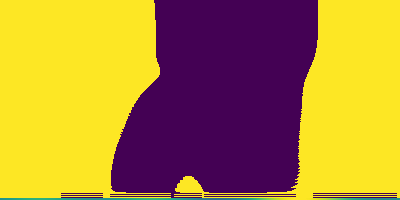
\includegraphics[interpolate=false,width=1.000000in,height=1.000000in]{burgers_rollout_fnn_pred_0.01-img0.png}}%
\end{pgfscope}%
\begin{pgfscope}%
\pgfsetbuttcap%
\pgfsetroundjoin%
\definecolor{currentfill}{rgb}{0.000000,0.000000,0.000000}%
\pgfsetfillcolor{currentfill}%
\pgfsetlinewidth{0.803000pt}%
\definecolor{currentstroke}{rgb}{0.000000,0.000000,0.000000}%
\pgfsetstrokecolor{currentstroke}%
\pgfsetdash{}{0pt}%
\pgfsys@defobject{currentmarker}{\pgfqpoint{0.000000in}{-0.048611in}}{\pgfqpoint{0.000000in}{0.000000in}}{%
\pgfpathmoveto{\pgfqpoint{0.000000in}{0.000000in}}%
\pgfpathlineto{\pgfqpoint{0.000000in}{-0.048611in}}%
\pgfusepath{stroke,fill}%
}%
\begin{pgfscope}%
\pgfsys@transformshift{0.726837in}{0.517039in}%
\pgfsys@useobject{currentmarker}{}%
\end{pgfscope}%
\end{pgfscope}%
\begin{pgfscope}%
\definecolor{textcolor}{rgb}{0.000000,0.000000,0.000000}%
\pgfsetstrokecolor{textcolor}%
\pgfsetfillcolor{textcolor}%
\pgftext[x=0.726837in,y=0.419816in,,top]{\color{textcolor}\rmfamily\fontsize{12.000000}{14.400000}\selectfont 0}%
\end{pgfscope}%
\begin{pgfscope}%
\pgfsetbuttcap%
\pgfsetroundjoin%
\definecolor{currentfill}{rgb}{0.000000,0.000000,0.000000}%
\pgfsetfillcolor{currentfill}%
\pgfsetlinewidth{0.803000pt}%
\definecolor{currentstroke}{rgb}{0.000000,0.000000,0.000000}%
\pgfsetstrokecolor{currentstroke}%
\pgfsetdash{}{0pt}%
\pgfsys@defobject{currentmarker}{\pgfqpoint{0.000000in}{-0.048611in}}{\pgfqpoint{0.000000in}{0.000000in}}{%
\pgfpathmoveto{\pgfqpoint{0.000000in}{0.000000in}}%
\pgfpathlineto{\pgfqpoint{0.000000in}{-0.048611in}}%
\pgfusepath{stroke,fill}%
}%
\begin{pgfscope}%
\pgfsys@transformshift{1.495432in}{0.517039in}%
\pgfsys@useobject{currentmarker}{}%
\end{pgfscope}%
\end{pgfscope}%
\begin{pgfscope}%
\definecolor{textcolor}{rgb}{0.000000,0.000000,0.000000}%
\pgfsetstrokecolor{textcolor}%
\pgfsetfillcolor{textcolor}%
\pgftext[x=1.495432in,y=0.419816in,,top]{\color{textcolor}\rmfamily\fontsize{12.000000}{14.400000}\selectfont 1}%
\end{pgfscope}%
\begin{pgfscope}%
\pgfsetbuttcap%
\pgfsetroundjoin%
\definecolor{currentfill}{rgb}{0.000000,0.000000,0.000000}%
\pgfsetfillcolor{currentfill}%
\pgfsetlinewidth{0.803000pt}%
\definecolor{currentstroke}{rgb}{0.000000,0.000000,0.000000}%
\pgfsetstrokecolor{currentstroke}%
\pgfsetdash{}{0pt}%
\pgfsys@defobject{currentmarker}{\pgfqpoint{0.000000in}{-0.048611in}}{\pgfqpoint{0.000000in}{0.000000in}}{%
\pgfpathmoveto{\pgfqpoint{0.000000in}{0.000000in}}%
\pgfpathlineto{\pgfqpoint{0.000000in}{-0.048611in}}%
\pgfusepath{stroke,fill}%
}%
\begin{pgfscope}%
\pgfsys@transformshift{2.264026in}{0.517039in}%
\pgfsys@useobject{currentmarker}{}%
\end{pgfscope}%
\end{pgfscope}%
\begin{pgfscope}%
\definecolor{textcolor}{rgb}{0.000000,0.000000,0.000000}%
\pgfsetstrokecolor{textcolor}%
\pgfsetfillcolor{textcolor}%
\pgftext[x=2.264026in,y=0.419816in,,top]{\color{textcolor}\rmfamily\fontsize{12.000000}{14.400000}\selectfont 2}%
\end{pgfscope}%
\begin{pgfscope}%
\definecolor{textcolor}{rgb}{0.000000,0.000000,0.000000}%
\pgfsetstrokecolor{textcolor}%
\pgfsetfillcolor{textcolor}%
\pgftext[x=1.495432in,y=0.202965in,,top]{\color{textcolor}\rmfamily\fontsize{12.000000}{14.400000}\selectfont Space}%
\end{pgfscope}%
\begin{pgfscope}%
\pgfsetbuttcap%
\pgfsetroundjoin%
\definecolor{currentfill}{rgb}{0.000000,0.000000,0.000000}%
\pgfsetfillcolor{currentfill}%
\pgfsetlinewidth{0.803000pt}%
\definecolor{currentstroke}{rgb}{0.000000,0.000000,0.000000}%
\pgfsetstrokecolor{currentstroke}%
\pgfsetdash{}{0pt}%
\pgfsys@defobject{currentmarker}{\pgfqpoint{-0.048611in}{0.000000in}}{\pgfqpoint{-0.000000in}{0.000000in}}{%
\pgfpathmoveto{\pgfqpoint{-0.000000in}{0.000000in}}%
\pgfpathlineto{\pgfqpoint{-0.048611in}{0.000000in}}%
\pgfusepath{stroke,fill}%
}%
\begin{pgfscope}%
\pgfsys@transformshift{0.726837in}{0.517039in}%
\pgfsys@useobject{currentmarker}{}%
\end{pgfscope}%
\end{pgfscope}%
\begin{pgfscope}%
\definecolor{textcolor}{rgb}{0.000000,0.000000,0.000000}%
\pgfsetstrokecolor{textcolor}%
\pgfsetfillcolor{textcolor}%
\pgftext[x=0.364559in, y=0.453725in, left, base]{\color{textcolor}\rmfamily\fontsize{12.000000}{14.400000}\selectfont 0.0}%
\end{pgfscope}%
\begin{pgfscope}%
\pgfsetbuttcap%
\pgfsetroundjoin%
\definecolor{currentfill}{rgb}{0.000000,0.000000,0.000000}%
\pgfsetfillcolor{currentfill}%
\pgfsetlinewidth{0.803000pt}%
\definecolor{currentstroke}{rgb}{0.000000,0.000000,0.000000}%
\pgfsetstrokecolor{currentstroke}%
\pgfsetdash{}{0pt}%
\pgfsys@defobject{currentmarker}{\pgfqpoint{-0.048611in}{0.000000in}}{\pgfqpoint{-0.000000in}{0.000000in}}{%
\pgfpathmoveto{\pgfqpoint{-0.000000in}{0.000000in}}%
\pgfpathlineto{\pgfqpoint{-0.048611in}{0.000000in}}%
\pgfusepath{stroke,fill}%
}%
\begin{pgfscope}%
\pgfsys@transformshift{0.726837in}{0.861533in}%
\pgfsys@useobject{currentmarker}{}%
\end{pgfscope}%
\end{pgfscope}%
\begin{pgfscope}%
\definecolor{textcolor}{rgb}{0.000000,0.000000,0.000000}%
\pgfsetstrokecolor{textcolor}%
\pgfsetfillcolor{textcolor}%
\pgftext[x=0.364559in, y=0.798219in, left, base]{\color{textcolor}\rmfamily\fontsize{12.000000}{14.400000}\selectfont 2.5}%
\end{pgfscope}%
\begin{pgfscope}%
\pgfsetbuttcap%
\pgfsetroundjoin%
\definecolor{currentfill}{rgb}{0.000000,0.000000,0.000000}%
\pgfsetfillcolor{currentfill}%
\pgfsetlinewidth{0.803000pt}%
\definecolor{currentstroke}{rgb}{0.000000,0.000000,0.000000}%
\pgfsetstrokecolor{currentstroke}%
\pgfsetdash{}{0pt}%
\pgfsys@defobject{currentmarker}{\pgfqpoint{-0.048611in}{0.000000in}}{\pgfqpoint{-0.000000in}{0.000000in}}{%
\pgfpathmoveto{\pgfqpoint{-0.000000in}{0.000000in}}%
\pgfpathlineto{\pgfqpoint{-0.048611in}{0.000000in}}%
\pgfusepath{stroke,fill}%
}%
\begin{pgfscope}%
\pgfsys@transformshift{0.726837in}{1.206027in}%
\pgfsys@useobject{currentmarker}{}%
\end{pgfscope}%
\end{pgfscope}%
\begin{pgfscope}%
\definecolor{textcolor}{rgb}{0.000000,0.000000,0.000000}%
\pgfsetstrokecolor{textcolor}%
\pgfsetfillcolor{textcolor}%
\pgftext[x=0.364559in, y=1.142714in, left, base]{\color{textcolor}\rmfamily\fontsize{12.000000}{14.400000}\selectfont 5.0}%
\end{pgfscope}%
\begin{pgfscope}%
\pgfsetbuttcap%
\pgfsetroundjoin%
\definecolor{currentfill}{rgb}{0.000000,0.000000,0.000000}%
\pgfsetfillcolor{currentfill}%
\pgfsetlinewidth{0.803000pt}%
\definecolor{currentstroke}{rgb}{0.000000,0.000000,0.000000}%
\pgfsetstrokecolor{currentstroke}%
\pgfsetdash{}{0pt}%
\pgfsys@defobject{currentmarker}{\pgfqpoint{-0.048611in}{0.000000in}}{\pgfqpoint{-0.000000in}{0.000000in}}{%
\pgfpathmoveto{\pgfqpoint{-0.000000in}{0.000000in}}%
\pgfpathlineto{\pgfqpoint{-0.048611in}{0.000000in}}%
\pgfusepath{stroke,fill}%
}%
\begin{pgfscope}%
\pgfsys@transformshift{0.726837in}{1.550522in}%
\pgfsys@useobject{currentmarker}{}%
\end{pgfscope}%
\end{pgfscope}%
\begin{pgfscope}%
\definecolor{textcolor}{rgb}{0.000000,0.000000,0.000000}%
\pgfsetstrokecolor{textcolor}%
\pgfsetfillcolor{textcolor}%
\pgftext[x=0.364559in, y=1.487208in, left, base]{\color{textcolor}\rmfamily\fontsize{12.000000}{14.400000}\selectfont 7.5}%
\end{pgfscope}%
\begin{pgfscope}%
\pgfsetbuttcap%
\pgfsetroundjoin%
\definecolor{currentfill}{rgb}{0.000000,0.000000,0.000000}%
\pgfsetfillcolor{currentfill}%
\pgfsetlinewidth{0.803000pt}%
\definecolor{currentstroke}{rgb}{0.000000,0.000000,0.000000}%
\pgfsetstrokecolor{currentstroke}%
\pgfsetdash{}{0pt}%
\pgfsys@defobject{currentmarker}{\pgfqpoint{-0.048611in}{0.000000in}}{\pgfqpoint{-0.000000in}{0.000000in}}{%
\pgfpathmoveto{\pgfqpoint{-0.000000in}{0.000000in}}%
\pgfpathlineto{\pgfqpoint{-0.048611in}{0.000000in}}%
\pgfusepath{stroke,fill}%
}%
\begin{pgfscope}%
\pgfsys@transformshift{0.726837in}{1.895016in}%
\pgfsys@useobject{currentmarker}{}%
\end{pgfscope}%
\end{pgfscope}%
\begin{pgfscope}%
\definecolor{textcolor}{rgb}{0.000000,0.000000,0.000000}%
\pgfsetstrokecolor{textcolor}%
\pgfsetfillcolor{textcolor}%
\pgftext[x=0.258521in, y=1.831702in, left, base]{\color{textcolor}\rmfamily\fontsize{12.000000}{14.400000}\selectfont 10.0}%
\end{pgfscope}%
\begin{pgfscope}%
\definecolor{textcolor}{rgb}{0.000000,0.000000,0.000000}%
\pgfsetstrokecolor{textcolor}%
\pgfsetfillcolor{textcolor}%
\pgftext[x=0.202965in,y=1.206027in,,bottom,rotate=90.000000]{\color{textcolor}\rmfamily\fontsize{12.000000}{14.400000}\selectfont Time}%
\end{pgfscope}%
\begin{pgfscope}%
\pgfsetrectcap%
\pgfsetmiterjoin%
\pgfsetlinewidth{0.803000pt}%
\definecolor{currentstroke}{rgb}{0.000000,0.000000,0.000000}%
\pgfsetstrokecolor{currentstroke}%
\pgfsetdash{}{0pt}%
\pgfpathmoveto{\pgfqpoint{0.726837in}{0.517039in}}%
\pgfpathlineto{\pgfqpoint{0.726837in}{1.895016in}}%
\pgfusepath{stroke}%
\end{pgfscope}%
\begin{pgfscope}%
\pgfsetrectcap%
\pgfsetmiterjoin%
\pgfsetlinewidth{0.803000pt}%
\definecolor{currentstroke}{rgb}{0.000000,0.000000,0.000000}%
\pgfsetstrokecolor{currentstroke}%
\pgfsetdash{}{0pt}%
\pgfpathmoveto{\pgfqpoint{2.264026in}{0.517039in}}%
\pgfpathlineto{\pgfqpoint{2.264026in}{1.895016in}}%
\pgfusepath{stroke}%
\end{pgfscope}%
\begin{pgfscope}%
\pgfsetrectcap%
\pgfsetmiterjoin%
\pgfsetlinewidth{0.803000pt}%
\definecolor{currentstroke}{rgb}{0.000000,0.000000,0.000000}%
\pgfsetstrokecolor{currentstroke}%
\pgfsetdash{}{0pt}%
\pgfpathmoveto{\pgfqpoint{0.726837in}{0.517039in}}%
\pgfpathlineto{\pgfqpoint{2.264026in}{0.517039in}}%
\pgfusepath{stroke}%
\end{pgfscope}%
\begin{pgfscope}%
\pgfsetrectcap%
\pgfsetmiterjoin%
\pgfsetlinewidth{0.803000pt}%
\definecolor{currentstroke}{rgb}{0.000000,0.000000,0.000000}%
\pgfsetstrokecolor{currentstroke}%
\pgfsetdash{}{0pt}%
\pgfpathmoveto{\pgfqpoint{0.726837in}{1.895016in}}%
\pgfpathlineto{\pgfqpoint{2.264026in}{1.895016in}}%
\pgfusepath{stroke}%
\end{pgfscope}%
\begin{pgfscope}%
\pgfsetbuttcap%
\pgfsetmiterjoin%
\pgfsetlinewidth{0.000000pt}%
\definecolor{currentstroke}{rgb}{0.000000,0.000000,0.000000}%
\pgfsetstrokecolor{currentstroke}%
\pgfsetstrokeopacity{0.000000}%
\pgfsetdash{}{0pt}%
\pgfpathmoveto{\pgfqpoint{2.393905in}{0.517039in}}%
\pgfpathlineto{\pgfqpoint{2.462804in}{0.517039in}}%
\pgfpathlineto{\pgfqpoint{2.462804in}{1.895016in}}%
\pgfpathlineto{\pgfqpoint{2.393905in}{1.895016in}}%
\pgfpathlineto{\pgfqpoint{2.393905in}{0.517039in}}%
\pgfpathclose%
\pgfusepath{}%
\end{pgfscope}%
\begin{pgfscope}%
\pgfsys@transformshift{2.390000in}{0.520000in}%
\pgftext[left,bottom]{
\includegraphics[interpolate=true,width=0.070000in,height=1.380000in]{burgers_rollout_fnn_pred_0.01-img1.png}}%
\end{pgfscope}%
\begin{pgfscope}%
\pgfsetbuttcap%
\pgfsetroundjoin%
\definecolor{currentfill}{rgb}{0.000000,0.000000,0.000000}%
\pgfsetfillcolor{currentfill}%
\pgfsetlinewidth{0.803000pt}%
\definecolor{currentstroke}{rgb}{0.000000,0.000000,0.000000}%
\pgfsetstrokecolor{currentstroke}%
\pgfsetdash{}{0pt}%
\pgfsys@defobject{currentmarker}{\pgfqpoint{0.000000in}{0.000000in}}{\pgfqpoint{0.048611in}{0.000000in}}{%
\pgfpathmoveto{\pgfqpoint{0.000000in}{0.000000in}}%
\pgfpathlineto{\pgfqpoint{0.048611in}{0.000000in}}%
\pgfusepath{stroke,fill}%
}%
\begin{pgfscope}%
\pgfsys@transformshift{2.462804in}{0.839076in}%
\pgfsys@useobject{currentmarker}{}%
\end{pgfscope}%
\end{pgfscope}%
\begin{pgfscope}%
\definecolor{textcolor}{rgb}{0.000000,0.000000,0.000000}%
\pgfsetstrokecolor{textcolor}%
\pgfsetfillcolor{textcolor}%
\pgftext[x=2.560026in, y=0.775762in, left, base]{\color{textcolor}\rmfamily\fontsize{12.000000}{14.400000}\selectfont \ensuremath{-}0.5}%
\end{pgfscope}%
\begin{pgfscope}%
\pgfsetbuttcap%
\pgfsetroundjoin%
\definecolor{currentfill}{rgb}{0.000000,0.000000,0.000000}%
\pgfsetfillcolor{currentfill}%
\pgfsetlinewidth{0.803000pt}%
\definecolor{currentstroke}{rgb}{0.000000,0.000000,0.000000}%
\pgfsetstrokecolor{currentstroke}%
\pgfsetdash{}{0pt}%
\pgfsys@defobject{currentmarker}{\pgfqpoint{0.000000in}{0.000000in}}{\pgfqpoint{0.048611in}{0.000000in}}{%
\pgfpathmoveto{\pgfqpoint{0.000000in}{0.000000in}}%
\pgfpathlineto{\pgfqpoint{0.048611in}{0.000000in}}%
\pgfusepath{stroke,fill}%
}%
\begin{pgfscope}%
\pgfsys@transformshift{2.462804in}{1.206027in}%
\pgfsys@useobject{currentmarker}{}%
\end{pgfscope}%
\end{pgfscope}%
\begin{pgfscope}%
\definecolor{textcolor}{rgb}{0.000000,0.000000,0.000000}%
\pgfsetstrokecolor{textcolor}%
\pgfsetfillcolor{textcolor}%
\pgftext[x=2.560026in, y=1.142714in, left, base]{\color{textcolor}\rmfamily\fontsize{12.000000}{14.400000}\selectfont 0.0}%
\end{pgfscope}%
\begin{pgfscope}%
\pgfsetbuttcap%
\pgfsetroundjoin%
\definecolor{currentfill}{rgb}{0.000000,0.000000,0.000000}%
\pgfsetfillcolor{currentfill}%
\pgfsetlinewidth{0.803000pt}%
\definecolor{currentstroke}{rgb}{0.000000,0.000000,0.000000}%
\pgfsetstrokecolor{currentstroke}%
\pgfsetdash{}{0pt}%
\pgfsys@defobject{currentmarker}{\pgfqpoint{0.000000in}{0.000000in}}{\pgfqpoint{0.048611in}{0.000000in}}{%
\pgfpathmoveto{\pgfqpoint{0.000000in}{0.000000in}}%
\pgfpathlineto{\pgfqpoint{0.048611in}{0.000000in}}%
\pgfusepath{stroke,fill}%
}%
\begin{pgfscope}%
\pgfsys@transformshift{2.462804in}{1.572979in}%
\pgfsys@useobject{currentmarker}{}%
\end{pgfscope}%
\end{pgfscope}%
\begin{pgfscope}%
\definecolor{textcolor}{rgb}{0.000000,0.000000,0.000000}%
\pgfsetstrokecolor{textcolor}%
\pgfsetfillcolor{textcolor}%
\pgftext[x=2.560026in, y=1.509665in, left, base]{\color{textcolor}\rmfamily\fontsize{12.000000}{14.400000}\selectfont 0.5}%
\end{pgfscope}%
\begin{pgfscope}%
\pgfsetrectcap%
\pgfsetmiterjoin%
\pgfsetlinewidth{0.803000pt}%
\definecolor{currentstroke}{rgb}{0.000000,0.000000,0.000000}%
\pgfsetstrokecolor{currentstroke}%
\pgfsetdash{}{0pt}%
\pgfpathmoveto{\pgfqpoint{2.393905in}{0.517039in}}%
\pgfpathlineto{\pgfqpoint{2.428354in}{0.517039in}}%
\pgfpathlineto{\pgfqpoint{2.462804in}{0.517039in}}%
\pgfpathlineto{\pgfqpoint{2.462804in}{1.895016in}}%
\pgfpathlineto{\pgfqpoint{2.428354in}{1.895016in}}%
\pgfpathlineto{\pgfqpoint{2.393905in}{1.895016in}}%
\pgfpathlineto{\pgfqpoint{2.393905in}{0.517039in}}%
\pgfpathclose%
\pgfusepath{stroke}%
\end{pgfscope}%
\end{pgfpicture}%
\makeatother%
\endgroup%

      \end{adjustbox}
      \caption{SpectralSVR prediction.}\label{fig:comp_fnn_pred_0.01}
    \end{subfigure}
    \begin{subfigure}{0.49\linewidth}
      \begin{adjustbox}{width=\linewidth}
        \begingroup%
\makeatletter%
\begin{pgfpicture}%
\pgfpathrectangle{\pgfpointorigin}{\pgfqpoint{3.000000in}{2.000000in}}%
\pgfusepath{use as bounding box, clip}%
\begin{pgfscope}%
\pgfsetbuttcap%
\pgfsetmiterjoin%
\pgfsetlinewidth{0.000000pt}%
\definecolor{currentstroke}{rgb}{0.000000,0.000000,0.000000}%
\pgfsetstrokecolor{currentstroke}%
\pgfsetstrokeopacity{0.000000}%
\pgfsetdash{}{0pt}%
\pgfpathmoveto{\pgfqpoint{0.000000in}{0.000000in}}%
\pgfpathlineto{\pgfqpoint{3.000000in}{0.000000in}}%
\pgfpathlineto{\pgfqpoint{3.000000in}{2.000000in}}%
\pgfpathlineto{\pgfqpoint{0.000000in}{2.000000in}}%
\pgfpathlineto{\pgfqpoint{0.000000in}{0.000000in}}%
\pgfpathclose%
\pgfusepath{}%
\end{pgfscope}%
\begin{pgfscope}%
\pgfsetbuttcap%
\pgfsetmiterjoin%
\pgfsetlinewidth{0.000000pt}%
\definecolor{currentstroke}{rgb}{0.000000,0.000000,0.000000}%
\pgfsetstrokecolor{currentstroke}%
\pgfsetstrokeopacity{0.000000}%
\pgfsetdash{}{0pt}%
\pgfpathmoveto{\pgfqpoint{0.726837in}{0.517039in}}%
\pgfpathlineto{\pgfqpoint{2.264026in}{0.517039in}}%
\pgfpathlineto{\pgfqpoint{2.264026in}{1.895016in}}%
\pgfpathlineto{\pgfqpoint{0.726837in}{1.895016in}}%
\pgfpathlineto{\pgfqpoint{0.726837in}{0.517039in}}%
\pgfpathclose%
\pgfusepath{}%
\end{pgfscope}%
\begin{pgfscope}%
\pgfpathrectangle{\pgfqpoint{0.726837in}{0.517039in}}{\pgfqpoint{1.537189in}{1.377978in}}%
\pgfusepath{clip}%
\pgfsys@transformcm{1.537189}{0.000000}{0.000000}{1.377978}{0.726837in}{0.517039in}%
\pgftext[left,bottom]{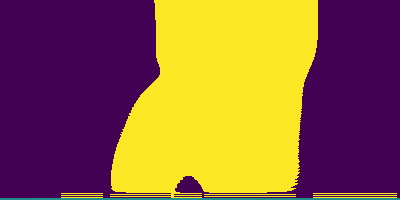
\includegraphics[interpolate=false,width=1.000000in,height=1.000000in]{burgers_rollout_fnn_diff_0.01-img0.png}}%
\end{pgfscope}%
\begin{pgfscope}%
\pgfsetbuttcap%
\pgfsetroundjoin%
\definecolor{currentfill}{rgb}{0.000000,0.000000,0.000000}%
\pgfsetfillcolor{currentfill}%
\pgfsetlinewidth{0.803000pt}%
\definecolor{currentstroke}{rgb}{0.000000,0.000000,0.000000}%
\pgfsetstrokecolor{currentstroke}%
\pgfsetdash{}{0pt}%
\pgfsys@defobject{currentmarker}{\pgfqpoint{0.000000in}{-0.048611in}}{\pgfqpoint{0.000000in}{0.000000in}}{%
\pgfpathmoveto{\pgfqpoint{0.000000in}{0.000000in}}%
\pgfpathlineto{\pgfqpoint{0.000000in}{-0.048611in}}%
\pgfusepath{stroke,fill}%
}%
\begin{pgfscope}%
\pgfsys@transformshift{0.726837in}{0.517039in}%
\pgfsys@useobject{currentmarker}{}%
\end{pgfscope}%
\end{pgfscope}%
\begin{pgfscope}%
\definecolor{textcolor}{rgb}{0.000000,0.000000,0.000000}%
\pgfsetstrokecolor{textcolor}%
\pgfsetfillcolor{textcolor}%
\pgftext[x=0.726837in,y=0.419816in,,top]{\color{textcolor}\rmfamily\fontsize{12.000000}{14.400000}\selectfont 0}%
\end{pgfscope}%
\begin{pgfscope}%
\pgfsetbuttcap%
\pgfsetroundjoin%
\definecolor{currentfill}{rgb}{0.000000,0.000000,0.000000}%
\pgfsetfillcolor{currentfill}%
\pgfsetlinewidth{0.803000pt}%
\definecolor{currentstroke}{rgb}{0.000000,0.000000,0.000000}%
\pgfsetstrokecolor{currentstroke}%
\pgfsetdash{}{0pt}%
\pgfsys@defobject{currentmarker}{\pgfqpoint{0.000000in}{-0.048611in}}{\pgfqpoint{0.000000in}{0.000000in}}{%
\pgfpathmoveto{\pgfqpoint{0.000000in}{0.000000in}}%
\pgfpathlineto{\pgfqpoint{0.000000in}{-0.048611in}}%
\pgfusepath{stroke,fill}%
}%
\begin{pgfscope}%
\pgfsys@transformshift{1.495432in}{0.517039in}%
\pgfsys@useobject{currentmarker}{}%
\end{pgfscope}%
\end{pgfscope}%
\begin{pgfscope}%
\definecolor{textcolor}{rgb}{0.000000,0.000000,0.000000}%
\pgfsetstrokecolor{textcolor}%
\pgfsetfillcolor{textcolor}%
\pgftext[x=1.495432in,y=0.419816in,,top]{\color{textcolor}\rmfamily\fontsize{12.000000}{14.400000}\selectfont 1}%
\end{pgfscope}%
\begin{pgfscope}%
\pgfsetbuttcap%
\pgfsetroundjoin%
\definecolor{currentfill}{rgb}{0.000000,0.000000,0.000000}%
\pgfsetfillcolor{currentfill}%
\pgfsetlinewidth{0.803000pt}%
\definecolor{currentstroke}{rgb}{0.000000,0.000000,0.000000}%
\pgfsetstrokecolor{currentstroke}%
\pgfsetdash{}{0pt}%
\pgfsys@defobject{currentmarker}{\pgfqpoint{0.000000in}{-0.048611in}}{\pgfqpoint{0.000000in}{0.000000in}}{%
\pgfpathmoveto{\pgfqpoint{0.000000in}{0.000000in}}%
\pgfpathlineto{\pgfqpoint{0.000000in}{-0.048611in}}%
\pgfusepath{stroke,fill}%
}%
\begin{pgfscope}%
\pgfsys@transformshift{2.264026in}{0.517039in}%
\pgfsys@useobject{currentmarker}{}%
\end{pgfscope}%
\end{pgfscope}%
\begin{pgfscope}%
\definecolor{textcolor}{rgb}{0.000000,0.000000,0.000000}%
\pgfsetstrokecolor{textcolor}%
\pgfsetfillcolor{textcolor}%
\pgftext[x=2.264026in,y=0.419816in,,top]{\color{textcolor}\rmfamily\fontsize{12.000000}{14.400000}\selectfont 2}%
\end{pgfscope}%
\begin{pgfscope}%
\definecolor{textcolor}{rgb}{0.000000,0.000000,0.000000}%
\pgfsetstrokecolor{textcolor}%
\pgfsetfillcolor{textcolor}%
\pgftext[x=1.495432in,y=0.202965in,,top]{\color{textcolor}\rmfamily\fontsize{12.000000}{14.400000}\selectfont Space}%
\end{pgfscope}%
\begin{pgfscope}%
\pgfsetbuttcap%
\pgfsetroundjoin%
\definecolor{currentfill}{rgb}{0.000000,0.000000,0.000000}%
\pgfsetfillcolor{currentfill}%
\pgfsetlinewidth{0.803000pt}%
\definecolor{currentstroke}{rgb}{0.000000,0.000000,0.000000}%
\pgfsetstrokecolor{currentstroke}%
\pgfsetdash{}{0pt}%
\pgfsys@defobject{currentmarker}{\pgfqpoint{-0.048611in}{0.000000in}}{\pgfqpoint{-0.000000in}{0.000000in}}{%
\pgfpathmoveto{\pgfqpoint{-0.000000in}{0.000000in}}%
\pgfpathlineto{\pgfqpoint{-0.048611in}{0.000000in}}%
\pgfusepath{stroke,fill}%
}%
\begin{pgfscope}%
\pgfsys@transformshift{0.726837in}{0.517039in}%
\pgfsys@useobject{currentmarker}{}%
\end{pgfscope}%
\end{pgfscope}%
\begin{pgfscope}%
\definecolor{textcolor}{rgb}{0.000000,0.000000,0.000000}%
\pgfsetstrokecolor{textcolor}%
\pgfsetfillcolor{textcolor}%
\pgftext[x=0.364559in, y=0.453725in, left, base]{\color{textcolor}\rmfamily\fontsize{12.000000}{14.400000}\selectfont 0.0}%
\end{pgfscope}%
\begin{pgfscope}%
\pgfsetbuttcap%
\pgfsetroundjoin%
\definecolor{currentfill}{rgb}{0.000000,0.000000,0.000000}%
\pgfsetfillcolor{currentfill}%
\pgfsetlinewidth{0.803000pt}%
\definecolor{currentstroke}{rgb}{0.000000,0.000000,0.000000}%
\pgfsetstrokecolor{currentstroke}%
\pgfsetdash{}{0pt}%
\pgfsys@defobject{currentmarker}{\pgfqpoint{-0.048611in}{0.000000in}}{\pgfqpoint{-0.000000in}{0.000000in}}{%
\pgfpathmoveto{\pgfqpoint{-0.000000in}{0.000000in}}%
\pgfpathlineto{\pgfqpoint{-0.048611in}{0.000000in}}%
\pgfusepath{stroke,fill}%
}%
\begin{pgfscope}%
\pgfsys@transformshift{0.726837in}{0.861533in}%
\pgfsys@useobject{currentmarker}{}%
\end{pgfscope}%
\end{pgfscope}%
\begin{pgfscope}%
\definecolor{textcolor}{rgb}{0.000000,0.000000,0.000000}%
\pgfsetstrokecolor{textcolor}%
\pgfsetfillcolor{textcolor}%
\pgftext[x=0.364559in, y=0.798219in, left, base]{\color{textcolor}\rmfamily\fontsize{12.000000}{14.400000}\selectfont 2.5}%
\end{pgfscope}%
\begin{pgfscope}%
\pgfsetbuttcap%
\pgfsetroundjoin%
\definecolor{currentfill}{rgb}{0.000000,0.000000,0.000000}%
\pgfsetfillcolor{currentfill}%
\pgfsetlinewidth{0.803000pt}%
\definecolor{currentstroke}{rgb}{0.000000,0.000000,0.000000}%
\pgfsetstrokecolor{currentstroke}%
\pgfsetdash{}{0pt}%
\pgfsys@defobject{currentmarker}{\pgfqpoint{-0.048611in}{0.000000in}}{\pgfqpoint{-0.000000in}{0.000000in}}{%
\pgfpathmoveto{\pgfqpoint{-0.000000in}{0.000000in}}%
\pgfpathlineto{\pgfqpoint{-0.048611in}{0.000000in}}%
\pgfusepath{stroke,fill}%
}%
\begin{pgfscope}%
\pgfsys@transformshift{0.726837in}{1.206027in}%
\pgfsys@useobject{currentmarker}{}%
\end{pgfscope}%
\end{pgfscope}%
\begin{pgfscope}%
\definecolor{textcolor}{rgb}{0.000000,0.000000,0.000000}%
\pgfsetstrokecolor{textcolor}%
\pgfsetfillcolor{textcolor}%
\pgftext[x=0.364559in, y=1.142714in, left, base]{\color{textcolor}\rmfamily\fontsize{12.000000}{14.400000}\selectfont 5.0}%
\end{pgfscope}%
\begin{pgfscope}%
\pgfsetbuttcap%
\pgfsetroundjoin%
\definecolor{currentfill}{rgb}{0.000000,0.000000,0.000000}%
\pgfsetfillcolor{currentfill}%
\pgfsetlinewidth{0.803000pt}%
\definecolor{currentstroke}{rgb}{0.000000,0.000000,0.000000}%
\pgfsetstrokecolor{currentstroke}%
\pgfsetdash{}{0pt}%
\pgfsys@defobject{currentmarker}{\pgfqpoint{-0.048611in}{0.000000in}}{\pgfqpoint{-0.000000in}{0.000000in}}{%
\pgfpathmoveto{\pgfqpoint{-0.000000in}{0.000000in}}%
\pgfpathlineto{\pgfqpoint{-0.048611in}{0.000000in}}%
\pgfusepath{stroke,fill}%
}%
\begin{pgfscope}%
\pgfsys@transformshift{0.726837in}{1.550522in}%
\pgfsys@useobject{currentmarker}{}%
\end{pgfscope}%
\end{pgfscope}%
\begin{pgfscope}%
\definecolor{textcolor}{rgb}{0.000000,0.000000,0.000000}%
\pgfsetstrokecolor{textcolor}%
\pgfsetfillcolor{textcolor}%
\pgftext[x=0.364559in, y=1.487208in, left, base]{\color{textcolor}\rmfamily\fontsize{12.000000}{14.400000}\selectfont 7.5}%
\end{pgfscope}%
\begin{pgfscope}%
\pgfsetbuttcap%
\pgfsetroundjoin%
\definecolor{currentfill}{rgb}{0.000000,0.000000,0.000000}%
\pgfsetfillcolor{currentfill}%
\pgfsetlinewidth{0.803000pt}%
\definecolor{currentstroke}{rgb}{0.000000,0.000000,0.000000}%
\pgfsetstrokecolor{currentstroke}%
\pgfsetdash{}{0pt}%
\pgfsys@defobject{currentmarker}{\pgfqpoint{-0.048611in}{0.000000in}}{\pgfqpoint{-0.000000in}{0.000000in}}{%
\pgfpathmoveto{\pgfqpoint{-0.000000in}{0.000000in}}%
\pgfpathlineto{\pgfqpoint{-0.048611in}{0.000000in}}%
\pgfusepath{stroke,fill}%
}%
\begin{pgfscope}%
\pgfsys@transformshift{0.726837in}{1.895016in}%
\pgfsys@useobject{currentmarker}{}%
\end{pgfscope}%
\end{pgfscope}%
\begin{pgfscope}%
\definecolor{textcolor}{rgb}{0.000000,0.000000,0.000000}%
\pgfsetstrokecolor{textcolor}%
\pgfsetfillcolor{textcolor}%
\pgftext[x=0.258521in, y=1.831702in, left, base]{\color{textcolor}\rmfamily\fontsize{12.000000}{14.400000}\selectfont 10.0}%
\end{pgfscope}%
\begin{pgfscope}%
\definecolor{textcolor}{rgb}{0.000000,0.000000,0.000000}%
\pgfsetstrokecolor{textcolor}%
\pgfsetfillcolor{textcolor}%
\pgftext[x=0.202965in,y=1.206027in,,bottom,rotate=90.000000]{\color{textcolor}\rmfamily\fontsize{12.000000}{14.400000}\selectfont Time}%
\end{pgfscope}%
\begin{pgfscope}%
\pgfsetrectcap%
\pgfsetmiterjoin%
\pgfsetlinewidth{0.803000pt}%
\definecolor{currentstroke}{rgb}{0.000000,0.000000,0.000000}%
\pgfsetstrokecolor{currentstroke}%
\pgfsetdash{}{0pt}%
\pgfpathmoveto{\pgfqpoint{0.726837in}{0.517039in}}%
\pgfpathlineto{\pgfqpoint{0.726837in}{1.895016in}}%
\pgfusepath{stroke}%
\end{pgfscope}%
\begin{pgfscope}%
\pgfsetrectcap%
\pgfsetmiterjoin%
\pgfsetlinewidth{0.803000pt}%
\definecolor{currentstroke}{rgb}{0.000000,0.000000,0.000000}%
\pgfsetstrokecolor{currentstroke}%
\pgfsetdash{}{0pt}%
\pgfpathmoveto{\pgfqpoint{2.264026in}{0.517039in}}%
\pgfpathlineto{\pgfqpoint{2.264026in}{1.895016in}}%
\pgfusepath{stroke}%
\end{pgfscope}%
\begin{pgfscope}%
\pgfsetrectcap%
\pgfsetmiterjoin%
\pgfsetlinewidth{0.803000pt}%
\definecolor{currentstroke}{rgb}{0.000000,0.000000,0.000000}%
\pgfsetstrokecolor{currentstroke}%
\pgfsetdash{}{0pt}%
\pgfpathmoveto{\pgfqpoint{0.726837in}{0.517039in}}%
\pgfpathlineto{\pgfqpoint{2.264026in}{0.517039in}}%
\pgfusepath{stroke}%
\end{pgfscope}%
\begin{pgfscope}%
\pgfsetrectcap%
\pgfsetmiterjoin%
\pgfsetlinewidth{0.803000pt}%
\definecolor{currentstroke}{rgb}{0.000000,0.000000,0.000000}%
\pgfsetstrokecolor{currentstroke}%
\pgfsetdash{}{0pt}%
\pgfpathmoveto{\pgfqpoint{0.726837in}{1.895016in}}%
\pgfpathlineto{\pgfqpoint{2.264026in}{1.895016in}}%
\pgfusepath{stroke}%
\end{pgfscope}%
\begin{pgfscope}%
\pgfsetbuttcap%
\pgfsetmiterjoin%
\pgfsetlinewidth{0.000000pt}%
\definecolor{currentstroke}{rgb}{0.000000,0.000000,0.000000}%
\pgfsetstrokecolor{currentstroke}%
\pgfsetstrokeopacity{0.000000}%
\pgfsetdash{}{0pt}%
\pgfpathmoveto{\pgfqpoint{2.393905in}{0.517039in}}%
\pgfpathlineto{\pgfqpoint{2.462804in}{0.517039in}}%
\pgfpathlineto{\pgfqpoint{2.462804in}{1.895016in}}%
\pgfpathlineto{\pgfqpoint{2.393905in}{1.895016in}}%
\pgfpathlineto{\pgfqpoint{2.393905in}{0.517039in}}%
\pgfpathclose%
\pgfusepath{}%
\end{pgfscope}%
\begin{pgfscope}%
\pgfsys@transformshift{2.390000in}{0.520000in}%
\pgftext[left,bottom]{
\includegraphics[interpolate=true,width=0.070000in,height=1.380000in]{burgers_rollout_fnn_diff_0.01-img1.png}}%
\end{pgfscope}%
\begin{pgfscope}%
\pgfsetbuttcap%
\pgfsetroundjoin%
\definecolor{currentfill}{rgb}{0.000000,0.000000,0.000000}%
\pgfsetfillcolor{currentfill}%
\pgfsetlinewidth{0.803000pt}%
\definecolor{currentstroke}{rgb}{0.000000,0.000000,0.000000}%
\pgfsetstrokecolor{currentstroke}%
\pgfsetdash{}{0pt}%
\pgfsys@defobject{currentmarker}{\pgfqpoint{0.000000in}{0.000000in}}{\pgfqpoint{0.048611in}{0.000000in}}{%
\pgfpathmoveto{\pgfqpoint{0.000000in}{0.000000in}}%
\pgfpathlineto{\pgfqpoint{0.048611in}{0.000000in}}%
\pgfusepath{stroke,fill}%
}%
\begin{pgfscope}%
\pgfsys@transformshift{2.462804in}{0.839076in}%
\pgfsys@useobject{currentmarker}{}%
\end{pgfscope}%
\end{pgfscope}%
\begin{pgfscope}%
\definecolor{textcolor}{rgb}{0.000000,0.000000,0.000000}%
\pgfsetstrokecolor{textcolor}%
\pgfsetfillcolor{textcolor}%
\pgftext[x=2.560026in, y=0.775762in, left, base]{\color{textcolor}\rmfamily\fontsize{12.000000}{14.400000}\selectfont \ensuremath{-}0.5}%
\end{pgfscope}%
\begin{pgfscope}%
\pgfsetbuttcap%
\pgfsetroundjoin%
\definecolor{currentfill}{rgb}{0.000000,0.000000,0.000000}%
\pgfsetfillcolor{currentfill}%
\pgfsetlinewidth{0.803000pt}%
\definecolor{currentstroke}{rgb}{0.000000,0.000000,0.000000}%
\pgfsetstrokecolor{currentstroke}%
\pgfsetdash{}{0pt}%
\pgfsys@defobject{currentmarker}{\pgfqpoint{0.000000in}{0.000000in}}{\pgfqpoint{0.048611in}{0.000000in}}{%
\pgfpathmoveto{\pgfqpoint{0.000000in}{0.000000in}}%
\pgfpathlineto{\pgfqpoint{0.048611in}{0.000000in}}%
\pgfusepath{stroke,fill}%
}%
\begin{pgfscope}%
\pgfsys@transformshift{2.462804in}{1.206027in}%
\pgfsys@useobject{currentmarker}{}%
\end{pgfscope}%
\end{pgfscope}%
\begin{pgfscope}%
\definecolor{textcolor}{rgb}{0.000000,0.000000,0.000000}%
\pgfsetstrokecolor{textcolor}%
\pgfsetfillcolor{textcolor}%
\pgftext[x=2.560026in, y=1.142714in, left, base]{\color{textcolor}\rmfamily\fontsize{12.000000}{14.400000}\selectfont 0.0}%
\end{pgfscope}%
\begin{pgfscope}%
\pgfsetbuttcap%
\pgfsetroundjoin%
\definecolor{currentfill}{rgb}{0.000000,0.000000,0.000000}%
\pgfsetfillcolor{currentfill}%
\pgfsetlinewidth{0.803000pt}%
\definecolor{currentstroke}{rgb}{0.000000,0.000000,0.000000}%
\pgfsetstrokecolor{currentstroke}%
\pgfsetdash{}{0pt}%
\pgfsys@defobject{currentmarker}{\pgfqpoint{0.000000in}{0.000000in}}{\pgfqpoint{0.048611in}{0.000000in}}{%
\pgfpathmoveto{\pgfqpoint{0.000000in}{0.000000in}}%
\pgfpathlineto{\pgfqpoint{0.048611in}{0.000000in}}%
\pgfusepath{stroke,fill}%
}%
\begin{pgfscope}%
\pgfsys@transformshift{2.462804in}{1.572979in}%
\pgfsys@useobject{currentmarker}{}%
\end{pgfscope}%
\end{pgfscope}%
\begin{pgfscope}%
\definecolor{textcolor}{rgb}{0.000000,0.000000,0.000000}%
\pgfsetstrokecolor{textcolor}%
\pgfsetfillcolor{textcolor}%
\pgftext[x=2.560026in, y=1.509665in, left, base]{\color{textcolor}\rmfamily\fontsize{12.000000}{14.400000}\selectfont 0.5}%
\end{pgfscope}%
\begin{pgfscope}%
\pgfsetrectcap%
\pgfsetmiterjoin%
\pgfsetlinewidth{0.803000pt}%
\definecolor{currentstroke}{rgb}{0.000000,0.000000,0.000000}%
\pgfsetstrokecolor{currentstroke}%
\pgfsetdash{}{0pt}%
\pgfpathmoveto{\pgfqpoint{2.393905in}{0.517039in}}%
\pgfpathlineto{\pgfqpoint{2.428354in}{0.517039in}}%
\pgfpathlineto{\pgfqpoint{2.462804in}{0.517039in}}%
\pgfpathlineto{\pgfqpoint{2.462804in}{1.895016in}}%
\pgfpathlineto{\pgfqpoint{2.428354in}{1.895016in}}%
\pgfpathlineto{\pgfqpoint{2.393905in}{1.895016in}}%
\pgfpathlineto{\pgfqpoint{2.393905in}{0.517039in}}%
\pgfpathclose%
\pgfusepath{stroke}%
\end{pgfscope}%
\end{pgfpicture}%
\makeatother%
\endgroup%

      \end{adjustbox}
      \caption{SpectralSVR difference with target.}\label{fig:comp_fnn_diff_0.01}
    \end{subfigure}
    \begin{subfigure}{0.49\linewidth}
      \begin{adjustbox}{width=\linewidth}
        \begingroup%
\makeatletter%
\begin{pgfpicture}%
\pgfpathrectangle{\pgfpointorigin}{\pgfqpoint{3.000000in}{2.000000in}}%
\pgfusepath{use as bounding box, clip}%
\begin{pgfscope}%
\pgfsetbuttcap%
\pgfsetmiterjoin%
\pgfsetlinewidth{0.000000pt}%
\definecolor{currentstroke}{rgb}{0.000000,0.000000,0.000000}%
\pgfsetstrokecolor{currentstroke}%
\pgfsetstrokeopacity{0.000000}%
\pgfsetdash{}{0pt}%
\pgfpathmoveto{\pgfqpoint{0.000000in}{0.000000in}}%
\pgfpathlineto{\pgfqpoint{3.000000in}{0.000000in}}%
\pgfpathlineto{\pgfqpoint{3.000000in}{2.000000in}}%
\pgfpathlineto{\pgfqpoint{0.000000in}{2.000000in}}%
\pgfpathlineto{\pgfqpoint{0.000000in}{0.000000in}}%
\pgfpathclose%
\pgfusepath{}%
\end{pgfscope}%
\begin{pgfscope}%
\pgfsetbuttcap%
\pgfsetmiterjoin%
\pgfsetlinewidth{0.000000pt}%
\definecolor{currentstroke}{rgb}{0.000000,0.000000,0.000000}%
\pgfsetstrokecolor{currentstroke}%
\pgfsetstrokeopacity{0.000000}%
\pgfsetdash{}{0pt}%
\pgfpathmoveto{\pgfqpoint{0.726837in}{0.517039in}}%
\pgfpathlineto{\pgfqpoint{2.264026in}{0.517039in}}%
\pgfpathlineto{\pgfqpoint{2.264026in}{1.895016in}}%
\pgfpathlineto{\pgfqpoint{0.726837in}{1.895016in}}%
\pgfpathlineto{\pgfqpoint{0.726837in}{0.517039in}}%
\pgfpathclose%
\pgfusepath{}%
\end{pgfscope}%
\begin{pgfscope}%
\pgfpathrectangle{\pgfqpoint{0.726837in}{0.517039in}}{\pgfqpoint{1.537189in}{1.377978in}}%
\pgfusepath{clip}%
\pgfsys@transformcm{1.537189}{0.000000}{0.000000}{1.377978}{0.726837in}{0.517039in}%
\pgftext[left,bottom]{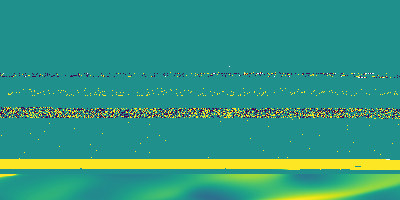
\includegraphics[interpolate=false,width=1.000000in,height=1.000000in]{burgers_rollout_spo_pred_0.01-img0.png}}%
\end{pgfscope}%
\begin{pgfscope}%
\pgfsetbuttcap%
\pgfsetroundjoin%
\definecolor{currentfill}{rgb}{0.000000,0.000000,0.000000}%
\pgfsetfillcolor{currentfill}%
\pgfsetlinewidth{0.803000pt}%
\definecolor{currentstroke}{rgb}{0.000000,0.000000,0.000000}%
\pgfsetstrokecolor{currentstroke}%
\pgfsetdash{}{0pt}%
\pgfsys@defobject{currentmarker}{\pgfqpoint{0.000000in}{-0.048611in}}{\pgfqpoint{0.000000in}{0.000000in}}{%
\pgfpathmoveto{\pgfqpoint{0.000000in}{0.000000in}}%
\pgfpathlineto{\pgfqpoint{0.000000in}{-0.048611in}}%
\pgfusepath{stroke,fill}%
}%
\begin{pgfscope}%
\pgfsys@transformshift{0.726837in}{0.517039in}%
\pgfsys@useobject{currentmarker}{}%
\end{pgfscope}%
\end{pgfscope}%
\begin{pgfscope}%
\definecolor{textcolor}{rgb}{0.000000,0.000000,0.000000}%
\pgfsetstrokecolor{textcolor}%
\pgfsetfillcolor{textcolor}%
\pgftext[x=0.726837in,y=0.419816in,,top]{\color{textcolor}\rmfamily\fontsize{12.000000}{14.400000}\selectfont 0}%
\end{pgfscope}%
\begin{pgfscope}%
\pgfsetbuttcap%
\pgfsetroundjoin%
\definecolor{currentfill}{rgb}{0.000000,0.000000,0.000000}%
\pgfsetfillcolor{currentfill}%
\pgfsetlinewidth{0.803000pt}%
\definecolor{currentstroke}{rgb}{0.000000,0.000000,0.000000}%
\pgfsetstrokecolor{currentstroke}%
\pgfsetdash{}{0pt}%
\pgfsys@defobject{currentmarker}{\pgfqpoint{0.000000in}{-0.048611in}}{\pgfqpoint{0.000000in}{0.000000in}}{%
\pgfpathmoveto{\pgfqpoint{0.000000in}{0.000000in}}%
\pgfpathlineto{\pgfqpoint{0.000000in}{-0.048611in}}%
\pgfusepath{stroke,fill}%
}%
\begin{pgfscope}%
\pgfsys@transformshift{1.495432in}{0.517039in}%
\pgfsys@useobject{currentmarker}{}%
\end{pgfscope}%
\end{pgfscope}%
\begin{pgfscope}%
\definecolor{textcolor}{rgb}{0.000000,0.000000,0.000000}%
\pgfsetstrokecolor{textcolor}%
\pgfsetfillcolor{textcolor}%
\pgftext[x=1.495432in,y=0.419816in,,top]{\color{textcolor}\rmfamily\fontsize{12.000000}{14.400000}\selectfont 1}%
\end{pgfscope}%
\begin{pgfscope}%
\pgfsetbuttcap%
\pgfsetroundjoin%
\definecolor{currentfill}{rgb}{0.000000,0.000000,0.000000}%
\pgfsetfillcolor{currentfill}%
\pgfsetlinewidth{0.803000pt}%
\definecolor{currentstroke}{rgb}{0.000000,0.000000,0.000000}%
\pgfsetstrokecolor{currentstroke}%
\pgfsetdash{}{0pt}%
\pgfsys@defobject{currentmarker}{\pgfqpoint{0.000000in}{-0.048611in}}{\pgfqpoint{0.000000in}{0.000000in}}{%
\pgfpathmoveto{\pgfqpoint{0.000000in}{0.000000in}}%
\pgfpathlineto{\pgfqpoint{0.000000in}{-0.048611in}}%
\pgfusepath{stroke,fill}%
}%
\begin{pgfscope}%
\pgfsys@transformshift{2.264026in}{0.517039in}%
\pgfsys@useobject{currentmarker}{}%
\end{pgfscope}%
\end{pgfscope}%
\begin{pgfscope}%
\definecolor{textcolor}{rgb}{0.000000,0.000000,0.000000}%
\pgfsetstrokecolor{textcolor}%
\pgfsetfillcolor{textcolor}%
\pgftext[x=2.264026in,y=0.419816in,,top]{\color{textcolor}\rmfamily\fontsize{12.000000}{14.400000}\selectfont 2}%
\end{pgfscope}%
\begin{pgfscope}%
\definecolor{textcolor}{rgb}{0.000000,0.000000,0.000000}%
\pgfsetstrokecolor{textcolor}%
\pgfsetfillcolor{textcolor}%
\pgftext[x=1.495432in,y=0.202965in,,top]{\color{textcolor}\rmfamily\fontsize{12.000000}{14.400000}\selectfont Space}%
\end{pgfscope}%
\begin{pgfscope}%
\pgfsetbuttcap%
\pgfsetroundjoin%
\definecolor{currentfill}{rgb}{0.000000,0.000000,0.000000}%
\pgfsetfillcolor{currentfill}%
\pgfsetlinewidth{0.803000pt}%
\definecolor{currentstroke}{rgb}{0.000000,0.000000,0.000000}%
\pgfsetstrokecolor{currentstroke}%
\pgfsetdash{}{0pt}%
\pgfsys@defobject{currentmarker}{\pgfqpoint{-0.048611in}{0.000000in}}{\pgfqpoint{-0.000000in}{0.000000in}}{%
\pgfpathmoveto{\pgfqpoint{-0.000000in}{0.000000in}}%
\pgfpathlineto{\pgfqpoint{-0.048611in}{0.000000in}}%
\pgfusepath{stroke,fill}%
}%
\begin{pgfscope}%
\pgfsys@transformshift{0.726837in}{0.517039in}%
\pgfsys@useobject{currentmarker}{}%
\end{pgfscope}%
\end{pgfscope}%
\begin{pgfscope}%
\definecolor{textcolor}{rgb}{0.000000,0.000000,0.000000}%
\pgfsetstrokecolor{textcolor}%
\pgfsetfillcolor{textcolor}%
\pgftext[x=0.364559in, y=0.453725in, left, base]{\color{textcolor}\rmfamily\fontsize{12.000000}{14.400000}\selectfont 0.0}%
\end{pgfscope}%
\begin{pgfscope}%
\pgfsetbuttcap%
\pgfsetroundjoin%
\definecolor{currentfill}{rgb}{0.000000,0.000000,0.000000}%
\pgfsetfillcolor{currentfill}%
\pgfsetlinewidth{0.803000pt}%
\definecolor{currentstroke}{rgb}{0.000000,0.000000,0.000000}%
\pgfsetstrokecolor{currentstroke}%
\pgfsetdash{}{0pt}%
\pgfsys@defobject{currentmarker}{\pgfqpoint{-0.048611in}{0.000000in}}{\pgfqpoint{-0.000000in}{0.000000in}}{%
\pgfpathmoveto{\pgfqpoint{-0.000000in}{0.000000in}}%
\pgfpathlineto{\pgfqpoint{-0.048611in}{0.000000in}}%
\pgfusepath{stroke,fill}%
}%
\begin{pgfscope}%
\pgfsys@transformshift{0.726837in}{0.861533in}%
\pgfsys@useobject{currentmarker}{}%
\end{pgfscope}%
\end{pgfscope}%
\begin{pgfscope}%
\definecolor{textcolor}{rgb}{0.000000,0.000000,0.000000}%
\pgfsetstrokecolor{textcolor}%
\pgfsetfillcolor{textcolor}%
\pgftext[x=0.364559in, y=0.798219in, left, base]{\color{textcolor}\rmfamily\fontsize{12.000000}{14.400000}\selectfont 2.5}%
\end{pgfscope}%
\begin{pgfscope}%
\pgfsetbuttcap%
\pgfsetroundjoin%
\definecolor{currentfill}{rgb}{0.000000,0.000000,0.000000}%
\pgfsetfillcolor{currentfill}%
\pgfsetlinewidth{0.803000pt}%
\definecolor{currentstroke}{rgb}{0.000000,0.000000,0.000000}%
\pgfsetstrokecolor{currentstroke}%
\pgfsetdash{}{0pt}%
\pgfsys@defobject{currentmarker}{\pgfqpoint{-0.048611in}{0.000000in}}{\pgfqpoint{-0.000000in}{0.000000in}}{%
\pgfpathmoveto{\pgfqpoint{-0.000000in}{0.000000in}}%
\pgfpathlineto{\pgfqpoint{-0.048611in}{0.000000in}}%
\pgfusepath{stroke,fill}%
}%
\begin{pgfscope}%
\pgfsys@transformshift{0.726837in}{1.206027in}%
\pgfsys@useobject{currentmarker}{}%
\end{pgfscope}%
\end{pgfscope}%
\begin{pgfscope}%
\definecolor{textcolor}{rgb}{0.000000,0.000000,0.000000}%
\pgfsetstrokecolor{textcolor}%
\pgfsetfillcolor{textcolor}%
\pgftext[x=0.364559in, y=1.142714in, left, base]{\color{textcolor}\rmfamily\fontsize{12.000000}{14.400000}\selectfont 5.0}%
\end{pgfscope}%
\begin{pgfscope}%
\pgfsetbuttcap%
\pgfsetroundjoin%
\definecolor{currentfill}{rgb}{0.000000,0.000000,0.000000}%
\pgfsetfillcolor{currentfill}%
\pgfsetlinewidth{0.803000pt}%
\definecolor{currentstroke}{rgb}{0.000000,0.000000,0.000000}%
\pgfsetstrokecolor{currentstroke}%
\pgfsetdash{}{0pt}%
\pgfsys@defobject{currentmarker}{\pgfqpoint{-0.048611in}{0.000000in}}{\pgfqpoint{-0.000000in}{0.000000in}}{%
\pgfpathmoveto{\pgfqpoint{-0.000000in}{0.000000in}}%
\pgfpathlineto{\pgfqpoint{-0.048611in}{0.000000in}}%
\pgfusepath{stroke,fill}%
}%
\begin{pgfscope}%
\pgfsys@transformshift{0.726837in}{1.550522in}%
\pgfsys@useobject{currentmarker}{}%
\end{pgfscope}%
\end{pgfscope}%
\begin{pgfscope}%
\definecolor{textcolor}{rgb}{0.000000,0.000000,0.000000}%
\pgfsetstrokecolor{textcolor}%
\pgfsetfillcolor{textcolor}%
\pgftext[x=0.364559in, y=1.487208in, left, base]{\color{textcolor}\rmfamily\fontsize{12.000000}{14.400000}\selectfont 7.5}%
\end{pgfscope}%
\begin{pgfscope}%
\pgfsetbuttcap%
\pgfsetroundjoin%
\definecolor{currentfill}{rgb}{0.000000,0.000000,0.000000}%
\pgfsetfillcolor{currentfill}%
\pgfsetlinewidth{0.803000pt}%
\definecolor{currentstroke}{rgb}{0.000000,0.000000,0.000000}%
\pgfsetstrokecolor{currentstroke}%
\pgfsetdash{}{0pt}%
\pgfsys@defobject{currentmarker}{\pgfqpoint{-0.048611in}{0.000000in}}{\pgfqpoint{-0.000000in}{0.000000in}}{%
\pgfpathmoveto{\pgfqpoint{-0.000000in}{0.000000in}}%
\pgfpathlineto{\pgfqpoint{-0.048611in}{0.000000in}}%
\pgfusepath{stroke,fill}%
}%
\begin{pgfscope}%
\pgfsys@transformshift{0.726837in}{1.895016in}%
\pgfsys@useobject{currentmarker}{}%
\end{pgfscope}%
\end{pgfscope}%
\begin{pgfscope}%
\definecolor{textcolor}{rgb}{0.000000,0.000000,0.000000}%
\pgfsetstrokecolor{textcolor}%
\pgfsetfillcolor{textcolor}%
\pgftext[x=0.258521in, y=1.831702in, left, base]{\color{textcolor}\rmfamily\fontsize{12.000000}{14.400000}\selectfont 10.0}%
\end{pgfscope}%
\begin{pgfscope}%
\definecolor{textcolor}{rgb}{0.000000,0.000000,0.000000}%
\pgfsetstrokecolor{textcolor}%
\pgfsetfillcolor{textcolor}%
\pgftext[x=0.202965in,y=1.206027in,,bottom,rotate=90.000000]{\color{textcolor}\rmfamily\fontsize{12.000000}{14.400000}\selectfont Time}%
\end{pgfscope}%
\begin{pgfscope}%
\pgfsetrectcap%
\pgfsetmiterjoin%
\pgfsetlinewidth{0.803000pt}%
\definecolor{currentstroke}{rgb}{0.000000,0.000000,0.000000}%
\pgfsetstrokecolor{currentstroke}%
\pgfsetdash{}{0pt}%
\pgfpathmoveto{\pgfqpoint{0.726837in}{0.517039in}}%
\pgfpathlineto{\pgfqpoint{0.726837in}{1.895016in}}%
\pgfusepath{stroke}%
\end{pgfscope}%
\begin{pgfscope}%
\pgfsetrectcap%
\pgfsetmiterjoin%
\pgfsetlinewidth{0.803000pt}%
\definecolor{currentstroke}{rgb}{0.000000,0.000000,0.000000}%
\pgfsetstrokecolor{currentstroke}%
\pgfsetdash{}{0pt}%
\pgfpathmoveto{\pgfqpoint{2.264026in}{0.517039in}}%
\pgfpathlineto{\pgfqpoint{2.264026in}{1.895016in}}%
\pgfusepath{stroke}%
\end{pgfscope}%
\begin{pgfscope}%
\pgfsetrectcap%
\pgfsetmiterjoin%
\pgfsetlinewidth{0.803000pt}%
\definecolor{currentstroke}{rgb}{0.000000,0.000000,0.000000}%
\pgfsetstrokecolor{currentstroke}%
\pgfsetdash{}{0pt}%
\pgfpathmoveto{\pgfqpoint{0.726837in}{0.517039in}}%
\pgfpathlineto{\pgfqpoint{2.264026in}{0.517039in}}%
\pgfusepath{stroke}%
\end{pgfscope}%
\begin{pgfscope}%
\pgfsetrectcap%
\pgfsetmiterjoin%
\pgfsetlinewidth{0.803000pt}%
\definecolor{currentstroke}{rgb}{0.000000,0.000000,0.000000}%
\pgfsetstrokecolor{currentstroke}%
\pgfsetdash{}{0pt}%
\pgfpathmoveto{\pgfqpoint{0.726837in}{1.895016in}}%
\pgfpathlineto{\pgfqpoint{2.264026in}{1.895016in}}%
\pgfusepath{stroke}%
\end{pgfscope}%
\begin{pgfscope}%
\pgfsetbuttcap%
\pgfsetmiterjoin%
\pgfsetlinewidth{0.000000pt}%
\definecolor{currentstroke}{rgb}{0.000000,0.000000,0.000000}%
\pgfsetstrokecolor{currentstroke}%
\pgfsetstrokeopacity{0.000000}%
\pgfsetdash{}{0pt}%
\pgfpathmoveto{\pgfqpoint{2.393905in}{0.517039in}}%
\pgfpathlineto{\pgfqpoint{2.462804in}{0.517039in}}%
\pgfpathlineto{\pgfqpoint{2.462804in}{1.895016in}}%
\pgfpathlineto{\pgfqpoint{2.393905in}{1.895016in}}%
\pgfpathlineto{\pgfqpoint{2.393905in}{0.517039in}}%
\pgfpathclose%
\pgfusepath{}%
\end{pgfscope}%
\begin{pgfscope}%
\pgfsys@transformshift{2.390000in}{0.520000in}%
\pgftext[left,bottom]{
\includegraphics[interpolate=true,width=0.070000in,height=1.380000in]{burgers_rollout_spo_pred_0.01-img1.png}}%
\end{pgfscope}%
\begin{pgfscope}%
\pgfsetbuttcap%
\pgfsetroundjoin%
\definecolor{currentfill}{rgb}{0.000000,0.000000,0.000000}%
\pgfsetfillcolor{currentfill}%
\pgfsetlinewidth{0.803000pt}%
\definecolor{currentstroke}{rgb}{0.000000,0.000000,0.000000}%
\pgfsetstrokecolor{currentstroke}%
\pgfsetdash{}{0pt}%
\pgfsys@defobject{currentmarker}{\pgfqpoint{0.000000in}{0.000000in}}{\pgfqpoint{0.048611in}{0.000000in}}{%
\pgfpathmoveto{\pgfqpoint{0.000000in}{0.000000in}}%
\pgfpathlineto{\pgfqpoint{0.048611in}{0.000000in}}%
\pgfusepath{stroke,fill}%
}%
\begin{pgfscope}%
\pgfsys@transformshift{2.462804in}{0.839076in}%
\pgfsys@useobject{currentmarker}{}%
\end{pgfscope}%
\end{pgfscope}%
\begin{pgfscope}%
\definecolor{textcolor}{rgb}{0.000000,0.000000,0.000000}%
\pgfsetstrokecolor{textcolor}%
\pgfsetfillcolor{textcolor}%
\pgftext[x=2.560026in, y=0.775762in, left, base]{\color{textcolor}\rmfamily\fontsize{12.000000}{14.400000}\selectfont \ensuremath{-}0.5}%
\end{pgfscope}%
\begin{pgfscope}%
\pgfsetbuttcap%
\pgfsetroundjoin%
\definecolor{currentfill}{rgb}{0.000000,0.000000,0.000000}%
\pgfsetfillcolor{currentfill}%
\pgfsetlinewidth{0.803000pt}%
\definecolor{currentstroke}{rgb}{0.000000,0.000000,0.000000}%
\pgfsetstrokecolor{currentstroke}%
\pgfsetdash{}{0pt}%
\pgfsys@defobject{currentmarker}{\pgfqpoint{0.000000in}{0.000000in}}{\pgfqpoint{0.048611in}{0.000000in}}{%
\pgfpathmoveto{\pgfqpoint{0.000000in}{0.000000in}}%
\pgfpathlineto{\pgfqpoint{0.048611in}{0.000000in}}%
\pgfusepath{stroke,fill}%
}%
\begin{pgfscope}%
\pgfsys@transformshift{2.462804in}{1.206027in}%
\pgfsys@useobject{currentmarker}{}%
\end{pgfscope}%
\end{pgfscope}%
\begin{pgfscope}%
\definecolor{textcolor}{rgb}{0.000000,0.000000,0.000000}%
\pgfsetstrokecolor{textcolor}%
\pgfsetfillcolor{textcolor}%
\pgftext[x=2.560026in, y=1.142714in, left, base]{\color{textcolor}\rmfamily\fontsize{12.000000}{14.400000}\selectfont 0.0}%
\end{pgfscope}%
\begin{pgfscope}%
\pgfsetbuttcap%
\pgfsetroundjoin%
\definecolor{currentfill}{rgb}{0.000000,0.000000,0.000000}%
\pgfsetfillcolor{currentfill}%
\pgfsetlinewidth{0.803000pt}%
\definecolor{currentstroke}{rgb}{0.000000,0.000000,0.000000}%
\pgfsetstrokecolor{currentstroke}%
\pgfsetdash{}{0pt}%
\pgfsys@defobject{currentmarker}{\pgfqpoint{0.000000in}{0.000000in}}{\pgfqpoint{0.048611in}{0.000000in}}{%
\pgfpathmoveto{\pgfqpoint{0.000000in}{0.000000in}}%
\pgfpathlineto{\pgfqpoint{0.048611in}{0.000000in}}%
\pgfusepath{stroke,fill}%
}%
\begin{pgfscope}%
\pgfsys@transformshift{2.462804in}{1.572979in}%
\pgfsys@useobject{currentmarker}{}%
\end{pgfscope}%
\end{pgfscope}%
\begin{pgfscope}%
\definecolor{textcolor}{rgb}{0.000000,0.000000,0.000000}%
\pgfsetstrokecolor{textcolor}%
\pgfsetfillcolor{textcolor}%
\pgftext[x=2.560026in, y=1.509665in, left, base]{\color{textcolor}\rmfamily\fontsize{12.000000}{14.400000}\selectfont 0.5}%
\end{pgfscope}%
\begin{pgfscope}%
\pgfsetrectcap%
\pgfsetmiterjoin%
\pgfsetlinewidth{0.803000pt}%
\definecolor{currentstroke}{rgb}{0.000000,0.000000,0.000000}%
\pgfsetstrokecolor{currentstroke}%
\pgfsetdash{}{0pt}%
\pgfpathmoveto{\pgfqpoint{2.393905in}{0.517039in}}%
\pgfpathlineto{\pgfqpoint{2.428354in}{0.517039in}}%
\pgfpathlineto{\pgfqpoint{2.462804in}{0.517039in}}%
\pgfpathlineto{\pgfqpoint{2.462804in}{1.895016in}}%
\pgfpathlineto{\pgfqpoint{2.428354in}{1.895016in}}%
\pgfpathlineto{\pgfqpoint{2.393905in}{1.895016in}}%
\pgfpathlineto{\pgfqpoint{2.393905in}{0.517039in}}%
\pgfpathclose%
\pgfusepath{stroke}%
\end{pgfscope}%
\end{pgfpicture}%
\makeatother%
\endgroup%

      \end{adjustbox}
      \caption{lsoda prediction.}\label{fig:comp_spo_pred_0.01}
    \end{subfigure}
    \begin{subfigure}{0.49\linewidth}
      \begin{adjustbox}{width=\linewidth}
        \begingroup%
\makeatletter%
\begin{pgfpicture}%
\pgfpathrectangle{\pgfpointorigin}{\pgfqpoint{3.000000in}{2.000000in}}%
\pgfusepath{use as bounding box, clip}%
\begin{pgfscope}%
\pgfsetbuttcap%
\pgfsetmiterjoin%
\pgfsetlinewidth{0.000000pt}%
\definecolor{currentstroke}{rgb}{0.000000,0.000000,0.000000}%
\pgfsetstrokecolor{currentstroke}%
\pgfsetstrokeopacity{0.000000}%
\pgfsetdash{}{0pt}%
\pgfpathmoveto{\pgfqpoint{0.000000in}{0.000000in}}%
\pgfpathlineto{\pgfqpoint{3.000000in}{0.000000in}}%
\pgfpathlineto{\pgfqpoint{3.000000in}{2.000000in}}%
\pgfpathlineto{\pgfqpoint{0.000000in}{2.000000in}}%
\pgfpathlineto{\pgfqpoint{0.000000in}{0.000000in}}%
\pgfpathclose%
\pgfusepath{}%
\end{pgfscope}%
\begin{pgfscope}%
\pgfsetbuttcap%
\pgfsetmiterjoin%
\pgfsetlinewidth{0.000000pt}%
\definecolor{currentstroke}{rgb}{0.000000,0.000000,0.000000}%
\pgfsetstrokecolor{currentstroke}%
\pgfsetstrokeopacity{0.000000}%
\pgfsetdash{}{0pt}%
\pgfpathmoveto{\pgfqpoint{0.726837in}{0.517039in}}%
\pgfpathlineto{\pgfqpoint{2.264026in}{0.517039in}}%
\pgfpathlineto{\pgfqpoint{2.264026in}{1.895016in}}%
\pgfpathlineto{\pgfqpoint{0.726837in}{1.895016in}}%
\pgfpathlineto{\pgfqpoint{0.726837in}{0.517039in}}%
\pgfpathclose%
\pgfusepath{}%
\end{pgfscope}%
\begin{pgfscope}%
\pgfpathrectangle{\pgfqpoint{0.726837in}{0.517039in}}{\pgfqpoint{1.537189in}{1.377978in}}%
\pgfusepath{clip}%
\pgfsys@transformcm{1.537189}{0.000000}{0.000000}{1.377978}{0.726837in}{0.517039in}%
\pgftext[left,bottom]{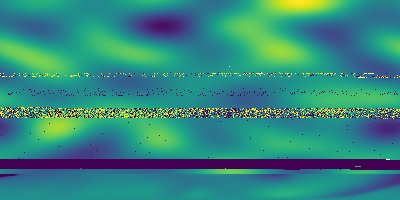
\includegraphics[interpolate=false,width=1.000000in,height=1.000000in]{burgers_rollout_spo_diff_0.01-img0.png}}%
\end{pgfscope}%
\begin{pgfscope}%
\pgfsetbuttcap%
\pgfsetroundjoin%
\definecolor{currentfill}{rgb}{0.000000,0.000000,0.000000}%
\pgfsetfillcolor{currentfill}%
\pgfsetlinewidth{0.803000pt}%
\definecolor{currentstroke}{rgb}{0.000000,0.000000,0.000000}%
\pgfsetstrokecolor{currentstroke}%
\pgfsetdash{}{0pt}%
\pgfsys@defobject{currentmarker}{\pgfqpoint{0.000000in}{-0.048611in}}{\pgfqpoint{0.000000in}{0.000000in}}{%
\pgfpathmoveto{\pgfqpoint{0.000000in}{0.000000in}}%
\pgfpathlineto{\pgfqpoint{0.000000in}{-0.048611in}}%
\pgfusepath{stroke,fill}%
}%
\begin{pgfscope}%
\pgfsys@transformshift{0.726837in}{0.517039in}%
\pgfsys@useobject{currentmarker}{}%
\end{pgfscope}%
\end{pgfscope}%
\begin{pgfscope}%
\definecolor{textcolor}{rgb}{0.000000,0.000000,0.000000}%
\pgfsetstrokecolor{textcolor}%
\pgfsetfillcolor{textcolor}%
\pgftext[x=0.726837in,y=0.419816in,,top]{\color{textcolor}\rmfamily\fontsize{12.000000}{14.400000}\selectfont 0}%
\end{pgfscope}%
\begin{pgfscope}%
\pgfsetbuttcap%
\pgfsetroundjoin%
\definecolor{currentfill}{rgb}{0.000000,0.000000,0.000000}%
\pgfsetfillcolor{currentfill}%
\pgfsetlinewidth{0.803000pt}%
\definecolor{currentstroke}{rgb}{0.000000,0.000000,0.000000}%
\pgfsetstrokecolor{currentstroke}%
\pgfsetdash{}{0pt}%
\pgfsys@defobject{currentmarker}{\pgfqpoint{0.000000in}{-0.048611in}}{\pgfqpoint{0.000000in}{0.000000in}}{%
\pgfpathmoveto{\pgfqpoint{0.000000in}{0.000000in}}%
\pgfpathlineto{\pgfqpoint{0.000000in}{-0.048611in}}%
\pgfusepath{stroke,fill}%
}%
\begin{pgfscope}%
\pgfsys@transformshift{1.495432in}{0.517039in}%
\pgfsys@useobject{currentmarker}{}%
\end{pgfscope}%
\end{pgfscope}%
\begin{pgfscope}%
\definecolor{textcolor}{rgb}{0.000000,0.000000,0.000000}%
\pgfsetstrokecolor{textcolor}%
\pgfsetfillcolor{textcolor}%
\pgftext[x=1.495432in,y=0.419816in,,top]{\color{textcolor}\rmfamily\fontsize{12.000000}{14.400000}\selectfont 1}%
\end{pgfscope}%
\begin{pgfscope}%
\pgfsetbuttcap%
\pgfsetroundjoin%
\definecolor{currentfill}{rgb}{0.000000,0.000000,0.000000}%
\pgfsetfillcolor{currentfill}%
\pgfsetlinewidth{0.803000pt}%
\definecolor{currentstroke}{rgb}{0.000000,0.000000,0.000000}%
\pgfsetstrokecolor{currentstroke}%
\pgfsetdash{}{0pt}%
\pgfsys@defobject{currentmarker}{\pgfqpoint{0.000000in}{-0.048611in}}{\pgfqpoint{0.000000in}{0.000000in}}{%
\pgfpathmoveto{\pgfqpoint{0.000000in}{0.000000in}}%
\pgfpathlineto{\pgfqpoint{0.000000in}{-0.048611in}}%
\pgfusepath{stroke,fill}%
}%
\begin{pgfscope}%
\pgfsys@transformshift{2.264026in}{0.517039in}%
\pgfsys@useobject{currentmarker}{}%
\end{pgfscope}%
\end{pgfscope}%
\begin{pgfscope}%
\definecolor{textcolor}{rgb}{0.000000,0.000000,0.000000}%
\pgfsetstrokecolor{textcolor}%
\pgfsetfillcolor{textcolor}%
\pgftext[x=2.264026in,y=0.419816in,,top]{\color{textcolor}\rmfamily\fontsize{12.000000}{14.400000}\selectfont 2}%
\end{pgfscope}%
\begin{pgfscope}%
\definecolor{textcolor}{rgb}{0.000000,0.000000,0.000000}%
\pgfsetstrokecolor{textcolor}%
\pgfsetfillcolor{textcolor}%
\pgftext[x=1.495432in,y=0.202965in,,top]{\color{textcolor}\rmfamily\fontsize{12.000000}{14.400000}\selectfont Space}%
\end{pgfscope}%
\begin{pgfscope}%
\pgfsetbuttcap%
\pgfsetroundjoin%
\definecolor{currentfill}{rgb}{0.000000,0.000000,0.000000}%
\pgfsetfillcolor{currentfill}%
\pgfsetlinewidth{0.803000pt}%
\definecolor{currentstroke}{rgb}{0.000000,0.000000,0.000000}%
\pgfsetstrokecolor{currentstroke}%
\pgfsetdash{}{0pt}%
\pgfsys@defobject{currentmarker}{\pgfqpoint{-0.048611in}{0.000000in}}{\pgfqpoint{-0.000000in}{0.000000in}}{%
\pgfpathmoveto{\pgfqpoint{-0.000000in}{0.000000in}}%
\pgfpathlineto{\pgfqpoint{-0.048611in}{0.000000in}}%
\pgfusepath{stroke,fill}%
}%
\begin{pgfscope}%
\pgfsys@transformshift{0.726837in}{0.517039in}%
\pgfsys@useobject{currentmarker}{}%
\end{pgfscope}%
\end{pgfscope}%
\begin{pgfscope}%
\definecolor{textcolor}{rgb}{0.000000,0.000000,0.000000}%
\pgfsetstrokecolor{textcolor}%
\pgfsetfillcolor{textcolor}%
\pgftext[x=0.364559in, y=0.453725in, left, base]{\color{textcolor}\rmfamily\fontsize{12.000000}{14.400000}\selectfont 0.0}%
\end{pgfscope}%
\begin{pgfscope}%
\pgfsetbuttcap%
\pgfsetroundjoin%
\definecolor{currentfill}{rgb}{0.000000,0.000000,0.000000}%
\pgfsetfillcolor{currentfill}%
\pgfsetlinewidth{0.803000pt}%
\definecolor{currentstroke}{rgb}{0.000000,0.000000,0.000000}%
\pgfsetstrokecolor{currentstroke}%
\pgfsetdash{}{0pt}%
\pgfsys@defobject{currentmarker}{\pgfqpoint{-0.048611in}{0.000000in}}{\pgfqpoint{-0.000000in}{0.000000in}}{%
\pgfpathmoveto{\pgfqpoint{-0.000000in}{0.000000in}}%
\pgfpathlineto{\pgfqpoint{-0.048611in}{0.000000in}}%
\pgfusepath{stroke,fill}%
}%
\begin{pgfscope}%
\pgfsys@transformshift{0.726837in}{0.861533in}%
\pgfsys@useobject{currentmarker}{}%
\end{pgfscope}%
\end{pgfscope}%
\begin{pgfscope}%
\definecolor{textcolor}{rgb}{0.000000,0.000000,0.000000}%
\pgfsetstrokecolor{textcolor}%
\pgfsetfillcolor{textcolor}%
\pgftext[x=0.364559in, y=0.798219in, left, base]{\color{textcolor}\rmfamily\fontsize{12.000000}{14.400000}\selectfont 2.5}%
\end{pgfscope}%
\begin{pgfscope}%
\pgfsetbuttcap%
\pgfsetroundjoin%
\definecolor{currentfill}{rgb}{0.000000,0.000000,0.000000}%
\pgfsetfillcolor{currentfill}%
\pgfsetlinewidth{0.803000pt}%
\definecolor{currentstroke}{rgb}{0.000000,0.000000,0.000000}%
\pgfsetstrokecolor{currentstroke}%
\pgfsetdash{}{0pt}%
\pgfsys@defobject{currentmarker}{\pgfqpoint{-0.048611in}{0.000000in}}{\pgfqpoint{-0.000000in}{0.000000in}}{%
\pgfpathmoveto{\pgfqpoint{-0.000000in}{0.000000in}}%
\pgfpathlineto{\pgfqpoint{-0.048611in}{0.000000in}}%
\pgfusepath{stroke,fill}%
}%
\begin{pgfscope}%
\pgfsys@transformshift{0.726837in}{1.206027in}%
\pgfsys@useobject{currentmarker}{}%
\end{pgfscope}%
\end{pgfscope}%
\begin{pgfscope}%
\definecolor{textcolor}{rgb}{0.000000,0.000000,0.000000}%
\pgfsetstrokecolor{textcolor}%
\pgfsetfillcolor{textcolor}%
\pgftext[x=0.364559in, y=1.142714in, left, base]{\color{textcolor}\rmfamily\fontsize{12.000000}{14.400000}\selectfont 5.0}%
\end{pgfscope}%
\begin{pgfscope}%
\pgfsetbuttcap%
\pgfsetroundjoin%
\definecolor{currentfill}{rgb}{0.000000,0.000000,0.000000}%
\pgfsetfillcolor{currentfill}%
\pgfsetlinewidth{0.803000pt}%
\definecolor{currentstroke}{rgb}{0.000000,0.000000,0.000000}%
\pgfsetstrokecolor{currentstroke}%
\pgfsetdash{}{0pt}%
\pgfsys@defobject{currentmarker}{\pgfqpoint{-0.048611in}{0.000000in}}{\pgfqpoint{-0.000000in}{0.000000in}}{%
\pgfpathmoveto{\pgfqpoint{-0.000000in}{0.000000in}}%
\pgfpathlineto{\pgfqpoint{-0.048611in}{0.000000in}}%
\pgfusepath{stroke,fill}%
}%
\begin{pgfscope}%
\pgfsys@transformshift{0.726837in}{1.550522in}%
\pgfsys@useobject{currentmarker}{}%
\end{pgfscope}%
\end{pgfscope}%
\begin{pgfscope}%
\definecolor{textcolor}{rgb}{0.000000,0.000000,0.000000}%
\pgfsetstrokecolor{textcolor}%
\pgfsetfillcolor{textcolor}%
\pgftext[x=0.364559in, y=1.487208in, left, base]{\color{textcolor}\rmfamily\fontsize{12.000000}{14.400000}\selectfont 7.5}%
\end{pgfscope}%
\begin{pgfscope}%
\pgfsetbuttcap%
\pgfsetroundjoin%
\definecolor{currentfill}{rgb}{0.000000,0.000000,0.000000}%
\pgfsetfillcolor{currentfill}%
\pgfsetlinewidth{0.803000pt}%
\definecolor{currentstroke}{rgb}{0.000000,0.000000,0.000000}%
\pgfsetstrokecolor{currentstroke}%
\pgfsetdash{}{0pt}%
\pgfsys@defobject{currentmarker}{\pgfqpoint{-0.048611in}{0.000000in}}{\pgfqpoint{-0.000000in}{0.000000in}}{%
\pgfpathmoveto{\pgfqpoint{-0.000000in}{0.000000in}}%
\pgfpathlineto{\pgfqpoint{-0.048611in}{0.000000in}}%
\pgfusepath{stroke,fill}%
}%
\begin{pgfscope}%
\pgfsys@transformshift{0.726837in}{1.895016in}%
\pgfsys@useobject{currentmarker}{}%
\end{pgfscope}%
\end{pgfscope}%
\begin{pgfscope}%
\definecolor{textcolor}{rgb}{0.000000,0.000000,0.000000}%
\pgfsetstrokecolor{textcolor}%
\pgfsetfillcolor{textcolor}%
\pgftext[x=0.258521in, y=1.831702in, left, base]{\color{textcolor}\rmfamily\fontsize{12.000000}{14.400000}\selectfont 10.0}%
\end{pgfscope}%
\begin{pgfscope}%
\definecolor{textcolor}{rgb}{0.000000,0.000000,0.000000}%
\pgfsetstrokecolor{textcolor}%
\pgfsetfillcolor{textcolor}%
\pgftext[x=0.202965in,y=1.206027in,,bottom,rotate=90.000000]{\color{textcolor}\rmfamily\fontsize{12.000000}{14.400000}\selectfont Time}%
\end{pgfscope}%
\begin{pgfscope}%
\pgfsetrectcap%
\pgfsetmiterjoin%
\pgfsetlinewidth{0.803000pt}%
\definecolor{currentstroke}{rgb}{0.000000,0.000000,0.000000}%
\pgfsetstrokecolor{currentstroke}%
\pgfsetdash{}{0pt}%
\pgfpathmoveto{\pgfqpoint{0.726837in}{0.517039in}}%
\pgfpathlineto{\pgfqpoint{0.726837in}{1.895016in}}%
\pgfusepath{stroke}%
\end{pgfscope}%
\begin{pgfscope}%
\pgfsetrectcap%
\pgfsetmiterjoin%
\pgfsetlinewidth{0.803000pt}%
\definecolor{currentstroke}{rgb}{0.000000,0.000000,0.000000}%
\pgfsetstrokecolor{currentstroke}%
\pgfsetdash{}{0pt}%
\pgfpathmoveto{\pgfqpoint{2.264026in}{0.517039in}}%
\pgfpathlineto{\pgfqpoint{2.264026in}{1.895016in}}%
\pgfusepath{stroke}%
\end{pgfscope}%
\begin{pgfscope}%
\pgfsetrectcap%
\pgfsetmiterjoin%
\pgfsetlinewidth{0.803000pt}%
\definecolor{currentstroke}{rgb}{0.000000,0.000000,0.000000}%
\pgfsetstrokecolor{currentstroke}%
\pgfsetdash{}{0pt}%
\pgfpathmoveto{\pgfqpoint{0.726837in}{0.517039in}}%
\pgfpathlineto{\pgfqpoint{2.264026in}{0.517039in}}%
\pgfusepath{stroke}%
\end{pgfscope}%
\begin{pgfscope}%
\pgfsetrectcap%
\pgfsetmiterjoin%
\pgfsetlinewidth{0.803000pt}%
\definecolor{currentstroke}{rgb}{0.000000,0.000000,0.000000}%
\pgfsetstrokecolor{currentstroke}%
\pgfsetdash{}{0pt}%
\pgfpathmoveto{\pgfqpoint{0.726837in}{1.895016in}}%
\pgfpathlineto{\pgfqpoint{2.264026in}{1.895016in}}%
\pgfusepath{stroke}%
\end{pgfscope}%
\begin{pgfscope}%
\pgfsetbuttcap%
\pgfsetmiterjoin%
\pgfsetlinewidth{0.000000pt}%
\definecolor{currentstroke}{rgb}{0.000000,0.000000,0.000000}%
\pgfsetstrokecolor{currentstroke}%
\pgfsetstrokeopacity{0.000000}%
\pgfsetdash{}{0pt}%
\pgfpathmoveto{\pgfqpoint{2.393905in}{0.517039in}}%
\pgfpathlineto{\pgfqpoint{2.462804in}{0.517039in}}%
\pgfpathlineto{\pgfqpoint{2.462804in}{1.895016in}}%
\pgfpathlineto{\pgfqpoint{2.393905in}{1.895016in}}%
\pgfpathlineto{\pgfqpoint{2.393905in}{0.517039in}}%
\pgfpathclose%
\pgfusepath{}%
\end{pgfscope}%
\begin{pgfscope}%
\pgfsys@transformshift{2.390000in}{0.520000in}%
\pgftext[left,bottom]{
\includegraphics[interpolate=true,width=0.070000in,height=1.380000in]{burgers_rollout_spo_diff_0.01-img1.png}}%
\end{pgfscope}%
\begin{pgfscope}%
\pgfsetbuttcap%
\pgfsetroundjoin%
\definecolor{currentfill}{rgb}{0.000000,0.000000,0.000000}%
\pgfsetfillcolor{currentfill}%
\pgfsetlinewidth{0.803000pt}%
\definecolor{currentstroke}{rgb}{0.000000,0.000000,0.000000}%
\pgfsetstrokecolor{currentstroke}%
\pgfsetdash{}{0pt}%
\pgfsys@defobject{currentmarker}{\pgfqpoint{0.000000in}{0.000000in}}{\pgfqpoint{0.048611in}{0.000000in}}{%
\pgfpathmoveto{\pgfqpoint{0.000000in}{0.000000in}}%
\pgfpathlineto{\pgfqpoint{0.048611in}{0.000000in}}%
\pgfusepath{stroke,fill}%
}%
\begin{pgfscope}%
\pgfsys@transformshift{2.462804in}{0.839076in}%
\pgfsys@useobject{currentmarker}{}%
\end{pgfscope}%
\end{pgfscope}%
\begin{pgfscope}%
\definecolor{textcolor}{rgb}{0.000000,0.000000,0.000000}%
\pgfsetstrokecolor{textcolor}%
\pgfsetfillcolor{textcolor}%
\pgftext[x=2.560026in, y=0.775762in, left, base]{\color{textcolor}\rmfamily\fontsize{12.000000}{14.400000}\selectfont \ensuremath{-}0.5}%
\end{pgfscope}%
\begin{pgfscope}%
\pgfsetbuttcap%
\pgfsetroundjoin%
\definecolor{currentfill}{rgb}{0.000000,0.000000,0.000000}%
\pgfsetfillcolor{currentfill}%
\pgfsetlinewidth{0.803000pt}%
\definecolor{currentstroke}{rgb}{0.000000,0.000000,0.000000}%
\pgfsetstrokecolor{currentstroke}%
\pgfsetdash{}{0pt}%
\pgfsys@defobject{currentmarker}{\pgfqpoint{0.000000in}{0.000000in}}{\pgfqpoint{0.048611in}{0.000000in}}{%
\pgfpathmoveto{\pgfqpoint{0.000000in}{0.000000in}}%
\pgfpathlineto{\pgfqpoint{0.048611in}{0.000000in}}%
\pgfusepath{stroke,fill}%
}%
\begin{pgfscope}%
\pgfsys@transformshift{2.462804in}{1.206027in}%
\pgfsys@useobject{currentmarker}{}%
\end{pgfscope}%
\end{pgfscope}%
\begin{pgfscope}%
\definecolor{textcolor}{rgb}{0.000000,0.000000,0.000000}%
\pgfsetstrokecolor{textcolor}%
\pgfsetfillcolor{textcolor}%
\pgftext[x=2.560026in, y=1.142714in, left, base]{\color{textcolor}\rmfamily\fontsize{12.000000}{14.400000}\selectfont 0.0}%
\end{pgfscope}%
\begin{pgfscope}%
\pgfsetbuttcap%
\pgfsetroundjoin%
\definecolor{currentfill}{rgb}{0.000000,0.000000,0.000000}%
\pgfsetfillcolor{currentfill}%
\pgfsetlinewidth{0.803000pt}%
\definecolor{currentstroke}{rgb}{0.000000,0.000000,0.000000}%
\pgfsetstrokecolor{currentstroke}%
\pgfsetdash{}{0pt}%
\pgfsys@defobject{currentmarker}{\pgfqpoint{0.000000in}{0.000000in}}{\pgfqpoint{0.048611in}{0.000000in}}{%
\pgfpathmoveto{\pgfqpoint{0.000000in}{0.000000in}}%
\pgfpathlineto{\pgfqpoint{0.048611in}{0.000000in}}%
\pgfusepath{stroke,fill}%
}%
\begin{pgfscope}%
\pgfsys@transformshift{2.462804in}{1.572979in}%
\pgfsys@useobject{currentmarker}{}%
\end{pgfscope}%
\end{pgfscope}%
\begin{pgfscope}%
\definecolor{textcolor}{rgb}{0.000000,0.000000,0.000000}%
\pgfsetstrokecolor{textcolor}%
\pgfsetfillcolor{textcolor}%
\pgftext[x=2.560026in, y=1.509665in, left, base]{\color{textcolor}\rmfamily\fontsize{12.000000}{14.400000}\selectfont 0.5}%
\end{pgfscope}%
\begin{pgfscope}%
\pgfsetrectcap%
\pgfsetmiterjoin%
\pgfsetlinewidth{0.803000pt}%
\definecolor{currentstroke}{rgb}{0.000000,0.000000,0.000000}%
\pgfsetstrokecolor{currentstroke}%
\pgfsetdash{}{0pt}%
\pgfpathmoveto{\pgfqpoint{2.393905in}{0.517039in}}%
\pgfpathlineto{\pgfqpoint{2.428354in}{0.517039in}}%
\pgfpathlineto{\pgfqpoint{2.462804in}{0.517039in}}%
\pgfpathlineto{\pgfqpoint{2.462804in}{1.895016in}}%
\pgfpathlineto{\pgfqpoint{2.428354in}{1.895016in}}%
\pgfpathlineto{\pgfqpoint{2.393905in}{1.895016in}}%
\pgfpathlineto{\pgfqpoint{2.393905in}{0.517039in}}%
\pgfpathclose%
\pgfusepath{stroke}%
\end{pgfscope}%
\end{pgfpicture}%
\makeatother%
\endgroup%

      \end{adjustbox}
      \caption{lsoda difference with target.}\label{fig:comp_spo_diff_0.01}
    \end{subfigure}
  \end{adjustwidth}
  \caption{Comparison of our model (SpectralSVR) and numerical methods for the Forced Burgers equation with viscosity \(\nu=0.01\).}\label{fig:comparison_burgers_0.01}
\end{figure}
\begin{table}[H]
  \caption{Metrics for predicting the exact solution for SpectralSVR (Ours) method.}\label{table:comparison_exact_metrics_lssvr}
  \centering
  \begin{tabular}{lcccc}
    \toprule
    \(\nu \) & MSE  & RMSE & MAE  & sMAPE \\
    \midrule
    0.0      & 0.01 & 0.07 & 0.06 & 1.99  \\
    0.01     & 0.00 & 0.07 & 0.06 & 1.61  \\
    0.1      & 0.00 & 0.02 & 0.02 & 1.47  \\
    \bottomrule
  \end{tabular}
\end{table}
\begin{table}[H]
  \caption{Metrics for predicting the exact solution for SpectralSVR (FNN) baseline method.}\label{table:comparison_exact_metrics_fnn}
  \centering
  \begin{tabular}{lcccc}
    \toprule
    \(\nu \) & MSE & RMSE & MAE & sMAPE \\
    \midrule
    0.0      & inf & inf  & inf & 1.99  \\
    0.01     & inf & inf  & inf & 1.98  \\
    0.1      & inf & inf  & inf & 1.98  \\
    \bottomrule
  \end{tabular}
\end{table}
\begin{table}[H]
  \caption{Metrics for predicting the exact solution for the lsoda method.}\label{table:comparison_exact_metrics_lsoda}
  \centering
  \begin{tabular}{lcccc}
    \toprule
    \(\nu \) & MSE  & RMSE & MAE  & sMAPE \\
    \midrule
    0.0      & 0.00 & 0.00 & 0.00 & 0.00  \\
    0.01     & 0.00 & 0.00 & 0.00 & 0.08  \\
    0.1      & 0.00 & 0.04 & 0.04 & 1.52  \\
    \bottomrule
  \end{tabular}
\end{table}
\begin{table}[H]
  \caption{Metrics for predicting the exact solution for the IABM method.}\label{table:comparison_exact_metrics_iabm}
  \centering
  \begin{tabular}{lcccc}
    \toprule
    \(\nu \) & MSE  & RMSE & MAE  & sMAPE \\
    \midrule
    0.0      & 0.00 & 0.00 & 0.00 & 0.00  \\
    0.01     & nan  & nan  & nan  & nan   \\
    0.1      & nan  & nan  & nan  & nan   \\
    \bottomrule
  \end{tabular}
\end{table}